% Definiciones y constantes de estilo
% Clase del documento
\documentclass[a4paper,12pt,oneside,openright,titlepage]{book}

%
% Paquetes necesarios
%

% Símbolo del euro
\usepackage{eurosym}
% Codificación UTF8
\usepackage[utf8]{inputenc}
% Caracteres del español
\usepackage[spanish]{babel}
% Código, algoritmos, etc.
\usepackage{listings}
% Definición de colores
\usepackage{color}
% Extensión del paquete color
\usepackage[table,xcdraw]{xcolor}
% Márgenes
\usepackage{anysize}
% Cabecera y pie de página
\usepackage{fancyhdr}
% Estilo título capítulos
\usepackage{quotchap}
% Algoritmos (expresarlos mejor)
\usepackage{algorithmic}
% Títulos de secciones
\usepackage{titlesec}
% Fórmulas matemáticas
\usepackage[cmex10]{amsmath}
% Enumeraciones
\usepackage{enumerate}
% Páginas en blanco
\usepackage{emptypage}
% Separación entre cajas
\usepackage{float}
% Imágenes
\usepackage[pdftex]{graphicx}
% Mejora de las tablas
\usepackage{array}
% Mejora de los símbolos matemáticos
\usepackage{mdwmath}
% Separar figuras en subfiguras
\usepackage[caption=false,font=footnotesize]{subfig}
% Incluir pdfs externos
\usepackage{pdfpages}
% Mejoras sobre las cajas
\usepackage{fancybox}
% Apéndices
\usepackage{appendix}
% Marcadores (para el pdf)
\usepackage{bookmark}
% Estilo de enumeraciones
\usepackage{enumitem}
% Espacio entre líneas y párrafos
\usepackage{setspace}
% Glosario/Acrónimos
\usepackage[acronym]{glossaries}
% Fuentes
\usepackage[T1]{fontenc}
% Bibliografía
\usepackage[sorting=none,natbib=true,backend=bibtex,bibencoding=ascii]{biblatex}
% Fix biblatex+babel warning
\usepackage{csquotes}

% Enlaces
\hypersetup{hidelinks,pageanchor=true,colorlinks,citecolor=Fuchsia,urlcolor=black,linkcolor=Cerulean}

% Euro (€)
\DeclareUnicodeCharacter{20AC}{\euro}

% Inclusión de gráficos
\graphicspath{{./graphics/}}

% Texto referencias
\addto{\captionsspanish}{\renewcommand{\bibname}{Bibliografía}}

% Extensiones de gráficos
\DeclareGraphicsExtensions{.pdf,.jpeg,.jpg,.png}

% Definiciones de colores (para hidelinks)
\definecolor{LightCyan}{rgb}{0,0,0}
\definecolor{Cerulean}{rgb}{0,0,0}
\definecolor{Fuchsia}{rgb}{0,0,0}

% Keywords (español e inglés)
\def\keywordsEn{\vspace{.5em}
{\textbf{\textit{Key words ---}}\,\relax%
}}
\def\endkeywordsEn{\par}

\def\keywordsEs{\vspace{.5em}
{\textbf{\textit{Palabras clave ---}}\,\relax%
}}
\def\endkeywordsEs{\par}


% Abstract (español e inglés)
\def\abstractEs{\vspace{.5em}
{\textbf{\textit{Resumen ---}}\,\relax%
}}
\def\endabstractEs{\par}

\def\abstractEn{\vspace{.5em}
{\textbf{\textit{Abstract ---}}\,\relax%
}}
\def\endabstractEn{\par}

% Estilo páginas de capítulos
\fancypagestyle{plain}{
\fancyhf{}
\fancyfoot[CO]{\footnotesize\emph{\nombretrabajo}}
\fancyfoot[RO]{\thepage}
\renewcommand{\footrulewidth}{.6pt}
\renewcommand{\headrulewidth}{0.0pt}
}

% Estilo resto de páginas
\pagestyle{fancy}

% Estilo páginas impares
\fancyfoot[LO]{\footnotesize\emph{\nombretrabajo}}
\fancyfoot[RO]{\thepage}
\fancyfoot[CO]{\pieparizq}
\rhead[]{\leftmark}

% Estilo páginas pares
\fancyfoot[RE]{\emph{\pieparcen}}
\fancyfoot[LE]{\thepage}
\fancyfoot[CE]{\pieparizq}
\lhead[\leftmark]{}

% Guía del pie de página
\renewcommand{\footrulewidth}{.6pt}

% Nombre de los bloques de código
\renewcommand{\lstlistingname}{Código}

% Estilo de los lstlistings
\lstset{
    frame=tb,
    breaklines=true,
    postbreak=\raisebox{0ex}[0ex][0ex]{\ensuremath{\color{gray}\hookrightarrow\space}}
}

% Definiciones de funciones para los títulos
\newlength\salto
\setlength{\salto}{3.5ex plus 1ex minus .2ex}
\newlength\resalto
\setlength{\resalto}{2.3ex plus.2ex}

% Estilo de los acrónimos
\renewcommand{\acronymname}{Glosario}
\renewcommand{\glossaryname}{Glosario}
\pretolerance=2000
\tolerance=3000

% Texto índice de tablas
\addto\captionsspanish{
\def\tablename{Tabla}
\def\listtablename{\'Indice de tablas}
}

% Traducir appendix/appendices
\renewcommand\appendixtocname{Apéndices}
\renewcommand\appendixpagename{Apéndices}

% Comando code (lstlisting sin cambio de página)
\lstnewenvironment{code}[1][]%
  { \noindent\minipage{0.935\linewidth}\medskip
    \vspace{5mm}
    \lstset{basicstyle=\ttfamily\footnotesize,#1}}
  {\endminipage}


% Definiciones de comandos
\newcommand{\nombreautor}{Adrián Rodríguez Grillo}
\newcommand{\nombretutor}{Pablo Basanta Val}
\newcommand{\nombretrabajo}{Diseño e implementación de una arquitectura Big-Data para el sistema de taxis de Nueva York}
\newcommand{\fecha}{Junio del 2017}
\newcommand{\grado}{Ingeniería Informática}
% Descomentar si tu trabajo tiene un ponente
%\newcommand{\nombreponente}{TODO: Nombre del ponente}
% Descomentar si tu trabajo está asociado a un grupo de investigación
% \newcommand{\grupoInvestigacion}{TODO: Grupo de investigación}
\newcommand{\departamento}{Departamento de Telemática}
\newcommand{\facultad}{Escuela Politécnica Superior}
\newcommand{\universidad}{Universidad Carlos III de Madrid}
\newcommand{\pieparizq}{}
\newcommand{\pieparcen}{Trabajo de Fin de Grado}
\newcommand{\logoizq}{logo}
\newcommand{\correo}{adrirgrillo@gmail.com}

% Glosario y acrónimos
\makeglossaries
% Acrónimos

% TODO: Añadir aquí los acrónimos
% Ejemplo de acrónimo
\newacronym{DEBS}{DEBS}{Distributed Event-Based Systems}
\newacronym{AEPD}{AEPD}{Agencia Española de Protección de Datos}
\newacronym{FOIL}{FOIL}{Freedom of Information Law}
\newacronym{WDC}{WDC}{World Data Center}
\newacronym{ONU}{ONU}{Organización de las Naciones Unidas}
\newacronym{API}{API}{Interfaz de Programación de Aplicaciones}
\newacronym{AC}{A.C}{Antes de Cristo}
\newacronym{CPU}{CPU}{Unidad Central de Procesamiento}
\newacronym{RAM}{RAM}{Memoria de Acceso Aleatorio}
\newacronym{CSV}{CSV}{Comma-separated values}
\newacronym{GB}{GB}{Gigabyte}
\newacronym{NFS}{NFS}{Network File System o Sistema de archivos de red}
\newacronym{HDFS}{HDFS}{Hadoop Distributed File System}
\newacronym{SO}{S.O.}{Sistema Operativo}
\newacronym{SSH}{SSH}{Secure Shell}
\newacronym{USB}{USB}{Universal Serial Bus}
\newacronym{BIOS}{BIOS}{Basic Input/Output System}
\newacronym{JVM}{JVM}{Máquina Virtual de Java}
\newacronym{PIP}{PIP}{Instalador de Paquetes de Python}
\newacronym{SQL}{SQL}{Structured Query Language}
\newacronym{AWS}{AWS}{Amazon Web Services}
\newacronym{ITU}{ITU}{International Telecommunication Union}
\newacronym{BDaaS}{BDaaS}{Big Data as a Service}
\newacronym{RDD}{RDD}{Resilient Distributed Dataset}
\newacronym{DAG}{DAG}{Direct Acyclic Graph}






% Glosario

% TODO: Añadir aquí las definiciones del glosario
% Ejemplo de glosario
\newglossaryentry{derOlvido}{name={Derecho al Olvido},description={Hace referencia al derecho a impedir la difusión de información personal a través de Internet cuando la información es obsoleta o ya no tiene relevancia ni interés público, aunque la publicación original sea legítima}}
\newglossaryentry{FOILPET}{name={Freedom of Information Law},description={Ley que permite a un individuo tener el derecho de ver y/o obtener ciertos registros realizado por el gobierno}}
\newglossaryentry{framework}{name={Framework},description={Conjunto estandarizado de conceptos, prácticas y criterios para enfocar un tipo de problemática particular que sirve como referencia, para enfrentar y resolver nuevos problemas de índole similar.}}
\newglossaryentry{USBLive}{name={USB Live},description={Instalación de una distribución Linux en un pendrive para que esta puede ser ejecutada sin instalarse en el disco duro del ordenador al que se haya enchufado la memoria USB. Permitiendo su ejecución de esta forma o la instalación del sistema operativo en el ordenador.}}


% Rerefencias
\bibliography{src/bibliografia}

% Inicio del documento
\begin{document}

% Elección del idioma (español)
\selectlanguage{spanish}

%
% Portada
%
\pagenumbering{gobble}
%
% Portada
%

% Universidad, Facultad
\begin{titlepage}
\selectlanguage{spanish}
\begin{center}
\textbf{\begin{huge}
\universidad \\
\end{huge}}
\bigskip 
\begin{LARGE}
\facultad \\
\end{LARGE}
\end{center}

\bigskip
\bigskip

%
% Imágenes (logos) izquierdo y derecho
%
\begin{figure}[h]
	\begin{center}
		\includegraphics[scale=0.18]{\logoizq}
	\end{center}	
\end{figure}

\bigskip
\bigskip
\bigskip

% Grado
\begin{center}
\begin{large}
\textbf{\grado}\\
\end{large}
\end{center}

\bigskip

\textbf{\begin{center}
\begin{huge}
\MakeUppercase{Trabajo de Fin de Grado}
\end{huge}
\end{center}}

\bigskip
\bigskip

% Nombre del TFG
\begin{center}
\textbf{\begin{large}
\MakeUppercase{\nombretrabajo}\\
\end{large}}
\end{center}

% Nombre del autor
\vspace{\fill}
\begin{center}
\textbf{\nombreautor}\\
% Tutor
\textbf{Tutor: \nombretutor}\\
% Ponente, si está definido en main.tex
\ifcsname nombreponente\endcsname
\textbf{Ponente: \nombreponente}\\
\fi

\bigskip

% Fecha
\textbf{\fecha}\\
\end{center}
\end{titlepage}

% Primera página
\pagenumbering{Alph}
\thispagestyle{empty}
\par\vspace*{\fill}
\begin{flushleft}
\begin{scriptsize}
\end{scriptsize}\end{flushleft}
\newpage
\thispagestyle{empty}
\begin{center}

% Nombre del trabajo
\textbf{\begin{large}
\MakeUppercase{\nombretrabajo}\\*
\end{large}}
\vspace*{0.2cm}
\vspace{5cm}

% Nombre del autor y del tutor
\large Autor: \nombreautor \\*
\large Tutor: \nombretutor \\*
\ifcsname nombreponente\endcsname
\large Ponente: \nombreponente\\
\fi

\vfill

% Grupo de investigación, departamento, facultad, universidad y fecha
\ifcsname grupoInvestigacion\endcsname
\grupoInvestigacion \\
\fi
\departamento \\
\facultad \\
\universidad \\
\vspace{1cm}
\fecha \\

\clearpage

\end{center}
\normalsize

\hypersetup{pageanchor=true}

% Estilo de párrafo de los capítulos
\setlength{\parskip}{0.75em}
\renewcommand{\baselinestretch}{1.25}
% Interlineado simple
\spacing{1}

%
% Agradecimientos
%
\pagenumbering{Roman}
\setcounter{page}{0}
%\chapter*{Agradecimientos}

TODO: Agradecimientos.

Lorem ipsum dolor sit amet, consectetur adipiscing elit. Phasellus laoreet dolor at sodales porta. Morbi facilisis hendrerit lacus vel sollicitudin. Aenean eleifend urna metus, eget vestibulum libero dictum tincidunt. Curabitur quis ultrices lorem. Duis ultricies, eros eget condimentum pharetra, tellus eros lobortis nulla, vel mattis nibh dui et felis. Interdum et malesuada fames ac ante ipsum primis in faucibus. Nam non lorem et ligula condimentum molestie. Fusce quis dolor non metus suscipit commodo. Praesent vel pulvinar lectus. Nullam ac dui eget magna accumsan volutpat. Aliquam sed purus quis lorem dictum rutrum auctor eu enim. Pellentesque a urna ac ligula cursus lacinia. Aenean sodales justo massa, vel imperdiet justo imperdiet ut. Nulla euismod pulvinar arcu eu convallis. Vivamus a tempus nunc, et vulputate nulla.

Sed dapibus aliquam imperdiet. Vivamus est quam, fermentum vitae augue id, ultricies tincidunt massa. Praesent tincidunt ex sem, ut aliquet nulla imperdiet eu. Duis ac ultricies lorem. Aenean consequat ipsum nec arcu aliquam, sit amet interdum quam tempus. In justo odio, bibendum vel nulla nec, aliquet tristique justo. In vel metus ut libero suscipit ultricies.

Class aptent taciti sociosqu ad litora torquent per conubia nostra, per inceptos himenaeos. Proin urna elit, iaculis id quam at, pretium laoreet ipsum. Phasellus ultricies faucibus ex et eleifend. Quisque facilisis erat dolor, ac rhoncus erat convallis et. Aliquam semper eleifend imperdiet. Sed eros ipsum, sagittis in pellentesque vel, vestibulum a augue. Duis sapien mauris, fringilla a tortor ut, sollicitudin volutpat nunc. Pellentesque vestibulum vel arcu in molestie. Nullam fermentum dolor luctus metus efficitur pulvinar. Pellentesque risus enim, tempus id ullamcorper in, maximus id nisl. Cras rhoncus consequat augue eu gravida. Ut efficitur mauris vitae orci dignissim sagittis. Suspendisse vitae massa eget nunc bibendum interdum.

Vivamus congue tellus nec lobortis feugiat. Nam hendrerit ullamcorper tempus. Proin maximus, lacus at tempor pellentesque, sem nisi facilisis lorem, sagittis tristique mauris dui at est. Class aptent taciti sociosqu ad litora torquent per conubia nostra, per inceptos himenaeos. Mauris pellentesque lobortis leo, ac dictum urna tempus id. Curabitur sed ante leo. Proin laoreet nisi nec dictum auctor. Mauris lacinia erat ut massa viverra, nec tempus metus elementum. Cras ut blandit justo, in pretium massa. In hac habitasse platea dictumst. Donec malesuada viverra quam, in ultricies libero. Phasellus finibus velit in sem tempus mattis at tristique ligula.

% Cita
\begin{flushright}
\textit{``TODO: Cita relevante''}
TODO: Autor de la cita
\end{flushright}
  

%
% Resumen
%
% Resumen en español
\chapter*{Resumen}

\begin{abstractEs}
\textit{Big data} ha sido uno de los términos tecnológicos que más importancia ha ganado durante los últimos años. Debido al proceso de digitalización de la sociedad y de la economía que se ha producido y se está produciendo gran cantidad de datos se generan cada día y son muchas las empresas y entidades que los almacenan para intentar sacar provecho de ellos. Estos datos surgen desde la propia actividad de las empresas hasta de mediciones en la naturaleza, pasando por los recogidos de los smartphones, sensores, wearables o dispositivos conectados, generándose millones de terabytes de nuevos datos al día.

De la necesidad de organizar y procesar todos ellos para obtener información valiosa que pueda generar valor surge el término \textit{big data}, que se refiere a aquellos datos que son tan grandes o complejos que las aplicaciones de procesado de datos tradicionales no serían capaces de tratarlos. Por ello, las tecnologías y herramientas \textit{big data} permiten el tratado de este tipo de datos de una manera más rápida y eficiente, ampliando las posibilidades de trabajo con dicha información.

El gran auge de este sector durante los últimos años ha permitido el desarrollo de importantes mejoras que van desde herramientas para el análisis en tiempo real hasta la creación de nuevas arquitecturas para optimizar el flujo y almacenamiento de los datos. Además, este desarrollo ha permitido el abaratamiento de la tecnología y la creación de empresas que ofrecen a otras servicios de \textit{big data}, provocando el interés de un gran número de empresas de los diferentes sectores de la economía, que ven una oportunidad para sus negocios en el análisis de datos.

En este proyecto nos centraremos en el sector del transporte, más concretamente, en el del taxi donde diseñaremos y compararemos diferentes sistemas \textit{big data} que nos permitan cargar, procesar y analizar los datos de los viajes en la ciudad de Nueva York mediante el uso de las herramientas \textit{Apache Hadoop} y \textit{Apache Spark}.

\end{abstractEs}

% Palabras clave en español
\begin{keywordsEs}
Datos, Big Data, Apache Hadoop, Apache Spark, volumen.
\end{keywordsEs}

% Resumen en inglés
\chapter*{Abstract}

\begin{abstractEn}
\textit{Big data} has been one of the technological terms which more relevance has gained during the recent years. This has been caused because of the digital transformation process that is taking place nowadays and which is the main reason of the great quantity of data that is being generated every day. Some organizations and business, increasingly each day, are storing and trying to get some benefit of them. The source of this data very diverse, it can come from the activity generated by the business, from the devices used by people, like smartphones, wearables and connected devices, to measures taken in the nature. Millions of terabytes of new data is generated every day.

Because the necessity of organizing and processing this data to obtain valuable information, the term \textit{big data}, which refers to the kind of data which is so big or so complex to the traditional tools to threat it, comes up. So that, \textit{big data} technologies and tools allow this kind of processing in a much efficient and faster way, increasing the working possibilities with it.

The growth of this sector during the last years has allowed the development of a wide range of improvements from tools that allow real time analysis to new file and system architectures to save space and increase the efficiency.

In this project, we are going to focus in the transport sector, specifically, we are going to process and analyse the trips made by the yellow taxis during the year 2013 in the city of New York. Some \textit{big data} architectures will be design and implemented using \textit{Apache Spark} and \textit{Apache Hadoop}. After the implementation, they will be compared and their results studied.


\end{abstractEn}

% Palabras clave en inglés
\begin{keywordsEn}
Data, Big Data, Apache Hadoop, Apace Spark, volume.
\end{keywordsEn}


%
% Glosario
%
\printglossary[title=Glosario,toctitle=Glosario]
\printglossary[title=Acrónimos,toctitle=Acrónimos,type=\acronymtype]

% Estilo de párrafo de los índices
\setlength{\parskip}{1pt}
\renewcommand{\baselinestretch}{1}

%
% Tabla de contenidos
%
\tableofcontents
\listoftables
\listoffigures
\cleardoublepage

% Estilo de párrafo de los capítulos
\setlength{\parskip}{0.75em}
\renewcommand{\baselinestretch}{1.25}
% Interlineado simple
\spacing{1}
% Numeración contenido
\pagenumbering{arabic}
\setcounter{page}{1}

%
% Introducción
%
\chapter{Introducción \label{sec:intro}}

A consecuencia del proceso de transformación digital que lleva produciéndose desde hace unos años de forma general en la sociedad y, especialmente, en el mundo empresarial, el tráfico y la generación de datos ha aumentado de forma muy abrupta, generándose millones de terabytes de nuevos datos al día \cite{BDStats}. 

La procedencia de estos datos es muy variada, sin embargo, la irrupción en la vida cotidiana de los dispositivos conectados a la red ha sido la principal razón del crecimiento exponencial que se ha producido en estos últimos años. Concretamente, son el crecimiento en el número de smartphones \cite{phoneGrowth} y, más recientemente, la llegada del Internet de las cosas (IOT) y los wearable los principales responsables de este crecimiento en la cantidad de datos generados. 

Este gran volumen de datos hace que la tarea del procesado de los mismos haya pasado a ser mucho más costosa. Además, el uso de diferentes fuentes de información hace que su estructura no sea homogénea, de forma que aumenta la complejidad del procesado. Esto es debido a la necesidad de su reestructuración para poder ser utilizados.

Los cambios en la manera de obtener los datos han conllevado a que nuevas herramientas hayan sido necesarias para suplir las carencias e incapacidades que las tradicionales tenían para procesar los datos. El desarrollo de estas nuevas tecnologías ha supuesto un desafío para las empresas y organizaciones, que buscan obtener ventajas competitivas mediante el estudio de toda la información.

Es decir, las organizaciones y empresas buscan, con el desarrollo de estos sistemas, obtener de los datos la información más valiosa posible para sus negocios y, así, lograr ventaja con respecto a sus competidores y poder trazar estrategias que aumenten los beneficios.

Por otro lado, hay organizaciones y entes públicos que están utilizando estas herramientas de procesamiento y análisis para mejorar el funcionamiento de diversos sistemas. Especial importancia está tomando procesado en tiempo real que permiten mostrar la información de forma instantánea y predecir tendencias en cortos espacios de tiempo, por ejemplo, en los sistemas de transporte, permitiendo la toma de medidas para optimizar su funcionamiento. 

Este proyecto de fin de grado toma como punto de partida el reto planteado en el concurso \gls{DEBS} 2015 Grand Challenge \cite{grandChallenge}, donde se cuentan con todos los viajes de taxi de la ciudad de Nueva York en el año 2013 y sobre los que se tendrán que hacer diversas consultas. El objetivo de esta competición era obtener el mejor tiempo de procesado y extracción de información de los datos disponibles, por lo que, debido al tamaño de los mismos, el uso de herramientas \textit{big data} es lo más recomendable.

Lo que se buscan con las consultas es mejorar la información de la que disponen los taxistas de la ciudad, permitiendo entender los flujos de viajeros dependiendo de la situación temporal y, así, permitir establecer estrategias que les permitan aumentar sus beneficios. Las consultas a realizar sobre los datos son dos, la obtención de las rutas más frecuentes y de las zonas de la ciudad que más beneficios pueden aportar al taxista.

En este documento se expondrán los diferentes diseños implementados para el sistema \textit{big data}, que será desarrollado con las tecnologías \textit{Apache Spark} \cite{spark}, presente en todas las implementaciones realizadas, y con \textit{Apache Hadoop} \cite{hadoop}, cuyo sistema distribuido de ficheros será utilizado en conjunción con el primero en algún diseño. Además, para el guardado de los datos procesados se utilizará \textit{Apache Parquet} \cite{parquet}.
the
Para obtener los resultados requeridos, el usuario deberá interactuar con el sistema \textit{big data}. Primero, tras obtener los datos de los viajes, estos tienen que ser cargados en el sistema, que serán procesados siguiendo los requerimientos del concurso y, posteriormente, se tendrán que realizar la consulta deseada para obtener los resultados.

\section{Objetivos}

El objetivo principal es el diseño de un sistema \textit{big data} escalable y eficiente que de respuesta a las consultas planteadas en el Grand Challenge del DEBS 2015. Para alcanzar el objetivo, el proyecto contará con las siguientes fases de trabajo:

\begin{itemize}
\item Análisis y estudio del panorama y de las herramientas \textit{big data} disponibles en la actualidad.

\item Estudio del problema a solucionar, tanto de los datos aportados como de las cuestiones a resolver.

\item Diseño del sistema \textit{big data} para las diferentes configuraciones que vamos a implementar.

\item Implementación del sistema \textit{big data} diseñado para los diferentes entornos.

\item Diseño e implementación de las clases y scripts de procesamiento y consulta sobre los datos.

\item Ejecución de los scripts implementados y obtención de resultados.

\item Análisis del rendimiento del sistema diseñado en los diferentes entornos y configuraciones implementadas.

\item Obtención de las conclusiones y futuras líneas de trabajo del sistema implementado a través de los resultados obtenidos. 
\end{itemize}

\section{Estructura del documento}

En este apartado se presentará la estructura que seguirá el documento con el fin de ofrecer una visión general del mismo y facilitar su lectura y seguimiento.

\begin{enumerate}
\item \textbf{Introducción:} Donde se presenta el contexto en el que se realiza el proyecto realizado, así como la motivación del mismo, los objetivos y la estructura del documento. Apartado \ref{sec:intro}.

\item \textbf{Estado del arte:} Donde se analiza el contexto en el que se realiza el proyecto respecto a las tecnologías y herramientas utilizadas, en este caso el \textit{big data} y el open data. Apartado \ref{sec:estado_del_arte}.

\item \textbf{Marco regulador:} Detalla las leyes y estándares que se aplican en los proyectos \textit{big data} en la realidad. Apartado \ref{sec:MarcoRegulador}.

\item \textbf{Análisis:} Donde se establecen los requisitos que deberá cumplir el sistema para cumplir los objetivos establecidos. Apartado \ref{sec:analisis}.

\item \textbf{Diseño:} En este apartado se describe el proceso de diseño del sistema y los diseños finalmente utilizados. Apartado \ref{sec:disenho}.

\item \textbf{Implementación:} Se describe el proceso de implementación de los sistemas diseñados, describiendo los pasos necesarios y realizados para hacer funcionar al sistema. Apartado \ref{sec:implementación}.

\item \textbf{Uso del sistema:} Donde se explica los comandos que hacen funcionar el sistema y se describen los scripts utilizados para realizar las pruebas. \ref{sec:usodelsistema}.

\item \textbf{Pruebas y resultados:} Se exponen los resultados obtenidos por las diferentes configuraciones y se analizan, realizando comparaciones entre estos, llegando a unas conclusiones finales. Apartado \ref{sec:resultados}.

\item \textbf{Conclusiones:} Se realiza una retrospectiva sobre el trabajo realizado y se esbozan unas posibles líneas de trabajo para este proyecto. Apartado \ref{sec:conclusiones}.

\item \textbf{Planificación:} Detalle del plan de trabajo realizado, indicando las fases del mismo. Apartado \ref{sec:planificación}.

\item \textbf{Impacto socioeconómico y presupuesto:} En este apartado, primero, se analiza el posible impacto económico del proyecto si se lanzase al mercado. Posteriormente, se detalla el presupuesto y coste del mismo. \ref{sec:presupuesto}.

\item \textbf{Extended abstract:} Resumen del proyecto en inglés. Apartado \ref{sec:resumenIngles}.

\item \textbf{Anexos:} Información extra sobre el proyecto.

\end{enumerate}
%
% Estado del arte
%
\chapter{Estado del Arte\label{sec:estado_del_arte}}
En este apartado se analiza el contexto y la situación de las tecnologías involucradas en este proyecto. Por ello, en este capitulo trataremos la situación en la que se encuentran los datos abiertos, como los aquí utilizados, en cuanto a su acceso y beneficios. 

Además también realizaremos un análisis sobre la situación actual del \textit{big data}, las herramientas disponibles para crear sistemas de este tipo y, en especial, \textit{Apache Spark}, \textit{Apache Hadoop} y \textit{Apache Parquet}, que han sido las utilizadas para la implementación de los sistemas diseñados.

\section{Open data}

En este proyecto, los datos que se van a utilizar para hacer el procesamiento y las consultas es un fichero que contiene todos los viajes de taxis registrados en 2013 en la ciudad de Nueva York. Estos están disponibles de forma totalmente abierta en la página del ``Grand Challenge'' del \gls{DEBS} \cite{grandChallenge}. Sin embargo, estos datos pasaron a estar disponibles gracias al esfuerzo Chris Whong, que tuvo que realizar una petición del tipo \gls{FOIL} a las autoridades neoyorquinas para obtenerlos.

Este tipo de datos que está disponible de forma libre para todo el mundo, sin restricciones de ningún tipo, ya sean derechos de autor, patentes o cualquier otro mecanismo de control es conocidos como datos abiertos u open data, en inglés. Estos datos podrán ser utilizados y redistribuidos de forma libre por cualquier persona \cite{opendata}.

Aunque el término estaba definido desde el siglo pasado, en 1958 se crea la primera base de datos abiertos para la ciencia, el \gls{WDC} \cite{wdc}, ha sido con el proceso de digitalización de la sociedad y el  reciente auge de las herramientas \textit{big data} cuando más proliferación ha habido de estos movimientos.

Actualmente, un gran número de organismos gubernamentales y no gubernamentales tienen plataformas de acceso a datos abiertos sobres diferentes aspectos de la sociedad, como datos demográficos o económicos. Así podemos encontrar datos globales, como en el portal de datos la \gls{ONU} \cite{onudata}, a datos locales, como en el portal de datos abiertos de la ciudad de Madrid \cite{datosMadrid}.

Como se puede apreciar en la figura \ref{fig:opendata} el crecimiento del número de APIs para el acceso a datos ha aumentado de una forma importante desde 2006. También se puede observar como grandes países se han ido comprometiendo a liberar datos abiertos sobre diferentes asuntos de estado.

\begin{figure}[htp!]
\centering
\caption{Número de API de datos disponibles con respecto al tiempo y compromisos de abrir los datos de diferentes países del mundo \cite{graphdata}}
\label{fig:opendata}
\vspace{5pt}
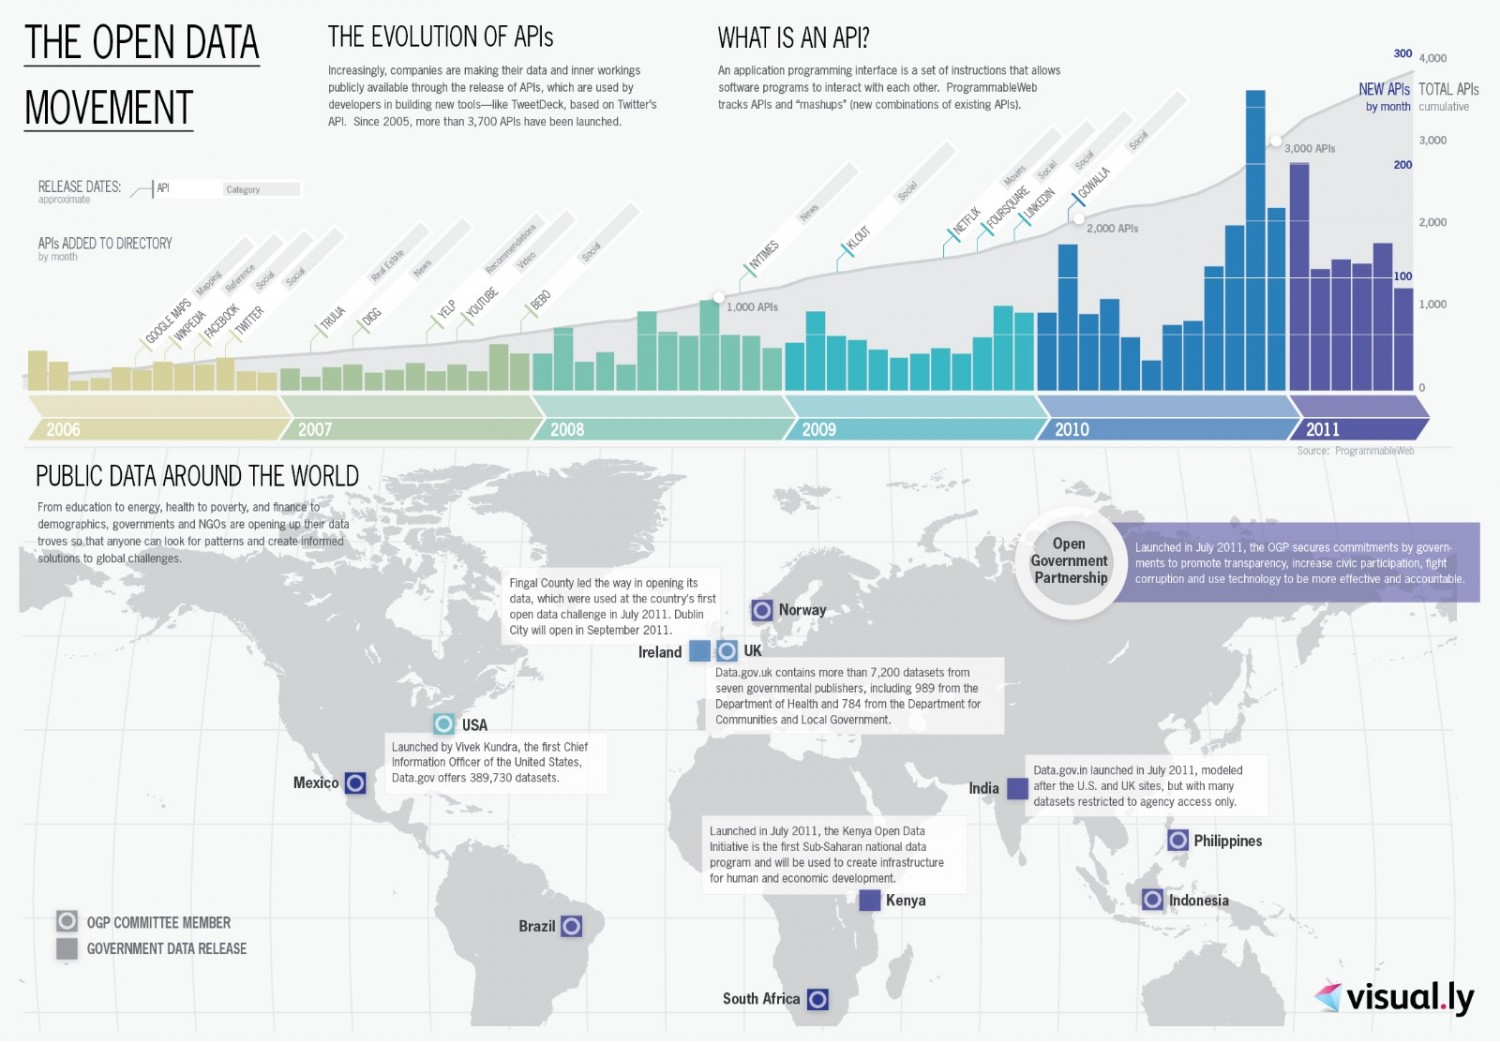
\includegraphics[scale=0.3]{graphics/opendata}
\end{figure}


Se estima que la apertura de datos, solo en Estados Unidos, puede generar entre 3 y 5 billones de dólares \cite{revenueOpenData}. El principal motivo es el gran potencial económico que puede suponer, ya que se podría aumentar la eficiencia en diferentes aspectos de la sociedad, como en la sanidad y educación, además, crearía nuevos servicios y productos, que irían acompañados de puestos de trabajo, y podrían mejorar la percepción para las personas sobre el mundo en general al aumentar la transparencia de la información.

Por otro lado en Europa, otros estudios prevén que el uso de datos abiertos reportará un ahorro de más de 1.7 billones de euros a las administraciones públicas, reducirá en un 16\% la energía consumida y el tiempo de espera en las carreteras. Aparte, indica que las compañías que siguen una filosofía de datos abiertos aumentan su valor en mayor medida que otras que no los abren \cite{valueOpenData}.

Por tanto, se espera que en el futuro cercano más y más países y organizaciones se sumen a estas iniciativas de apertura de datos y, que, los países que ya están participando en ellas, mejoren la calidad de la información que suministran, cuyos formatos, en ocasiones, no pueden ser utilizados sin una transformación a otros adecuados para la lectura por las máquinas.

\begin{figure}[htp!]
\centering
\caption{Valor potencial de los datos abiertos en billones de dólares en Estados Unidos}
\label{fig:revenue}
\vspace{5pt}
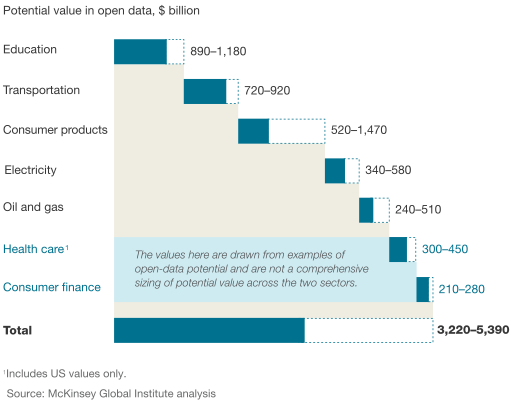
\includegraphics[scale=0.8]{graphics/revenue}
\end{figure}

\newpage
\section{Big Data}
\subsection{Introducción}
El término \textit{big data} es relativamente reciente, su primera aparición parece datar de 1989 cuando Erik Larson lo utilizó en una artículo para la revista Harper's, aunque, se creé que se definió como tal en los años noventa durante las charlas que daba John Mashey, científico jefe de Silicon Graphics, donde explicaba el término para vener sus productos, como se puede ver en presentaciones suyas de 1998 \cite{originbd}.

Sin embargo, los pilares en los que se basa el \textit{big data} no son nada nuevos. Los seres humanos nos hemos caracterizado por la idea de almacenar toda la información posible para crear una base de datos en continúa expansión que pueda ser analizada y de donde se extraiga conocimiento valioso para la humanidad.

Ya en el año 18000 \gls{AC}, había tribus paleolíticas que mediante muescas en palos y huesos hacían seguimientos de las reservas de suministros y de las actividades comerciales, permitiendo hacer predicciones sobre la duración de los alimentos almacenados. También, sobre el año 2400 \gls{AC} surge el ábaco en Babilonia que permitía realizar cálculos.

Como ejemplo de primer almacén de datos, tenemos a la Biblioteca Real de Alejandría, que fue la colección de conocimiento del antiguo mundo. Como primer ejemplo que definió el término ``Business intelligence'', contamos con el banquero Henry Furnese que utilizó en 1985 los datos recolectados de su negocio para obtener una ventaja competitiva frente a sus adversarios.

Pero es durante la segunda mitad del siglo XX y el XXI donde se produce los avances que han permitido llegar a la realidad actual. Hitos como el desarrollo de la computación, los sistemas de almacenamiento digital e Internet y las conexiones inalámbricas han sido las que han permitido crear y almacenar grandes cantidades de datos, unas cantidades que crecen exponencialmente con el tiempo.

\subsection{Definición \label{defBigData}}
Si buscamos la definición de \textit{big data} en Internet podemos encontrar diversas versiones de la misma \cite{ayuso}, algunas más correctas y otras menos, pero no existe un consenso claro sobre el término. Sin embargo, la agencia de la \gls{ONU} encargada de las tecnologías de la  información, creadora del primer estándar \textit{big data} lo define como un paradigma que permite la recolección, almacenamiento, manejo, análisis y visualización de extensos conjuntos de datos, con características heterogéneas y con restricciones de tiempo cercanas al tiempo real \cite{estandar}. 

Otro aspecto que ejemplifica estos cambios en la definición del concepto se puede apreciar en la conocida forma de describir el \textit{big data}, las V's. Estas comenzaron siendo tres \cite{ayuso}, para pasar a ser 4 \cite{4v} y, luego, 5 \cite{monse}, 7 \cite{soriano} e, incluso, 10. En la figura \ref{lasv} se puede apreciar como ha sido este proceso a lo largo del tiempo.

\begin{figure}[htp!]
	\centering
	\caption{Evolución de las V's que definen el \textit{big data} a lo largo del tiempo \cite{fotoV}}
	\label{lasv}
	\vspace{5pt}
	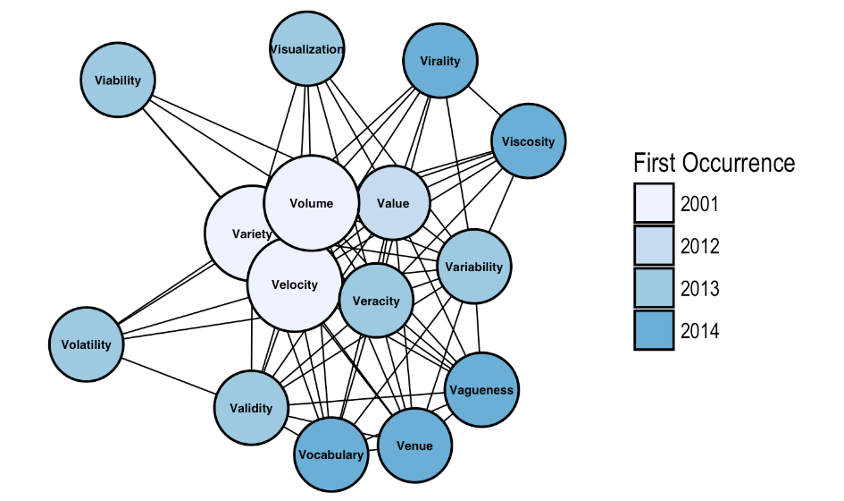
\includegraphics[scale=0.5]{graphics/lasv}
\end{figure}

Aunque, igual que en el caso de la definición, el número de V's variará dependiendo del experto al que consultes, podemos establecer cuatro aspectos básicos de un sistema para que este sea considerado \textit{big data}. Estos son:

\begin{itemize}
\item \textbf{Volumen:} Referido como al tamaño y la cantidad de los datos, aunque no existe un límite establecido ya que estas cantidades cada vez aumentan a un mayor ritmo.
\item \textbf{Velocidad:} Referido a la rapidez con la que se accede a los datos. Lo que se busca en un análisis en tiempo real.
\item \textbf{Variedad:} Referido al número de fuentes diferentes de donde provienen los datos. Los sistemas \textit{big data} tienen que poder procesar datos de diversos orígenes y estructuras.
\item \textbf{Veracidad:} Referido a la certeza de que los datos contenidos en el sistema son reales. Un sistema \textit{big data} debe procurar mantener a cero la información no veraz a razón de no perder eficiencia.
\end{itemize}

\subsection{Propósitos}
Muchas grandes compañías del sector tecnológico llevan años usando herramientas \textit{big data} para mejorar su negocio, compañías pioneras en este campo como Google y Yahoo que desarrollaron primeras versiones de esta tecnología buscando mejorar el resultado de sus buscadores.

Como ya se ha comentado anteriormente, las posibles aplicaciones de estas herramientas son infinitas. En general, disponer de un conjunto de datos que contengan información sobre situaciones pasadas o sobre sucesos y elementos que puedan influenciar un proceso es beneficioso para saber como actuar de la forma más correcta posible.

En general, se pueden encontrar cuatro tipos de usar herramientas \textit{big data} \cite{tipoAnalisis}. Por un lado, podemos encontrar el análisis prescriptivo, que es el más valioso y menos usado, que consiste la utilización de los datos para encontrar posibles caminos de actuación que permitan anticiparse al futuro y obtener ventaja. Un caso donde se está empezando a utilizar este tipo de análisis es en los sistemas de salud, donde conociendo los datos de un grupo, se pueden encontrar patrones para atajar enfermedades de la forma más efectiva.

Otro tipo de análisis es el predictivo, donde se busca detectar patrones que hayan ocurrido en el pasado para predecir el futuro. Este, está siendo especialmente utilizado en los procesos de venta, por ejemplo, para ajustar los precios en base a la oferta y la demanda, así como para preparar los ``stocks'' de los productos.

El análisis de diagnóstico es aquel que busca determinar porque se ha producido algún suceso, usando para ello los datos relacionados con el evento. Este es especialmente utilizado en marketing, para entender el efecto que han tenido las campañas, pero, también en sistemas de software, para conocer el motivo del error y poder evitar situaciones similares en el futuro.

Finalmente, el análisis descriptivo o minería de datos, que busca información valiosa entre todos los datos almacenados. Un ejemplo de este tipo de análisis se da en el estudio de los riesgos al ofrecer un crédito, donde se puede buscar en el pasado financiero del cliente datos que puedan describir la capacidad económica del mismo.

\subsection{Visión de negocio y futuro}
La amplias posibilidades que las herramientas \textit{big data} ofrecen junto con el conocido éxito de empresas y su, cada vez, más sencilla implementación está haciendo que cada vez más y más negocios implementen estas tecnologías.

El ``landscape'' también ha ido creciendo durante estos últimos años, debido al auge de estas tecnologías, haciendo que las herramientas y arquitecturas disponibles haya aumentado, disponiéndose de un amplio abanico de opciones que se adaptan a todo tipos de datos y análisis. En la figura \ref{landscape} se puede observar el panorama actual.

\begin{figure}[htp!]
	\centering
	\caption{Panorama de las tecnologías \textit{big data} en 2017 \cite{landscape}}
	\label{landscape}
	\vspace{5pt}
	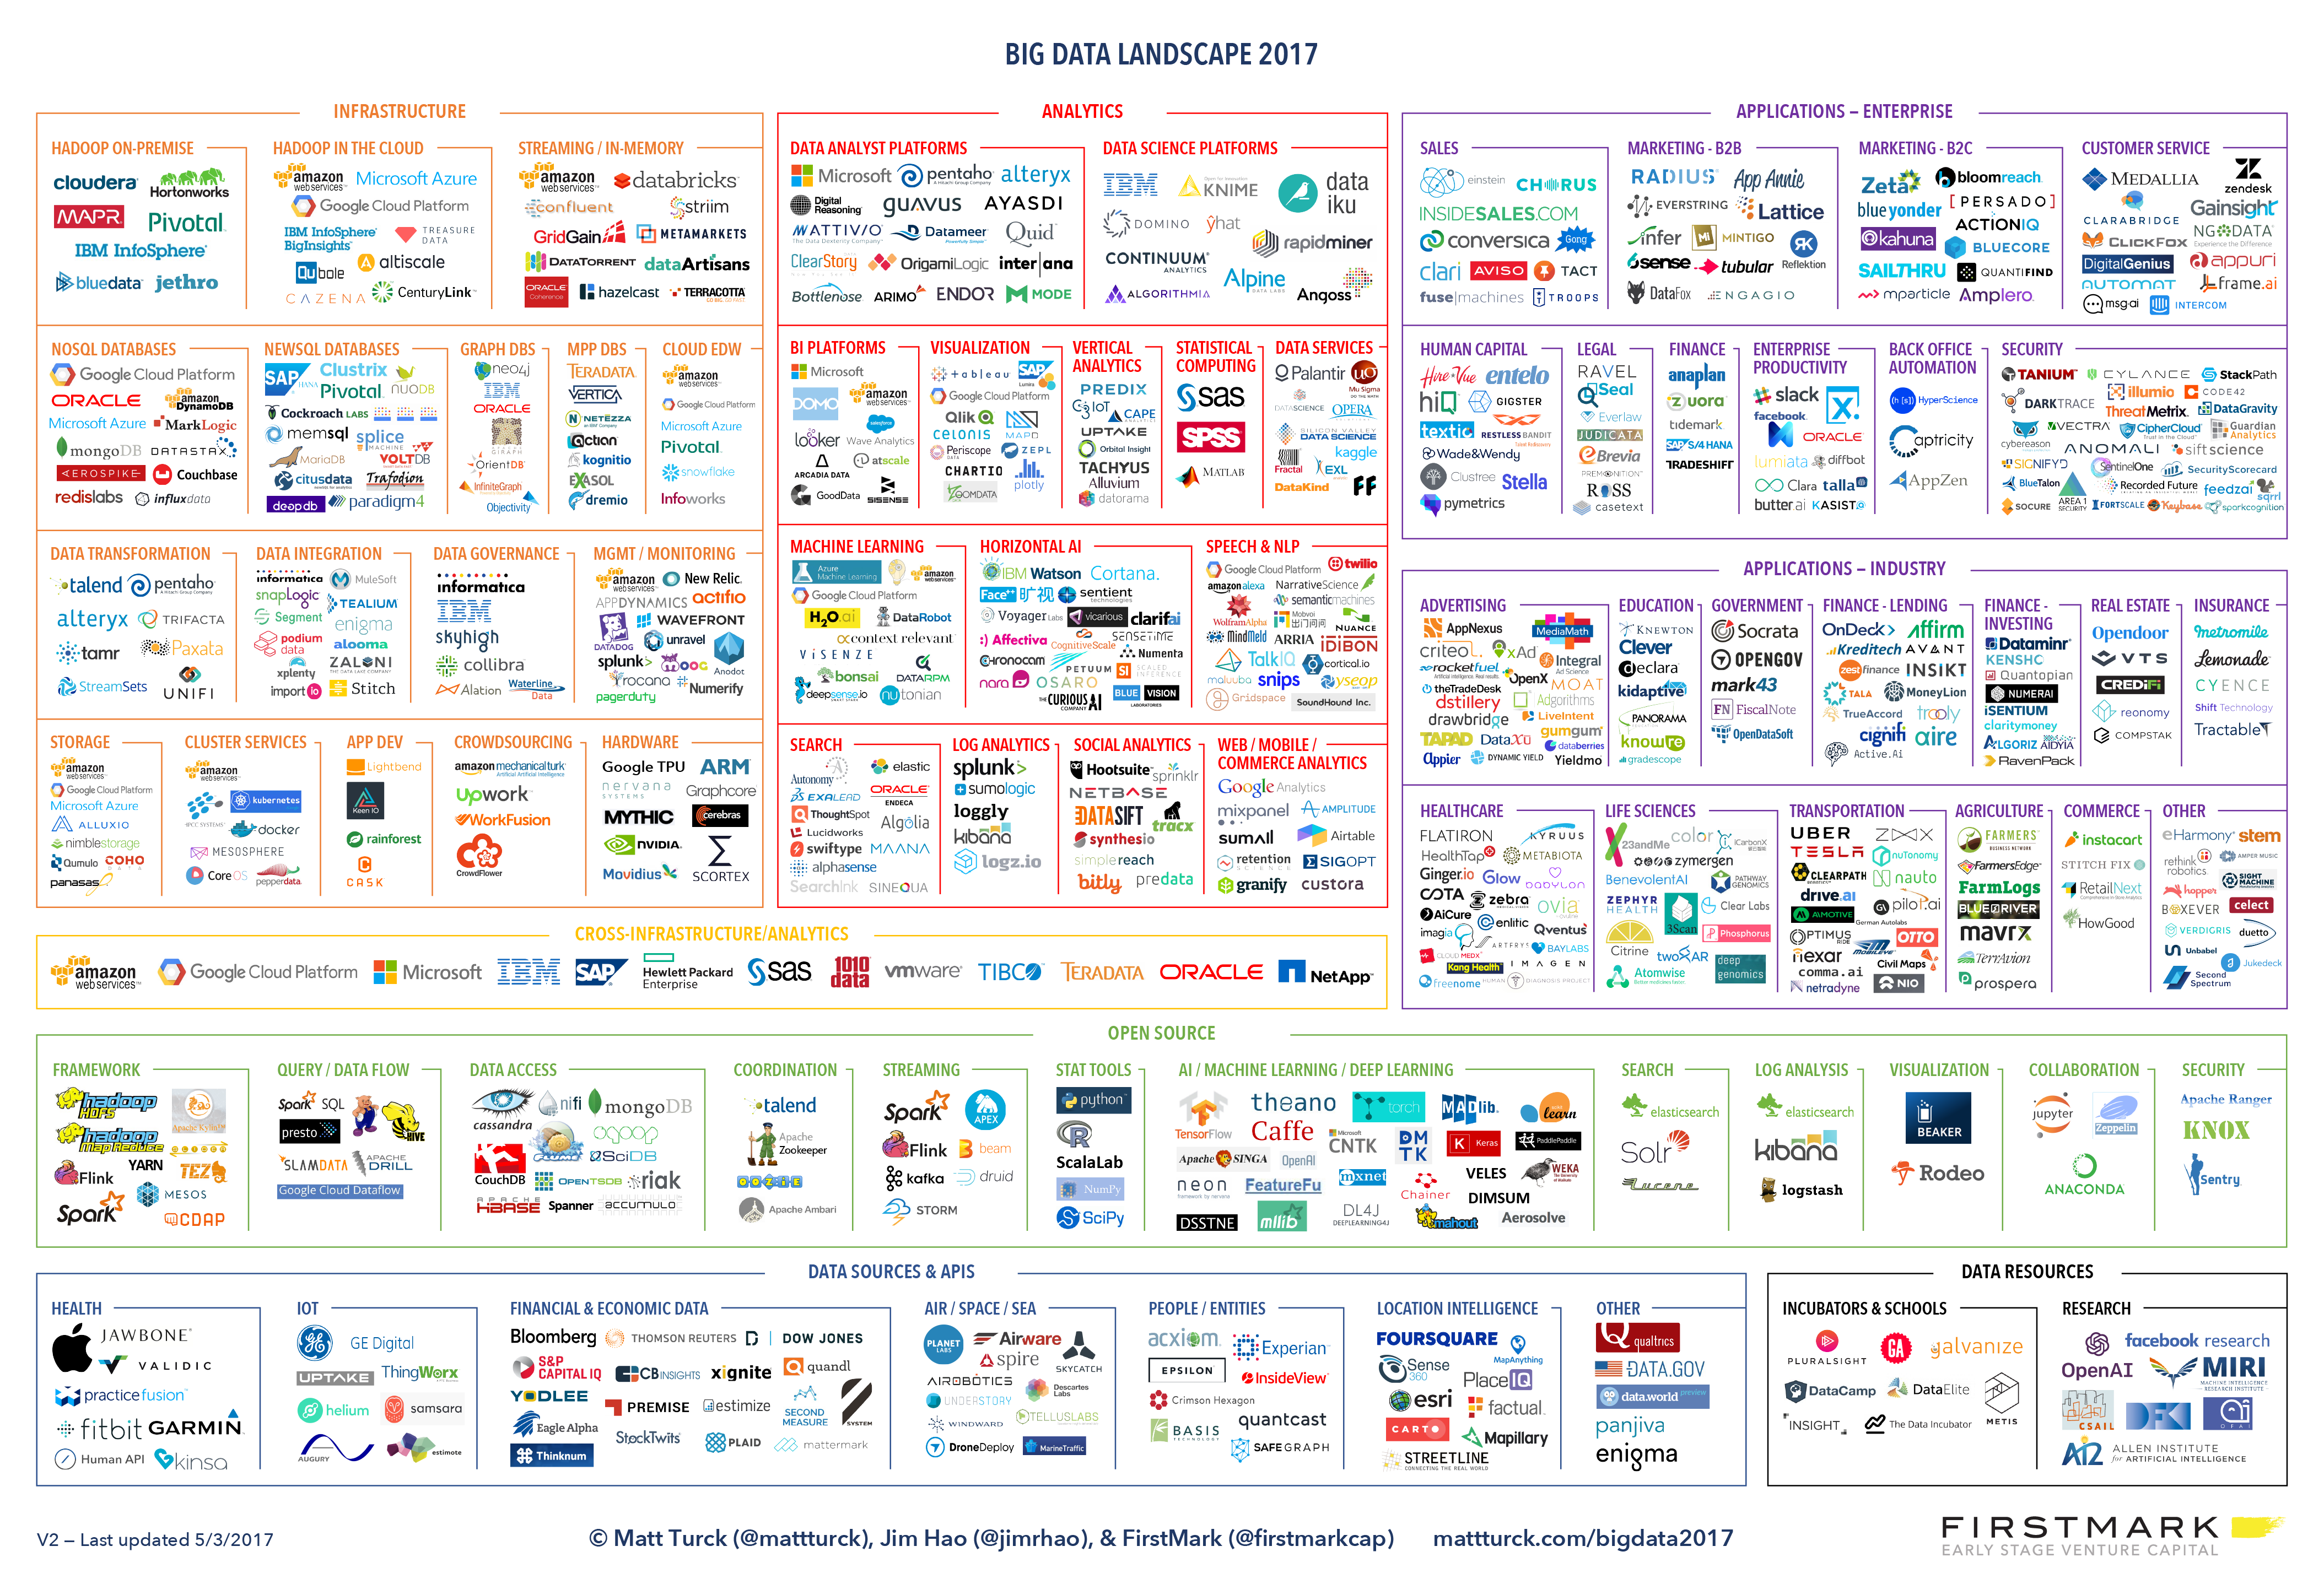
\includegraphics[scale=0.22]{graphics/landscape}
\end{figure}

Una de las características de este paradigma tecnológico es la naturaleza abierta de las herramientas, donde las más usadas son de código abierto y han surgido del resultado de la colaboración de diferentes empresas u organizaciones. Librerías como \textit{Apache Hadoop} \cite{hadoop} o \textit{Apache Spark} \cite{spark}, bases de datos como \textit{Apache Cassandra} \cite{cassandra} o \textit{MongoDB} \cite{mongo} y herramientas de análisis como \textit{SciPy} \cite{scipy} son de uso libre y no requieren de pago de licencias.

Esto ha hecho surgir empresas que se encargan de establecer y mantener un sistema \textit{big data}, es decir, ha permitido a los negocios externalizar este proceso, ahorrándose el presupuesto del diseño y la implantación de estos sistemas. Empresas como Hortonworks \cite{horton}, Cloudera \cite{cloudera} o Databricks \cite{databricks}, ofrecen sistemas de análisis de datos a empresas que utilizan las herramientas mentadas anteriormente, centrando su negocio en el cobro por el uso de recursos computacionales y el servicio técnico.

A este tipo de servicio que ofrecen estos negocios se les conoce como \gls{BDaaS} y se definen como servicios en la nube que permiten al usuario la capacidad de recoger, almacenar, analizar, visualizar y manejar los datos usando \textit{big data}.

El futuro del \textit{big data} parece prometedor, como se puede apreciar en la figura \ref{forecast}, proyectándose un crecimiento del 14.4\% anual en los ingresos generados por el \textit{big data}, pasando de los 18 billones de dólares en 2014 a los 92 en 2022. En general, las estadísticas de crecimiento son muy favorables para este sector tecnológico, con predicciones de entre el 4\% al 15\% \cite{forecast}.

Sin embargo, las tecnologías \textit{big data} no solo mejorarán los resultados económicos de las empresas. Estas, influirán directamente en los usuarios, mejorando las relaciones de estos con los servicios, principalmente, mediante la personalización de estos en base al cliente. También aumentarán la transparencia, al disponerse de más datos, permitiendo al usuario tener más conocimiento sobre las opciones disponibles.

\begin{figure}[htp!]
	\centering
	\caption{Proyección de los ingresos del \textit{big data}  \cite{forecast}}
	\label{forecast}
	\vspace{5pt}
	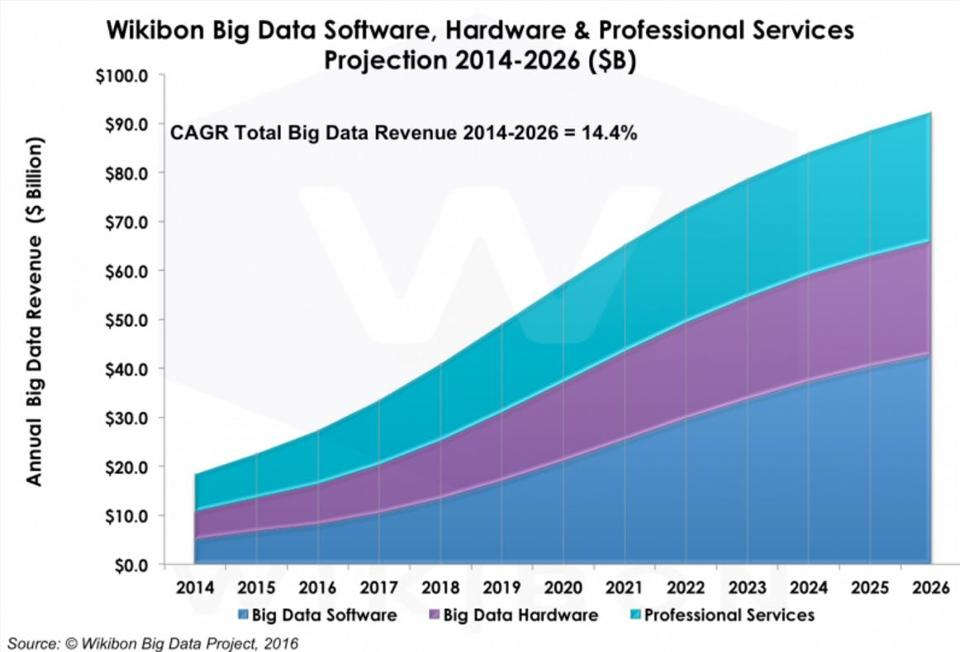
\includegraphics[scale=0.5]{graphics/forecast}
\end{figure}

\section{Sistemas distribuidos}
La computación distribuida es un modelo de computación que consiste en la conexión de diferentes máquinas, que pueden estar en localizaciones físicas distintas, con el fin de realizar tareas en un tiempo menor del que necesitaría una sola máquina. Es decir, un sistema distribuido es una red de equipos autónomos que se comunican entre ellos para conseguir un objetivo. Estos son independientes en el sentido que no comparten memoria o procesadores físicamente \cite{computacionDistribuidad}.

Estos ordenadores se comunican entre ellos por ``mensajes'' que son fragmentos de información que se intercambian por la red. Estos mensajes sirven para ordenar diferentes tareas con argumentos particulares, para enviar y recibir paquetes de datos o para mandar ordenar comportamientos específicos de otros ordenadores. Estas máquinas pueden tener diferentes roles dentro del sistema, dependiendo de su objetivo. 

\begin{figure}[htp!]
	\centering
	\caption{Esquema computación distribuida \cite{fotodistribuida}}
	\label{distribuida}
	\vspace{5pt}
	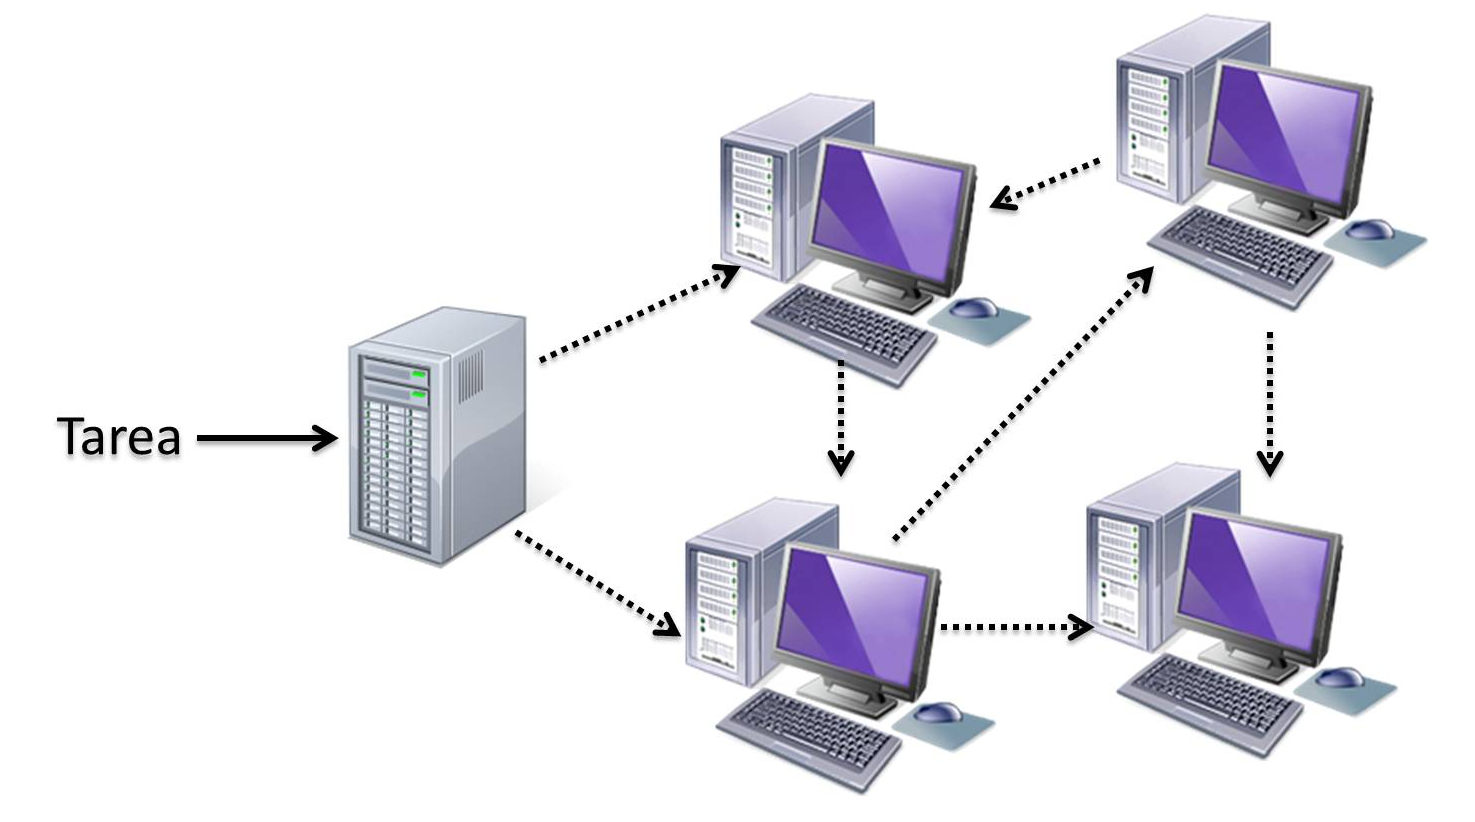
\includegraphics[scale=0.3]{graphics/computaciondistribuida}
\end{figure}

Las ventajas que ofrece este tipo de computación son \cite{sistDistTeoria}:

\begin{itemize}
\item \textbf{Compartición de recursos:} Este modelo de computación permite que las máquinas compartan recursos de hardware al estar conectadas en red.

\item \textbf{Escalabilidad:} Gracias a la capacidad de compartir recursos, nuevos sistemas pueden ser añadidos a la red y aumentar la capacidad del conjunto.

\item \textbf{Tolerancia a fallos:} Al contarse con varias máquinas, la caída de alguna de ellas de la red no será crítico, permitiendo la continuidad del sistema.

\item \textbf{Concurrencia:} Este modelo permite que se ejecuten varios procesos al mismo tiempo dentro de la red.

\item \textbf{Variedad:} Se pueden incorporar máquinas con diferente hardware y software debido al uso de protocolos estándar.
\end{itemize}

A pesar de estas ventajas, también cuenta con inconvenientes como los siguientes:

\begin{itemize}
\item \textbf{Complejidad:} Por el hecho de que se cuenta con varias máquinas, la organización y control de estos sistemas es más complicado que el de una sola máquina.

\item \textbf{Seguridad:} Debido a que existen conexiones remotas que conectan a los equipos del sistema, se puede dar el caso de escuchas e interceptación de mensajes.

\item \textbf{Disparidad en el comportamiento:} Se puede dar el caso de obtención de resultados diferentes dependiendo de las condiciones.
\end{itemize}

\subsection{Configuraciones}
Existen dos arquitecturas predominantes para la creación de sistemas distribuidos, la configuración cliente-servidor y la ``peer-to-peer''.

\subsubsection{Cliente-servidor}
La arquitectura cliente-servidor es una forma de ofrecer servicios desde una fuente central, es decir, existe un solo servidor a los que múltiples clientes se conectan para consumir sus productos. 

\begin{figure}[htp!]
	\centering
	\caption{Esquema cliente-servidor  \cite{computacionDistribuidad}}
	\label{clientserver}
	\vspace{5pt}
	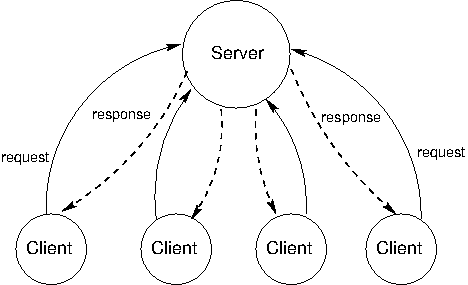
\includegraphics[scale=0.6]{graphics/clientserver}
\end{figure}

En este tipo los roles de los equipos son diferentes, mientras que el servidor es responder a las peticiones de los clientes, el trabajo de los clientes es usar los datos recibidos desde el servidor para realizar alguna tarea.

Internet es un ejemplo muy importante de este tipo de arquitectura ya que esta basada en ella, donde el servidor es una máquina que ofrece la página web a los sistemas que se conectan con ella. Sin embargo este sistema tiene dos importantes inconvenientes, por un lado, si se cae el servidor se paraliza el servicio totalmente. Por otro, este modelo no tiene capacidad de escalar, por lo que cuando hay muchos clientes conectados el rendimiento disminuye.

\subsubsection{Peer-to-peer}
Son aquellos sistemas distribuidos en los que el trabajo está dividido entre todos los componentes del sistema. Todos las máquinas envían y reciben datos y aportan capacidad de computación y memoria al sistema, siendo este más potente cuanto más integrantes tenga la arquitectura.

\begin{figure}[htp!]
	\centering
	\caption{Esquema peer-to-peer \cite{peertopeer}}
	\label{peertopeer}
	\vspace{5pt}
	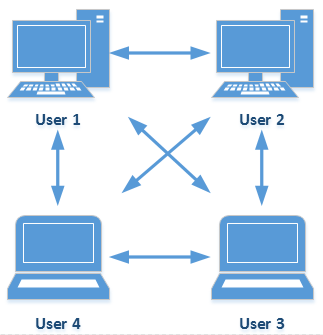
\includegraphics[scale=0.6]{graphics/peertopeer}
\end{figure}

La división del trabajo entre todos las máquinas es el aspecto clave de esta arquitectura y, para mantenerla, mantener un comunicación fiable es básico. Por ello, para asegurar que los mensajes llegan entre los componentes, la red de un sistema peer-to-peer es estructurada y todos los nodos del mismo tienen que procurar en tener suficiente información de la misma para mantenerlo.

Existen variaciones de este sistema donde hay elementos que se preocupan de mantener la conexión entre todos los equipos de la red, de controlar la información del sistema y proporcionarla y organizar las tareas del conjunto. Este tipo de sistema es el que utilizaremos en este proyecto, donde habrá un maestro que organizará las tareas y los esclavos que realizarán el procesamiento.

Las aplicaciones más comunes de este tipo de arquitecturas son la transferencia de datos y almacenamiento. También aplicaciones como Skype funcionan con esta tecnología.

\subsection{Arquitectura utilizada}
Como hemos comentado anteriormente, en este proyecto vamos a usar una variación de la arquitectura de sistemas distribuidos peer-to-peer, donde tendremos una máquina que hará de maestro y será la que se encargue de establecer la conexión con el resto de elementos, repartir las tareas y recolectar los datos. El resto hará de esclavos de esta máquina, realizando las tareas encargadas.

En este caso, además utilizaremos dos configuraciones de esta arquitectura, un modo pseudo-distribuido y otro distribuido o multinodo.

\subsubsection{Pseudo-distribuido}
En esta configuración se contará con una sola máquina que hará de maestro y esclavo. Es decir, en este modo, habrá un proceso en el equipo que ordene a otro conjunto de procesos que harán de esclavos y realizarán el trabajo.

El objetivo de este sistema es establecer una base con la que comparar el resto de configuraciones, es decir, al ser una única máquina sus resultados de tiempo y eficiencia deberían ser los peores, estableciendo un umbral mínimo.

\subsubsection{Clúster o multinodo}
Un clúster es un conjunto de ordenadores conectados entre sí por una red de alta velocidad y que se comportan como si fueran un único sistema \cite{cluster}. 

\begin{figure}[htp!]
	\centering
	\caption{Esquema de un clúster \cite{clusterfoto}}
	\label{clusterDef}
	\vspace{5pt}
	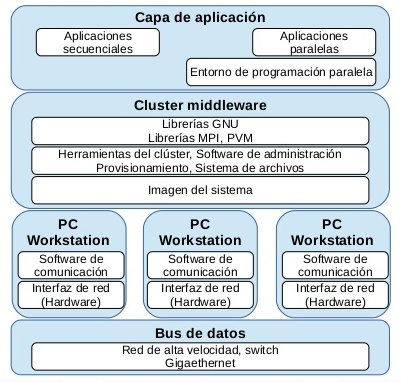
\includegraphics[scale=0.7]{graphics/clusterDef}
\end{figure}

La tecnología de clústeres es usada en tareas de cómputos o supercómputos, en servidores web y comercio electrónico y en bases de datos de alta disponibilidad. Es decir, las características de que se esperan de un clúster son las siguientes \cite{cluster}:

\begin{itemize}
\item \textbf{Alto rendimiento:} Debido a que se trata de un conjunto de ordenadores, la suma de su potencia hace que sean óptimos para tareas que requieran gran capacidad de computación y sean paralelizables. 

\item \textbf{Alta disponibilidad:} Por la misma razón, los clústeres deben ofrecer una rápida capacidad de recuperación ante fallos, por ejemplo, pudiendo recuperar los datos de un nodo perdido al guardar copias en otros o evitando la caída del sistema por el fallo en un nodo, siendo este sustituido.

\item \textbf{Balanceo de carga:} Un clúster debe distribuir el trabajo entre todos los nodos de la manera más equilibrada posible.

\item \textbf{Escalabilidad:} El sistema tendría que tener facilidad para adaptarse a las diferentes situaciones, siendo posible añadir o reducir capacidad del sistema mediante la adición o extracción de nodos del mismo.
\end{itemize}

Los elementos de un clúster son:

\begin{itemize}
\item \textbf{Bus de datos:} Que conecta a los nodos del clúster y permite la comunicación entre ellos.

\item \textbf{Nodos:} Es el conjunto de máquinas que forman el clúster, todas ellas tendrán que estar conectadas a la red y disponer de un software, el \gls{SO} que deberá ser multiproceso y multiusuario.

\item \textbf{Middleware:} Que permitirá el entendimiento entre las aplicaciones y el sistema operativo de los nodos. Es el encargado de hacer que el clúster sea visto por el usuario como una única entidad y, por otro lado, es el encargado de realizar el balanceo de tareas y permitir la escalabilidad del sistema.
\end{itemize}

\clearpage
\section{Infraestructura}
\subsection{Apache Spark \label{sparkEA}}
\textit{Apache Spark} \cite{spark} es un \gls{framework} de código abierto que permite el procesamiento de datos mediante la computación distribuida. Desarrollado originalmente por el departamento AMPLab de la Universidad de California, fue, posteriormente, donado a la fundación Apache, que lo ha mantenido desde entonces. 

Desarrollado en Scala \cite{scala} y con soporte para Java, Python y R, \textit{Apache Spark} proporciona una \gls{API} para programar clúster con paralelismo de datos implícito y tolerancia a fallos. Esta \gls{API} se apoya en la estructura llamada \gls{RDD}, donde se almacenan los datos particionados para permitir transformaciones en paralelo y que mantiene el índice de estas transformaciones para rehacerlas en caso de error.

Una buena característica de este \gls{framework} es el amplio soporte para la mayoría de los formatos de ficheros de datos, teniendo, además, integraciones con varios sistemas de almacenamiento como \gls{HDFS}, \textit{Apache Cassandra} \cite{cassandra} o Amazon S3 \cite{aws}. En la figura \ref{partSpark} podemos observar los diferentes componentes que conforman \textit{Apache Spark}.

\begin{figure}[htp!]
	\centering
	\caption{Componentes de \textit{Apache Spark} \cite{partsSpark}}
	\label{partSpark}
	\vspace{5pt}
	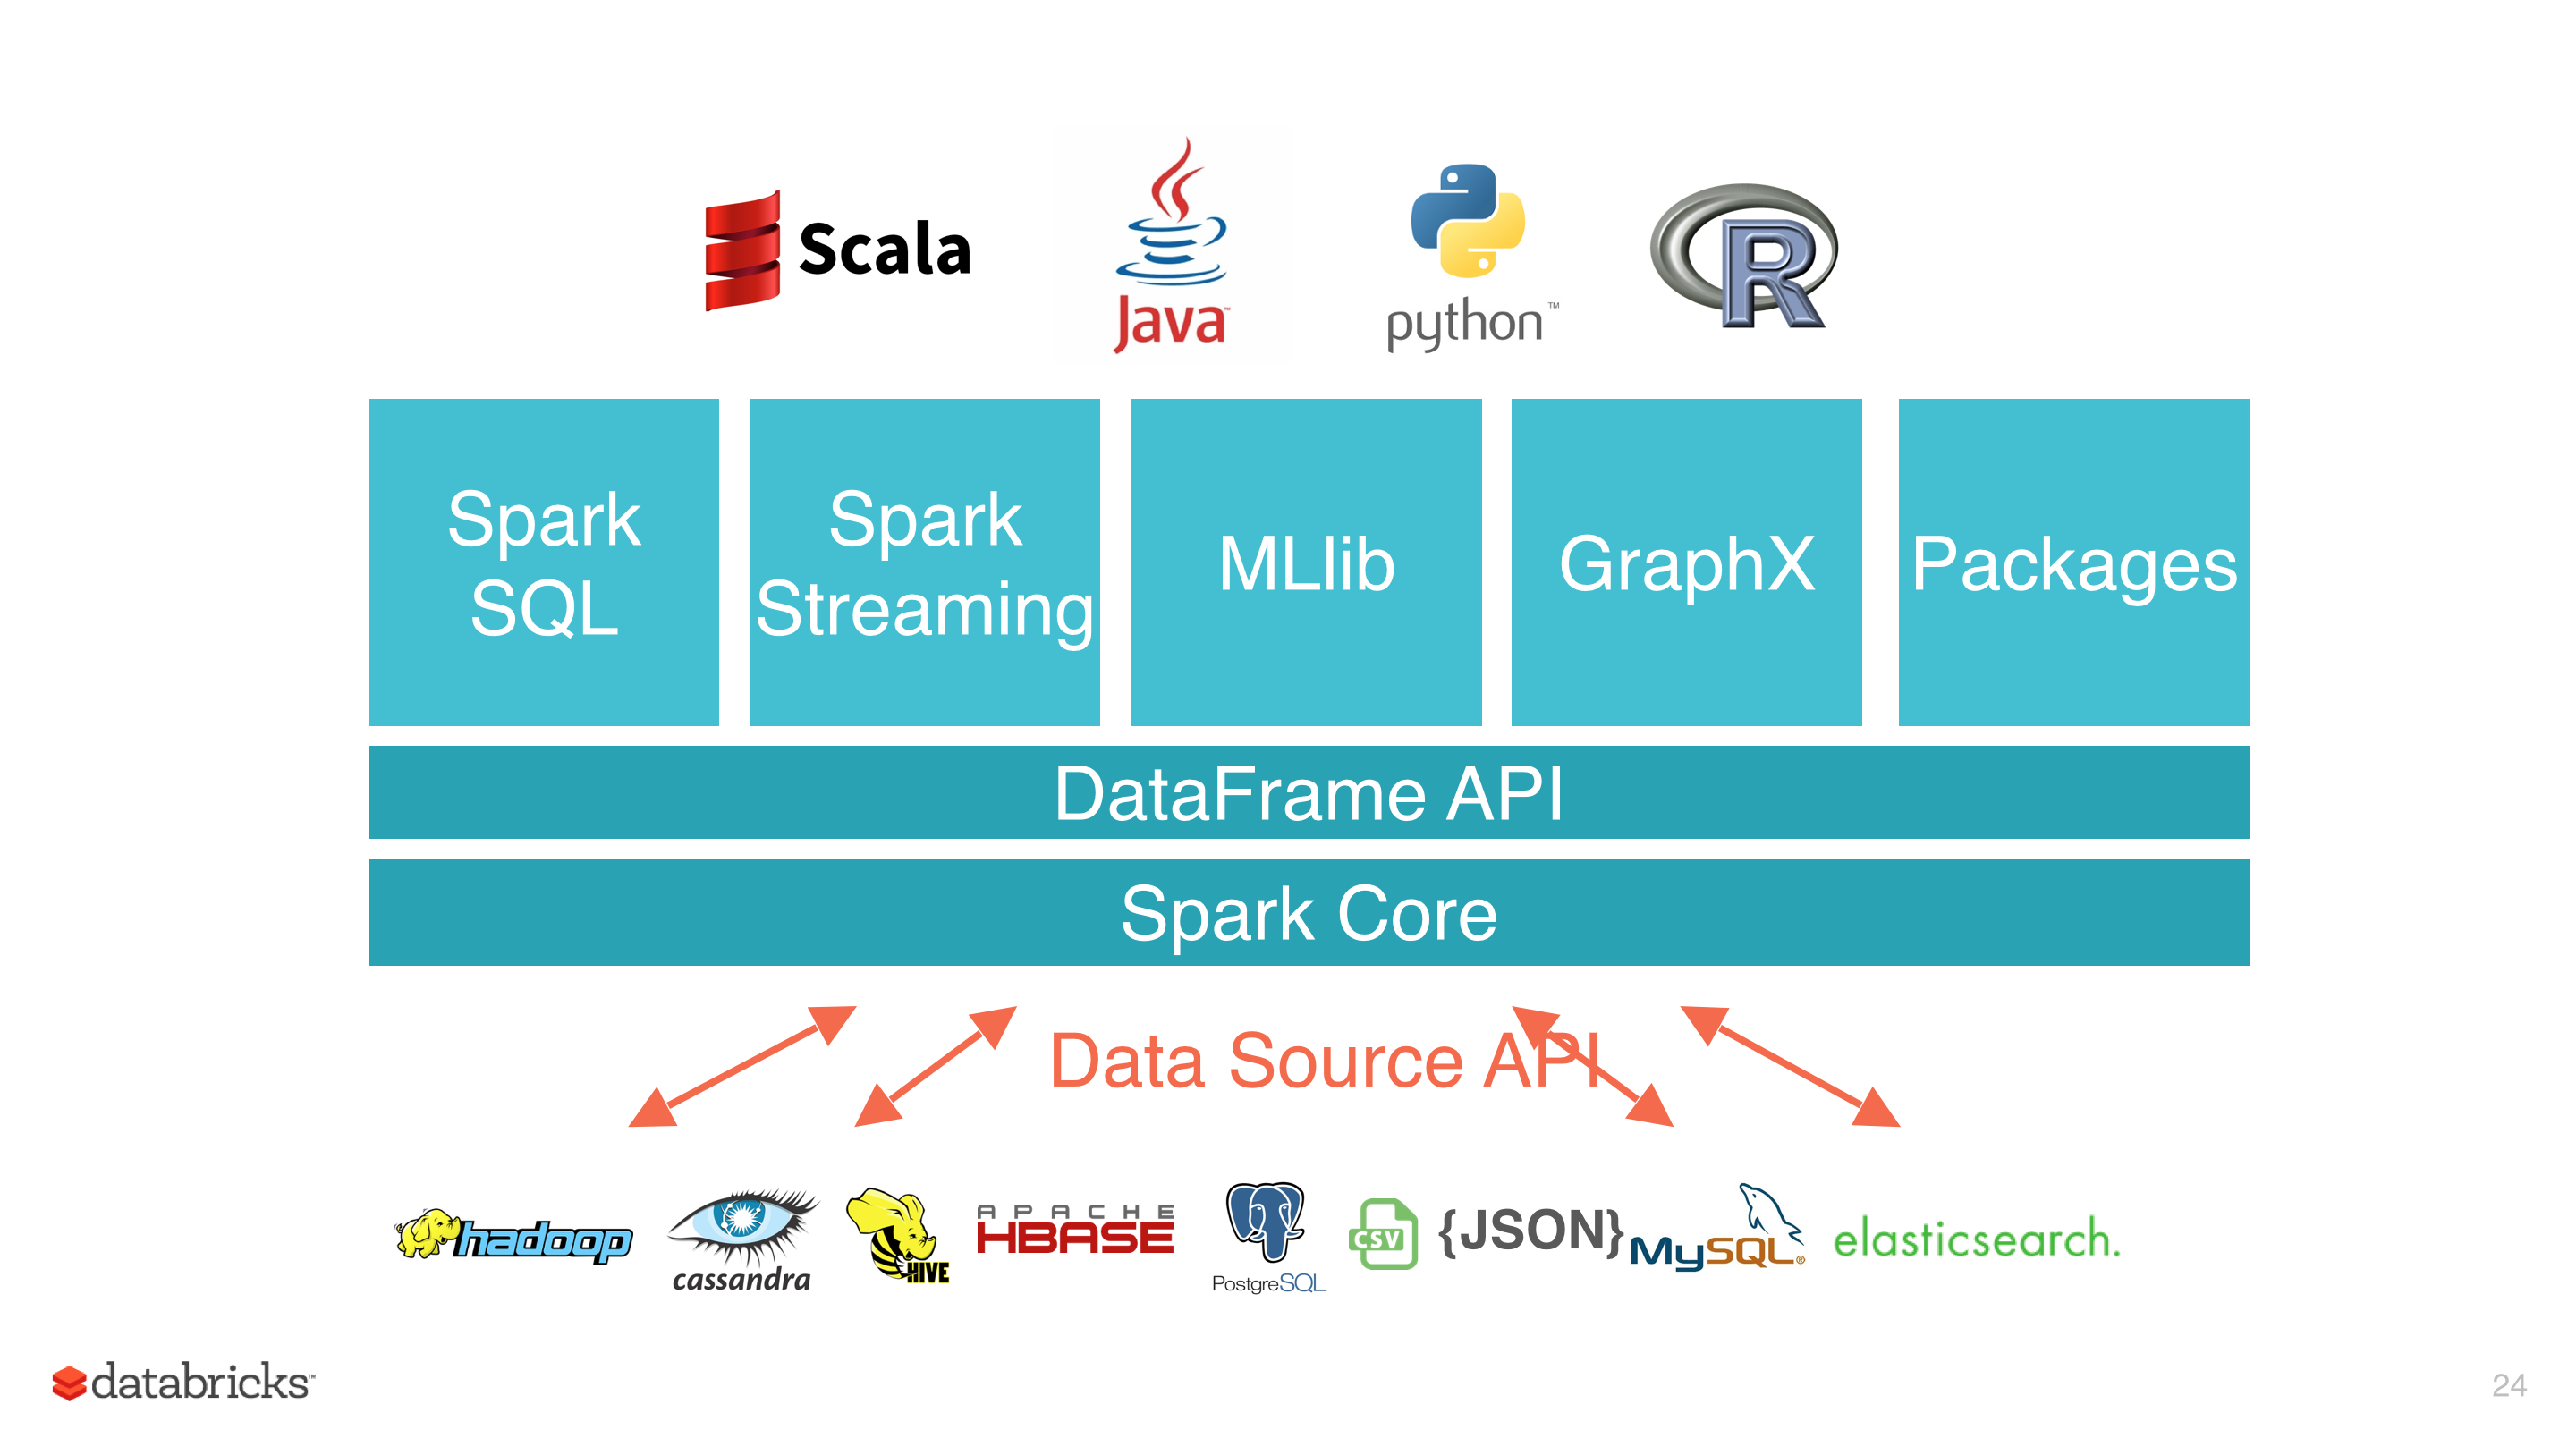
\includegraphics[scale=0.31]{graphics/partSpark}
\end{figure}

El \gls{framework} está formado por una base, sobre la que trabajan las diferentes librerías y paquetes del mismo. Dicha base está formada por el núcleo del programa, donde se crean y manipulan los \gls{RDD}, y la DataFrame API, que es una abstracción a más alto nivel de los \gls{RDD}, para simplificar su manipulación por el usuario.

Además \textit{Apache Spark} cuenta con diversas librerías como Spark SQL, para realizar consultas sobre los datos, Spark Streaming, para permitir la introducción y análisis de datos en tiempo real, MLib, para realizar aprendizaje automático, y Graphx, que permite la computación de grafos.

\subsubsection{Funcionamiento}
\textit{Apache Spark} basa su funcionamiento en dos conceptos, \gls{RDD} y \gls{DAG}. Una aplicación consiste en un controlador, llamado \textit{SparkContext}, que utiliza el código de usuario para crear y transformar \gls{RDD} y alcanzar el objetivo final. Estas transformaciones de los \gls{RDD}s son traducidos a gráficos \gls{DAG} para ser enviados al planificador y que este reparta las tareas.

\begin{figure}[htp!]
	\centering
	\caption{Funcionamiento de \textit{Apache Spark} \cite{partsSpark}}
	\label{sparkWork}
	\vspace{5pt}
	\includegraphics[scale=0.35]{graphics/sparkWork}
\end{figure}

\paragraph{\gls{RDD}: Resilient Distributed Dataset}
Esta será la solución utilizada en \textit{Apache Spark} para tratar los datos de una forma paralela y a prueba de errores. Además ofrece diferentes \gls{API}s para realizar transformaciones sobre los datos y permite el control sobre el modo de particionar los datos y el caché de los mismos.

Un \gls{RDD} puede ser creado a partir de un fichero en un almacenamiento externo o a partir de otro \gls{RDD} y es un sistema vago (\textit{lazy}), es decir, se guardan las operaciones que se realizarán sobre los datos, pero estas no son ejecutadas hasta que no se realiza la evaluación de los datos. Este sistema también es utilizado para la evitar los errores, donde el sistema sigue los pasos realizados desde el inicio para recomponer los datos correctamente.

Existen diferentes grupos de operaciones que se pueden realizar sobre un \gls{RDD}, estos son:

\begin{itemize}
\item \textbf{Transformaciones:} Permite realizar las funciones codificadas por el usuario sobre todos los datos del sistema, permite operaciones de agrupación, ordenamiento y particionamiento del \gls{RDD}. Estas operaciones son reflejadas en el grafo \gls{DAG}.

\item \textbf{Acciones:} Son las que inician el trabajo, es decir, hacen que se ejecuten las transformaciones estables

\item \textbf{Persistencia:} Permiten almacenar el \gls{RDD} en memoria o en disco de forma explicita.
\end{itemize}

\paragraph{\gls{DAG}: Direct Acyclic Graph} 
Es la forma de codificación de los trabajos sobre los \gls{RDD}s utilizada en \textit{Apache Spark}. Indica el flujo que seguirá la aplicación durante la ejecución que, generalmente, se basa en leer los datos del origen, realizar las transformaciones oportunas y materializar los datos obtenidos.

\begin{figure}[htp!]
	\centering
	\caption{Transformaciones sobre un \gls{RDD} representadas en un \gls{DAG} \cite{partsSpark}}
	\label{dag}
	\vspace{5pt}
	\includegraphics[scale=0.4]{graphics/dag}
\end{figure}

Este componente también es el que se encarga de establecer las diferentes tareas del trabajo que, posteriormente, serán repartidas entre los nodos del clúster para paralelizar el trabajo.

Una de las características que diferencia \textit{Apache Spark} es la forma en la que gestiona los datos, este \gls{framework} guarda los datos en la memoria \gls{RAM} del dispositivo, sin llegar escribir a disco, por lo que el acceso a estos es muy rápido. Por ello, hace que la velocidad en procesos iterativos, donde se consultan los mismos datos de forma continua, sea muy elevada, mejorando con creces los tiempos de otros sistemas como MapReduce \cite{compSpark}.

\begin{figure}[htp!]
	\centering
	\caption{\gls{RDD} distribuido en diferentes máquinas \cite{sparkbook}}
	\label{rdddistribuido}
	\vspace{5pt}
	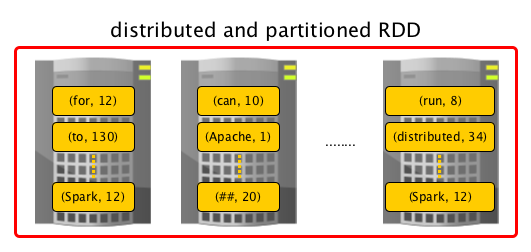
\includegraphics[scale=0.6]{graphics/rdddistribuido}
\end{figure}

\subsubsection{Librerías}
Como se ha indicado anteriormente, \textit{Apache Spark} incluye diferentes librerías que trabajan sobre la base del \gls{framework}. Estas son:

\begin{itemize}
\item \textbf{Spark SQL:} Permite el soporte para datos estructurados o semi-estructurados para realizar consultas \gls{SQL} sobre ellos. Estos datos pueden ser modificados con funciones específicas de \textit{Apache Spark} o mediante el lenguaje \gls{SQL}.

\item \textbf{Spark Streaming:} Permite el análisis en tiempo real de datos mediante la introducción de estos en mini lotes de datos. Este sistema aunque cumple su función no es tan potente como el ofrecido por otras alternativas como \textit{Apache Flink} \cite{flink} o \textit{Apache Storm} \cite{storm}.

\item \textbf{MLib:} Es un \gls{framework} de aprendizaje automático distribuido. Este permite diferente tipos de análisis sobre los datos: clasificaciones, regresiones, clusterizaciones, optimizaciones, etc.

\item \textbf{GraphX:} Es un procesador de grafos distribuido. Es muy veloz para grafos que no tienen que ser actualizados, sin embargo, debido a la naturaleza inmutable de los \gls{RDD} no es una herramienta válida para grafos que se modifiquen.
\end{itemize}

\subsection{Apache Hadoop}
\textit{Apache Hadoop} \cite{hadoop} es otro \gls{framework} de código abierto que permite el tratamiento de grandes cantidades de datos de forma distribuida. Desarrollado en Java, permite la gestión de clústeres de un nodo hasta cientos de ellos de forma sencilla. Al establecer sistemas distribuidos estos tienen una alta tolerancia a los fallos.

\textit{Apache Hadoop} cuenta con cuatro módulos principales, aunque cuenta con muchos más proyectos totalmente compatibles: 

\begin{itemize}
\item \textbf{Hadoop Common:} Utilidades comunes que soportan el resto de módulos.

\item \textbf{Hadoop Distributed File System (\gls{HDFS})} Sistema de ficheros distribuido que permite la replicación de los datos en los nodos del sistema.

\item \textbf{Hadoop YARN:} Es un \gls{framework} que se encarga de la gestión de los trabajos y los recursos del clúster.

\item \textbf{Hadoop Mapreduce:} Sistema basado en YARN para el procesamiento paralelo de grandes cantidades de datos.
\end{itemize}

En este proyecto, debido a que utilizamos \textit{Apache Spark} para la gestión del clúster, no utilizaremos la mayoría de los módulos de \textit{Apache Hadoop}. El módulo que se utilizará será el sistema de ficheros \gls{HDFS} por la configuración distribuida del clúster doméstico. 

Con este sistema realizaremos la replicación de los ficheros de datos en los diferentes nodos del sistema y, de esa forma, ahorrar la transmisión de estos durante la ejecución de los trabajos y, así, mejorar los tiempos de procesamiento.

\subsubsection{Hadoop Distributed File System (\gls{HDFS})}
\gls{HDFS} es un sistema de ficheros distribuido, escalable y portable escrito en Java. Este permite el almacenado de grandes cantidades de datos mediante la distribución de estos en diferentes máquinas. \gls{HDFS} es muy tolerante a los fallos y esta diseñado para correr en hardware de bajo coste. 

\gls{HDFS} fue construido con las siguientes asunciones y objetivos:

\begin{itemize}
\item \textbf{Errores de hardware:} Los fallos de hardware son más una norma que una excepción en la realidad, por ello, \gls{HDFS} es muy tolerante a los fallos, distribuyendo y replicando los datos en diferentes máquinas del clúster para no perder el acceso a ellos por la caída de algún nodo.

\item \textbf{Acceso al streaming de datos:} \gls{HDFS} fue concebido para aplicaciones que necesitan un buen rendimiento en el acceso a los datos, más que para su manipulación continua por los usuarios. Por ello, se centra más en el procesamiento en lotes.

\item \textbf{Grandes volúmenes de datos:} \gls{HDFS} está afinado para manejar ficheros de datos que van desde los cientos de gigasbytes hasta terabytes de tamaño.

\item \textbf{Modelo de coherencia simple:} Las aplicaciones que usan este sistema necesitan el acceso a la lectura del fichero más que sus modificaciones. Por ello, el sistema del \gls{HDFS} usa un modelo ``escribe una vez y lee el resto'', por lo que una vez que se crea un fichero, se escribe y guarda, este no vuelve a modificarse excepto para reducir la cantidad de datos o añadir más.

\item \textbf{``Mover la capacidad de computación es más barato que mover los datos'':} Una aplicación es más eficiente si la computación se realiza cerca de los datos, ya que ahorras el tiempo de transporte de estos. Esta es la premisa que sigue \gls{HDFS} y por ello se replican los datos en todos los sistemas para realizar las operaciones sobre estos en los propios nodos.

\item \textbf{``Portabilidad entre hardware y software heterogéneo: } \gls{HDFS} ha sido diseñado para ser fácilmente portado entre sistemas y plataformas.
\end{itemize}

\begin{figure}[htp!]
	\centering
	\caption{Arquitectura del \gls{HDFS} \cite{hadoop}}
	\label{hdfsarchitecture}
	\vspace{5pt}
	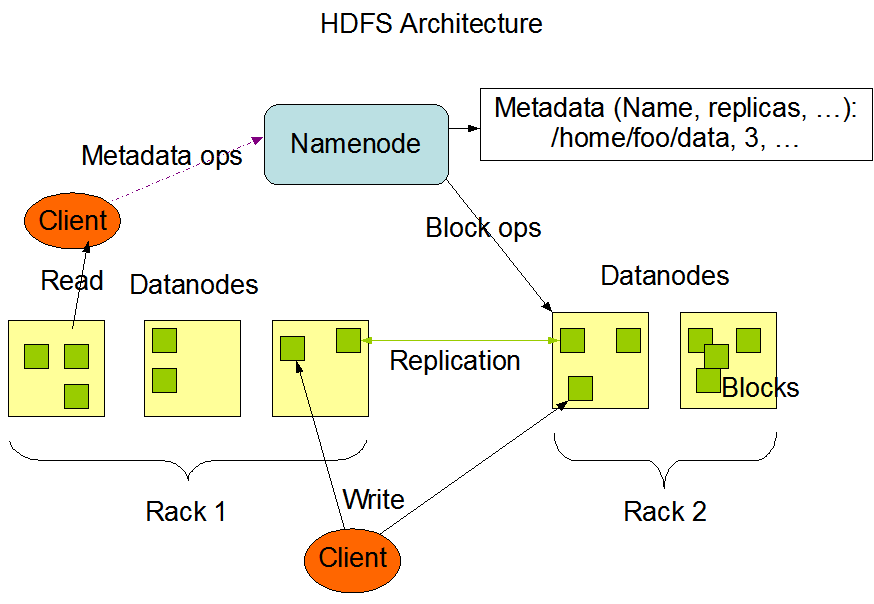
\includegraphics[scale=0.6]{graphics/hdfsarchitecture}
\end{figure}

En la figura \ref{hdfsarchitecture} podemos ver la arquitectura de un sistema \gls{HDFS}, este esta basado en la estructura maestro/esclavo, donde existe una \textit{Namenode} que hace de maestro y gestiona el sistema de ficheros y regula el acceso a los ficheros por los clientes. Por otro lado, están los \textit{Datanodes}, uno por nodo, que es donde se almacenan y gestionan los datos del sistema.

Por otro lado, dentro de estos \textit{Datanodes} encontramos los bloques, que son partes o fragmentos de los datos originales y que se replican por los diferentes nodos.

\subsection{Apache Parquet \label{parquetBeneficios}}
\textit{Apache Parquet} es un formato de fichero de código abierto basado en el almacenamiento columnar. Este es compatible con la mayoría de los \gls{framework}s del ecosistema Hadoop y con \textit{Apache Spark} y ofrece sistemas de compresión y codificación eficientes para mejorar su eficiencia.

\begin{figure}[htp!]
	\centering
	\caption{Comparación entre almacenamiento columnar y basado en filas \cite{column}}
	\label{column}
	\vspace{5pt}
	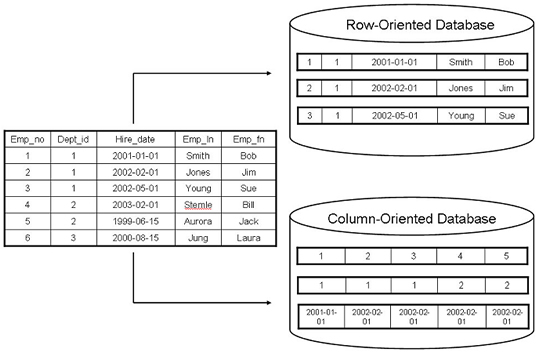
\includegraphics[scale=0.7]{graphics/column}
\end{figure}

El almacenamiento columnar es un modelo en el que la tabla se guarda por columnas en vez de por filas, es decir, lo que se guarda es el conjunto de los datos de una columna y se establece una identificación para saber a que elemento pertenecen los datos. Este modelo es más rápido en muchos casos ya que se puede acceder directamente al atributo deseado, sin tener que descartar el resto de la fila \cite{column}.

Por otro lado, este tipo de almacenamiento es mejor en cuanto al ahorro de espacio debido a que su estructura es más fácil de comprimir, por ejemplo, no es necesario indicar el tipo de cada valor, ya que son todos del mismo tipo al tratarse de la misma columna de la tabla. 

Otra ventaja se aporta cuando los valores de la columna se repiten, ya que este se guarda una vez y se establece las posiciones en las que ocurre. También usa una codificación mínima para los enteros pequeños y permite el trabajo de los datos con aplicaciones de vectorización.

\begin{figure}[htp!]
	\centering
	\caption{Espacio ocupado en disco de un archivo por diferentes formatos \cite{parquetSpace}}
	\label{parquetSpace}
	\vspace{5pt}
	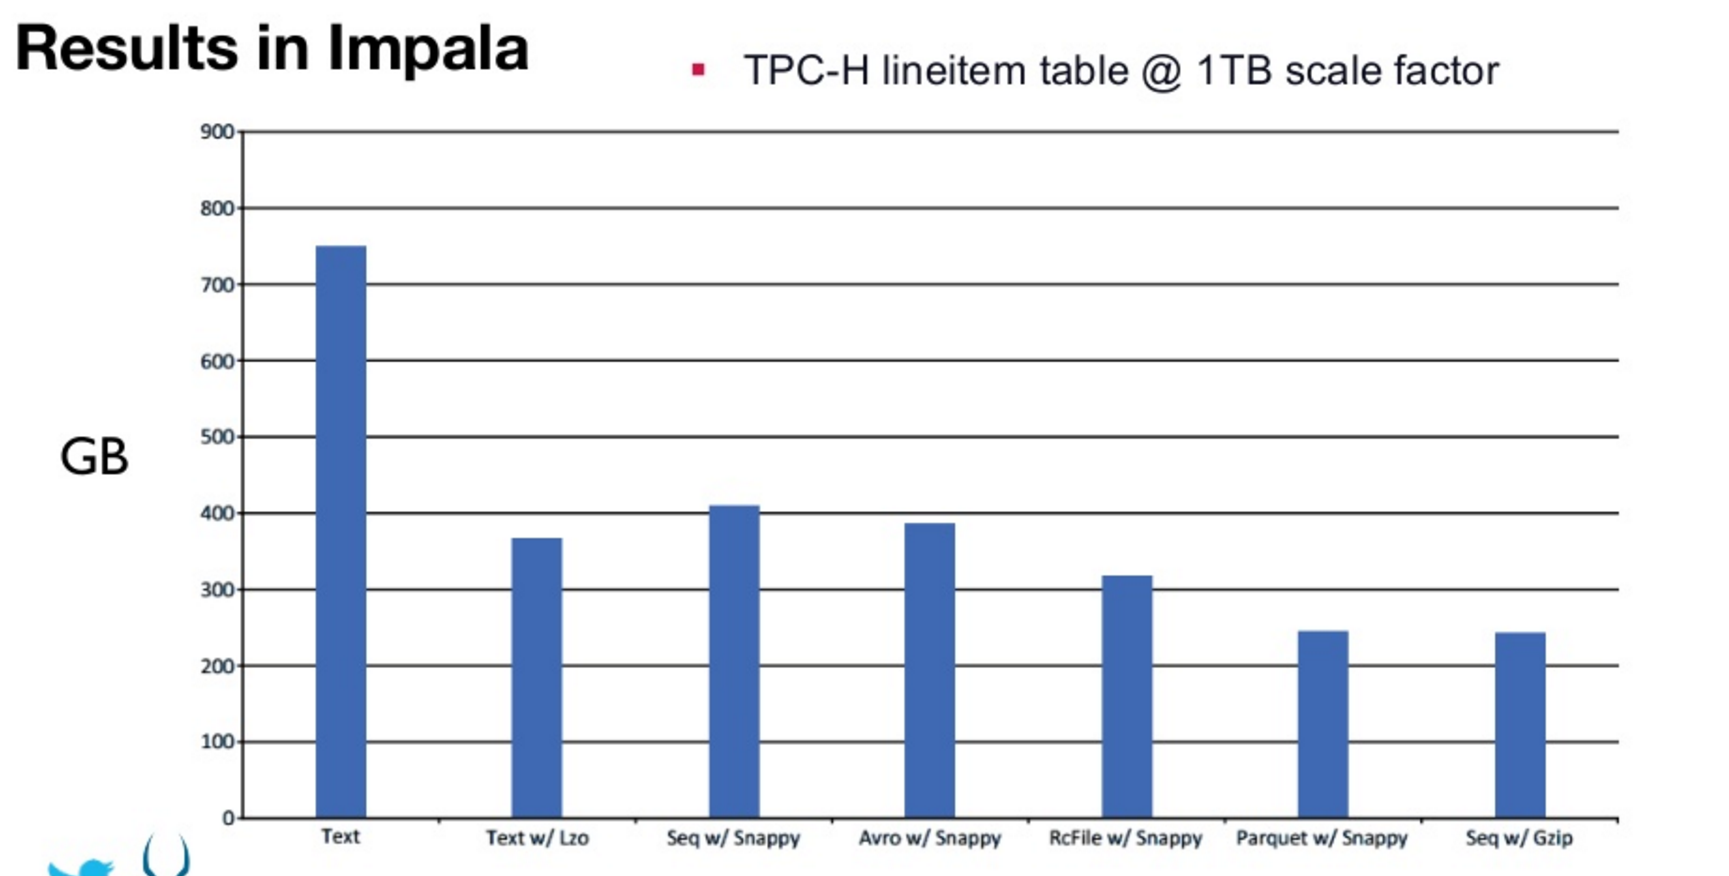
\includegraphics[scale=0.2]{graphics/parquetSpace}
\end{figure}

En este caso, para la compresión de los ficheros de \textit{Apache Parquet} utilizaremos la librería \textit{Snappy} \cite{snappyLib}, que es compatible con este formato. \textit{Snappy} es una librería de compresión y descompresión creada por Google cuya intención no es conseguir el mínimo tamaño de fichero, si no la mayor velocidad de compresión y descompresión.

%
% Marco regulador
%
\chapter{Marco Regulador \label{sec:MarcoRegulador}}

\section{Legislación aplicable}
Como se ha comentado anteriormente, la tecnología \textit{big data} permite el procesado de grandes cantidades de datos de forma más rápida que con tecnologías anteriores, con el propósito de obtener información valiosa de ella y generar conocimiento.

Este gran volumen de datos disponibles proviene de diferentes fuentes de información, que abarcan desde reportes anónimos hasta informes de uso de usuarios, donde estos están perfectamente identificados. Son este último tipo de datos los que pueden producir problemas legales, debido a la legislación vigente respecto a la privacidad de las personas.

La normativa nacional establece que ``un dato de carácter personal es cualquier información que permita identificarte o hacerte identificable'' y, por ello, ``reconoce al ciudadano la facultad de controlar sus datos personales y la capacidad para disponer y decidir sobre los mismos'' mediante el derecho fundamental a la protección de datos \cite{aepd}.

En España, es la \gls{AEPD} ``la autoridad de control independiente que vela por el cumplimiento de la normativa sobre protección de datos''. Además, ``garantiza y tutela el derecho fundamental a la protección de datos personales'' \cite{aepd}.

En la actualidad, es la Ley Orgánica 15/1999, de 13 de diciembre, de Protección de Datos de Carácter Personal \cite{leyPrivacidad} la que afecta al procesamiento de información que se realiza en los sistemas \textit{big data}. Esta, tiene que objetivo ``garantizar
y  proteger,  en  lo  que  concierne  al  tratamiento  de  los
datos personales, las libertades públicas y los derechos
fundamentales de las personas físicas, y especialmente
de su honor e intimidad personal y familiar'' \cite{leyPrivacidad}. Los derechos que incluye esta ley son \cite{derechosCiu}:

\clearpage
\begin{itemize}
\item Derecho de información: En el momento en que se procede a la recogida de los datos personales, el interesado debe ser informado previamente. 

\item Derecho de acceso: permite al ciudadano conocer y obtener gratuitamente información sobre sus datos de carácter personal que han sido tratados.

\item Derecho de rectificación: permite corregir errores, modificar los datos que resulten ser inexactos o incompletos y garantizar la certeza de la información tratada.

\item Derecho de cancelación: permite que se supriman los datos que resulten ser inadecuados o excesivos.

\item Derecho de oposición: permite al afectado que el tratamiento de sus datos de carácter personal no se realice o el cese de los mismo.
\end{itemize}

Con respecto a la Unión Europea, la ley que actualmente regula la protección y privacidad de los datos de carácter personal es el Reglamento (UE) 2016/679 del Parlamento Europeo y del Consejo de 27 de abril de 2016, relativo a la protección de las personas físicas en lo que respecta al tratamiento de datos personales y a la libre circulación de estos datos \cite{lawEU}.

Esta legislación europea ha sido reformada recientemente y se espera que para 2018 se aplique totalmente en todos los países de la zona euro. En esta reforma destacan, entre otras, la reforma al \Gls{derOlvido}, las grandes multas por el incumplimiento de las leyes de privacidad y el endurecimiento de los controles parentales \cite{rulesEU}. En general, esta reforma ha sido un endurecimiento de las medidas ya existentes para salvaguardar los derechos de los ciudadanos en esta nueva época digital.

Por tanto, con respecto al marco regulador que afecta a las aplicaciones del \textit{big data} se han de tener en cuenta aspectos como la seguridad, privacidad y correcta conservación de los datos personales de los usuarios, para proteger los derechos de los ciudadanos. De la misma forma, también debe asegurarse la transparencia de su uso frente a las autoridades.

\clearpage
\section{Estándares técnicos}
La utilización del \textit{Big Data} de forma masiva para el análisis de datos en el mundo empresarial, como ya se ha comentado, es una técnica relativamente reciente, por lo que no se ha producido un gran desarrollo con respecto a estándares de uso.

El primer estándar que se desarrolló data de noviembre de 2015, cuando la \gls{ITU}, agencia que depende de la \gls{ONU} y que es responsable de los problemas que conciernen a las tecnologías de información y comunicación, desarrolló y publicó el documento ITU-T Y.3600 (11/2015) \cite{estandar} titulado ``Big data - Cloud computing based requirements and capabilities''.

En este documento ``se presentan los requisitos, las capacidades y los casos de uso de los volúmenes masivos de datos (\textit{big data}) de computación en la nube, así como su contexto de sistema'' \cite{estandar}. Además, en este documento se establece la definición de \textit{big data} comentada en el apartado \ref{defBigData}.



%
% Diseño
%
\chapter{Análisis \label{sec:analisis}}
En este apartado se procederá a realizar un estudio de las funciones que deberá cumplir la arquitectura \textit{big data} implementada finalmente. Para ello, en este apartado se incluye la colección de requisitos del sistema definidos antes de comenzar el desarrollo del mismo.

Estos requisitos junto con el análisis de realizado de las tecnologías que se van a emplear, el estudio del problema propuesto por la organización del concurso y de los datos que se introducirán en el sistema, que serán las trazas de los viajes de los taxis de Nueva York, establecerán las guías para el diseño e implementación de la arquitectura \textit{big data} que se va a desarrollar y, tras la finalización de este proceso, serán utilizados para la comprobación de la verificación de completitud de los objetivos de este proyecto.

Al final de este apartado se incluirá una matriz de trazabilidad para trazar la relación entre los requisitos de usuario y los de software.

\section{Requisitos de usuario}
Para este proyecto, debido a la falta de un cliente, los requisitos de usuario han sido establecidos en conjunto por el autor y el tutor del trabajo. En estos se recogen las claves que deberá cumplir la arquitectura para lograr los objetivos establecidos y se dividen en dos conjuntos claramente diferenciados:

\begin{itemize}
\item \textbf{Requisitos de capacidad:} Que son aquellas funciones y objetivos que el sistema deberá cumplir para satisfacer al usuario.
\item \textbf{Requisitos de restricción:} Que establecen los límites que la arquitectura debe respetar a la hora de desarrollar el proyecto.
\end{itemize}

La nomenclatura que se utilizará para definir estos requisitos será la siguiente:

\begin{itemize}
\item \textbf{RU:} Que identificará al requisito como de usuario.
\item \textbf{C o R:} Que establecerá si el requisito es de capacidad (C) o de restricción (R).
\item \textbf{XX:} Donde XX es un número y que, con el conjunto de requisitos, formará una secuencia numérica que irá de 00 a 99. Este indica el número del requisito y la secuencia será independiente de cada tipo de requisito.
\end{itemize}

Por tanto, un requisito de usuario será identificado mediante la siguiente estructura RU-(C, R)-XX. La descripción de estos requisitos contará con los siguientes campos:


\begin{itemize}
\item \textbf{Identificador:} Identificación del requisito mediante la nomenclatura explicada anteriormente.
\item \textbf{Fuente:} Creador del requisito de usuario. Este podrá ser el autor o el tutor del proyecto.
\item \textbf{Necesidad:} Nivel de importancia respecto al cumplimiento del requisito:
\begin{itemize}
\item \textit{Fundamental:} Requisito de obligatorio cumplimiento en la implementación realizada.
\item \textit{Recomendable:} Requisito que es deseable que cumpla el sistema.
\item \textit{Prescindible:} Requisito que no supone ningún problema en caso de no ser implementado.
\end{itemize}
\item \textbf{Prioridad:} Establece la importancia del requisito respecto a la planificación de su implementación. Podrá ser \textit{alta}, \textit{media} o \textit{baja}.
\item \textbf{Descripción:} Texto que establecerá y describirá la función o restricción que deberá cumplir el sistema.
\end{itemize}

\begin{table}[htp!]
\centering
\caption{Requisito de usuario RU-C-01}
\label{ru1}
\begin{tabular}{|c|l|c|l|}
\hline
\textbf{IDENTIFICADOR} & \multicolumn{3}{l|}{RU-C-01}            \\ \hline
\textbf{FUENTE}        & \multicolumn{3}{l|}{Tutor}              \\ \hline
\textbf{NECESIDAD}     & Fundamental & \textbf{PRIORIDAD} & Alta \\ \hline
\multicolumn{4}{|c|}{\textbf{DESCRIPCIÓN}}                       \\ \hline
\multicolumn{4}{|l|}{\begin{tabular}[c]{@{}l@{}}Los ficheros a emplear por el sistema serán\\ las trazas de los viajes de taxis de la ciudad de Nueva York\\ proporcionados por la competición\end{tabular}} \\ \hline
\end{tabular}
\end{table}

\begin{table}[htp!]
\centering
\caption{Requisito de usuario RU-C-02}
\label{ru2}
\begin{tabular}{|c|l|c|l|}
\hline
\textbf{IDENTIFICADOR} & \multicolumn{3}{l|}{RU-C-02}            \\ \hline
\textbf{FUENTE}        & \multicolumn{3}{l|}{Tutor}              \\ \hline
\textbf{NECESIDAD}     & Fundamental & \textbf{PRIORIDAD} & Alta \\ \hline
\multicolumn{4}{|c|}{\textbf{DESCRIPCIÓN}}                       \\ \hline
\multicolumn{4}{|l|}{El sistema debe ser capaz de procesar los datos de forma masiva}\\ \hline
\end{tabular}
\end{table}

\begin{table}[htp!]
\centering
\caption{Requisito de usuario RU-C-03}
\label{ru3}
\begin{tabular}{|c|l|c|l|}
\hline
\textbf{IDENTIFICADOR} & \multicolumn{3}{l|}{RU-C-03}            \\ \hline
\textbf{FUENTE}        & \multicolumn{3}{l|}{Tutor}              \\ \hline
\textbf{NECESIDAD}     & Fundamental & \textbf{PRIORIDAD} & Alta \\ \hline
\multicolumn{4}{|c|}{\textbf{DESCRIPCIÓN}}                       \\ \hline
\multicolumn{4}{|l|}{\begin{tabular}[c]{@{}l@{}}El sistema debe de ser capaz de adaptar los datos al problema\\ y realizar la eliminación de los registros inválidos\end{tabular}} \\ \hline
\end{tabular}
\end{table}

\begin{table}[htp!]
\centering
\caption{Requisito de usuario RU-C-04}
\label{ru4}
\begin{tabular}{|c|l|c|l|}
\hline
\textbf{IDENTIFICADOR} & \multicolumn{3}{l|}{RU-C-04}            \\ \hline
\textbf{FUENTE}        & \multicolumn{3}{l|}{Tutor}              \\ \hline
\textbf{NECESIDAD}     & Fundamental & \textbf{PRIORIDAD} & Alta \\ \hline
\multicolumn{4}{|c|}{\textbf{DESCRIPCIÓN}}                       \\ \hline
\multicolumn{4}{|l|}{\begin{tabular}[c]{@{}l@{}}El sistema debe de ser capaz de analizar los datos\\ y responder a las consultas planteadas en el problema\end{tabular}} \\ \hline
\end{tabular}
\end{table}

\begin{table}[htp!]
\centering
\caption{Requisito de usuario RU-C-05}
\label{ru5}
\begin{tabular}{|c|l|c|l|}
\hline
\textbf{IDENTIFICADOR} & \multicolumn{3}{l|}{RU-C-05}            \\ \hline
\textbf{FUENTE}        & \multicolumn{3}{l|}{Tutor}              \\ \hline
\textbf{NECESIDAD}     & Fundamental & \textbf{PRIORIDAD} & Alta \\ \hline
\multicolumn{4}{|c|}{\textbf{DESCRIPCIÓN}}                       \\ \hline
\multicolumn{4}{|l|}{El sistema debe poder implementarse en diversos entornos y condiciones}\\ \hline
\end{tabular}
\end{table}

\begin{table}[htp!]
\centering
\caption{Requisito de usuario RU-C-06}
\label{ru6}
\begin{tabular}{|c|l|c|l|}
\hline
\textbf{IDENTIFICADOR} & \multicolumn{3}{l|}{RU-C-06}            \\ \hline
\textbf{FUENTE}        & \multicolumn{3}{l|}{Tutor}              \\ \hline
\textbf{NECESIDAD}     & Fundamental & \textbf{PRIORIDAD} & Media \\ \hline
\multicolumn{4}{|c|}{\textbf{DESCRIPCIÓN}}                       \\ \hline
\multicolumn{4}{|l|}{Se debe comparar el rendimiento de las diferentes configuraciones implementadas}\\ \hline
\end{tabular}
\end{table}

\begin{table}[htp!]
\centering
\caption{Requisito de usuario RU-C-07}
\label{ru7}
\begin{tabular}{|c|l|c|l|}
\hline
\textbf{IDENTIFICADOR} & \multicolumn{3}{l|}{RU-C-07}            \\ \hline
\textbf{FUENTE}        & \multicolumn{3}{l|}{Tutor}              \\ \hline
\textbf{NECESIDAD}     & Fundamental & \textbf{PRIORIDAD} & Media \\ \hline
\multicolumn{4}{|c|}{\textbf{DESCRIPCIÓN}}                       \\ \hline
\multicolumn{4}{|l|}{\begin{tabular}[c]{@{}l@{}}Se deben comparar el rendimiento del sistema con\\ diferentes tamaños del fichero de datos\end{tabular}} \\ \hline
\end{tabular}
\end{table}

\begin{table}[htp!]
\centering
\caption{Requisito de usuario RU-C-08}
\label{ru8}
\begin{tabular}{|c|l|c|l|}
\hline
\textbf{IDENTIFICADOR} & \multicolumn{3}{l|}{RU-C-08}            \\ \hline
\textbf{FUENTE}        & \multicolumn{3}{l|}{Autor del TFG}      \\ \hline
\textbf{NECESIDAD}     & Importante & \textbf{PRIORIDAD} & Normal\\ \hline
\multicolumn{4}{|c|}{\textbf{DESCRIPCIÓN}}                       \\ \hline
\multicolumn{4}{|l|}{\begin{tabular}[c]{@{}l@{}}No se define ninguna interfaz de usuario, el sistema\\  se ejecutará mediante la línea de comandos de Linux\end{tabular}} \\ \hline
\end{tabular}
\end{table}

\begin{table}[htp!]
\centering
\caption{Requisito de usuario RU-C-09}
\label{ru9}
\begin{tabular}{|c|l|c|l|}
\hline
\textbf{IDENTIFICADOR} & \multicolumn{3}{l|}{RU-C-09}            \\ \hline
\textbf{FUENTE}        & \multicolumn{3}{l|}{Autor del TFG}      \\ \hline
\textbf{NECESIDAD}     & Fundamental & \textbf{PRIORIDAD} & Alta \\ \hline
\multicolumn{4}{|c|}{\textbf{DESCRIPCIÓN}}                       \\ \hline
\multicolumn{4}{|l|}{\begin{tabular}[c]{@{}l@{}}Se debe documentar todo el estudio previo, el desarollo del\\ sistema y el análisis de los resultados obtenidos\end{tabular}} \\ \hline
\end{tabular}
\end{table}


\begin{table}[htp!]
\centering
\caption{Requisito de usuario RU-R-01}
\label{rur1}
\begin{tabular}{|c|l|c|l|}
\hline
\textbf{IDENTIFICADOR} & \multicolumn{3}{l|}{RU-R-01}            \\ \hline
\textbf{FUENTE}        & \multicolumn{3}{l|}{Tutor}              \\ \hline
\textbf{NECESIDAD}     & Fundamental & \textbf{PRIORIDAD} & Alta \\ \hline
\multicolumn{4}{|c|}{\textbf{DESCRIPCIÓN}}                       \\ \hline
\multicolumn{4}{|l|}{Se deberá usar \textit{Apache Spark} como librería principal de la arquitectura}\\ \hline
\end{tabular}
\end{table}

\begin{table}[htp!]
\centering
\caption{Requisito de usuario RU-R-02}
\label{rur2}
\begin{tabular}{|c|l|c|l|}
\hline
\textbf{IDENTIFICADOR} & \multicolumn{3}{l|}{RU-R-02}            \\ \hline
\textbf{FUENTE}        & \multicolumn{3}{l|}{Tutor}              \\ \hline
\textbf{NECESIDAD}     & Fundamental & \textbf{PRIORIDAD} & Alta \\ \hline
\multicolumn{4}{|c|}{\textbf{DESCRIPCIÓN}}                       \\ \hline
\multicolumn{4}{|l|}{Se deberá utilizar Python para realizar el desarrollo del sistema}\\ \hline
\end{tabular}
\end{table}

\section{Requisitos de software}
En este apartado, teniendo como base los requisitos de usuario enumerados anteriormente y con el conocimiento adquirido tras el análisis del problema planteado y del fichero de las trazas de los viajes de taxi, se definirán los requisitos de software. La nomenclatura utilizada para estos requisitos será ```RS-(F, NF-R, NF-D)-XX'' donde:

\begin{itemize}
\item \textbf{RS:} Que identificará al requisito como de usuario.
\item \textbf{F, NF-R o NF-D:} Que establecerá si el requisito es funcional (F) o no funcional, ya sea de restricción (R) o de documentación (D).
\item \textbf{XX:} Donde XX es un número y que, con el conjunto de requisitos, formará una secuencia numérica que irá de 00 a 99. Este indica el número del requisito y la secuencia será independiente de cada tipo de requisito.
\end{itemize}

Por tanto, un requisito de usuario será identificado mediante la siguiente estructura RU-(C, R)-XX. La descripción de estos requisitos contará con los siguientes campos:

\begin{itemize}
\item \textbf{RS:} Que identificará al requisito como de usuario.
\item \textbf{C o R:} Que establecerá si el requisito es de capacidad (C) o de restricción (R).
\item \textbf{XX:} Donde XX es un número y que, con el conjunto de requisitos, formará una secuencia numérica que irá de 00 a 99. Este indica el número del requisito y la secuencia será independiente de cada tipo de usuario.
\end{itemize}

\begin{itemize}
\item \textbf{Identificador:} Identificación del requisito mediante la nomenclatura explicada anteriormente.
\item \textbf{Fuente:} Que indica el requisito de usuario en el que se basa.
\item \textbf{Necesidad:} Se mantiene de la misma forma que en los requisitos de usuario.
\item \textbf{Prioridad:} Se mantiene de la misma forma que en los requisitos de usuario.
\item \textbf{Descripción:} Texto que establecerá y describirá el objetivo del requisito.
\end{itemize}

\begin{table}[htp!]
\centering
\caption{Requisito de software RS-F-01}
\label{rs1}
\begin{tabular}{|c|l|c|l|}
\hline
\textbf{IDENTIFICADOR}                                                                                       & \multicolumn{3}{l|}{RS-F-01}                                                                                                                                                                                                                                                                     \\ \hline
\textbf{FUENTE}                                                                                              & \multicolumn{3}{l|}{RU-C-01}                                                                                                                                                                                                                                                                     \\ \hline
\textbf{NECESIDAD}                                                                                           & Fundamental                                                                                       & PRIORIDAD                                                                                       & Alta                                                                                       \\ \hline
\multicolumn{4}{|c|}{\textbf{DESCRIPCIÓN}}                                                                                                                                                                                                                                                                                                                                                                      \\ \hline
\multicolumn{4}{|l|}{\begin{tabular}[c]{@{}l@{}}El fichero de datos que utilice el sistema será\\ el obtenido de la página del concurso \cite{grandChallenge},\\ que contendrá las trazas de los viajes de taxi de\\ la ciudad de Nueva York durante el año 2013, \\ siendo este fichero un \gls{CSV} de 33 GB.\\ Cada línea de este fichero representará un viaje y\\ cada registro contendrá 17 atributos\end{tabular}} \\ \hline
\end{tabular}
\end{table}

\begin{table}[htp!]
\centering
\caption{Requisito de software RS-F-02}
\label{rs2}
\begin{tabular}{|c|l|c|l|}
\hline
\textbf{IDENTIFICADOR}                                          & \multicolumn{3}{l|}{RS-F-02}                                                                                                                           \\ \hline
\textbf{FUENTE}                                                 & \multicolumn{3}{l|}{RU-C-02}                                                                                                                           \\ \hline
\textbf{NECESIDAD}                                              & Fundamental                                         & PRIORIDAD                                         & Alta                                         \\ \hline
\multicolumn{4}{|c|}{\textbf{DESCRIPCIÓN}}                                                                                                                                                                               \\ \hline
\multicolumn{4}{|l|}{\begin{tabular}[c]{@{}l@{}}El sistema debe ser capaz de procesar y realizar las \\ tareas que se ejecuten sobre los ficheros disponibles\\ sin problemas ni excepciones de ejecución.\end{tabular}} \\ \hline
\end{tabular}
\end{table}

\begin{table}[htp!]
\centering
\caption{Requisito de software RS-F-03}
\label{rs3}
\begin{tabular}{|c|l|c|l|}
\hline
\textbf{IDENTIFICADOR}                                   & \multicolumn{3}{l|}{RS-F-03}                                                                                                      \\ \hline
\textbf{FUENTE}                                          & \multicolumn{3}{l|}{RU-C-03}                                                                                                      \\ \hline
\textbf{NECESIDAD}                                       & Fundamental                                  & PRIORIDAD                                  & Alta                                  \\ \hline
\multicolumn{4}{|c|}{\textbf{DESCRIPCIÓN}}                                                                                                                                                   \\ \hline
\multicolumn{4}{|l|}{\begin{tabular}[c]{@{}l@{}}El sistema debe ser capaz de detectar los registros con errores y\\ de eliminarlos del fichero de datos para su posterior uso\end{tabular}} \\ \hline
\end{tabular}
\end{table}

\begin{table}[htp!]
\centering
\caption{Requisito de software RS-F-04}
\label{rs4}
\begin{tabular}{|c|l|c|l|}
\hline
\textbf{IDENTIFICADOR}                                          & \multicolumn{3}{l|}{RS-F-04}                                                                                                                              \\ \hline
\textbf{FUENTE}                                                 & \multicolumn{3}{l|}{RU-C-03}                                                                                                                              \\ \hline
\textbf{NECESIDAD}                                              & Fundamental                                          & PRIORIDAD                                          & Alta                                          \\ \hline
\multicolumn{4}{|c|}{\textbf{DESCRIPCIÓN}}                                                                                                                                                                                  \\ \hline
\multicolumn{4}{|l|}{\begin{tabular}[c]{@{}l@{}}El sistema debe ser capaz de transformar los atributos de  los\\ registros para adaptarlos a los requisitos del problema y guardarlos\\ para su posterior uso\end{tabular}} \\ \hline
\end{tabular}
\end{table}

\begin{table}[htp!]
\centering
\caption{Requisito de software RS-F-05}
\label{rs5}
\begin{tabular}{|c|l|c|l|}
\hline
\textbf{IDENTIFICADOR}                                 & \multicolumn{3}{l|}{RS-F-05}                                                                                                 \\ \hline
\textbf{FUENTE}                                        & \multicolumn{3}{l|}{RU-C-04}                                                                                                 \\ \hline
\textbf{NECESIDAD}                                     & Fundamental                                 & PRIORIDAD                                & Alta                                \\ \hline
\multicolumn{4}{|c|}{\textbf{DESCRIPCIÓN}}                                                                                                                                            \\ \hline
\multicolumn{4}{|l|}{\begin{tabular}[c]{@{}l@{}}El sistema debe ser capaz de analizar los datos procesados \\ anteriormente para calcular las diez rutas más frecuentes\end{tabular}} \\ \hline
\end{tabular}
\end{table}

\begin{table}[htp!]
\centering
\caption{Requisito de software RS-F-06}
\label{rs6}
\begin{tabular}{|c|l|c|l|}
\hline
\textbf{IDENTIFICADOR}                                       & \multicolumn{3}{l|}{RS-F-06}                                                                                                                     \\ \hline
\textbf{FUENTE}                                              & \multicolumn{3}{l|}{RU-C-04}                                                                                                                     \\ \hline
\textbf{NECESIDAD}                                           & Fundamental                                       & PRIORIDAD                                       & Alta                                       \\ \hline
\multicolumn{4}{|c|}{\textbf{DESCRIPCIÓN}}                                                                                                                                                                      \\ \hline
\multicolumn{4}{|l|}{\begin{tabular}[c]{@{}l@{}}El sistema debe ser capaz de analizar los datos procesados \\ anteriormente para calcular las diez zonas que más beneficios\\ reporten al taxista\end{tabular}} \\ \hline
\end{tabular}
\end{table}

\begin{table}[htp!]
\centering
\caption{Requisito de software RS-F-07}
\label{rs7}
\begin{tabular}{|c|l|c|l|}
\hline
\textbf{IDENTIFICADOR}                            & \multicolumn{3}{l|}{RS-F-07}                                                                                 \\ \hline
\textbf{FUENTE}                                   & \multicolumn{3}{l|}{RU-C-05}                                                                                 \\ \hline
\textbf{NECESIDAD}                                & Fundamental                           & PRIORIDAD                           & Alta                           \\ \hline
\multicolumn{4}{|c|}{\textbf{DESCRIPCIÓN}}                                                                                                                       \\ \hline
\multicolumn{4}{|l|}{\begin{tabular}[c]{@{}l@{}}El sistema debe ser implementado en el entorno doméstico\\ tanto en el modo local como distribuido\end{tabular}} \\ \hline
\end{tabular}
\end{table}

\begin{table}[htp!]
\centering
\caption{Requisito de software RS-F-08}
\label{rs8}
\begin{tabular}{|c|l|c|l|}
\hline
\textbf{IDENTIFICADOR}                             & \multicolumn{3}{l|}{RS-F-07}                                                                                    \\ \hline
\textbf{FUENTE}                                    & \multicolumn{3}{l|}{RU-C-05}                                                                                    \\ \hline
\textbf{NECESIDAD}                                 & Fundamental                            & PRIORIDAD                            & Alta                            \\ \hline
\multicolumn{4}{|c|}{\textbf{DESCRIPCIÓN}}                                                                                                                           \\ \hline
\multicolumn{4}{|l|}{\begin{tabular}[c]{@{}l@{}}El sistema debe ser implementado en el entorno universitario\\ tanto en el modo local como distribuido\end{tabular}} \\ \hline
\end{tabular}
\end{table}

\begin{table}[htp!]
\centering
\caption{Requisito de software RS-F-09}
\label{rs9}
\begin{tabular}{|c|l|c|l|}
\hline
\textbf{IDENTIFICADOR}                                           & \multicolumn{3}{l|}{RS-F-09}                                                                                                                               \\ \hline
\textbf{FUENTE}                                                  & \multicolumn{3}{l|}{RU-C-06}                                                                                                                               \\ \hline
\textbf{NECESIDAD}                                               & Fundamental                                           & PRIORIDAD                                          & Media                                          \\ \hline
\multicolumn{4}{|c|}{\textbf{DESCRIPCIÓN}}                                                                                                                                                                                    \\ \hline
\multicolumn{4}{|l|}{\begin{tabular}[c]{@{}l@{}}Se compararán los resultados de rendimiento de los diferentes\\ modos implementados, local o distribuido, y los diferentes \\ entornos, doméstico y universitario\end{tabular}} \\ \hline
\end{tabular}
\end{table}

\begin{table}[htp!]
\centering
\caption{Requisito de software RS-F-10}
\label{rs10}
\begin{tabular}{|c|l|c|l|}
\hline
\textbf{IDENTIFICADOR}                                      & \multicolumn{3}{l|}{RS-F-10}                                                                                                                   \\ \hline
\textbf{FUENTE}                                             & \multicolumn{3}{l|}{RU-C-07}                                                                                                                   \\ \hline
\textbf{NECESIDAD}                                          & Fundamental                                      & PRIORIDAD                                      & Media                                      \\ \hline
\multicolumn{4}{|c|}{\textbf{DESCRIPCIÓN}}                                                                                                                                                                   \\ \hline
\multicolumn{4}{|l|}{\begin{tabular}[c]{@{}l@{}}Se realizarán diversos ficheros de datos a partir del\\ original, de menor tamaño, para comparar los resultados\\ de procesamiento entre ellos\end{tabular}} \\ \hline
\end{tabular}
\end{table}

\begin{table}[htp!]
\centering
\caption{Requisito de software RS-F-011}
\label{rs11}
\begin{tabular}{|c|l|c|l|}
\hline
\textbf{IDENTIFICADOR}                                              & \multicolumn{3}{l|}{RS-F-11}                                                                                                                                        \\ \hline
\textbf{FUENTE}                                                     & \multicolumn{3}{l|}{RU-C-08}                                                                                                                                        \\ \hline
\textbf{NECESIDAD}                                                  & Fundamental                                             & PRIORIDAD                                             & Media                                             \\ \hline
\multicolumn{4}{|c|}{\textbf{DESCRIPCIÓN}}                                                                                                                                                                                                \\ \hline
\multicolumn{4}{|l|}{\begin{tabular}[c]{@{}l@{}}La ejecución de las diferentes funciones del sistema\\ se realizará a través de la de línea de comandos de Linux,\\ mediante la introducción de la función y sus argumentos\end{tabular}} \\ \hline
\end{tabular}
\end{table}

\begin{table}[htp!]
\centering
\caption{Requisito de software RS-NF-D-01}
\label{rsnf1}
\begin{tabular}{|c|l|c|l|}
\hline
\textbf{IDENTIFICADOR}                                                                                & \multicolumn{3}{l|}{RS-NF-D-01}                                                                                                                                                                                                                                              \\ \hline
\textbf{FUENTE}                                                                                       & \multicolumn{3}{l|}{RU-C-09}                                                                                                                                                                                                                                                 \\ \hline
\textbf{NECESIDAD}                                                                                    & Fundamental                                                                                 & PRIORIDAD                                                                                & Alta                                                                                \\ \hline
\multicolumn{4}{|c|}{\textbf{DESCRIPCIÓN}}                                                                                                                                                                                                                                                                                                                                           \\ \hline
\multicolumn{4}{|l|}{\begin{tabular}[c]{@{}l@{}}Se realizará una memoria del trabajo realizado, donde\\ se incluirá el estado del arte y el análisis de la situación\\ de las tecnologías utilizadas, así como, un análisis de los\\ pasos seguidos durante el desarrollo de la arquitectura, \\ incluyendo el diseño, la implementación y los resultados\\ obtenidos.\end{tabular}} \\ \hline
\end{tabular}
\end{table}

\begin{table}[htp!]
\centering
\caption{Requisito de software RS-NF-R-01}
\label{rsfn2}
\begin{tabular}{|c|l|c|l|}
\hline
\textbf{IDENTIFICADOR}                                                   & \multicolumn{3}{l|}{RS-NF-R-01}                                                                                                                                                       \\ \hline
\textbf{FUENTE}                                                          & \multicolumn{3}{l|}{RU-R-01}                                                                                                                                                          \\ \hline
\textbf{NECESIDAD}                                                       & Fundamental                                                    & PRIORIDAD                                                   & Alta                                                   \\ \hline
\multicolumn{4}{|c|}{\textbf{DESCRIPCIÓN}}                                                                                                                                                                                                                       \\ \hline
\multicolumn{4}{|l|}{\begin{tabular}[c]{@{}l@{}}Se utilizará \textit{Apache Spark} como librería principal del \\ proyecto, siendo utilizada para gestionar los procesos\\ llevados a cabo por el sistema, tanto en el modo local\\ como en el distribuido.\end{tabular}} \\ \hline
\end{tabular}
\end{table}

\begin{table}[htp!]
\centering
\caption{Requisito de software RS-NF-R-02}
\label{rsnf3}
\begin{tabular}{|c|l|c|l|}
\hline
\textbf{IDENTIFICADOR}                                      & \multicolumn{3}{l|}{RS-NF-R-02}                                                                                                              \\ \hline
\textbf{FUENTE}                                             & \multicolumn{3}{l|}{RU-R-02}                                                                                                                 \\ \hline
\textbf{NECESIDAD}                                          & Fundamental                                       & PRIORIDAD                                     & Alta                                     \\ \hline
\multicolumn{4}{|c|}{\textbf{DESCRIPCIÓN}}                                                                                                                                                                 \\ \hline
\multicolumn{4}{|l|}{\begin{tabular}[c]{@{}l@{}}Se utilizará Python como lenguaje de programación para\\ el desarrollo del sistema, utilizando la API de \textit{Apache Spark},\\ pyspark, para ello.\end{tabular}} \\ \hline
\end{tabular}
\end{table}

\section{Matriz de trazabilidad}
\begin{figure}[htp!]
\centering
\caption{Matriz de trazabilidad de los requisitos}
\label{tab:matrizReq}
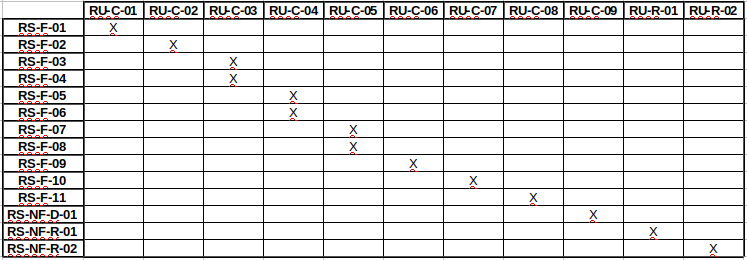
\includegraphics[scale=0.6]{graphics/matriz}
\end{figure}

%
% Diseño
%
\chapter{Diseño \label{sec:disenho}}

\section{Introducción}
Tras el análisis del panorama y las tecnologías \textit{big data} y, en especial, de las que van a ser utilizadas en este proyecto, en este apartado, se procederá con la explicación del diseño de la arquitectura \textit{big data} que, posteriormente, se implementará presentando diferentes configuraciones y alternativas.

En cuanto a la estructura de este apartado, en primer lugar procederemos a presentar una visión general del sistema y se establecerán las unidades o bloques de funcionamiento. Posteriormente, se tratará la arquitectura del sistema, teniendo en cuenta los diferentes entornos en los que seá implementado y, finalmente, se detallarán los componentes que conformarán las diferentes unidades funcionales del sistema y la interacción entre ellos para el funcionamiento del sistema.

\section{Visión general y unidades funcionales \label{unitFunc}}
Como se ha comentado en la introducción, el objetivo del proyecto es diseñar implementar una arquitectura \textit{big data} para procesar las trazas de los recorridos de taxis de la ciudad de Nueva York. Debido a la naturaleza del mismo, dónde se busca analizar diferentes configuraciones y detectar sus limitaciones, la implementación de este sistema se llevará a cabo en dos entornos diferenciados primero uno doméstico y, posteriormente, uno más realista, en la universidad.

\clearpage
Esta implementación en dos entornos hará que el diseño varíe ligeramente para cada uno de ellos, adaptándose a las condiciones técnicas que presentan. Estas diferencias solo afectarán al almacenamiento de datos por lo que la base principal de la arquitectura será la misma.

Con respecto al diseño del sistema y, también debido por el carácter experimental del proyecto se ha establecido un único rol de usuario en el sistema qué será el de administrador. Esta decisión ha sido tomada ya que no se pretende implementar el sistema para su uso en producción y, por tanto, no se ve necesaria una distinción entre tipos de usuario. Es decir, el sistema solo va a ser utilizado por un único usuario que hará todas las pruebas de rendimiento y por ello no se plantea establecer limitaciones en las funciones del sistema para otros posibles usos ni introducir nuevos roles.

En este sistema, por tanto, el administrador tendrá la capacidad de realizar los procesos de carga de datos, procesamiento de los mismos y ejecución de las consultas y obtención de resultados. Está funciones comentadas son las que darán lugar a las tres unidades funcionales del sistema (figura \ref{fig:esquemagen}), que serán las siguientes y tendrán la función descrita:

\begin{figure}[htp!]
\centering
\caption{Esquema general del sistema incluyendo las unidades funcionales}
\label{fig:esquemagen}
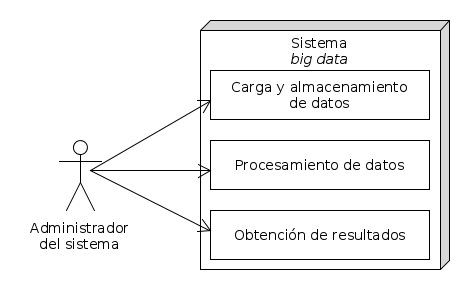
\includegraphics[scale=0.7]{diagramas/esquemaGen}
\end{figure}

\begin{itemize}
\item \textbf{Carga y almacenamiento de datos:} La carga de los datos es la primera tarea que ejecutará el usuario para que el sistema cuente con las trazas a procesar y que estas puedan ser distribuidas por los nodos. En este proyecto estos datos se corresponden con los viajes de los taxis realizados en la ciudad de Nueva York durante el año 2013 y son aportados por la organización del concurso.

En general, en los sistemas \textit{big data} el conjunto de datos proviene de diferentes fuentes, haciendo que estos tengan que ser procesados para lograr una estructura homogénea de los mismos. Sin embargo, en esta ocasión no se da el caso, donde solo se tiene un fichero \gls{CSV} con todas las trazas del año y que tienen la misma estructura.

Esta unidad, también será la encargada de almacenar los ficheros de datos cargados inicialmente por el usuario, así como, aquellos que genere el sistema. Es decir, también almacenará los ficheros procesados por el sistema y los resultados de las consultas ejecutadas.

\item \textbf{Procesado de datos:} Los datos originales tienen que ser procesados para ajustarse a los requisitos del desafío siendo, para ello, transformados y limpiados. Es decir, esta unidad, por un lado, transformará ciertos atributos de las trazas para crear nuevos a partir de los primeros, para facilitar cálculos y cumplir las normas del concurso. Por otro lado, realizará una limpieza de trazas inválidas, donde falte información o este corrupta y, también, de atributos innecesarios para los cálculos que se realizarán y, de esta forma, ahorrar espacio.

\item \textbf{Ejecución de las consultas y obtención de resultados:} Este bloque funcional es el encargado de obtener los resultados a partir del análisis de los datos contenidos en el sistema. Debido a la existencia de dos consultas, el usuario ejecutará en el sistema la consulta o consultas deseadas y este devolverá los datos de esta o estas en forma de archivo de texto plano con el nombre establecido por el usuario, que será situado en la carpeta de resultados del sistema.
\end{itemize}

\section{Arquitectura del sistema}
Gracias a las posibilidades que ofrece \textit{Apache Spark}, se ha diseñado la arquitectura ofreciendo dos posibles modos de ejecución con el fin de crear un sistema que se pueda adaptar a las diferentes situaciones que se puedan dar en cuanto a escalabilidad y disponibilidad. Esto nos permitirá además, ver las diferencias de rendimiento entre las diferentes configuraciones de forma más clara para las distintas situaciones y pruebas.

\begin{figure}[htp!]
\centering
\caption{Modos de ejecución del sistema \textit{bigdata}}
\label{fig:modoEjecución}
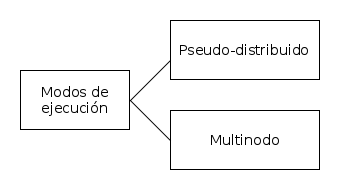
\includegraphics[scale=0.6]{diagramas/modoExec}
\end{figure}

Los dos modos de ejecución disponibles serán el pseudo-distribuido, donde solo se cuenta con un dispositivo que será maestro y esclavo a la vez y, el multinodo, donde se contarán con varios nodos, donde habrá un maestro y varios esclavos. Además, en el caso de la configuración multinodo se establecerán distintas distribuciones nodos y formas de transmisión de datos entre ellos.

\subsection{Modo pseudo-distribuido \label{disStandalone}}
En este modo de ejecución se dispone únicamente de un solo nodo, es decir, de una sola máquina que hará las veces de maestro y esclavo, pudiendo así establecerse un sistema completo. 

En este, se creara un objeto \textit{SparkContext} que será el maestro y que asignará los trabajos de procesamiento a diferentes procesos que se ejecutarán en paralelo en los diferentes núcleos del sistema, que harán de esclavos.

Este tipo de configuración tiene sus ventajas, siendo la principal la velocidad y sencillez con la que se desplegar el sistema en un ordenador, siendo únicamente necesario crear el objeto, como en la figura \ref{cod:instanciaSpark}, para contar con una instancia de este sistema lista para operar. Otras de las ventajas es la sencillez de mantenimiento del sistema, ya que al tratarse de una única máquina, no hay errores de conexión entre nodos, ni pérdidas de datos. 

\begin{lstlisting}[label=cod:instanciaSpark,language=Python,frame=single,caption=Modo pseudo-distribuido: Creación instancia de Spark]
CONF = SparkConf()
CONF.setAppName(APP_NAME)
CONF.setMaster("local[*]")
SPARK = SparkSession.builder.config(conf=CONF).getOrCreate()
\end{lstlisting}

Por otro lado, si comparamos la capacidad de procesamiento de este modo de ejecución con el de un clúster de varios nodos, es evidente que la capacidad del modo pseudo-distribuido será muy inferior en los casos en el que los archivos de datos sean muy grandes, siendo este la única y principal desventaja de este modo de ejecución. Esta inferioridad será demostrada en el apartado \ref{sec:resultados}.

\subsection{Modo distribuido o multinodo \label{disMultinodo}}
En este modo de ejecución se cuenta con más de una máquina para ser utilizada por el sistema, siendo la configuración utilizada en la gran mayoría arquitecturas \textit{big data} que se utilizan. 

En este tipo de ejecución se cuenta con una máquina que hará de maestro y distribuirá las tareas sobre el resto de nodos, los esclavos, y ella misma, para lograr la máxima eficacia de procesamiento. Es decir, el maestro creará un objeto \textit{SparkContext} que será el que distribuya los trabajos a los nodos conectados y recogera los resultados, como se muestra en la figura \ref{fig:clusterSpark} \cite{clusterfoto}.

\begin{figure}[htp!]
\centering
\caption{Modo distribuido o multinodo de \textit{Spark} \cite{clusterfoto}}
\label{fig:clusterSpark}
\includegraphics[scale=0.6]{graphics/sparkCluster}
\end{figure}

En este caso, la ventaja de esta configuración es la gran capacidad de procesamiento que se puede obtener, especialmente si las tareas ha realizar requieren gran cantidad de potencia de procesamiento, al disponer de la suma de los procesadores y de la memoria \gls{RAM} de los nodos del sistema.

La principal desventaja de este, que es su principal punto débil, se encuentra en la conexión entre los nodos, cuya calidad y velocidad afectará al rendimiento del sistema de forma muy importante. Es decir, el problema en los sistemas distribuidos proviene de la conexión de red entre los equipos, donde se pueden producir cuellos de botella en el envío de datos entre ellos. Estos pueden hacer que aunque la potencia teórica del sistema sea muy alta se obtengan malos rendimientos de procesamiento que hagan que el sistema no resulte rentable.

Otro de las desventajas de esta configuración es el coste de mantenimiento del conjunto de las máquinas y los dispositivos necesarios para mantener el clúster en funcionamiento.

Debido a que la implementación del sistema se realizará en dos entornos diferentes, con características diferentes en cuanto a la conexión de los equipos, se diseñaran dos configuraciones del sistema, una para el clúster doméstico y otra para el universitario.

\subsubsection{Clúster doméstico \label{disDomestico}}
Esta implementación de \textit{Apache Spark} tiene como objetivo comprobar la eficiencia y capacidad de procesamiento de un sistema \textit{big data} donde la limitación está en las máquinas. Para ello se contará con tres máquinas de modestas prestaciones que formarán un clúster que será comparado con la configuración pseudo-distribuida del entorno doméstico.

El número de máquinas que formarán este clúster serán tres, un portátil que hará de maestro y dos esclavos, un portátil y un sobremesa, como se puede observar en la figura \ref{fig:clusterDomestico}. Todos estos nodos estarán conectados a la red mediante cables Ethernet RJ45 Cat.5e UTP y contarán con Ubuntu 16.10 \cite{ubuntu} como versión del sistema operativo.

\begin{figure}[htp!]
\centering
\caption{Arquitectura del clúster doméstico}
\label{fig:clusterDomestico}
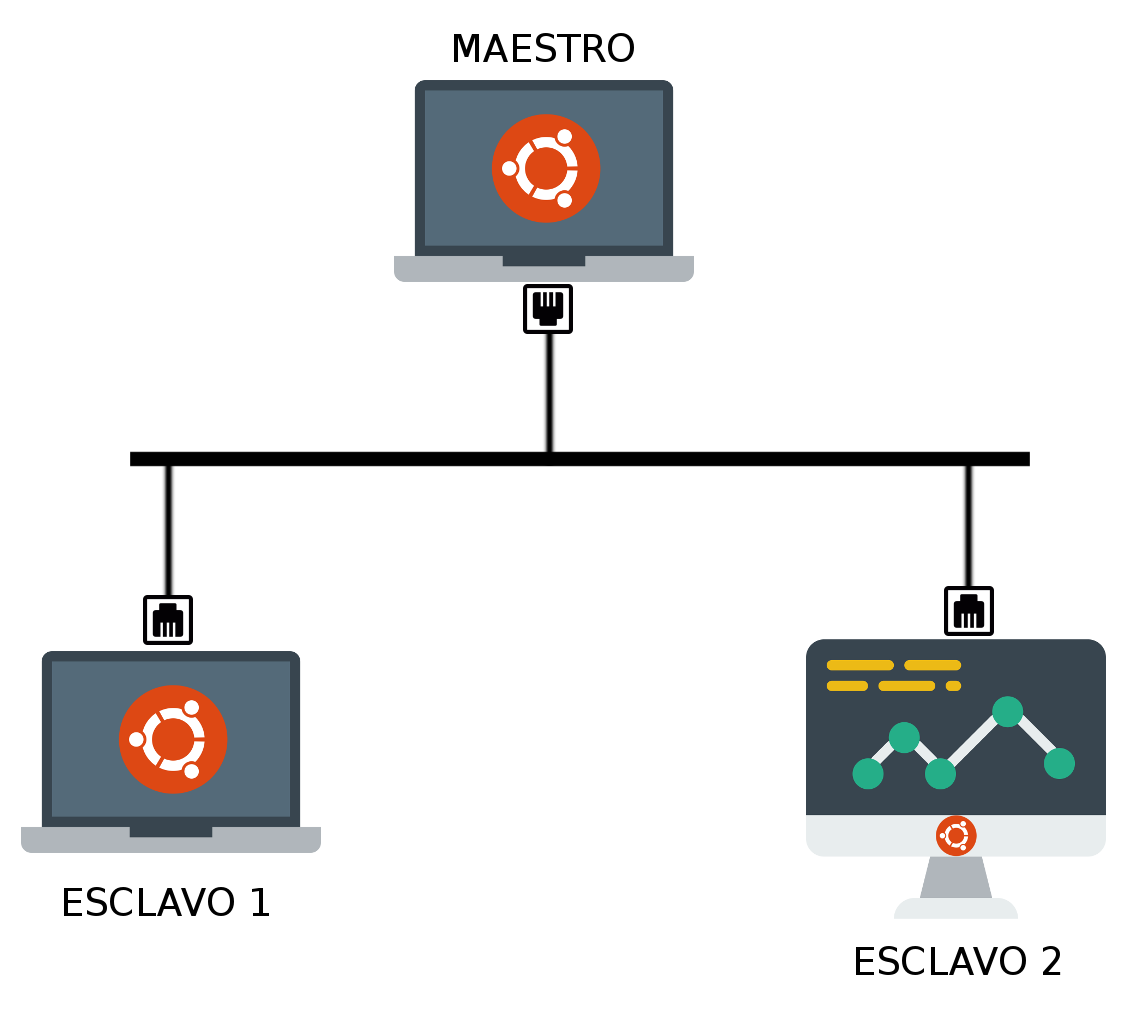
\includegraphics[scale=0.3]{graphics/clusterDomestico}
\end{figure}

Uno de los aspectos claves y diferenciadores con respecto al clúster universitario, es que en este no se cuenta con un \gls{NFS} por lo que para que todos los nodos del sistema cuenten con los datos se decide establecer un mecanismo de replicación de estos.

\textit{Apache hadoop} es la tecnología utilizada para montar este mecanismo de replicación mediante el uso de su sistema distribuido de ficheros (\gls{HDFS}) que resulta óptimo para esta configuración. Este mecanismo nos permitirá tener los datos en cada nodo del clúster y, así, lo único que circulará por la red serán las tareas que el maestro asigne a los esclavos y los resultados que estos obtengan tras su procesamiento. 

Esto evitará el tráfico que generaría transmitir los datos a procesar con la tarea asignada a los nodos esclavos, mejorando el rendimiento de la arquitectura.

\begin{figure}[htp!]
\centering
\caption{Esquema del sistema de replicación \gls{HDFS}}
\label{fig:hdfs}
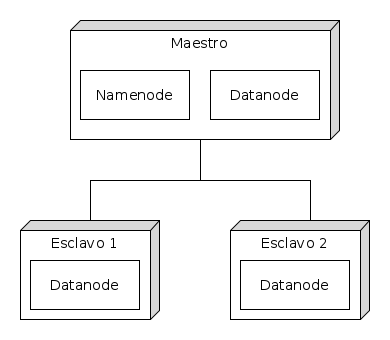
\includegraphics[scale=0.6]{diagramas/hadoop}
\end{figure}

Como se aprecia en la figura \ref{fig:hdfs} que muestra el esquema del sistema de replicación, para su funcionamiento, en cada nodo se necesita un proceso \textit{datanode} ejecutándose, que será el que se encargue de el almacenamiento de los datos en la máquina. Además, para controlar el estado de los \textit{datanodes} se necesita un proceso \textit{namenode}, que se ejecutará en el nodo maestro.

Debido a la buena interoperatividad de \textit{Apache Spark} con este sistema de replicación de datos, la implementación de este no implicará mayores cambios que la indicación de las rutas de los archivos a la que este sistema le asigne a los archivos manteniendo así la estructura de las unidades de procesamiento de los datos y las consultas.

Este diseño, tiene sus ventajas y desventajas con respecto a las demás configuraciones, pseudo-distribuida y multinodo universitario. En cuanto a las ventajas, la capacidad de procesamiento será mayor que la de el modo pseudo-distribuido al contar con un mayor número de núcleos y \gls{RAM}, aunque será menor que con respecto a la del clúster universitario al contar con menos nodos.

Otra de sus ventajas es la sencillez y el bajo coste que supone montar el sistema de replicación, en comparación con el \gls{NFS} del clúster universitario. Aunque tiene la desventaja del desaprovechamiento de espacio de disco en los nodos, donde cada uno tiene una copia de los datos aunque no los utilicen totalmente. Además, otra desventaja se produce al realizar el proceso de replicación, que debido a las limitaciones de la red, se realiza de forma lenta, necesitando un largo periodo de tiempo.

Finalmente, se puede comentar como desventaja que el nivel de configuraciones a realizar para montar este sistema es mayor que cualquiera de los otros que se implementarán debido a que, a parte de configurar \textit{Apache Spark}, habrá que configurar \textit{Apache Hadoop}.

\subsubsection{Clúster universitario \label{disUni}}
Como se ha indicado anteriormente, este clúster es el que representa un sistema \textit{big data} más realista, ya que, sus nodos tienen todos las mismas características y se dispone de un sistema de archivos en red que hace que el acceso a los datos sea más sencillo y eficiente. Además, la conexión entre los nodos se realiza a través de fibra óptica, obteniendo una velocidad superior al cable de red utilizado en el clúster doméstico.

Debido a la existencia de este sistema \gls{NFS} todos los nodos tienen acceso a los mismos datos que el nodo maestro, con la misma ruta de acceso, cosa que simplifica en gran manera la gestión de archivos. Además este sistema hace que no sea necesario un sistema de replicación, por lo que el proceso de  configuración del sistema es poco más complicado que el de la configuración pseudo-distribuida, diferenciándose únicamente en el procedimiento para conectar los nodos que formarán parte del clúster.

\begin{figure}[ht]
\centering
\caption{Arquitectura del clúster universitario}
\label{fig:clusterUni}
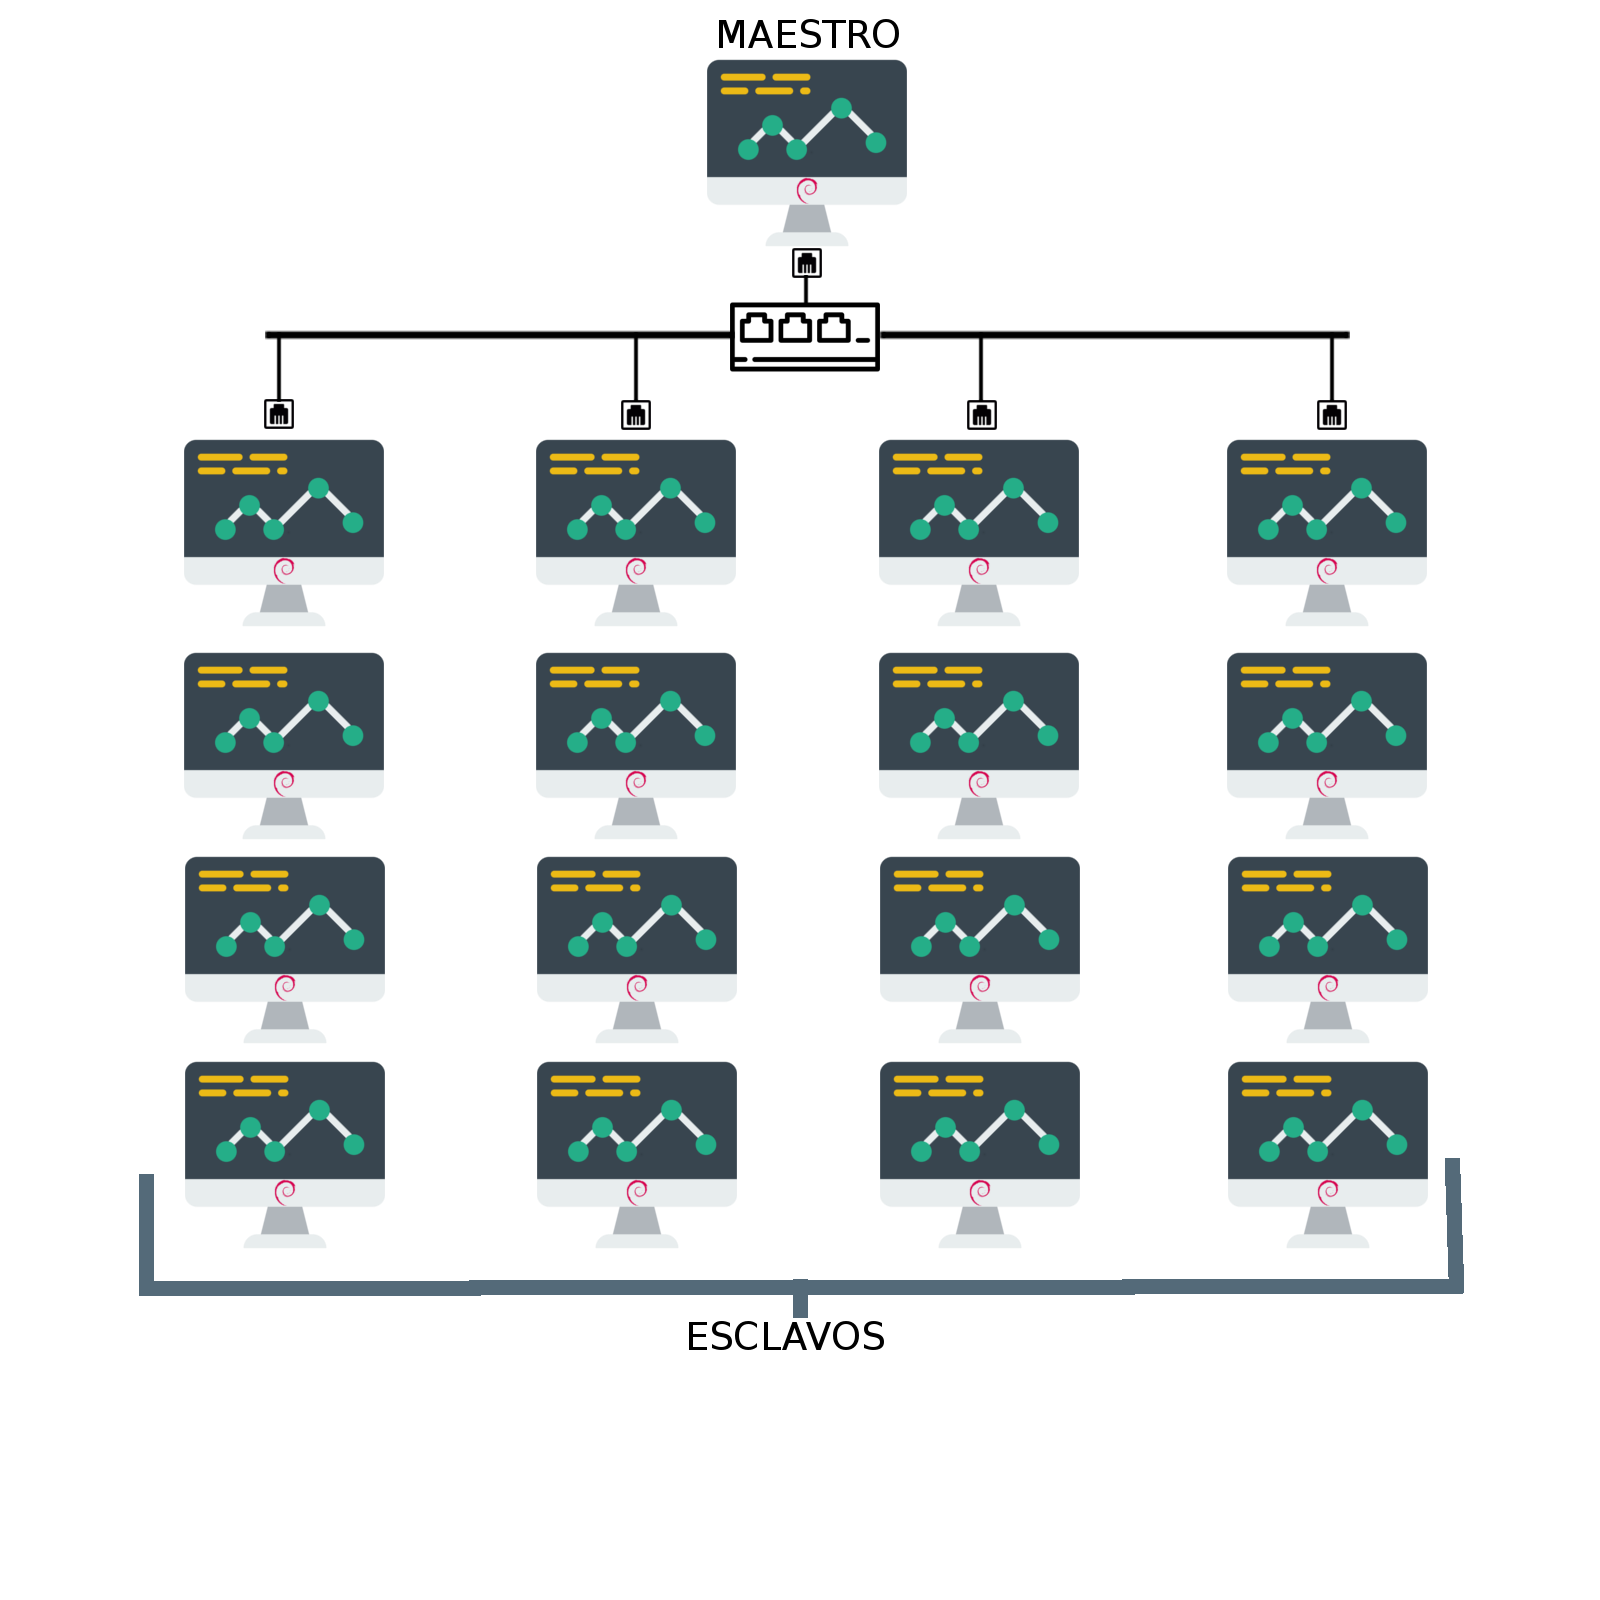
\includegraphics[scale=0.25]{graphics/clusterUni}
\end{figure}

En la figura \ref{fig:clusterUni} se puede apreciar la arquitectura de este clúster, este contará con un nodo que hará de maestro y que contendrá el objeto \textit{SparkContext} que será el encargado de distribuir las tareas entre todos los nodos y de recibir los resultados de estos y juntarlos para obtener los finales. El resto de nodos, que variarán en número para las diferentes pruebas, harán de esclavos. 

Este diseño, como todos los demás, tiene sus ventajas y desventajas. La principal ventaja es la capacidad de procesamiento que puede alcanzar, al contar con un alto número de nodos el número de \gls{CPU}s y gran cantidad de memoria \gls{RAM}, la capacidad de cálculo de esta configuración es elevada. Además, el sistema \gls{NFS} con conexiones de fibra óptica, hace que la velocidad de conexión sea elevada, permitiendo aprovechar la potencia de la arquitectura.

Por otro lado, este mismo sistema de ficheros hace que la configuración del sistema sea sencilla, ya que, no es necesario montar un mecanismo de replicación. Sin embargo, este también produce desventajas en el sistema, por un lado, tenemos una limitación en la cuota de disco a utilizar por el usuario, limitada a 30GB. Por otro lado, el coste de mantener este sistema es el más alto, debido al gran número de máquinas utilizadas para montarlo, así como para mantener el sistema de ficheros en red.

\section{Descripción de las unidades funcionales y sus componentes}
El sistema \textit{big data} estará compuesto por diferentes módulos que se relacionarán entre sí para el correcto funcionamiento del mismo, es decir, para que el flujo de las actividades y procesos a ejecutar sea continuo.

Como se ha comentado anteriormente, la implementación del sistema se realizará sobre dos entornos diferentes, uno doméstico, donde se contara con el sistema de replicación \gls{HDFS} y, otro universitario, donde se cuenta con un sistema \gls{NFS}. Esto hará que se presenten dos diseños para el almacenamiento de los datos, que aunque en su estructuración sean muy similares, tengan sus diferencias.

Por ello, como se indicó en el apartado \ref{unitFunc}, el sistema contará con tres unidades funcionales, dos de las cuales serán iguales para todas las configuraciones del sistema, la encargada del tratamiento de los datos y la obtención de resultados, y, una, la encargada de la carga y almacenamiento de los datos, que dependerá del sistema de ficheros usado.

En este apartado, por tanto, se describirá el diseño de las diferentes unidades funcionales del sistema, analizando los componentes que las forman y, tras ello, se tratarán las interacciones entre ellas y el usuario.

\subsection{Carga y almacenamiento de datos \label{diseñoFich}}
Esta unidad funcional será la única de la arquitectura que varíe dependiendo de la configuración que se utilice. Aunque la abstracción general será igual para los dos diseños, es decir, la estructura del sistema de ficheros será la misma, el diseño global no será el mismo por la diferencia en las características y funcionamiento de estos sistemas. 

Por tanto, diferenciaremos dos diseños, el primero que utilizará las herramientas ya disponibles en el sistema que será utilizado por el modo pseudo-distribuido, en ambos entornos, y por el modo distribuido en el entorno universitario, que al tratarse de un sistema \gls{NFS} funciona de la misma forma que el anterior. El segundo diseño será utilizado por el modo distribuido del clúster doméstico, que necesita del sistema de replicación \gls{HDFS} para su funcionamiento y que cambia el proceso de carga de datos y la estructura de almacenamiento.

El objetivo de este bloque funcional es alojar los datos a los que recurrirá el sistema para realizar el resto de tareas, ya sea el tratamiento de los mismos o el análisis para obtener los resultados a las consultas. Por tanto, al diferenciarse dos tipos de datos, unos, cargados por el usuario y sin procesar y, otros, ya tratados por el sistema, el diseño deberá contemplar una separación entre ellos. Además, el usuario también tendrá que ser capaz de acceder a los ficheros de los resultados, que también serán almacenados en el sistema.

\begin{figure}[htp!]
\centering
\caption{Estructura general para el almacenado de datos}
\label{fig:estructAlmacen}
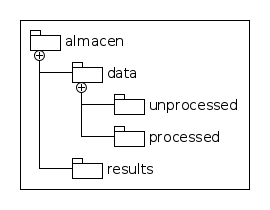
\includegraphics[scale=0.8]{diagramas/estrucAlmacen}
\end{figure}

Por tanto, la estructura del sistema de ficheros, independientemente de la implementación, tendrá una organización como se puede observar en la figura \ref{fig:estructAlmacen}, donde cada tipo de dato que maneje el sistema tendrá un apartado específico.

Por un lado, se diferenciará entre los datos con los que trabajará el sistema, es decir, las trazas de los taxis, que serán almacenadas en la carpeta ``data'' y, dentro de esta, se distinguirá también entre los ficheros cargados por el usuario, que irán destinados a la carpeta ``unprocessed'' y los tratados por el sistema, que se almacenarán en la carpeta ``processed'', a los que accederá el sistema para obtener los resultados de las consultas. Con respecto a esto resultados, serán almacenados en una carpeta diferenciada de los datos.

\subsubsection{Diseño para la configuración pseudo-distribuida y la distribuida universitaria \label{disNormal}}
Gracias al diseño de \textit{Apache Spark}, como se indicó en el apartado \ref{sparkEA}, este permite la lectura de ficheros directamente desde el disco, si tener que estar contenidos en ningún tipo de gestor de ficheros específico, del tipo \gls{HDFS}. Por tanto, aprovechando la sencillez que esto supone, este diseño cuenta con el sistema de ficheros propio del \gls{SO}, donde se establecerá la estructura mostrada en la figura \ref{fig:esquemagen}.

Por tanto, la carga de datos por el usuario en este sistema será muy sencillo, únicamente teniendo que copiar el fichero deseado en la carpeta correspondiente, en este caso, al cargar ficheros sin tratar, en la ruta ``/almacen/data/unprocessed''. Con respecto a la obtención de los resultado, solo tendría que navegar a la carpeta que los contiene.

\subsubsection{Diseño para la configuración distribuida doméstica \label{disHDFS}}
En este caso, al necesitar de un sistema de replicación para el funcionamiento correcto de esta configuración, el diseño será diferente para ajustarse a los requerimientos de este mecanismo, que en este caso es el sistema de ficheros que proporciona \textit{Apache Hadoop},  como se ha indicado en el apartado \ref{disDomestico}.

La diferencia con el otro diseño, por un lado, será la estructura en disco que presentará el sistema en los diferentes nodos, debido a los requerimientos del \gls{HDFS} en cuanto a esta y, por otro, la forma de cargar y acceder a los datos por parte del usuario y de los demás componentes del sistema.

Con respecto a la estructura de este diseño, para el correcto funcionamiento del sistema de replicación, este necesita que en cada nodo del clúster exista una carpeta llamada ``datanode'' que será donde se repliquen los datos, además, necesita otra carpeta para archivos temporales. El nodo maestro, para controlar el proceso de replicación, necesita una carpeta llamada ``namenode''.

Por tanto, para mantener una estructura de carpetas similar a la planificada inicialmente, se decidió crear dentro del \gls{HDFS} las carpetas ``unprocessed'' y ``processed'', donde guardar las trazas de los taxis, que son los datos que necesitarán los nodos esclavos. Con respecto a la carpeta donde guardar los resultados, esta solamente existirá en la máquina maestra, que es a la que la que manipula el usuario, considerando el replicar estos ficheros en los nodos esclavos poco útil y eficiente.

\begin{figure}[htp!]
\centering
\caption{Esquema de la estructura del almacén de datos en el clúster doméstico}
\label{fig:esquemahdfs}
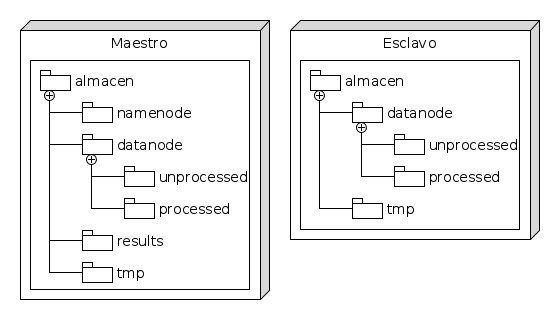
\includegraphics[scale=0.7]{diagramas/esquemahdfs}
\end{figure}

Tras estas decisiones, el esquema resultante es el de la figura \ref{fig:esquemahdfs}. En este podemos apreciar que los nodos contienen las carpetas necesarias para el correcto funcionamiento del \gls{HDFS}. Teniendo el maestro, a parte de la necesaria para controlar el proceso de replicación, la carpeta donde se almacenarán los resultados.

En cuanto a la carga y acceso de los datos de las trazas, veremos en el apartado \ref{sec:implementación}, como las rutas no serán convencionales, como en el diseño del apartado \ref{disNormal}, y se necesitarán unos comandos específicos de \textit{Apache Hadoop} para su manipulación. Con respecto a los resultados, al ser almacenados únicamente en el maestro, si utilizarán el sistema de ficheros del sistema y su comportamiento si que será igual que en el otro diseño.

\subsection{Procesamiento de datos}
Esta unidad funcional será la que se encargue de limpiar las trazas inválidas y transformar los datos de los ficheros que carga el usuario en el sistema. Esta transformación de los datos se da debido a los diferentes requisitos de la competición y se tratará detalladamente durante la implementación del sistema, en el apartado \ref{anaProcData}.

Estará compuesta por una sola clase, escrita en Python, que obtendrá el fichero sin procesar cargado por el usuario en primer lugar y que, tras realizar las transformaciones necesarias lo guardará en el espacio de los archivos procesados, para que pueda ser utilizado por el resto del sistema.

\subsection{Obtención de resultados \label{disConsultas}}
Este bloque de funcionamiento será el encargado de analizar los datos ya procesados y obtener los resultados a la consulta realizada. Estas consultas, que son las establecidas en la competición \cite{grandChallenge}, son las siguientes:

\begin{itemize}
\item \textbf{Rutas más frecuentes:} El objetivo es obtener las diez rutas más frecuentes dentro de la ventana de tiempo establecida entre una fecha y hora dada y la media hora anterior.

\item \textbf{Zonas que más beneficios aportarían al taxista:} El objetivo es obtener las diez zonas de Nueva York donde un taxista obtendría el mayor beneficio empezando un viaje desde allí. Esta consulta también tomaría como entrada una fecha y hora y establecería como ventana de tiempo los 15 minutos anteriores a esta.
\end{itemize}

Estas serían las dos consultas originales de la competición, pero, además, como decisión propia para llevar más al límite a la arquitectura se hicieron modificaciones a estas consultas para tener en cuenta la estacionalidad en los resultados, desarrollando otras dos consultas:

\begin{itemize}
\item \textbf{Rutas más frecuentes teniendo en cuenta la estacionalidad:} El objetivo sigue siendo conseguir las diez rutas más frecuentes pero teniendo en cuenta los viajes de todo el año, dando más importancia a los más cercanos al mes y al día determinado en la consulta. Es decir, esta contará como entrada un mes, un día de la semana y la hora deseada y la consulta obtendrá las rutas más frecuentes teniendo los viajes de todo el año ese día de la semana y a esa hora.

\item \textbf{Zonas que más beneficios aportarían al taxista:} El objetivo es obtener las diez zonas de Nueva York donde un taxista obtendría el mayor beneficio empezando un viaje desde allí. Esta consulta, al igual que la anterior, también tiene en cuenta todos los viajes del año, aunque dando más valor a las fechas cercanas a los argumentos introducidos.
\end{itemize}

Estas consultas, al tener en consideración una franja de tiempo más amplia necesitan más procesamiento para ser calculadas. Además, para aumentar este requerimiento, se ha diseñado para establecer factores de relevancia a los viajes según su cercanía a la fecha introducida.

Por tanto, el sistema contará con la posibilidad de realizar cuatro consultas cuya implementación serán detalladas en el apartado \ref{impConsultas}. El esquema de esta unidad funcional queda representado en la figura \ref{fig:consultas}. 

\begin{figure}[htp!]
\centering
\caption{Esquema de la unidad funcional encargada de realizar las consultas y devolver los resultados}
\label{fig:consultas}
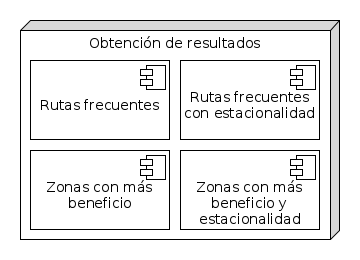
\includegraphics[scale=0.7]{diagramas/obtResultados}
\end{figure}

Con respecto a los resultados de las consultas, estos se guardarán en un archivo con el nombre de la consulta realizada y serán almacenados en la carpeta del almacén de datos destinada para ello, la carpeta ``results''.

\section{Interacciones del sistema}
\begin{figure}[htp!]
\centering
\caption{Componentes e interacciones del sistema \textit{big data}}
\label{fig:interacciones}
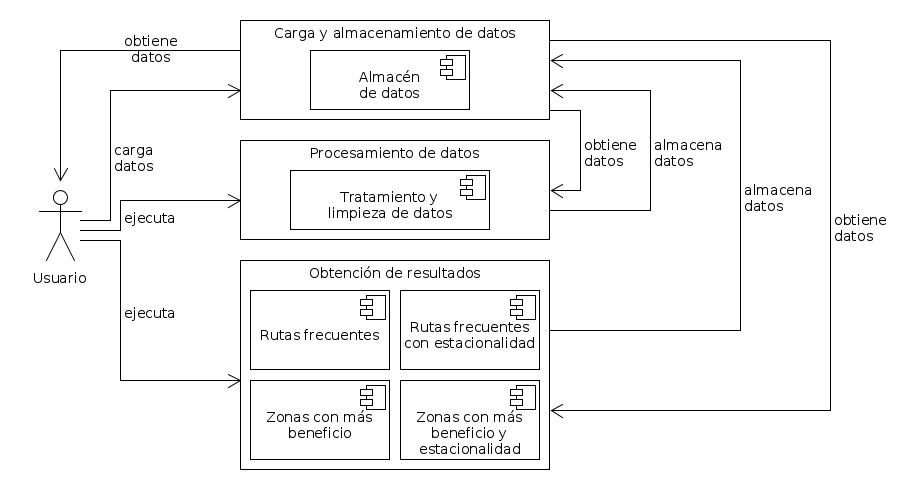
\includegraphics[scale=0.52]{diagramas/interacciones}
\end{figure}

Una vez descritas las diferentes unidades funcionales del sistema y los componentes que las componen, en la figura \ref{fig:interacciones} podemos encontrar un esquema general de las interacciones que se dan entre el usuario y el sistema y, dentro del mismo, entre los diferentes componentes.

En este apartado, además, vamos a detallar las interacciones que se producen al realizar las tareas que la arquitectura puede realizar. Estas tareas son las siguientes: carga de datos en el sistema por parte del usuario, tratamiento y limpieza de los datos, ejecución de las consultas, obtención de los resultados.

\subsection{Carga de datos}
\begin{figure}[htp!]
\centering
\caption{Diagrama de interacción para realizar la carga de los datos}
\label{fig:cargaDatos}
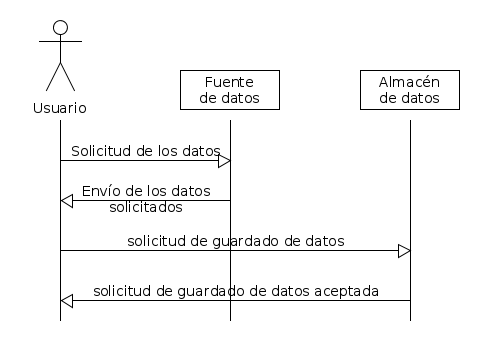
\includegraphics[scale=0.7]{diagramas/cargaDatos}
\end{figure}

Comprende la parte en la que el usuario del sistema carga la traza de taxis, obtenida de la página de la competición. En ella el usuario descarga la traza y la introduce en el sistema mediante su copia en el almacén de datos. Figura \ref{fig:cargaDatos}.

\subsection{Tratamiento y limpieza}

\begin{figure}[htp!]
\centering
\caption{Diagrama de interacción para realizar el tratamiento y la limpieza de los datos}
\label{fig:procesamientoDatos}
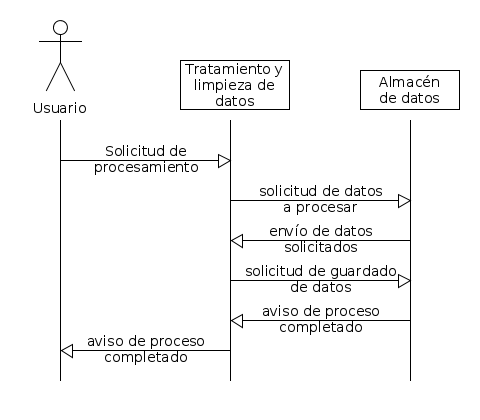
\includegraphics[scale=0.7]{diagramas/procesamientoDatos}
\end{figure}

Este proceso comprende la limpieza y transformación de los datos, procesos necesarios para poder realizar la consulta sobre la traza de datos cargado anteriormente. En este, el usuario realiza una petición de procesamiento al componente con nombre del archivo sin procesar a tratar, que, a su vez, realiza la petición del archivo al almacén de datos. Tras obtener el fichero, este lo trata y realiza el guardado del fichero procesado en el disco, avisando al usuario al finalizar el proceso. Figura \ref{fig:procesamientoDatos}.

\subsection{Ejecución de las consultas}
\begin{figure}[htp!]
\centering
\caption{Diagrama de interacción para realizar las consultas sobre los datos}
\label{fig:consulta}
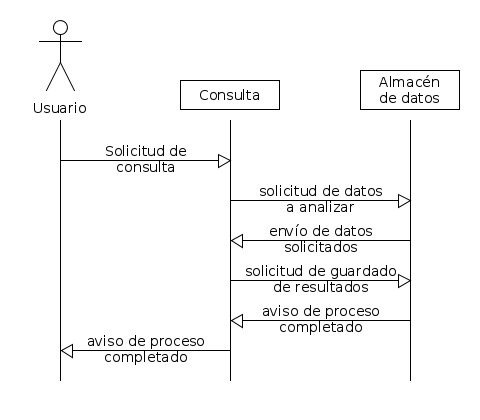
\includegraphics[scale=0.7]{diagramas/consulta}
\end{figure}

Comprende la ejecución de la consulta deseada por el usuario sobre el fichero procesado indicado. Para ello, el usuario realiza una petición al sistema con la consulta que quiere ejecutar y el archivo sobre el que realizarla. Además de indicar los datos requeridos por la consulta. Una vez realizada la petición, el componente de consultas realiza una solicitud al almacén para obtener los datos sobre los que realizará el análisis. Tras realizar el análisis y obtener los resultados, se realiza la petición al almacén para guardarlos y se avisa al usuario de que se ha completado la tarea. Figura \ref{fig:consulta}.

\subsection{Obtención de resultados}
\begin{figure}[htp!]
\centering
\caption{Diagrama de interacción para obterner los resultados de la consulta}
\label{fig:pedirRes}
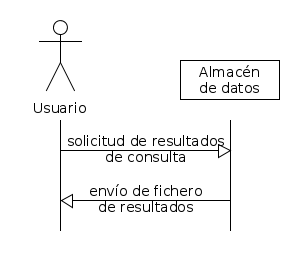
\includegraphics[scale=0.7]{diagramas/pedirRes}
\end{figure}

Este proceso comprende la parte donde el usuario obtiene el fichero de resultados creado tras una consulta ejecutada anteriormente. En este, el usuario realiza una petición al almacén indicando la consulta realizada y este devolverá el fichero con los resultados.


%
% Implementacion
%
\chapter{Implementación\label{sec:implementación}}

\section{Introducción}
En este apartado se detallarán los aspectos relevantes para la implementación de la arquitectura \textit{big data} diseñada en el apartado \ref{sec:disenho}.

Como se indica en dicho apartado, se plantean dos posibles configuraciones para el sistema, el modo pseudo-distribuido, donde solo se utiliza una máquina que hace de maestro y esclavo, y el modo distribuido o multinodo, donde una máquina es el maestro y, el resto, los esclavos. Además, como se ha indicado en el apartado \ref{disMultinodo}, en el caso de la configuración multinodo se implementarán dos diseños diferentes, uno, para el clúster doméstico con un sistema de replicación y, otro, para el clúster universitario que cuenta con un sistema de ficheros en red.

Por tanto, realmente se implementarán tres variaciones del diseño para la arquitectura \textit{big data}, cuya implantación dependerá del entorno:

\begin{itemize}
\item \textbf{Modo pseudo-distribuido:} Se ejecutará tanto en el entorno doméstico como en el universitario, explicado en el apartado \ref{disStandalone}.

\item \textbf{Modo distribuido:} Que tendrá un diseño para cada entorno:

\begin{itemize}
\item \textbf{Clúster doméstico:} Donde se contará con un sistema de replicación de los datos, explicado en el apartado \ref{disDomestico}.
\item \textbf{Clúster universitario:} Donde se cuenta con un sistema de ficheros en red, explicado en el apartado en \ref{disUni}.
\end{itemize}
\end{itemize}

En este apartado, por tanto, se comentarán todos los detalles y pasos necesarios para montar la arquitectura en sus diferentes configuraciones y entornos y, de esta forma, conseguir un sistema \textit{big data} funcional y completo que sea capaz de procesar y analizar los datos para obtener los datos de las consultas planteadas.

Se tratarán los procesos necesarios para lanzar el sistema, desde la instalación del sistema operativo en las máquinas del entorno doméstico, la de \textit{Apache Spark} en todos los nodos, el sistema replicación de \textit{Apache Hadoop} en el clúster doméstico, la configuración de estos sistemas, los procedimientos para la obtención de los datos, el procesado y transformación de los mismos, la implementación de las consultas y hasta la creación y uso de los scripts que hagan funcionar la arquitectura.

\section{Preparación del entorno de trabajo}
Como se expuso en el apartado \ref{sparkEA}, donde se habla de \textit{Apache Spark}, este, resulta compatible con las tres sistemas operativos más importantes para ordenadores, aunque la solución escogida ha sido Linux para ejecutarlo. Utilizando la distribución Ubuntu \cite{ubuntu} en el entorno doméstico y Debian \cite{debian} en el universitario.

La decisión de usar distribuciones basadas en Linux se debieron a varias razones. Primero, porque las máquinas de los laboratorios de la universidad solo vienen equipados con Debian, un \gls{SO} basado en Linux, segundo, por la facilidad y comodidad que ofrece la terminal de Linux, que facilita la ejecución de scripts y la conexión entre los ordenadores a través de \gls{SSH}, tercero, por la mayor cobertura por parte de la documentación oficial y de la comunidad a este \gls{SO} con respecto a \textit{Apache Spark} y, finalmente, porque al tratarse de un proyecto de código abierto, existen distribuciones que no necesitan ningún tipo de licencia, abaratando los costes de la infraestructura.

\subsection{Instalación del sistema operativo}
Esta instalación solo fue necesaria de llevar a cabo en los esclavos que utilizaríamos para el entorno doméstico. Como se ha comentado anteriormente, el \gls{SO} elegido será Ubuntu, concretamente, la versión 16.10.

\subsubsection{Requisitos previos}
Para proceder con la instalación del sistema operativo en los ordenadores había que cumplir algunos requisitos muy básicos. Lo primero era contar con máquinas que superasen los requisitos mínimos \cite{ubuntu} necesarios para su correcta ejecución, cosa que las utilizadas cumplían (especificaciones en el apartado \ref{especifDom}).

También sería necesario un soporte de instalación del \gls{SO}, que en este caso fue un pendrive, con el que se creo una memoria \Gls{USBLive} con Ubuntu, que permitió el inicio de este sistema operativo en las máquinas y su posterior instalación en ellas, de forma local en el disco duro.

\subsubsection{Creación del soporte de instalación}

Para la creación de este \Gls{USBLive} fueron necesarios tres elementos, lo primero, una memoria USB con más de dos gigabytes de espacio disponible, lo segundo una imagen ISO de la instalación de Ubuntu, que obtuvimos de su página oficial \cite{ubuntu} y, por último, la instalación de un programa que cree este tipo de soportes de instalación. En este caso, utilizamos Linux Live USB Creator (LiLi), que facilita en gran manera la tarea formateando e instalando la distribución de forma automática en la memoria USB.

\begin{figure}[htp!]
\centering
\caption{Pantalla principal de Linux Live USB Creator (LiLi)}
\label{fig:lili}
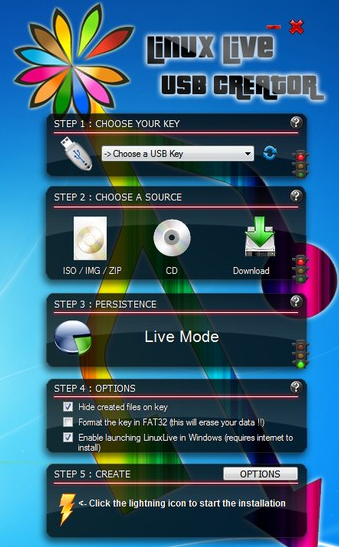
\includegraphics[scale=0.7]{graphics/lili}
\end{figure}

Como vemos en la figura \ref{fig:lili} donde se aprecia la interfaz del programa de creación del \Gls{USBLive} solo hay que seguir los pasos indicados, primero seleccionar el USB deseado, después el fichero del \gls{SO} y, con las opciones por defecto, empezar la instalación pulsando sobre el rayo.

\subsubsection{Instalación de Ubuntu en los nodos}
Para iniciar este proceso lo primero será introducir la memoria \Gls{USBLive} creada en el paso anterior en la máquina deseada y cambiar el orden de arranque de la \gls{BIOS} para que este arranque desde el pendrive insertado.

Una vez arrancado en Ubuntu gracias al soporte, lo siguiente será instalar el \gls{SO} de forma local en el sistema, para ello se procederá de la forma indicada en las instrucciones de instalación, siguiendo los pasos del asistente.

Este proceso lo realizaremos en los nodos que formarán parte del clúster doméstico, en este caso, tres veces y en los tres se hará a partir de este mismo \gls{USBLive}, haciendo que todos corran la misma versión del sistema operativo y evitar incompatibilidades.

\subsection{Instalación de Apache Spark}
Para la realización de este proyecto utilizaremos la versión 2.1 \textit{Apache Spark}, que era la versión disponible cuando se comenzó a trabajar en él. Como lo que se deseaba era una versión estable para realizar todo el trabajo, se descartó la creación del paquete a partir del código fuente y, también, la actualización a la versión 2.1.1 que salió en mayo. 

Por tanto, para la instalación de \textit{Apache Spark} en los equipos que se utilizarían se recurrió a la versión pre-compilada del \Gls{framework}  \cite{descargaSpark}, en concreto la compilada para funcionar con \textit{Apache Hadoop 2.7.3} que se utilizaría en la configuración multinodo del clúster doméstico.

\subsubsection{Prerrequisitos}
Para que \textit{Apache Spark} funcione de forma correcta en el sistema se necesita cumplir una serie de prerrequisitos:

\begin{itemize}
\item Tener instalado Linux en el sistema.
\item Tener instalado Java en el sistema.
\item Tener instalado Scala \cite{scala} en el sistema.
\item Tener instalado Python en el sistema.
\item Tener instalado Py4j \cite{py4j} en el sistema.
\item Tener instalado SSH en el sistema.
\item Disponer de un usuario y grupo común en todas las máquinas.
\end{itemize}

\subsubsection{Instalación de Java y Scala}
La instalación de estos dos lenguajes es esencial para el funcionamiento de \textit{Apache Spark} debido a que está escrito en Scala. Por otro lado, Java es necesario ya que Scala \cite{scala} necesita de la \gls{JVM} para su funcionamiento.

La instalación de estos dos lenguajes de programación se realiza a través de la terminal de forma muy sencilla, poniendo su nombre únicamente, ya que ambas están en el repositorio oficial de Ubuntu. Los comandos necesarios se encuentran en el bloque de código \ref{ins:java}. Con respecto a los equipos de la universidad, estos están ya instalados para su uso.

\begin{lstlisting}[label=ins:java,language=sh,frame=single,caption=Instalación de Java y Scala]
sudo apt update
sudo apt install openjdk-8-jre
sudo apt install scala
\end{lstlisting}

\subsubsection{Instalación de Python y Pyj4}
Python va a ser esencial para el desarrollo de este proyecto ya que se utilizará la \gls{API} en este lenguaje para escribir todo el código que procese \textit{Apache Spark}, conocida como \textit{PySpark}. 

Por otro lado, Pyj4 \cite{py4j} será necesario para la facilitar la comunicación entre el código escrito en Python y Java, ya que su función es facilitar el acceso al intérprete de Python a los objetos de Java que se están ejecutan en la \gls{JVM}.

Python viene instalado por defecto en Ubuntu y Debian por lo que no será necesaria su instalación. Como dato a remarcar, la versión utilizada en este proyecto ha sido la 3.5, debido a ciertas incompatibilidades de la 3.6 con \textit{Apache Spark}.

Con respecto a Py4j, este se instalará a través del \gls{PIP} mediante el comando del bloque de código \ref{ins:py4j}.

\begin{lstlisting}[label=ins:py4j,language=sh,frame=single,caption=Instalación de Py4j]
pip install py4j
\end{lstlisting}

\subsubsection{Creación de usuario y grupo común \label{grupoComun}}
Para evitar posibles problemas de permisos durante la ejecución de las tareas, es buena práctica tener un grupo de usuarios donde estén las máquinas incluidas en el clúster. Esto será necesario únicamente en el entorno doméstico, debido a que en el universitario todos los nodos acceden con el mismo usuario al \gls{NFS}.

Por tanto, para abordar este problema, durante la instalación del \gls{SO} en las máquinas del clúster doméstico se estableció el mismo nombre de usuario para todas. Además, tras esta se creo un nuevo grupo de usuarios, donde se incluyó a dichos usuarios. El proceso para la creación del grupo y adición del usuario a este se puede encontrar en el fragmento de código \ref{usuarioGru}

\begin{lstlisting}[label=usuarioGru,language=sh,frame=single,caption=Creación de grupo común y adición del usuario del sistema a este]
sudo addgroup spark
sudo adduser --ingroup spark adrigrillo
\end{lstlisting}

Una vez realizados estos pasos, las máquinas de la red tendrían acceso a los ficheros de cualquier otra si el grupo tuviese permisos de acceso en dichos archivos. En este caso, todo el conjunto de ficheros utilizados por el sistema \textit{big data} tendrá acceso de lectura y escritura por el grupo de usuarios \textit{spark}, como se explicará en la configuración de \textit{Apache Spark}.

\subsubsection{Instalación de \gls{SSH} y creación del certificado \label{insSSH}}
El cliente de \gls{SSH} viene instalado por defecto en Ubuntu y Debian, sin embargo, para que los nodos devuelvan la llamada del maestro y establecer la conexión cuando se inicie el clúster, será necesario que estos dispongan del servidor \gls{SSH}. 

Estos programas también se encuentran en el repositorio oficial de Ubuntu, por lo que la instalación se realiza escribiendo el nombre del paquete en la terminal. Con respecto a los equipos de la universidad, estos están ya instalados para su uso. El comando de consola para instalarlo se encuentra en el fragmento de código \ref{ins:ssh}.

\begin{lstlisting}[label=ins:ssh,language=sh,frame=single,caption=Instalación del cliente y el servidor de \gls{SSH}]
# En caso de que sea necesario
sudo apt install openssh-client
sudo apt install openssh-server
\end{lstlisting}

Una vez instalados los programas, el siguiente paso será crear el certificado \gls{SSH} para cada equipo y, así, facilitar las conexiones entre los nodos. Es decir, una vez creado los certificados \gls{SSH} de cada máquina, si estos son compartidos entre ellas, los equipos pasarán a estar en la lista de dispositivos seguros y no será necesaria la autentificación con contraseña para establecer la conexión.

El proceso de creación de certificados se puede encontrar en el fragmento de código \ref{confCert} y se realizará en todos las máquinas. Es decir, en el entorno doméstico se creará en cada nodo utilizado, mientras que en el universitario se realizará en una máquina y al contar con un sistema de ficheros en red, pasará a ser válido para todas las demás.

\begin{lstlisting}[label=confCert,language=sh,frame=single,caption=Instalación del cliente y el servidor de \gls{SSH}]
ssh-keygen -t rsa -P ""
cat $HOME/.ssh/id_rsa.pub >> $HOME/.ssh/authorized_keys
\end{lstlisting}

\clearpage
\subsubsection{Instalación y configuración del modo pseudo-distribuido \label{insSparkStand}}
En este modo de ejecución todo el proceso de instalación y configuración se realiza en una sola máquina que hace de maestro y esclavo. Esta implementación, que se realizará en ambos entornos, contará con el mismo proceso para su puesta en marcha, siendo este el descrito posteriormente.

Primero, como hemos indicado al comienzo del apartado, será la descarga de \textit{Apache Spark} desde su página oficial \cite{descargaSpark}, siendo la versión elegida la 2.1 en su modalidad ya precompilada. Tras la descarga, obtendremos el fichero comprimido ``spark-2.1.0-bin-hadoop2.7.tgz'' donde estará todo lo necesario para ejecutar el \gls{framework}.

Aunque por norma general las aplicaciones de este tipo se instalan en la ruta ``/usr/local/'', para este proyecto vamos a crear una estructura de ficheros donde se puedan localizar tantos los programas como los datos a utilizar por el sistema, con el fin de facilitar el manejo de permisos y simplificar la estructura de la arquitectura.

Por tanto, crearemos una carpeta llamada ``big data'' dentro de la carpeta personal del usuario, quedando la ruta siguiente: ``/\$HOME/bigdata/''. Dentro de esta carpeta descomprimiremos el archivo descargado anteriormente y lo renombraremos a ``spark'', situándose en ella la instalación de \textit{Apache Spark}. Por tanto, la ruta de la instalación del \gls{framework} será ``/\$HOME/bigdata/spark''.

En segundo lugar, \textit{Apache Spark} necesita ser configurado para su funcionamiento, teniendo que modificarse diferente ficheros tanto propios como del sistema. 

Lo primero será indicar al sistema la ruta de instalación de \textit{Apache Spark} para que la terminal realice las llamadas a este correctamente. Además, también habrá que indicar la ruta de Java. Estas rutas serán indicadas en el fichero ``.bashrc'' que se localiza en la carpeta personal del usuario del sistema, ``/\$HOME/.bashrc'', quedando el fichero como se indica en el fragmento de código \ref{confBash}.

\begin{lstlisting}[label=confBash,language=sh,frame=single,caption=Líneas a añadir en el fichero ``.bashrc''' para configurar \textit{Apache Spark}]
export SPARK_HOME='/home/adrigrillo/Aplicaciones/spark'
export PATH=$SPARK_HOME:$PATH
export PYTHONPATH=$SPARK_HOME/python:$PYTHONPATH

export JAVA_HOME=/usr/lib/jvm/java-8-openjdk-amd64
export PATH=$PATH:$JAVA_HOME/bin
\end{lstlisting}

Posteriormente, también hay que realizar modificaciones en la configuración de \textit{Apache Spark}. Para ello, será necesario modificar el archivo ``spark-env.sh'' para indicar quien será el maestro del sistema, en este caso la única máquina que lo forma, y para establecer la versión de Python que usará \textit{pyspark}, en este caso la 3.5.

El fichero a modificar se encuentra en ``/\$HOME/bigdata/spark/conf/spark-env.sh'' y las líneas que habrá que añadir se encuentran en el fragmento de código \ref{envStand}.

\begin{lstlisting}[label=envStand,language=sh,frame=single,caption=Líneas a añadir en el fichero ``spark-env.sh'' para configurar \textit{Apache Spark} en el modo pseudo-distribuido]
SPARK_MASTER_HOST=localhost
export PYSPARK_PYTHON=python3
export PYSPARK_DRIVER_PYTHON=/usr/bin/python3
\end{lstlisting}

Tras estos pasos, ya tendríamos lista para funcionar la arquitectura \textit{big data} en modo pseudo-distribuido. 

\subsubsection{Instalación y configuración del modo distribuido}
Este apartado se tratará la configuración de \textit{Apache Spark} para la configuración distribuida o multinodo, donde existe una máquina que hará de maestro y $n$ máquinas que harán de esclavos. 

En este caso, como tenemos dos entornos diferentes para la implementación, el doméstico y el universitario, donde los procesos de instalación y configuración difieren, se indicará en todo momento a cual de las dos configuraciones afecta el proceso realizado.

\paragraph{Asignación de IPs y nombres de sistema en la red}
Este proceso se realizará para simplificar la conexión entre los nodos de los sistemas utilizados, permitiendo con ellos, realizar las conexiones \gls{SSH} mediante el uso de los nombres asignados. 

En el caso del clúster doméstico este proceso se realizará modificando el archivo ``/etc/hosts'' en cada nodo utilizado. Cada equipo recibirá un pseudónimo que corresponderá con su rol, el maestro será \textit{master} y los esclavos serán \textit{esclavo n} donde $n$ será su número de esclavo en el sistema. La modificación del archivo ``hosts'' será la misma para todos los nodos, añadiendo las líneas que se encuentran en el fragmento de código \ref{confhosts}.

\begin{lstlisting}[label=confhosts,language=sh,frame=single,caption=Líneas a añadir en el fichero ``/etc/hosts'' en cada nodo del cúster doméstico]
10.69.186.167 master
10.69.186.122 slave1
10.69.186.178 slave2
\end{lstlisting}

En el caso del clúster universitario, este proceso de modificación del fichero ``hosts'' no será necesario debido a que los nombres de los equipos en la red ya están establecidos de antemano. En este caso, cada máquina tiene un nombre identificativo que bien es ``it0XX'' o ``lm0XX'' donde $XX$ es el número de equipo del laboratorio.

\paragraph{Compartición de certificados \gls{SSH}}
Como se indicó en el apartado \ref{insSSH}, la creación de los certificados \gls{SSH} permitirá que, al compartirse entre los equipos que formen el clúster, no sea necesaria la autentificación con contraseña, simplificando el proceso de conexión entre las máquinas.

En el caso del entorno doméstico, será el maestro el que necesite los certificados de los esclavos para realizar la conexión, por lo que el proceso seguido es la copia de estos en el nodo maestro. El proceso inverso y la compartición entre esclavos no será necesaria, ya que, es el maestro el que inicia la conexión y porque los esclavos no están conectados entre sí.

Los comandos a ejecutar en la terminal del nodo maestro para la obtención de los certificados de los esclavos se puede encontrar en el fragmento de código \ref{comandosSSH}.

\begin{lstlisting}[label=comandosSSH,language=sh,frame=single,caption=Obtención de los certificados \gls{SSH} de los esclavos por parte del maestro en el clúster doméstico]
ssh-copy-id -i $HOME/.ssh/id_rsa.pub adrigrillo@slave1
ssh-copy-id -i $HOME/.ssh/id_rsa.pub adrigrillo@slave2
\end{lstlisting}

En el caso del entorno universitario, al contar con el sistema \gls{NFS} no necesitará de la realización de este proceso. Mediante la creación del certificado \gls{SSH} en la máquina que se utilizará como maestro, realizada en el apartado \ref{insSSH}, este pasa a estar disponible en todas las máquinas conectadas al sistema de ficheros en red, es decir, en los demás nodos que harán de esclavo.

\paragraph{Instalación de \textit{Apache Spark} en el clúster doméstico}
La instalación de \textit{Apache Spark} en este caso se tiene que hacer de forma manual en cada máquina del sistema, al no contarse con un sistema de replicación general (el que se usará solo replicará las trazas) ni un sistema de ficheros en red, como en el clúster universitario.

Para la realización de este proceso de forma automática en cada nodo se creo un script que se ejecutaría en cada nodo del sistema \textit{big data}. El código de este se puede encontrar en el fragmento de código \ref{insSpark}.

\begin{lstlisting}[label=insSpark,language=sh,frame=single,caption=Script de instalación de \textit{Apache Spark} en los nodos del clúster doméstico]
cd /$HOME
mkdir bigdata
cd bigdata/
wget https://d3kbcqa49mib13.cloudfront.net/spark-2.1.0-bin-hadoop2.7.tgz
tar -xvzf spark-2.1.0-bin-hadoop2.7.tgz
mv spark-2.1.0-bin-hadoop2.7 spark
rm -rf spark-2.1.0-bin-hadoop2.7.tgz
\end{lstlisting}

Este proceso, de forma similar a lo realizado de forma manual en la descarga e instalación de \textit{Apache Spark} con la configuración pseudo-distribuida, crea una carpeta ``big data'' en la carpeta del usuario del sistema, descarga la versión precompilada del \gls{framework}, la extrae y la renombrar a ``spark'', pasando este a estar disponible para su ejecución, pasando a estar en la ruta ``/\$HOME/bigdata/spark''.

\clearpage
\paragraph{Instalación de \textit{Apache Spark} en el clúster universitario}
En este caso la descarga e instalación del \gls{framework} sigue el mismo proceso que el realizado en el modo pseudo-distribuido, explicado en el apartado \ref{insSparkStand}, ya que gracias al \gls{NFS}, con realizar la descarga e instalación en un equipo, esta pasará a estar disponible en el resto de nodos.

\paragraph{Configuración de \textit{Apache Spark}}
Los pasos para la configuración en el modo distribuido serán más complejas que en el modo pseudo-distribuido debido a que es necesario establecer los nodos que formarán parte del clúster. Sin embargo, los pasos iniciales de la configuración serán los mismos que en dicho modo (apartado \ref{insSparkStand}), siendo realizados en cada máquina en el caso del clúster doméstico y en una en el clúster universitario.
 
Por tanto, en el entorno doméstico, el primer paso a realizar es indicar al sistema la ruta de instalación de \textit{Apache Spark} y de Java, modificando el archivo ``.bashrc'' de cada nodo. Debido a que el nombre de usuario es el mismo en todos los equipos, el fragmento de código a añadir en el fichero es el mismo para todos, siendo este el que se puede encontrar en el código \ref{confBash}.

Por otro lado, también hay que modificar los archivos de configuración de \textit{Apache Spark} para su correcto funcionamiento. Primero, como en el caso anterior, se modificará el archivo ``spark-env.sh'' en todos los nodos, para establecer que máquina será la maestra y la versión de Python a utilizar.

\begin{lstlisting}[label=envCluster,language=sh,frame=single,caption=Líneas a añadir en el fichero ``spark-env.sh'' para configurar \textit{Apache Spark} en el modo distribuido]
SPARK_MASTER_HOST=master #nombre de red del equipo maestro
export PYSPARK_PYTHON=python3
export PYSPARK_DRIVER_PYTHON=/usr/bin/python3
\end{lstlisting}

Tras realizar esto, el siguiente paso, será establecer que máquinas de la red formarán parte del clúster. Esto se indicará en el archivo ``/\$HOME/bigdata/spark/conf/slaves'', donde se escribirá el nombre de red de los nodos que se utilizarán. En este caso, al ser el clúster doméstico, se utilizarán las tres máquinas disponibles. Las líneas a añadir en el fichero se puede encontrar en el fragmento de código \ref{slavesDom} que solo será necesario escribir en el nodo maestro, que será el que realice las conexiones.

\begin{lstlisting}[label=slavesDom,language=sh,frame=single,caption=Líneas a añadir en el fichero ``slaves'' para establecer las máquinas a utilizar en el clúster doméstico]
master
slave1
slave2
\end{lstlisting}

Con esta configuración realizada, ya tendríamos disponible el clúster doméstico para ser iniciado, aunque no podría realizar ningún trabajo debido a la falta del mecanismo de replicación de datos.

Respecto a la configuración del clúster universitario, el proceso sería muy similar, aunque con pequeñas variaciones. Lo más importante es que la configuración al realizarse en un equipo pasaría a estar disponible en los demás por el \gls{NFS} y, en segundo lugar, las modificaciones con respecto a lo seguido en el clúster doméstico están referidas al nombre de los equipos en la red y el mayor número de configuraciones en la composición del clúster, al contar con diferentes cantidades de nodos.

Por tanto, el proceso de modificación del fichero ``.bashrc'' es igual que en el caso del doméstico pero con las rutas relativas del usuario del laboratorio, sustituyendo ``adrigrillo'' por ``0316457''. En el caso del fichero ``spark-env.sh'' la diferencia reside en el nombre de la máquina que hará de maestro en el clúster, que en este caso será ``lm002''.

La diferencia más notable reside en el fichero ``slaves'' que en el caso del clúster doméstico tendrá varias versiones, con 2, 4, 8 y 16 nodos. Los diferentes ficheros utilizados se puede ver en el anexo \ref{slavesUni}. Por tanto, dependiendo de la configuración con la que se quiera ejecutar el clúster se establecerá uno de los ficheros anteriores.

En este caso, al contar con el sistema de ficheros en red, el clúster ya estaría disponible para su uso sin tener que realizar ninguna configuración más. Únicamente iniciando el clúster como se indicará en el apartado \ref{arranqueSpark}.

\subsection{Instalación de \textit{Apache Hadoop} para el clúster doméstico \label{hadoopClusterDom}}
Como se ha indicado en el diseño de la arquitectura \textit{big data}, en el apartado \ref{sec:disenho}, para la configuración distribuida en el entorno doméstico se necesita un mecanismo de replicación de datos para su funcionamiento. Por tanto, como se explicó, se decidió usar \textit{Apache Hadoop}, en concreto su sistema de ficheros distribuido, \gls{HDFS}, que permitirá la disponibilidad de las trazas en todos los nodos del clúster.

En este apartado se va a proceder a explicar el proceso de instalación y configuración de este sistema. La versión de \textit{Apache Hadoop} utilizada en este proyecto es la versión 2.7.3 precompilada, que está disponible para su descarga desde la página oficial \cite{descHadoop}.

Al tratarse de un sistema distribuido, al igual que con la instalación de \textit{Apache Spark}, esta deberá realizarse en cada sistema. Para agilizar este proceso, se ha creado un script para que realice la descarga del fichero ``.tar.gz'', lo descomprima y lo mueva a la ubicación seleccionada para su instalación. Esta ubicación será similar a la de \textit{Apache Spark}, es decir, será instalado en la ruta ``/\$HOME/bigdata/hadoop/''. El script ejecutado se encuentra en el fragmento de código \ref{insHadoop}.

\begin{lstlisting}[label=insHadoop,language=sh,frame=single,caption=Script de instalación de \textit{Apache Hadoop} en los nodos del clúster doméstico]
cd /$HOME/bigdata/
wget http://apache.rediris.es/hadoop/common/hadoop-2.7.3/hadoop-2.7.3.tar.gz
tar -xvzf hadoop-2.7.3.tar.gz
mv hadoop-2.7.3 hadoop
rm -rf hadoop-2.7.3.tar.gz
\end{lstlisting}

Tras la descarga e instalación de \textit{Apache Hadoop}, para su funcionamiento, será necesario modificar diferentes archivos de configuración. Lo primero será modificar los archivos de sistema para establecer correctamente las rutas de instalación y, posteriormente, los ficheros propios del \gls{framework}.

Como en el caso de la instalación de \textit{Apache Spark} el fichero de sistema a modificar es ``bashrc'', al que habrá que añadirle unas líneas indicando diferentes rutas de instalación de los módulos de \textit{Apache Hadoop} para su funcionamiento. Las lineas a añadir se pueden encontrar en el fragmento de código \ref{bashadoop}.

\begin{lstlisting}[label=bashadoop,language=sh,frame=single,caption=Líneas a añadir a ``.bashrc'' para el funcionamiento de \textit{Apache hadoop}]
export HADOOP_HOME=/home/adrigrillo/Aplicaciones/hadoop
export PATH=$PATH:$HADOOP_HOME/bin
export PATH=$PATH:$HADOOP_HOME/sbin
export HADOOP_MAPRED_HOME=$HADOOP_HOME
export HADOOP_COMMON_HOME=$HADOOP_HOME
export HADOOP_HDFS_HOME=$HADOOP_HOME
export YARN_HOME=$HADOOP_HOME
export HADOOP_COMMON_LIB_NATIVE_DIR=$HADOOP_HOME/lib/native
export HADOOP_OPTS="-Djava.library.path=$HADOOP_HOME/lib"
\end{lstlisting}

Posteriormente, se modificarán los diferentes ficheros de configuración de \textit{Apache Hadoop} para hacerlo funcionar en el clúster doméstico. Todos estos archivos residen en la ruta ``/\$HOME/bigdata/hadoop/etc/hadoop''. Los ficheros a modificar serán los siguientes:

\begin{itemize}
\item \textbf{hadoop-env.sh:} Donde se indicará la ruta de instalación de Java en la máquina.
\begin{lstlisting}[label=hadoopenv,language=sh,frame=single,caption=Línea a añadir a ``hadoop-env.sh'']
export JAVA_HOME=/usr/lib/jvm/java-8-openjdk-amd64
\end{lstlisting}

\item \textbf{core-site.xml}
\begin{lstlisting}[label=coresite,language=XML,frame=single,caption=Líneas a añadir a ``core-site.xml'']
<configuration>
	<property>
	    <name>hadoop.tmp.dir</name>
	    <value>/$HOME/bigdata/almacen/tmp/</value>
	</property> 
	<property>
	    <name>fs.default.name</name>
	    <value>hdfs://master:9000</value> 
	</property>
</configuration>
\end{lstlisting}

\clearpage
\item \textbf{hdfs-site.xml}
\begin{lstlisting}[label=hdfssite1,language=XML,frame=single,caption=Líneas a añadir a ``hdfs-site.xml'' en el nodo maestro]
<configuration>
	<property>
		<name>dfs.replication</name>
		<value>3</value> 
	</property>
	<property>
		<name>dfs.namenode.name.dir</name>
		<value>file:/$HOME/bigdata/almacen/namenode</value>
	</property>
	<property>
		<name>dfs.datanode.data.dir</name>
		<value>file:/$HOME/bigdata/almacen/datanode</value>
	</property>
</configuration>
\end{lstlisting}

\begin{lstlisting}[label=hdfssite2,language=XML,frame=single,caption=Líneas a añadir a ``hdfs-site.xml'' en los nodos esclavos]
<configuration>
	<property>
		<name>dfs.replication</name>
		<value>3</value> 
	</property>
	<property>
		<name>dfs.datanode.data.dir</name>
		<value>file:/$HOME/bigdata/almacen/datanode</value>
	</property>
</configuration>
\end{lstlisting}

\item \textbf{master:} Máquina en la que resida el \textit{namenode}.
\begin{lstlisting}[label=masterHadoop,language=sh,frame=single,caption=Línea a añadir a ``master'']
master
\end{lstlisting}

\item \textbf{slaves:} Máquinas en la que resida el \textit{datanode}, es decir, donde se repliquen los datos.
\begin{lstlisting}[label=slavesHadoop,language=sh,frame=single,caption=Líneas a añadir a ``slaves'']
master
slave1
slave2
\end{lstlisting}
\end{itemize}

Lo que se establece en estos ficheros son, por un lado, los roles de las máquinas implicadas en el clúster y, por otro, las rutas donde se replicarán los datos. Estas rutas coinciden con lo establecido en el diseño, en el apartado \ref{disHDFS}. Es decir, la ruta de la carpeta almacén, donde residirán todos los datos, será ``/\$HOME/bigdata/almacen/'' y, dentro de esta, se localizarán las carpetas como se diseñó en dicho apartado.

\subsection{Estructuración del sistema de ficheros}
Tras los pasos seguidos hasta este apartado, hemos instalado \textit{Apache Spark} para todas las configuraciones de la arquitectura y, para el modo distribuido en el entorno doméstico, también \textit{Apache Hadoop}. Por lo que la estructura de ficheros que encontramos en el sistema es la que se encuentra en la figura \ref{fig:fichAntes}.

\begin{figure}[htp!]
\centering
\caption{Estructura de los ficheros de la arquitectura tras instalación de \textit{Apache Spark} y \textit{Apache Hadoop}}
\label{fig:fichAntes}
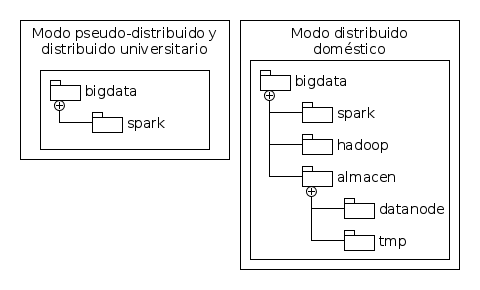
\includegraphics[scale=0.7]{diagramas/fichAntes}
\end{figure}

En este apartado explicaremos la estructuración realizada para establecer una organización clara y sencilla como se estableció en el apartado \ref{diseñoFich} del diseño.

Para ello, en el modo pseudo-distribuido y en el distribuido universitario se establecerá la estructura mostrada en la figura \ref{fig:fichSinRepli}. Para ello se crearán las siguientes carpetas:

\begin{itemize}
\item \textbf{/\$HOME/bigdata/almacen/data/unprocessed/:} donde se cargarán y almacenaran los archivos \gls{CSV} sin procesar.
\item \textbf{/\$HOME/bigdata/almacen/data/processed/:} donde se almacenarán los archivos limpiados y tratados por la arquitectura.
\item \textbf{/\$HOME/bigdata/almacen/results/:} donde se almacenarán los resultados.
\item \textbf{/\$HOME/bigdata/src/:} donde se alojará el código de los componentes del sistema.
\end{itemize}

\begin{figure}[htp!]
\centering
\caption{Estructura de los ficheros para los modos pseudo-distribuido y distribuido universitario}
\label{fig:fichSinRepli}
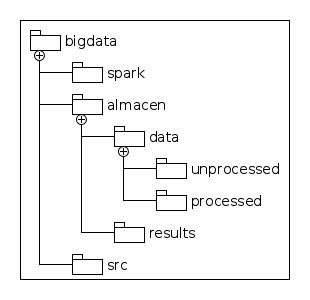
\includegraphics[scale=0.7]{diagramas/fichSinRepli}
\end{figure}

Con respecto al modo distribuido doméstico, al contar con las carpetas necesarias para la replicación de los datos, se establecerá la estructura de la figura \ref{fig:fichConRepli}. Para ello se crearán las siguientes carpetas:

\begin{itemize}
\item \textbf{/\$HOME/bigdata/almacen/results/:} donde se almacenarán los resultados.
\item \textbf{/\$HOME/bigdata/src/:} donde se alojará el código de los componentes del sistema.
\end{itemize}

\begin{figure}[htp!]
\centering
\caption{Estructura de los ficheros para el modos distribuido doméstico}
\label{fig:fichConRepli}
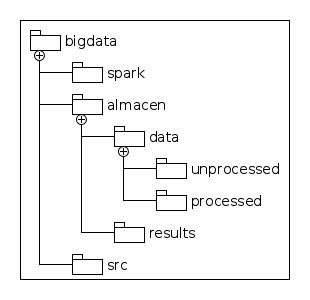
\includegraphics[scale=0.7]{diagramas/fichConRepli}
\end{figure}
 
Para crear las carpetas contenedoras de las trazas de los taxis, al estar estas contenidas dentro del sistema de replicación, será necesarias crearlas mediante los comandos del sistema de ficheros de \textit{Apache Hadoop}. En el fragmento de código \ref{mkdirHDFS} se muestran los comandos necesarios para crear las carpetas ``unprocessed'' y ``processed'' dentro del sistema de replicación.

\begin{lstlisting}[label=mkdirHDFS,language=sh,frame=single,caption=Comandos para crear las carpetas de datos en el \gls{HDFS}]
hdfs namenode -format
hdfs dfs -mkdir /unprocessed
hdfs dfs -mkdir /processed
\end{lstlisting}

Tras la creación de estas carpetas, ya tendremos la estructura de ficheros que la arquitectura utilizará para su funcionamiento.

\subsection{Establecimiento de los permisos para el modo distribuido doméstico}
Para evitar problemas de permisos en la lectura de ficheros, se creó en el apartado \ref{grupoComun}, en esta parte haremos efectiva la creación de este usuario, estableciendo al grupo permisos de lectura y escritura en la estructura de ficheros del sistema en todos los nodos que formen el clúster.

Para ello ejecutaremos el comando escrito en el fragmento de código \ref{permisos} que establecerá los permisos del grupo para la carpeta.

\begin{lstlisting}[label=permisos,language=sh,frame=single,caption=Comando para establecer permisos de lectura y escritura en el sistema de ficheros de la arquitectura]
sudo chown adrigrillo:spark -R /$HOME/bigdata/
\end{lstlisting}

\section{Obtención de las trazas de los taxis y ficheros sin procesar}
El fichero de datos con los viajes de los taxis de la Ciudad de Nueva York es un fichero \gls{CSV} de 33 \gls{GB}. Este fichero, a la fecha en la que se comenzó a trabajar en el proyecto, en febrero de 2017, se podía descargar desde la página de la competición \cite{grandChallenge}, obteniendo así un fichero llamado ``sorted\_data\_full.csv'' que contiene todos los viajes ordenadas por fecha.

Este fichero será introducido en la carpeta de datos sin procesar de la arquitectura y será renombrado a ``full.csv''. Además, a partir de dicho fichero, se crearán más, que sean fragmentos de menor tamaño que este siguiendo lo establecido en la tabla \ref{ficherosCSV}.

Para la creación de los ficheros parciales se utilizará el comando ``head'' de la terminal de Linux, al tratarse reducciones en base al número de registros del fichero original y, cada registro, ocupar una línea, mediante este comando se cogerá el número de líneas indicado desde la primera hasta tal línea y se guardará en el archivo.

\section{Carga de los ficheros en el sistema}
Para la carga de los ficheros creados en el paso anterior distinguiremos entre los dos sistemas de almacenamiento que hemos implementado. Por un lado, tenemos el modo pseudo-distribuido y el distribuido universitario que utilizan el sistema de ficheros del \gls{SO} y, por otro, el sistema distribuido doméstico que hace uso del \gls{HDFS}.

Para el primer grupo, la carga de los ficheros en el sistema se limita a la copia de estos dentro de la carpeta destinada a los ficheros sin procesar, ``/\$HOME/bigdata/almacen/data/unprocessed/''.

Para el modo distribuido, la carga de estos ficheros necesita de los comandos para la gestión del \gls{HDFS}, por tanto, para la carga de los ficheros se utilizará el comando del fragmento de código \ref{cargaFicheroHDFS}. Donde ``ficheroSinProcesar.csv'' será el nombre del fichero a cargar.

\begin{lstlisting}[label=cargaFicheroHDFS,language=sh,frame=single,caption=Comando para añadir los ficheros sin procesar al sistema de replicación]
hdfs dfs -put ficheroSinProcesar.csv unprocessed/
\end{lstlisting}

\section{Análisis y procesamiento de los datos \label{anaProcData}}
En este apartado se va a analizar el fichero de trazas de taxis y se va a describir el proceso de creación del componente de limpieza y tratamiento de los datos. Este componente será el mismo para todas las configuraciones de la arquitectura, es decir, el código será el mismo. Siendo la única diferencia la forma de acceder a los datos en el caso del modo distribuido doméstico.

El siguiente bloque representa un registro de un viaje en el fichero original descargado, que presenta la estructura que se puede apreciar en la tabla \ref{tab:trazaOrig}. 


\begin{verbatim}
07290D3599E7A0D62097A346EFCC1FB5,E7750A37CAB07D0DFF0AF7E3573AC141,
2013-01-01 00:00:00,2013-01-01 00:02:00,120,0.44,-73.956528,40.716976,
-73.962440,40.715008,CSH,3.50,0.50,0.50,0.00,0.00,4.50
\end{verbatim}

\begin{table}[htp!]
\centering
\caption{Campos de la traza de un viaje del fichero original}
\label{tab:trazaOrig}
\begin{tabular}{|l|l|}
\hline
\multicolumn{1}{|c|}{\textbf{NOMBRE}} & \multicolumn{1}{c|}{\textbf{SIGNIFICADO}}                  \\ \hline
medallon                              & Identificador md5sum del taxi                              \\ \hline
licencia                              & Identificador md5sum de la licencia del taxi               \\ \hline
hora\_subida                          & Hora a la que se sube el/la/los/las pasajero/a/os/as       \\ \hline
hora\_bajada                          & Hora a la que se baja el/la/los/las pasajero/a/os/as       \\ \hline
duracion\_viaje\_seg                  & Duración del viaje en segundos                             \\ \hline
distancia\_viaje                      & Distancia del viaje en millas                              \\ \hline
longitud\_subida                      & Coordinada de longitud de la subida                        \\ \hline
latitud\_subida                       & Coordinada de latitud de la subida                         \\ \hline
longitud\_bajada                      & Coordinada de longitud de la bajada                        \\ \hline
latitud\_bajada                       & Coordinada de latitud de la bajada                         \\ \hline
tipo\_pago                            & Método de pago (Tarjeta o efectivo)                        \\ \hline
tarifa                                & Cantidad de la tarifa en dólares                           \\ \hline
recargo                               & Cantidad del recargo en dólares                            \\ \hline
tasas                                 & Cantidad de las tasas en dólares                           \\ \hline
propina                               & Cantidad de la propina en dólares                          \\ \hline
peaje                                 & Cantidad de los peajes de los puentes o tuneles en dólares \\ \hline
cantidad\_total                       & Cantidad total en dólares                                  \\ \hline
\end{tabular}
\end{table}

Primeramente, para facilitar las operaciones posteriormente al trabajar con \textit{Apache Spark}, se establecerá el esquema de la tabla, es decir, los nombres de las columnas expuestos en la tabla \ref{tab:trazaOrig} debido a que los \gls{CSV} aportados no contienen cabeceras. Esto nos permitirá acceder a los atributos de la traza con el nombre a los datos. Para ello, utilizaremos el código escrito en el fragmento \ref{inferSchema}

\begin{lstlisting}[label=inferSchema,language=Python,frame=single,caption=Código para establecer el esquema del \gls{CSV} y facilitar el acceso a los atributos]
nombreColumnas = 
StructType([StructField("medallon", StringType(), True),
StructField("licencia", StringType(), True),
StructField("hora_subida", TimestampType(), True),
StructField("hora_bajada", TimestampType(), True),
StructField("duracion_viaje_seg", IntegerType(), True),
StructField("distancia_viaje", DecimalType(precision=10, scale=2), True),
StructField("longitud_subida", DecimalType(precision=18, scale=14), True),
StructField("latitud_subida", DecimalType(precision=18, scale=14), True),
StructField("longitud_bajada", DecimalType(precision=18, scale=14), True),
StructField("latitud_bajada", DecimalType(precision=18, scale=14), True),
StructField("tipo_pago", StringType(), True),
StructField("tarifa", DecimalType(precision=10, scale=2), True),
StructField("recargo", DecimalType(precision=10, scale=2), True),
StructField("tasas", DecimalType(precision=10, scale=2), True),
StructField("propina", DecimalType(precision=10, scale=2), True),
StructField("peaje", DecimalType(precision=10, scale=2), True),
StructField("cantidad_total", DecimalType(precision=10, scale=2), True)])
\end{lstlisting}

Una vez creado el esquema, este será utilizado en la lectura de los ficheros, al establecerlo como argumento de la función \textit{read}. Por otro lado, para la correcta lectura y trabajo con las fechas, en la misma función, habrá que indicar correctamente el formato de la misma, que en este caso será un string del tipo ``"yyyy-MM-dd HH:mm:ss". Esto nos permitirá la transformación de las fechas en \textit{timestamps} con los que trabajar de forma más cómoda al poder obtener los días de la semana a partir de la fecha o poder sumar y restar en horas, minutos y segundos.

\begin{lstlisting}[label=readCSV,language=python,frame=single,caption=Código para leer los ficheros \gls{CSV}]
""" Lectura de ficheros para los modos pseudo-distribuido
     y distribuido universitario """
data = spark.read.csv("/$HOME/bigdata/almacen/data/unprocessed/nombreFichero.csv", schema=nombreColumnas, timestampFormat="yyyy-MM-dd HH:mm:ss")

""" Lectura de ficheros para el modo distribuido domestico """
data = spark.read.csv("hdfs://master:9000/unprocessed/nombreFichero.csv", schema=nombreColumnas, timestampFormat="yyyy-MM-dd HH:mm:ss")
\end{lstlisting}

En el fragmento de código \ref{readCSV} se encuentra la forma usada para leer los archivos por \textit{Apache Spark} para los dos tipos de almacenamiento que podemos encontrar en el sistema dependiendo de la configuración utilizada.

El primer paso tras introducir los datos en el sistema y ser leídos, es limpiar aquellos registros que no son válidos. En este caso, a parte de los registros que son nulos, debido a que los datos se hayan recogido de forma inválida, la organización del concurso establece un límite de coordenadas para contar el viaje como válido. Es decir, entre las trazas puede haber algún registro cuyas coordenadas se salgan del límite de la ciudad de Nueva York, siendo este inválido. Las coordenadas que limitan el área son:

\begin{itemize}
\item Latitud inicial = 41.477182778
\item Longitud inicial = -74.916578
\item Latitud final = 40,129715978
\item Longitud final = -73.120778
\end{itemize}

Por otro lado, dentro de las trazas existen atributos que no aportan información útil para los posteriores cálculos, atributos como ``distancia\_viaje'', ``recargo'', ``tasas'' o ``peaje''. Estos serán eliminados de todos los registros, ya que, como se va a pasar a un tipo de almacenamiento columnar tras el procesamiento de los datos, es decir, los datos serán guardados en archivos \textit{.parquet}, estos atributos supondrían un gasto en espacio innecesario, ahorrándolo con su supresión.

Por tanto, para la limpieza de los ficheros, aparte de borrar los atributos indicados, se suprimirán los registros en los siguientes casos:

\begin{itemize}
\item Cuando el ID del taxi o de la licencia es nulo.
\item Cuando las horas de subida y bajada coinciden.
\item Cuando la duración del viaje sea igual a 0.
\item Cuando el tipo de pago es diferente a: en efectivo o con tarjeta.
\item Cuando el precio total es igual a 0.
\item Cuando las posiciones de inicio y final son las mismas.
\item Cuando alguna coordenada de posición no esté dentro de los límites de las coordenadas indicadas anteriormente.
\end{itemize}

Debido a la versatilidad de \textit{Apache Spark}, este permite usar lenguaje \gls{SQL} para trabajar con los datos, así como métodos propios. Por tanto, para la limpieza de los datos, realizaremos dos consultas, una para controlar los límites de coordenadas, que utilizará los métodos propios del \gls{framework} para el filtrado debido a la posibilidad de uso de variables globales para usar comparaciones y, otra, que hará el filtrado de las demás condiciones que invalidan un registro, que será en lenguaje \gls{SQL}.

Por tanto, en el fragmento de código \ref{filtroSQL} podemos encontrar la consulta que filtra la mayoría de condiciones y, en el fragmento \ref{filtroLim}, el código que filtra los registros que no están dentro de los límites establecidos.

Una vez realizada la limpieza de los registros, el siguiente paso es hacer el tratamiento de los datos para ajustarse a los requisitos establecidos por la competición. Estos requisitos implican la creación de una cuadrícula con la que dividir la ciudad de Nueva York y poder hacer cálculos desde ella, en vez de usar las coordenadas del fichero original.

Esta cuadrícula tendrá celdas de 500x500 metros y estará compuesta por 300 celdas de ancho por 300 de alto, suponiendo una extensión de 150 kilómetros al este y 150 kilómetros al sur. Para establecer la cuadrícula se da el centro de la primera celda, en la parte superior izquierda, en coordenadas y, a partir de ahí, se establece el resto.

El proceso para la obtención de las coordenadas de cada celda de la cuadrícula se puede encontrar en el anexo \ref{cuadricula}. Sin embargo, para el procesamiento de estos datos, lo que nos interesa es obtener las cuadrículas a la que pertenece cada registro, es decir, a partir de las latitudes y longitudes de subida y bajada del registro, obtener las cuadrículas $(x, y)$ de subida y bajada, pudiendo ser utilizadas para las consultas.

\clearpage
\begin{lstlisting}[label=filtroSQL,language=SQL,frame=single,caption=Filtro de registros en \gls{SQL} para registros inválidos]
SELECT 
    medallon,
    licencia,
    hora_subida,
    hora_bajada,
    duracion_viaje_seg,
    longitud_subida,
    latitud_subida,
    longitud_bajada,
    latitud_bajada,
    tipo_pago,
    tarifa,
    propina,
    cantidad_total
FROM unprocessed 
WHERE   
    medallon <> '' AND 
    licencia <> '' AND
    hora_subida <> hora_bajada AND
    duracion_viaje_seg > 0 AND
    cantidad_total > 0 AND
    longitud_subida <> longitud_bajada AND
    latitud_subida <> latitud_bajada AND
    (tipo_pago == 'CHS' OR tipo_pago == 'CRD')
\end{lstlisting}

\begin{lstlisting}[label=filtroLim,language=python,frame=single,caption=Filtro de coordenadas para los registros que sobrepasan el límite]
data = data.where(data.longitud_subida >= INITIAL_LONGITUDE) \
    .where(data.longitud_subida <= FINAL_LONGITUDE) \
    .where(data.longitud_bajada >= INITIAL_LONGITUDE) \
    .where(data.longitud_bajada <= FINAL_LONGITUDE) \
    .where(data.latitud_subida >= FINAL_LATITUDE) \
    .where(data.latitud_subida <= INITIAL_LATITUDE) \
    .where(data.latitud_bajada >= FINAL_LATITUDE) \
    .where(data.latitud_bajada <= INITIAL_LATITUDE)
\end{lstlisting}

Por tanto, para ello, en los registros se crearán cuatro nuevos atributos, donde se calculará la cuadrícula a partir de las coordenadas. Estos serán:

\begin{itemize}
\item \textbf{cuad\_latitud\_subida:} Que será el valor $x$ de la cuadrícula para la posición de subida del viaje.
\item \textbf{cuad\_longitud\_subida:} Que será el valor $y$ de la cuadrícula para la posición de subida del viaje.
\item \textbf{cuad\_latitud\_bajada:} Que será el valor $x$ de la cuadrícula para la posición de bajada del viaje.
\item \textbf{cuad\_longitud\_bajada:} Que será el valor $y$ de la cuadrícula para la posición de bajada del viaje.
\end{itemize}

Los cálculos de la celda a la que pertenece una coordenada se realiza con las siguientes fórmulas, donde ``INITIAL\_LATITUDE'' e ``INITIAL\_LONGITUDE'' son las coordenadas iniciales de latitud y longitud de la cuadrícula y ``LATITUDE'' y ``LONGITUDE'' son el tamaño de una celda en coordenadas. Las fórmulas son:

\begin{verbatim}
Cuadrícula de latitud =
= int(floor((INITIAL_LATITUDE - latitud_subida)/LATITUDE)) + 1 

Cuadrícula de longitud = 
= int(floor(abs(INITIAL_LONGITUDE - longitud_dada)/LONGITUDE)) + 1
\end{verbatim}

Por otro lado, como en el diseño de las consultas, en el apartado \ref{disConsultas}, se diseñaron dos modificaciones de las originales donde se tenía en cuenta el día de la semana para realizar los cálculos. Esto planteaba dos posibilidades para la implementación, realizar el cálculo del día en la ejecución de la consulta, que implicaría añadir el número de cálculos en cada consulta y cada ejecución, o crear un nuevo atributo en el registro que indicase el día de la semana del viaje, realizando el cálculo una única vez durante el procesamiento y limpieza de los ficheros.

Debido al ahorro en cálculos que esta segunda opción suponía, se tomó este camino, por lo que se crea un nuevo atributo llamado ``dia\_semana''. Para ello se crea una función de usuario para que \textit{Apache Spark} pueda procesar los registros y establecer el resultado de esta en el atributo, esta función se muestra en el código \ref{diaSemana}.

\begin{lstlisting}[label=diaSemana,language=Python,frame=single,caption=Función día de la semana para crear nuevo atributo]
def dia_fecha(fecha):
    return fecha.weekday()

calcular_dia = udf(dia_fecha, IntegerType())
\end{lstlisting}

Por último, tras el tratamiento de los ficheros, el paso final es el guardado de estos ficheros. Para ello, como se ha comentado anteriormente, utilizaremos \textit{Apache Parquet} como formato y \textit{Snappy} como sistema de compresión de los mismos. Esto nos permitirá un ahorro de espacio elevado y una velocidad de procesamiento mayor que utilizando los ficheros \gls{CSV}, como se comprueba en los apartados \ref{compFichDatos} y \ref{resCompFich}.

El almacenamiento se hará en la carpeta ``processed'' de la arquitectura, manteniendo el nombre del fichero original del \gls{CSV}. En el fragmento de código \ref{tratyguardado}, se encuentra el tratamiento de los datos, añadiendo los atributos de la cuadrícula y el día de la semana, y el guardado del fichero resultante.

\clearpage
\begin{lstlisting}[label=tratyguardado,language=Python,frame=single,caption=Código para el tratamiento y guardado del fichero procesado]
""" Establecemos el sistema de cuadriculas y 
calculamos el dia de la semana """
data = data.withColumn("cuad_latitud_subida", floor((INITIAL_LATITUDE - data.latitud_subida)/LATITUDE) + 1) \
    .withColumn("cuad_longitud_subida", floor(abs(INITIAL_LONGITUDE - data.longitud_subida)/LONGITUDE) + 1) \
    .withColumn("cuad_latitud_bajada", floor((INITIAL_LATITUDE - data.latitud_bajada)/LATITUDE) + 1) \
    .withColumn("cuad_longitud_bajada", floor(abs(INITIAL_LONGITUDE - data.longitud_bajada)/LONGITUDE) + 1) \
    .withColumn("dia_semana", CALCULAR_DIA(data.hora_subida))

""" Guardado del fichero en sistema pseudo-distribuido y
	 distribuido universitario """
data.write.option("compression", "snappy") \
        .parquet("/$HOME/bigdata/almacen/data/processed/" + nombre + ".parquet")

""" Guardado del fichero en sistema distribuido domestico """
data.write.option("compression", "snappy") \
        .parquet("hdfs://master:9000/processed/" + nombre + ".parquet")
\end{lstlisting}

\section{Implementación de las consultas \label{impConsultas}}
Como se estableció en el diseño de la arquitectura, apartado \ref{disConsultas}, se establecieron cuatro consultas que el sistema sería capaz de realizar sobre los datos. Dos sobre las rutas más frecuentes y dos sobre las zonas que más beneficios aportarían a los taxistas si iniciasen un viaje desde allí, ambos tipos tienen una consulta donde se tiene en cuenta la estacionalidad y otra donde no.

Estas consultas utilizarán los datos ya procesados anteriormente y que residirán en la carpeta ``processed'', por lo que el primer argumento de todas estas consultas será indicar el fichero sobre el que se trabajará. El resto de argumentos dependerán de la consulta. Tras analizar los datos, el resultado será almacenado en un fichero con el nombre de la consulta, en la carpeta ``results'', donde, aparte del resultado obtenido, se guardará el tiempo de ejecución, que será lo más importante para analizar el sistema posteriormente.

\subsection{Rutas más frecuentes sin estacionalidad \label{freqSinExplicacion}}
El objetivo de esta consulta es obtener las diez rutas más frecuentes durante los 30 minutos anteriores a una fecha y hora establecidas por el usuario, que será el argumento de la consulta. Estas rutas serán válidas únicamente si el viaje ha sido completado, es decir, si el usuario se ha bajado del taxi dentro de la franja del tiempo. 

Por tanto, esta consulta consistirá en dos acciones sobre los datos. Primero, se deberá filtrar los resultados que cumplan con la condición de tiempo, es decir, que hayan acabado dentro de la franja horaria. Posteriormente, se realizará una agrupación por las coordenadas de subida y de bajada y conteo respecto a esta. Es decir, los registros se agruparan en conjuntos que tengan las mismas coordenadas de la cuadrícula de subida y bajada y se contará el número de elementos en cada grupo.

Finalmente, se tomarán los 10 grupos con más registros, y se ordenarán de mayor a menor. El código de la consulta se puede encontrar en el fragmento \ref{codFreq} y la salida de la consulta será la siguiente:

\begin{verbatim}
fecha_subida, fecha_bajada, 0: (celda_subida) (celda_bajada),
1: (celda_subida) (celda_bajada), ..., 9: (celda_subida) (celda_bajada),
tiempo_ejecucion
\end{verbatim}

\begin{lstlisting}[label=codFreq,language=Python,frame=single,caption=Consulta diez rutas más frecuentes]
frequent = data.filter(data.hora_subida <= tiempo_fin) \
        .filter(data.hora_subida >= tiempo_inicio) \
        .filter(data.hora_bajada <= tiempo_fin) \
        .filter(data.hora_bajada >= tiempo_inicio) \
        .groupBy("cuad_longitud_subida", "cuad_latitud_subida", "cuad_longitud_bajada", "cuad_latitud_bajada") \
        .count().orderBy("count", ascending=False)
frequent = frequent.take(10)
\end{lstlisting}

\subsection{Rutas más frecuentes con estacionalidad}
Esta consulta, que es una modificación de la anterior, busca también las diez rutas más frecuentes, pero tiene en cuenta la estacionalidad, es decir, tiene en cuenta el mes en el que se realiza la consulta. Para ello, el usuario introducirá como argumentos el mes, el día de la semana y la hora en la que quiere realizar la consulta.

El sistema, al igual que en la anterior, tomará los viajes que acaben en la media hora anterior a la hora dada, los días de la semana señalados. Además dará un valor mayor a los viajes cercanos al mes indicado y su anterior. Posteriormente, los agrupará por celda de subida y bajada, sumando el valor de la relevancia del viaje y ordenará de mayor a menor con respecto al valor de la misma, devolviendo las diez rutas que mayor valor tengan en el atributo relevancia.

La relevancia de un viaje es 1 por defecto, para simular el valor que tendría en un \textit{count}, sin embargo, si el registro es cercano al mes indicado, pasará a doblar su valor de relevancia, es decir, 2. Un registro es cercano si se encuentra 30 días antes o después del primer día del mes indicado.

Para el funcionamiento de esta consulta se deben crear dos funciones de usuario para que \textit{Apache Spark} pueda utilizarlas en el filtrado de datos, estas serán las que se encuentran en el fragmento \ref{udfFreq}.

\begin{lstlisting}[label=udfFreq,language=Python,frame=single,caption=Funciones de usuario para filtrado de la consulta de rutas frecuentes con estacionalidad]
def comparar_hora(hora):
    """
        Metodo que filtra las horas de los registros para que 
        concuerden con las horas de busqueda deseada
        :param hora: Timestamp completo
        :return: True si las horas del timestamp estan entre las deseadas
        False si lo contrario
    """
    if hora.time() <= HORA_FIN.time() and hora.time() >= HORA_INICIO.time():
        return True
    return False

def relevancia(fecha):
    """
        Metodo que da mas relevancia a los viajes mas cercanos
        a la fecha de busqueda deseada.
        Si la diferencia es menor a un mes de la fecha
        dada los registros tienen mas relevancia
        :param fecha: Timestamp completo
        :return: 2 si el viaje esta cerca de la fecha deseada, 1 si no
    """
    diferencia = fecha - HORA_FIN
    if diferencia < timedelta(days=30) and diferencia > timedelta(days=-30):
        return 2
    else:
        return 1

comprobar_hora = udf(comparar_hora, BooleanType())
calcular_relevancia = udf(relevancia, IntegerType())
\end{lstlisting}

\clearpage
Tras declarar estás funciones, el código de la consulta se puede encontrar en el fragmento \ref{codFreqDay}.

\begin{lstlisting}[label=codFreqDay,language=Python,frame=single,caption=Código consulta de diez rutas más frecuentes teniendo en cuenta la estacionalidad]
""" Devuelve el integer del dia de la semana para filtrar
	 posteriormente los dias que no coinciden con este """
dia_elegido = obtener_dia_semana(DIA_SEMANA)

""" Filtramos los datos con respecto al dia de la semana 
    y la hora.
    Ademas le damos un relevancia a cada viaje
    para el posterior count """
filtered = data.filter(data.dia_semana == dia_elegido) \
	.withColumn("filtroSubida", comprobar_hora(data.hora_subida)) \
	.withColumn("filtroBajada", comprobar_hora(data.hora_bajada)) \
	.withColumn('relevancia', calcular_relevancia(data.hora_subida))

filtered = filtered.filter(filtered.filtroSubida == True) \
    .filter(filtered.filtroBajada == True)

""" Agrupamos por rutas y hacemos el recuento de viajes """
frequent = filtered.groupBy("cuad_longitud_subida", "cuad_latitud_subida", "cuad_longitud_bajada", "cuad_latitud_bajada") \
    .sum("relevancia") \
    .select(col("cuad_longitud_subida"), col("cuad_latitud_subida"), col("cuad_longitud_bajada"), col("cuad_latitud_bajada"), col("sum(relevancia)").alias("frecuencia")) \
    .orderBy("frecuencia", ascending=False)

final = frequent.take(10)
\end{lstlisting}

La salida de esta consulta será muy parecida a la anterior, indicando solo la hora de subida y bajada, siendo la siguiente.

\begin{verbatim}
hora_subida, hora_bajada, 0: (celda_subida) (celda_bajada),
1: (celda_subida) (celda_bajada), ..., 9: (celda_subida) (celda_bajada),
tiempo_ejecucion
\end{verbatim}

\subsection{Zonas que más beneficios proporcionarían al taxista sin estacionalidad \label{profSinExplicacion}}
En esta consulta se busca conseguir las diez zonas, celdas de la cuadrícula, donde el taxista obtendría mayor beneficio empezando un viaje en dicha zona. Para ello, el usuario introducirá como argumento la fecha y la hora sobre la que quiere hacerse la consulta.

El beneficio de una zona se obtiene dividiendo el beneficio obtenido por los taxistas en el conjunto de viajes empezados en dicha zona durante los últimos 15 minutos por la cantidad de taxis vacíos que hay en la zona.

El beneficio que obtiene el taxista con un viaje es la suma de la tarifa y la propina del mismo. Por tanto, el beneficio de una zona, será la media del beneficio de los viajes que han acabado en los últimos 15 minutos y empezaron en esa zona. 

Por tanto, esta consulta se realizará en dos partes, por un lado, se obtendrán el número de taxis libres y, por otro, los beneficios de los taxistas. Posteriormente se unirán los resultados y se realizarán los cálculos para obtener los datos finales y, por tanto, las zonas con más beneficios. La fórmula a aplicar es la siguiente:

\begin{center}
$Beneficio \; zona = \dfrac{media \; de \; tarifa + propina \; (15 \; min)}{taxis \; vacios \; en \; zona \; (30 \; min)}$
\end{center}

\subsubsection{Taxis vacíos en las zonas}
El código de este proceso de la consulta se puede encontrar en el fragmento \ref{taxisVacios}, cuya técnica para obtener los taxis vacíos en una zona durante la última media hora es la siguiente: 

\begin{enumerate}
\item Se obtienen los viajes de subida y bajada de los taxis en la última media hora.

\item Se procede a juntar ambos conjuntos de datos mediante un \textit{join} donde solo los taxis vacíos puedan crear una fila de la tabla. De esta forma se puede comprobar que no se tienen en cuenta los taxis que hayan sido cogidos de nuevo.

\item De esta lista, se eliminan los taxis que hayan sido cogidos tras la ultima bajada, es decir, que hayan iniciado otro viaje durante la ventana de tiempo y no lo haya finalizado.
\end{enumerate}

\clearpage
\begin{lstlisting}[label=taxisVacios,language=Python,frame=single,caption=Código para obtener los taxis vacíos en las zonas de la ciudad durante la última media hora]
# Obtenemos los ultimos viajes de subida y bajada de los taxis
bajadas30 = tripsDown \
    .select("medallon", "hora_bajada", "cuad_latitud_bajada", "cuad_longitud_bajada") \
    .orderBy("hora_bajada", ascending=False) \
    .dropDuplicates(subset=["medallon"])

subidas30 = tripsUp \
    .select("medallon", "hora_subida").orderBy("hora_subida", ascending=False) \
    .dropDuplicates(subset=["medallon"]).withColumnRenamed("medallon", "taxi")

""" Procedemos a juntar ambos conjuntos de datos para asi
    poder comprobar que no se tienen en cuenta los taxis
    que hayan sido cogidos de nuevo """
# Spark falla join si el nombre de la columna es el mismo,
# renombrado a taxi
joined = bajadas30.join(subidas30, bajadas30.medallon == subidas30.taxi, "leftouter") \
    .select("medallon", "hora_bajada", "hora_subida", "cuad_latitud_bajada", "cuad_longitud_bajada")

# Eliminamos los taxis que hayan sido cogidos tras la ultima bajada
estado_taxis = joined.select(joined.medallon, joined.cuad_latitud_bajada, joined.cuad_longitud_bajada, when(joined.hora_subida > joined.hora_bajada, 1).otherwise(0).alias("taxi_ocupado"))
    
taxis_filtrados = estado_taxis.filter(estado_taxis.taxi_ocupado == 0)

taxis_libres = taxis_filtrados.groupBy("cuad_latitud_bajada", "cuad_longitud_bajada").count() \
   .select(col("cuad_latitud_bajada"), col("cuad_longitud_bajada"), col("count").alias("taxis_libres"))
\end{lstlisting}

\clearpage
\subsubsection{Beneficio de las zonas}
El código de este fragmento se puede encontrar en el fragmento \ref{beneficioZona}. Para obtener estos datos, los pasos a seguir son los siguientes:

\begin{enumerate}
\item Se realiza un filtrado tomando los viajes acabados en los últimos 15 minutos.
\item Estos viajes son agrupados por la celda en la que son iniciados.
\item Se calcula la media de la tarifa y de la propina de cada zona establecida en el agrupamiento.
\item Se realiza la suma de la media de la tarifa y de la propina para cada zona, obteniéndose así el beneficio medio de las zonas.
\end{enumerate}

\begin{lstlisting}[label=beneficioZona,language=Python,frame=single,caption=Código para obtener el beneficio de las zonas de la ciudad durante los últimos quince minutos]
beneficios = trips15.groupBy("cuad_latitud_subida", "cuad_longitud_subida") \
    .avg("tarifa", "propina") \
    .select(col("cuad_latitud_subida"), col("cuad_longitud_subida"), \ col("avg(tarifa)") + col("avg(propina)")).alias("beneficios"))
\end{lstlisting}

\subsubsection{Obtención del beneficio proporcionado para el taxista}
Tras obtener los datos necesarios para obtener el beneficio real de la zona, el siguiente paso es unirlos y operar sobre ellos. Para ello, lo primero es realizar el \textit{join} de las dos tablas. En este caso, la única tabla que creará filas será la tabla de beneficio medio de las zonas, debido a que nos interesa evitar los cálculos de zonas donde no hay datos de beneficio pero existen taxis libres.

Tras la unión de estas dos tablas, se creará un nuevo atributo, llamado ``beneficio'' que será el resultado de la división del beneficio medio de la zona entre el número de taxis libres en dicha zona. Para evitar las divisiones por 0 cuando no hay taxis libres en la zona, se ha sumado 1 a la cuenta de los taxis libres. De esta forma, cuando no hay taxis se obtiene el beneficio integro de la zona y cuando hay algún taxista, se obtiene la repartición de beneficios.

La salida de esta consulta serán las diez zonas que más beneficios aportarían al taxista durante la ventana de tiempo introducida. Esta será la siguiente:

\begin{verbatim}
fecha_subida, fecha_bajada, 0: (celda_zona), 1: (celda_zona), ..., 
9: (celda_zona), tiempo_ejecucion
\end{verbatim}

El código de la unión de estas dos tablas y obtención de los resultados es el escrito en el fragmento \ref{unioProfi}.

\begin{lstlisting}[label=unioProfi,language=Python,frame=single,caption=Código de la unión de tablas de beneficios y taxis libres y obtención de los resultados de la consulta]
condicion = [beneficios.cuad_latitud_subida == taxis_libres.cuad_latitud_bajada, beneficios.cuad_longitud_subida == taxis_libres.cuad_longitud_bajada]

profitable = beneficios \
    .join(taxis_libres, condicion, "leftouter") \
    .select(col("cuad_latitud_subida").alias("cuad_latitud"), col("cuad_longitud_subida").alias("cuad_longitud"), (col("beneficios") / when(taxis_libres.taxis_libres > 0, (taxis_libres.taxis_libres + 1)).otherwise(1)).alias("beneficio")) \
    .orderBy("beneficio", ascending=False)

profitable = profitable.take(10)
\end{lstlisting}

\subsection{Zonas que más beneficios proporcionarían al taxista con estacionalidad}
Esta consulta que es una modificación de la anterior, tiene el mismo objetivo que esta, obtener las diez zonas que más beneficios puede procurar al taxista. En esta, como en el caso de las rutas frecuentes con estacionalidad, tiene en cuenta el mes introducido para obtener los resultados.

Por tanto, el usuario introducirá como argumentos el mes, el día de la semana y la hora en la que quiere realizar la consulta. El sistema, realizará los mismos cálculos que la consulta original, sin embargo, la diferencia está en que se aplicará un factor de influencia a los registros dependiendo de la cercanía de la fecha del registro al mes deseado por el usuario.

Este factor de influencia se utilizará tanto sobre el número de taxis libres como el valor de los beneficios medios de las zonas. Este factor se aplicará mediante la creación de una función de usuario de \textit{Apache Spark}, escrito en el fragmento de código \ref{infProf}.

Además, al no utilizar \textit{timestamps} completos en esta consulta, también se han de crear dos funciones de usuario para filtrar los registros por tiempo. Estas serán las escritas en el código \ref{ufTiempo}.

\clearpage
\begin{lstlisting}[label=infProf,language=Python,frame=single,caption=Función de usuario para aplicar el factor de relevancia]
def relevancia(fecha):
    """
        Metodo que da mas relevancia a los viajes mas cercanos
        a la fecha de busqueda deseada.
        Si la diferencia es menor a un mes de la fecha
        dada los registros tienen mas relevancia
        :param fecha: Timestamp completo
        :return: 2 si el viaje esta cerca de la fecha deseada, 1 si no
    """
    diferencia = fecha - HORA_FIN
    if diferencia < timedelta(days=7) and diferencia > timedelta(days=-7):
        return 1.0
    elif diferencia < timedelta(days=14) and diferencia > timedelta(days=-14):
        return 0.75
    elif diferencia < timedelta(days=21) and diferencia > timedelta(days=-21):
        return 0.5
    elif diferencia < timedelta(days=-28) and diferencia > timedelta(days=-28):
        return 0.25
    else:
        return 0

calcular_relevancia = udf(relevancia, FloatType())
\end{lstlisting}

\begin{lstlisting}[label=ufTiempo,language=Python,frame=single,caption=Funciones de usuario para filtrar los registros por tiempo]
def comparar_media_hora(hora):
    """
        Metodo que filtra las horas de los registros para que concuerden
        con las horas de busqueda deseada
        :param hora: Timestamp completo
        :return: True si las horas del timestamp estan entre las deseadas
        False si lo contrario
    """
    if hora.time() <= HORA_FIN.time() and hora.time() >= HORA_30.time():
        return True
    return False


def comparar_cuarto_hora(hora):
    """
        Metodo que filtra las horas de los registros para que concuerden
        con las horas de busqueda deseada
        :param hora: Timestamp completo
        :return: True si las horas del timestamp estan entre las deseadas
        False si lo contrario
    """
    if hora.time() <= HORA_FIN.time() and hora.time() >= HORA_15.time():
        return True
    return False

comprobar_media_hora = udf(comparar_media_hora, BooleanType())
comprobar_cuarto_hora = udf(comparar_cuarto_hora, BooleanType())
\end{lstlisting}

El código de esta consulta es el escrito en el fragmento de código \ref{codProfDay}. La salida de esta consulta serán las diez zonas que más beneficios aportarían al taxista durante la ventana de tiempo introducida, en el día de la semana introducido. Esta será la siguiente:

\begin{verbatim}
hora_subida, hora_bajada, 0: (celda_zona), 1: (celda_zona), ..., 
9: (celda_zona), tiempo_ejecucion
\end{verbatim}

\begin{lstlisting}[label=codProfDay,language=Python,frame=single,caption=Código de la consulta para obtener las diez zonas que proporcionan más beneficios al taxista teniendo en cuenta la estacionalidad]
dia_elegido = obtener_dia_semana(DIA_SEMANA)

# Filtramos los datos con respecto al dia de la semana y la hora
trips_down = data.filter(data.dia_semana == dia_elegido) \
    .filter(comprobar_media_hora(data.hora_bajada))

trips_up = data.filter(data.dia_semana == dia_elegido) \
    .filter(comprobar_media_hora(data.hora_subida))

# Borramos duplicados y los ordenamos por proximidad 
# a la hora deseada
down_30_min = trips_down.select("medallon", "hora_bajada", "cuad_latitud_bajada", "cuad_longitud_bajada") \
    .orderBy("hora_bajada", ascending=False) \
    .dropDuplicates(subset=["medallon"])



up_30_min = trips_up.select("medallon", "hora_subida").orderBy("hora_subida", ascending=False) \
    .dropDuplicates(subset=["medallon"]).withColumnRenamed("medallon", "taxi")

# spark falla join si el nombre de la columna es el mismo,
# renombrado a taxi
joined = down_30_min.join(up_30_min, down_30_min.medallon == up_30_min.taxi, "leftouter") \
    .select("medallon", "hora_bajada", "hora_subida", "cuad_latitud_bajada", "cuad_longitud_bajada")

# Sacamos los taxis que estan libres con su posicion
estado_taxis = joined.select(joined.medallon, joined.cuad_latitud_bajada, joined.cuad_longitud_bajada, joined.hora_bajada, when(joined.hora_subida > joined.hora_bajada, 1).otherwise(0).alias("taxi_ocupado"))

# Anyadimos el factor de influencia a cada taxi
# segun la distancia a fecha del registro
taxis_filtrados = estado_taxis.filter(estado_taxis.taxi_ocupado == 0) \
    .withColumn("influencia", calcular_relevancia(estado_taxis.hora_bajada))

# Calculamos el numero de taxis vacios en las zonas
taxis_libres = taxis_filtrados.groupBy("cuad_latitud_bajada", "cuad_longitud_bajada").count() \
    .select(col("cuad_latitud_bajada"), col("cuad_longitud_bajada"), col("count").alias("taxis_libres"))

# Calculamos la influencia de la zona con la media
# de la influencia de los taxis en dicha zona
influencia_taxis_libres = taxis_filtrados \
    .groupBy("cuad_latitud_bajada", "cuad_longitud_bajada") \
    .avg("influencia") \
    .select(col("cuad_latitud_bajada").alias("latitud"), col("cuad_longitud_bajada").alias("longitud"), col("avg(influencia)").alias("influencia"))

""" Calculamos la proporcion de taxis libres por zona, 
    esta proporcion es el numero de taxis libres en la 
    zona por la influencia de estos taxis.
    Siendo menos influyentes cuanto mas alejados
    en el tiempo """
condition = [taxis_libres.cuad_latitud_bajada == influencia_taxis_libres.latitud, taxis_libres.cuad_longitud_bajada == influencia_taxis_libres.longitud]

taxis_libres_prop = taxis_libres.join(influencia_taxis_libres, condition) \
    .select(col("cuad_latitud_bajada"), col("cuad_longitud_bajada"), round(col("taxis_libres") * col("influencia")).alias("proporcion_taxis_libres"))

"""
    PASAMOS A LOS BENEFICIOS
"""
# Filtramos viajes por tiempo y anyadimos influencia con
# respecto a la fecha deseada
trips_15 = trips_down.filter(comprobar_cuarto_hora(data.hora_bajada)) \
    .withColumn("influencia", calcular_relevancia(estado_taxis.hora_bajada))

# Obtenemos los beneficios de la zona con la influencia
# tenida en cuenta
beneficios = trips_15.groupBy("cuad_latitud_subida", "cuad_longitud_subida") \
    .avg("tarifa", "propina", "influencia") \
    .select(col("cuad_latitud_subida"), col("cuad_longitud_subida"), col("avg(tarifa)") + col("avg(propina)")) * col("avg(influencia)")).alias("beneficios"))

# Unimos los beneficios con los taxis libres y dividimo
# beneficios/taxis_libres
condicion = [beneficios.cuad_latitud_subida == taxis_libres.cuad_latitud_bajada, beneficios.cuad_longitud_subida == taxis_libres.cuad_longitud_bajada]

profitable = beneficios.join(taxis_libres_prop, condicion, "leftouter") \
    .select(col("cuad_latitud_subida").alias("cuad_latitud"), col("cuad_longitud_subida").alias("cuad_longitud"), col("beneficios") / col("proporcion_taxis_libres")).alias("beneficio")) \
    .orderBy("beneficio", ascending=False)

# Obtenemos el top 10
profitable = profitable.take(10)
\end{lstlisting}


%
% Uso del sistema
%
\chapter{Uso del sistema \label{sec:usodelsistema}}
Este apartado esta destinado a explicar los pasos y comandos necesarios para poner en marcha el sistema \textit{bigdata} implementado en el apartado \ref{sec:implementación} y poder utilizarlo. Por tanto, se explicarán los scripts y comandos necesarios para realizar la conexión de los nodos y establecimiento de los clúster, así como los necesarios para ejecutar las funciones del sistema y, finalmente, se analizarán los scripts utilizados para realizar las pruebas.

\section{Arranque de las máquinas}
En este apartado hay que diferenciar entre los dos modos de ejecución disponibles, el modo pseudo-distribuido y el distribuido. Para el primero, este paso solo consiste en el encendido de la máquina a utilizar.

En el caso del segundo, el proceso es más complejo, ya que, además de encender cada uno de los nodos, hay que comprobar que su conexión a la red es correcta, es decir, se tiene que verificar que el equipo esté conectado a la red y que la configuración de las direcciones IP y los nombres de red es correcto.

Además, en este segundo caso, también hay que comprobar que las conexiones \gls{SSH} se realizan correctamente entre los nodos.

\section{Arranque de \textit{Apache Spark} \label{arranqueSpark}}
Este paso solo será necesario realizarlo en el caso de los sistemas distribuidos, ya que el modo pseudo-distribuido solo contiene un nodo, por lo que no hay que establecer ningún tipo de conexión, necesitando solo el envío de un trabajo para su funcionamiento.

En el caso del modo multinodo, el proceso de inicialización de \textit{Apache Spark} se realiza ejecutando un script contenido en la carpeta donde está instalado el \gls{framework}. Este ejecutable, que se encuentra en la ruta ``\$HOME/bigdata/spark/sbin/start-all.sh'', será el encargado de realizar las conexiones con los nodos esclavos y arrancar la interfaz web de \textit{Apache Spark}, que se puede apreciar en la figura \ref{fig:interfazSpark}.

Este script se ejecutará desde el nodo maestro. En cuanto a la interfaz web, nos permitirá comprobar que todos los nodos están conectados correctamente y, además, el estado de los trabajos que está realizando o ha realiza el sistema.

\begin{figure}[htp!]
\centering
\caption{Interfaz web de \textit{Apache Spark}}
\label{fig:interfazSpark}
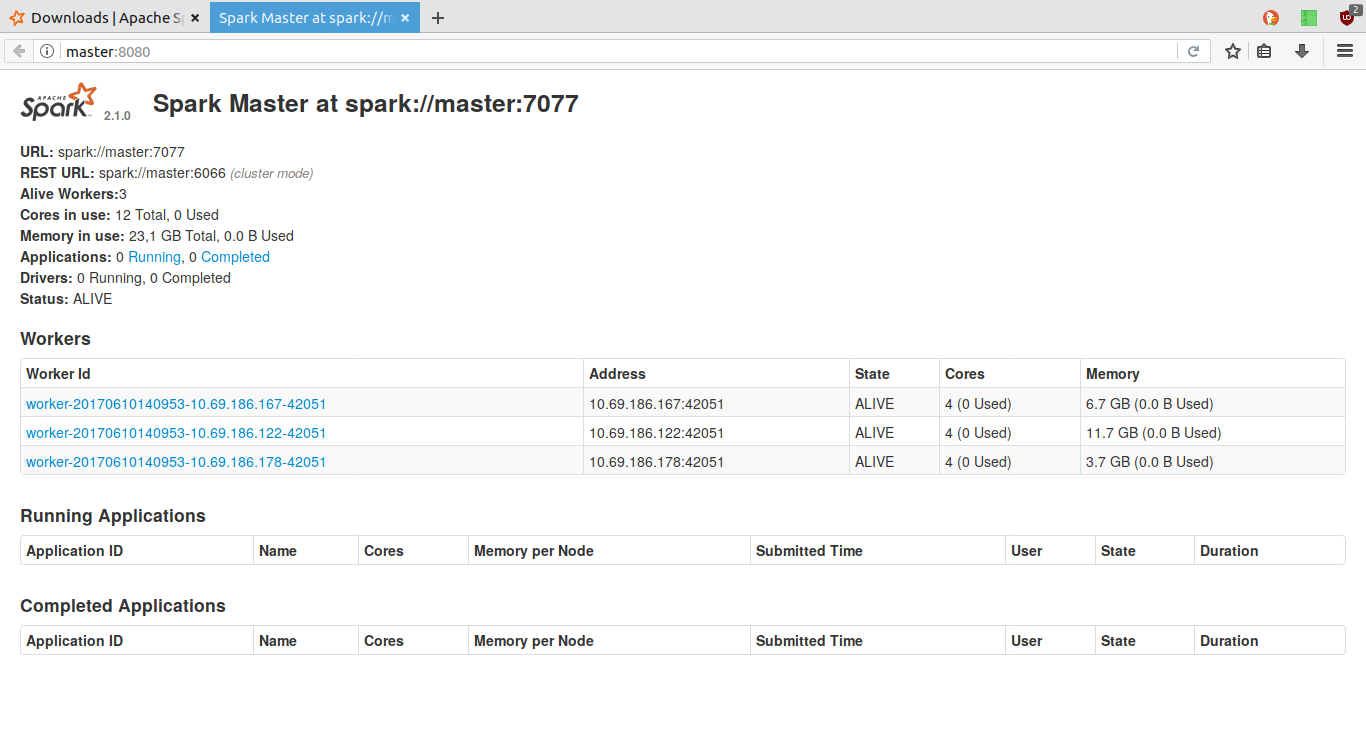
\includegraphics[scale=0.3]{graphics/clusterDom}
\end{figure}

\section{Arranque de \textit{Apache Hadoop}}
Como se indicó en los apartados \ref{disDomestico} y \ref{hadoopClusterDom}, la arquitectura \textit{big data} contará con el sistema de replicación de \textit{Apache Hadoop} únicamente en la configuración multinodo doméstica. En este apartado, se tratará el arranque y parada del \gls{HDFS}, además de otros comandos para su manipulación.

De forma muy similar a \textit{Apache Spark}, el arranque del sistema de replicación se realiza mediante un script que está contenido en la carpeta de instalación, en la ruta ``/\$HOME/bigdata/hadoop/sbin/start-dfs.sh''. Este ejecutable se encarga de arrancar del sistema de replicación en todos los nodos, realizando la transmisión de los datos si es necesario desde el maestro a los nodos.

Para parar el sistema, también se cuenta con un script encargado de detener el sistema de replicación y realizar la desconexión entre los equipos. Este se encuentra en ``/\$HOME/bigdata/hadoop/sbin/start-dfs.sh''. Con respecto al resto de comandos, estos se comentarán en el fragmento de código \ref{comandosHDFS}.

\begin{lstlisting}[label=comandosHDFS,language=sh,frame=single,caption=Comandos \textit{Apache Hadoop}]
# Formatear sistema de replicacion
hdfs namenode -format

# Crear carpeta en el sistema
hdfs dfs -mkdir /nombreCarpeta

# Copiar desde local al sistema de replicacion
hdfs dfs -put /rutaLocal /rutaHDFS

# Eliminar archivo o carpeta del sistema de replicacion
hdfs dfs -rmr /rutaParaEliminar
\end{lstlisting}

Este sistema de replicación también contará con una interfaz web que alojará el nodo maestro, en ella se podrá comprobar el estado de cada nodo y navegar por el sistema de ficheros. Ambas funciones se pueden apreciar en las figuras \ref{fig:compHadoop} y \ref{fig:fichHadoop}.

\begin{figure}[htp!]
\centering
\caption{Interfaz web de \textit{Apache Hadoop} con el estado de los nodos}
\label{fig:compHadoop}
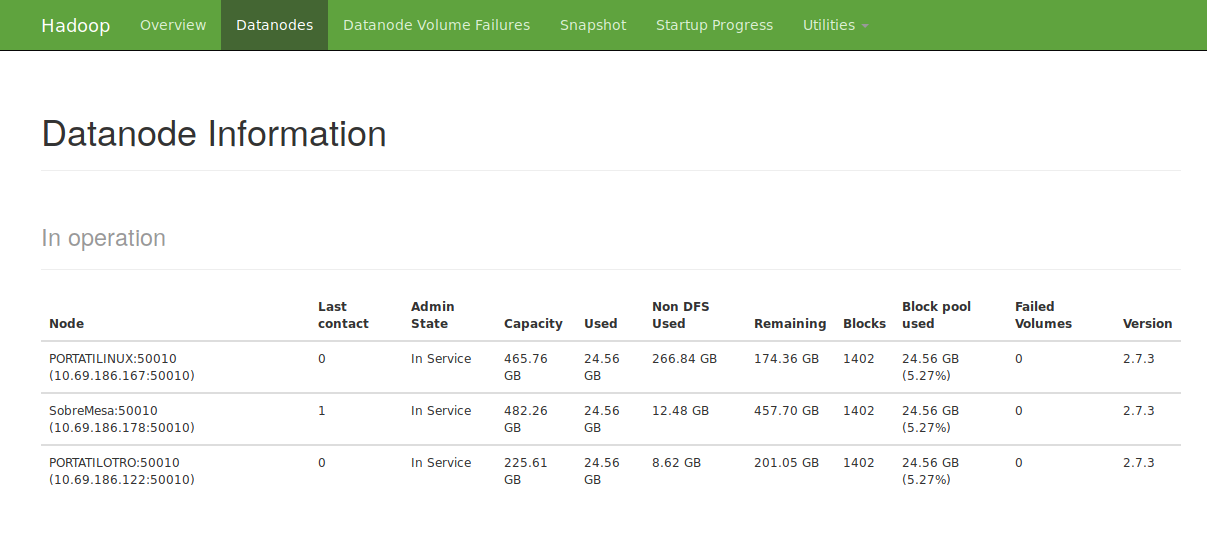
\includegraphics[scale=0.35]{graphics/hadoopDatanode}
\end{figure}

\begin{figure}[htp!]
\centering
\caption{Interfaz web de \textit{Apache Hadoop} con el navegador del sistema de ficheros}
\label{fig:fichHadoop}
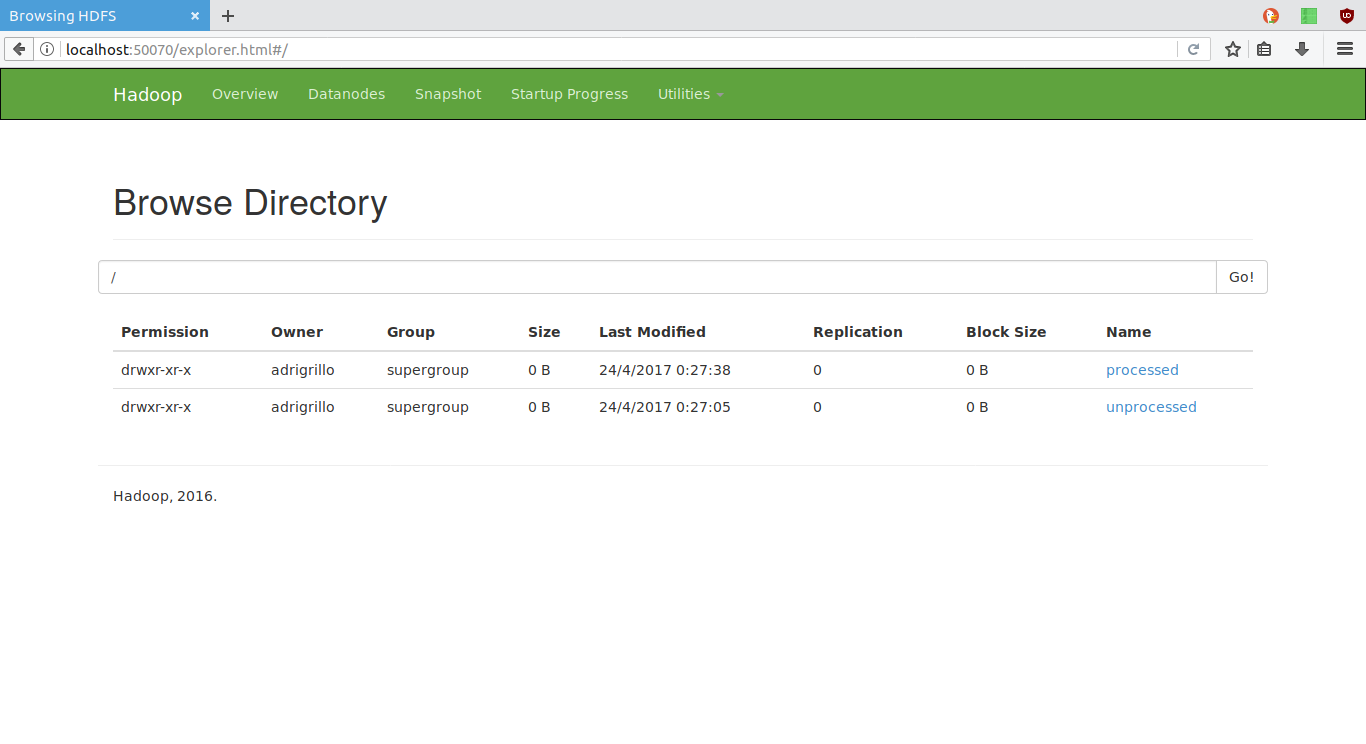
\includegraphics[scale=0.35]{graphics/directorioHadoop}
\end{figure}

\section{Ejecución de trabajos en \textit{Apache Spark}}
Para ejecutar un trabajo de \textit{Apache Spark} se utilizará el script ``spark-submit'' que es el que se encargará de gestionar el proceso. Este ejecutable se localiza en la ruta ``/\$HOME/bigdata/spark/bin/spark-submit'' y, entre otros argumentos \cite{submitSpark}, hay que introducir la clase con el código del trabajo a ejecutar y, si es necesario, la dirección web del maestro del clúster, para que este reparta el trabajo. En el fragmento de código \ref{submits} se mostrará la forma de enviar un trabajo dependiendo de la configuración de la arquitectura.

\begin{lstlisting}[label=submits,language=sh,frame=single,caption=Comando para el envío de un trabajo a \textit{Apache Spark} dependiendo del modo de ejecución de la arquitectura \textit{big data}]
# Submit en el modo pseudo-distribuido
/$HOME/bigdata/spark/bin/spark-submit fichero.py

# Submit en el modo distribuido
/$HOME/bigdata/spark/bin/spark-submit --master spark://nombreRedMaestro:7077 fichero.py
\end{lstlisting}


\section{Ejecución del procesado de datos}
El componente del procesado de los datos está contenido en la clase ``DataProcessing.py'', que se encuentra en la carpeta destinada al guardado del código fuente y los scripts, en la ruta ``/\$HOME/bigdata/src/DataProcessing.py''.

Esta clase será la encargada de la limpieza y el tratamiento de los registros, como se ha explicado en el apartado \ref{anaProcData}. Este fichero se ejecutará desde la terminal y tomará tres argumentos para su correcto funcionamiento, que serán los siguientes:

\begin{itemize}
\item \textbf{Fichero:} Fichero de datos sin procesar sobre los que trabajar. Este nombre tiene que coincidir con algún fichero de la carpeta ``unprocessed'', sin introducir la extensión \textit{*.csv}.
\item \textbf{Nombre:} Nombre del archivo con el que se desea guardar el resultado del procesamiento, en general, se utilizará el nombre del fichero a procesar.
\item \textbf{Tiempos:} Nombre con el que se desea guardar el archivo que contendrá el tiempo de procesamiento de la ejecución.
\end{itemize}

\section{Ejecución de las consultas}
Los ficheros que contienen el código de las consultas, al igual que el fichero de procesamiento, se encuentran en la ruta ``/\$HOME/bigdata/src/''. En este caso, para cada consulta habrá una clase de Python, estas serán:

\begin{itemize}
\item \textbf{FrequentRoutes.py:} Rutas más frecuentes sin estacionalidad. Los argumentos de entrada son:
\begin{enumerate}
\item \textbf{Fichero:} Fichero sobre el que se realizará la consulta, coincidente con alguno de la carpeta ``processed''.
\item \textbf{Fecha:} Día, mes y año sobre el que se trabajará, \textit{string} con el formato ``aaaa-mm-dd''.
\item \textbf{Hora:} Hora y minutos sobre la que establecer la ventana de tiempo, \textit{string} con el formato ``HH:MM''.
\end{enumerate}

\clearpage
\item \textbf{FrequentRoutesDay.py:} Rutas más frecuentes con estacionalidad.
\begin{enumerate}
\item \textbf{Fichero:} Fichero sobre el que se realizará la consulta, coincidente con alguno de la carpeta ``processed''.
\item \textbf{Mes:} Nombre del mes al que se le quiere dar más valor para calcular la influencia de los registros.
\item \textbf{Día de la semana:} Día de la semana sobre la que se trabajará.
\item \textbf{Hora:} Hora y minutos sobre la que establecer la ventana de tiempo, \textit{string} con el formato ``HH:MM''.
\end{enumerate}

\item \textbf{ProfitableAreas.py:} Zonas que más beneficios proporcionarían al taxista sin estacionalidad.
\begin{enumerate}
\item \textbf{Fichero:} Fichero sobre el que se realizará la consulta, coincidente con alguno de la carpeta ``processed''.
\item \textbf{Fecha:} Día, mes y año sobre el que se trabajará, \textit{string} con el formato ``aaaa-mm-dd''.
\item \textbf{Hora:} Hora y minutos sobre la que establecer la ventana de tiempo, \textit{string} con el formato ``HH:MM''.
\end{enumerate}

\item \textbf{ProfitableAreasDay.py:} Zonas que más beneficios proporcionarían al taxista con estacionalidad
\begin{enumerate}
\item \textbf{Fichero:} Fichero sobre el que se realizará la consulta, coincidente con alguno de la carpeta ``processed''.
\item \textbf{Mes:} Nombre del mes al que se le quiere dar más valor para calcular la influencia de los registros.
\item \textbf{Día de la semana:} Día de la semana sobre la que se trabajará.
\item \textbf{Hora:} Hora y minutos sobre la que establecer la ventana de tiempo, \textit{string} con el formato ``HH:MM''.
\end{enumerate}
\end{itemize}

\section{Scripts ejecutables de las pruebas}
En este apartado se describirán los scripts realizados para las pruebas realizadas en el sistema. Estas pruebas, que se analizan en el apartado \ref{sec:resultados}, consisten en la ejecución de forma repetida, de los cinco elementos ejecutables del sistema, la limpieza y tratamiento de los datos y las cuatro consultas.

Por tanto, el apartado se dividirá en cinco subapartados donde se mostrarán los scripts ejecutados, tanto para el modo pseudo-distribuido como para el multinodo.

\subsection{Procesamiento de datos}

\begin{lstlisting}[label=sproc,language=sh,frame=single,caption=Script procesamiento de datos en modo pseudo-distribuido]
 Procesamiento del csv de forma local
/$HOME/bigdata/spark/bin/spark-submit DataProcessing.py mil.csv mil mil
/$HOME/bigdata/spark/bin/spark-submit DataProcessing.py quinientos.csv quinientos quinientos
/$HOME/bigdata/spark/bin/spark-submit DataProcessing.py cinquenta.csv cinquenta cinquenta
/$HOME/bigdata/spark/bin/spark-submit DataProcessing.py 1decimo.csv 1decimo 1decimo
/$HOME/bigdata/spark/bin/spark-submit DataProcessing.py 2decimo.csv 2decimo 2decimo
/$HOME/bigdata/spark/bin/spark-submit DataProcessing.py 3decimo.csv 3decimo 3decimo
/$HOME/bigdata/spark/bin/spark-submit DataProcessing.py 4decimo.csv 4decimo 4decimo
/$HOME/bigdata/spark/bin/spark-submit DataProcessing.py half.csv half half
/$HOME/bigdata/spark/bin/spark-submit DataProcessing.py 6decimo.csv 6decimo1 6decimo
/$HOME/bigdata/spark/bin/spark-submit DataProcessing.py 7decimo.csv 7decimo1 7decimo
/$HOME/bigdata/spark/bin/spark-submit DataProcessing.py 8decimo.csv 8decimo1 8decimo
/$HOME/bigdata/spark/bin/spark-submit DataProcessing.py 9decimo.csv 9decimo1 9decimo
/$HOME/bigdata/spark/bin/spark-submit DataProcessing.py full.csv full1 full
\end{lstlisting}

\begin{lstlisting}[label=sprocDis,language=sh,frame=single,caption=Script procesamiento de datos en modo distribuido]
 Procesamiento del csv de forma local
/$HOME/bigdata/spark/bin/spark-submit --master spark://master:7077 DataProcessing.py mil.csv mil mil
/$HOME/bigdata/spark/bin/spark-submit --master spark://master:7077 DataProcessing.py quinientos.csv quinientos quinientos
/$HOME/bigdata/spark/bin/spark-submit --master spark://master:7077 DataProcessing.py cinquenta.csv cinquenta cinquenta
/$HOME/bigdata/spark/bin/spark-submit --master spark://master:7077 DataProcessing.py 1decimo.csv 1decimo 1decimo
/$HOME/bigdata/spark/bin/spark-submit --master spark://master:7077 DataProcessing.py 2decimo.csv 2decimo 2decimo
/$HOME/bigdata/spark/bin/spark-submit --master spark://master:7077 DataProcessing.py 3decimo.csv 3decimo 3decimo
/$HOME/bigdata/spark/bin/spark-submit --master spark://master:7077 DataProcessing.py 4decimo.csv 4decimo 4decimo
/$HOME/bigdata/spark/bin/spark-submit --master spark://master:7077 DataProcessing.py half.csv half half
/$HOME/bigdata/spark/bin/spark-submit --master spark://master:7077 DataProcessing.py 6decimo.csv 6decimo1 6decimo
/$HOME/bigdata/spark/bin/spark-submit --master spark://master:7077 DataProcessing.py 7decimo.csv 7decimo1 7decimo
/$HOME/bigdata/spark/bin/spark-submit --master spark://master:7077 DataProcessing.py 8decimo.csv 8decimo1 8decimo
/$HOME/bigdata/spark/bin/spark-submit --master spark://master:7077 DataProcessing.py 9decimo.csv 9decimo1 9decimo
/$HOME/bigdata/spark/bin/spark-submit --master spark://master:7077 DataProcessing.py full.csv full1 full
\end{lstlisting}

\subsection{Rutas más frecuentes sin estacionalidad}
\begin{lstlisting}[label=sfreq,language=sh,frame=single,caption=Script rutas más frecuentes sin estacionalidad en modo pseudo-distribuido]
/$HOME/bigdata/spark/bin/spark-submit FrequentRoutes.py mil.parquet 2013-01-01 09:45
/$HOME/bigdata/spark/bin/spark-submit FrequentRoutes.py quinientos.parquet 2013-01-01 09:45
/$HOME/bigdata/spark/bin/spark-submit FrequentRoutes.py cinquenta.parquet 2013-01-01 09:45
/$HOME/bigdata/spark/bin/spark-submit FrequentRoutes.py 1decimo.parquet 2013-01-01 09:45
/$HOME/bigdata/spark/bin/spark-submit FrequentRoutes.py 2decimo.parquet 2013-01-01 09:45
/$HOME/bigdata/spark/bin/spark-submit FrequentRoutes.py 3decimo.parquet 2013-01-01 09:45
/$HOME/bigdata/spark/bin/spark-submit FrequentRoutes.py 4decimo.parquet 2013-01-01 09:45
/$HOME/bigdata/spark/bin/spark-submit FrequentRoutes.py half.parquet 2013-01-01 09:45
/$HOME/bigdata/spark/bin/spark-submit FrequentRoutes.py 6decimo.parquet 2013-01-01 09:45
/$HOME/bigdata/spark/bin/spark-submit FrequentRoutes.py 7decimo.parquet 2013-01-01 09:45
/$HOME/bigdata/spark/bin/spark-submit FrequentRoutes.py 8decimo.parquet 2013-01-01 09:45
/$HOME/bigdata/spark/bin/spark-submit FrequentRoutes.py 9decimo.parquet 2013-01-01 09:45
/$HOME/bigdata/spark/bin/spark-submit FrequentRoutes.py full.parquet 2013-01-01 09:45
\end{lstlisting}
\begin{lstlisting}[label=sfreqdis,language=sh,frame=single,caption=Script rutas más frecuentes sin estacionalidad en modo distribuido]
/$HOME/bigdata/spark/bin/spark-submit --master spark://master:7077 FrequentRoutes.py mil.parquet 2013-01-01 09:45
/$HOME/bigdata/spark/bin/spark-submit --master spark://master:7077 FrequentRoutes.py quinientos.parquet 2013-01-01 09:45
/$HOME/bigdata/spark/bin/spark-submit --master spark://master:7077 FrequentRoutes.py cinquenta.parquet 2013-01-01 09:45
/$HOME/bigdata/spark/bin/spark-submit --master spark://master:7077 FrequentRoutes.py 1decimo.parquet 2013-01-01 09:45
/$HOME/bigdata/spark/bin/spark-submit --master spark://master:7077 FrequentRoutes.py 2decimo.parquet 2013-01-01 09:45
/$HOME/bigdata/spark/bin/spark-submit --master spark://master:7077 FrequentRoutes.py 3decimo.parquet 2013-01-01 09:45
/$HOME/bigdata/spark/bin/spark-submit --master spark://master:7077 FrequentRoutes.py 4decimo.parquet 2013-01-01 09:45
/$HOME/bigdata/spark/bin/spark-submit --master spark://master:7077 FrequentRoutes.py half.parquet 2013-01-01 09:45
/$HOME/bigdata/spark/bin/spark-submit --master spark://master:7077 FrequentRoutes.py 6decimo.parquet 2013-01-01 09:45
/$HOME/bigdata/spark/bin/spark-submit --master spark://master:7077 FrequentRoutes.py 7decimo.parquet 2013-01-01 09:45
/$HOME/bigdata/spark/bin/spark-submit --master spark://master:7077 FrequentRoutes.py 8decimo.parquet 2013-01-01 09:45
/$HOME/bigdata/spark/bin/spark-submit --master spark://master:7077 FrequentRoutes.py 9decimo.parquet 2013-01-01 09:45
/$HOME/bigdata/spark/bin/spark-submit --master spark://master:7077 FrequentRoutes.py full.parquet 2013-01-01 09:45
\end{lstlisting}

\subsection{Rutas más frecuentes con estacionalidad}
\begin{lstlisting}[label=sfreqday,language=sh,frame=single,caption=Script rutas más frecuentes con estacionalidad en modo pseudo-distribuido]
/$HOME/bigdata/spark/bin/spark-submit FrequentRoutesDay.py mil.parquet martes 01-01 11:00
/$HOME/bigdata/spark/bin/spark-submit FrequentRoutesDay.py quinientos.parquet martes 01-01 11:00
/$HOME/bigdata/spark/bin/spark-submit FrequentRoutesDay.py cinquenta.parquet martes 01-01 11:00
/$HOME/bigdata/spark/bin/spark-submit FrequentRoutesDay.py 1decimo.parquet martes 01-01 11:00
/$HOME/bigdata/spark/bin/spark-submit FrequentRoutesDay.py 2decimo.parquet martes 01-01 11:00
/$HOME/bigdata/spark/bin/spark-submit FrequentRoutesDay.py 3decimo.parquet martes 01-01 11:00
/$HOME/bigdata/spark/bin/spark-submit FrequentRoutesDay.py 4decimo.parquet martes 01-01 11:00
/$HOME/bigdata/spark/bin/spark-submit FrequentRoutesDay.py half.parquet martes 01-01 11:00
/$HOME/bigdata/spark/bin/spark-submit FrequentRoutesDay.py 6decimo.parquet martes 01-01 11:00
/$HOME/bigdata/spark/bin/spark-submit FrequentRoutesDay.py 7decimo.parquet martes 01-01 11:00
/$HOME/bigdata/spark/bin/spark-submit FrequentRoutesDay.py 8decimo.parquet martes 01-01 11:00
/$HOME/bigdata/spark/bin/spark-submit FrequentRoutesDay.py 9decimo.parquet martes 01-01 11:00
/$HOME/bigdata/spark/bin/spark-submit FrequentRoutesDay.py full.parquet martes 01-01 11:00
\end{lstlisting}
\begin{lstlisting}[label=sfreqdaydis,language=sh,frame=single,caption=Script rutas más frecuentes con estacionalidad en modo distribuido]
/$HOME/bigdata/spark/bin/spark-submit --master spark://master:7077 FrequentRoutesDay.py mil.parquet martes 01-01 11:00
/$HOME/bigdata/spark/bin/spark-submit --master spark://master:7077 FrequentRoutesDay.py quinientos.parquet martes 01-01 11:00
/$HOME/bigdata/spark/bin/spark-submit --master spark://master:7077 FrequentRoutesDay.py cinquenta.parquet martes 01-01 11:00
/$HOME/bigdata/spark/bin/spark-submit --master spark://master:7077 FrequentRoutesDay.py 1decimo.parquet martes 01-01 11:00
/$HOME/bigdata/spark/bin/spark-submit --master spark://master:7077 FrequentRoutesDay.py 2decimo.parquet martes 01-01 11:00
/$HOME/bigdata/spark/bin/spark-submit --master spark://master:7077 FrequentRoutesDay.py 3decimo.parquet martes 01-01 11:00
/$HOME/bigdata/spark/bin/spark-submit --master spark://master:7077 FrequentRoutesDay.py 4decimo.parquet martes 01-01 11:00
/$HOME/bigdata/spark/bin/spark-submit --master spark://master:7077 FrequentRoutesDay.py half.parquet martes 01-01 11:00
/$HOME/bigdata/spark/bin/spark-submit --master spark://master:7077 FrequentRoutesDay.py 6decimo.parquet martes 01-01 11:00
/$HOME/bigdata/spark/bin/spark-submit --master spark://master:7077 FrequentRoutesDay.py 7decimo.parquet martes 01-01 11:00
/$HOME/bigdata/spark/bin/spark-submit --master spark://master:7077 FrequentRoutesDay.py 8decimo.parquet martes 01-01 11:00
/$HOME/bigdata/spark/bin/spark-submit --master spark://master:7077 FrequentRoutesDay.py 9decimo.parquet martes 01-01 11:00
/$HOME/bigdata/spark/bin/spark-submit --master spark://master:7077 FrequentRoutesDay.py full.parquet martes 01-01 11:00
\end{lstlisting}

\subsection{Zonas que más beneficios proporcionarían al taxista sin estacionalidad}
\begin{lstlisting}[label=sprof,language=sh,frame=single,caption=Script onas que más beneficios proporcionarían al taxista sin estacionalidad en modo pseudo-distribuido]
/$HOME/bigdata/spark/bin/spark-submit ProfitableAreas.py mil.parquet 2013-01-01 09:45
/$HOME/bigdata/spark/bin/spark-submit ProfitableAreas.py quinientos.parquet 2013-01-01 09:45
/$HOME/bigdata/spark/bin/spark-submit ProfitableAreas.py cinquenta.parquet 2013-01-01 09:45
/$HOME/bigdata/spark/bin/spark-submit ProfitableAreas.py 1decimo.parquet 2013-01-01 09:45
/$HOME/bigdata/spark/bin/spark-submit ProfitableAreas.py 2decimo.parquet 2013-01-01 09:45
/$HOME/bigdata/spark/bin/spark-submit ProfitableAreas.py 3decimo.parquet 2013-01-01 09:45
/$HOME/bigdata/spark/bin/spark-submit ProfitableAreas.py 4decimo.parquet 2013-01-01 09:45
/$HOME/bigdata/spark/bin/spark-submit ProfitableAreas.py half.parquet 2013-01-01 09:45
/$HOME/bigdata/spark/bin/spark-submit ProfitableAreas.py 6decimo.parquet 2013-01-01 09:45
/$HOME/bigdata/spark/bin/spark-submit ProfitableAreas.py 7decimo.parquet 2013-01-01 09:45
/$HOME/bigdata/spark/bin/spark-submit ProfitableAreas.py 8decimo.parquet 2013-01-01 09:45
/$HOME/bigdata/spark/bin/spark-submit ProfitableAreas.py 9decimo.parquet 2013-01-01 09:45
/$HOME/bigdata/spark/bin/spark-submit ProfitableAreas.py full.parquet 2013-01-01 09:45
\end{lstlisting}
\clearpage
\begin{lstlisting}[label=sprofdis,language=sh,frame=single,caption=Script onas que más beneficios proporcionarían al taxista sin estacionalidad en modo distribuido]
/$HOME/bigdata/spark/bin/spark-submit --master spark://master:7077 ProfitableAreas.py mil.parquet 2013-01-01 09:45
/$HOME/bigdata/spark/bin/spark-submit --master spark://master:7077 ProfitableAreas.py quinientos.parquet 2013-01-01 09:45
/$HOME/bigdata/spark/bin/spark-submit --master spark://master:7077 ProfitableAreas.py cinquenta.parquet 2013-01-01 09:45
/$HOME/bigdata/spark/bin/spark-submit --master spark://master:7077 ProfitableAreas.py 1decimo.parquet 2013-01-01 09:45
/$HOME/bigdata/spark/bin/spark-submit --master spark://master:7077 ProfitableAreas.py 2decimo.parquet 2013-01-01 09:45
/$HOME/bigdata/spark/bin/spark-submit --master spark://master:7077 ProfitableAreas.py 3decimo.parquet 2013-01-01 09:45
/$HOME/bigdata/spark/bin/spark-submit --master spark://master:7077 ProfitableAreas.py 4decimo.parquet 2013-01-01 09:45
/$HOME/bigdata/spark/bin/spark-submit --master spark://master:7077 ProfitableAreas.py half.parquet 2013-01-01 09:45
/$HOME/bigdata/spark/bin/spark-submit --master spark://master:7077 ProfitableAreas.py 6decimo.parquet 2013-01-01 09:45
/$HOME/bigdata/spark/bin/spark-submit --master spark://master:7077 ProfitableAreas.py 7decimo.parquet 2013-01-01 09:45
/$HOME/bigdata/spark/bin/spark-submit --master spark://master:7077 ProfitableAreas.py 8decimo.parquet 2013-01-01 09:45
/$HOME/bigdata/spark/bin/spark-submit --master spark://master:7077 ProfitableAreas.py 9decimo.parquet 2013-01-01 09:45
/$HOME/bigdata/spark/bin/spark-submit --master spark://master:7077 ProfitableAreas.py full.parquet 2013-01-01 09:45
\end{lstlisting}

\subsection{Zonas que más beneficios proporcionarían al taxista con estacionalidad}
\begin{lstlisting}[label=sprofday,language=sh,frame=single,caption=Script onas que más beneficios proporcionarían al taxista con estacionalidad en modo pseudo-distribuido]
/$HOME/bigdata/spark/bin/spark-submit ProfitableAreasDay.py mil.parquet martes 01-01 11:00
/$HOME/bigdata/spark/bin/spark-submit ProfitableAreasDay.py quinientos.parquet martes 01-01 11:00
/$HOME/bigdata/spark/bin/spark-submit ProfitableAreasDay.py cinquenta.parquet martes 01-01 11:00
/$HOME/bigdata/spark/bin/spark-submit ProfitableAreasDay.py 1decimo.parquet martes 01-01 11:00
/$HOME/bigdata/spark/bin/spark-submit ProfitableAreasDay.py 2decimo.parquet martes 01-01 11:00
/$HOME/bigdata/spark/bin/spark-submit ProfitableAreasDay.py 3decimo.parquet martes 01-01 11:00
/$HOME/bigdata/spark/bin/spark-submit ProfitableAreasDay.py 4decimo.parquet martes 01-01 11:00
/$HOME/bigdata/spark/bin/spark-submit ProfitableAreasDay.py half.parquet martes 01-01 11:00
/$HOME/bigdata/spark/bin/spark-submit ProfitableAreasDay.py 6decimo.parquet martes 01-01 11:00
/$HOME/bigdata/spark/bin/spark-submit ProfitableAreasDay.py 7decimo.parquet martes 01-01 11:00
/$HOME/bigdata/spark/bin/spark-submit ProfitableAreasDay.py 8decimo.parquet martes 01-01 11:00
/$HOME/bigdata/spark/bin/spark-submit ProfitableAreasDay.py 9decimo.parquet martes 01-01 11:00
/$HOME/bigdata/spark/bin/spark-submit ProfitableAreasDay.py full.parquet martes 01-01 11:00
\end{lstlisting}

\begin{lstlisting}[label=sprofdaydis,language=sh,frame=single,caption=Script onas que más beneficios proporcionarían al taxista con estacionalidad en modo distribuido]
/$HOME/bigdata/spark/bin/spark-submit --master spark://master:7077 ProfitableAreasDay.py mil.parquet martes 01-01 11:00
/$HOME/bigdata/spark/bin/spark-submit --master spark://master:7077 ProfitableAreasDay.py quinientos.parquet martes 01-01 11:00
/$HOME/bigdata/spark/bin/spark-submit --master spark://master:7077 ProfitableAreasDay.py cinquenta.parquet martes 01-01 11:00
/$HOME/bigdata/spark/bin/spark-submit --master spark://master:7077 ProfitableAreasDay.py 1decimo.parquet martes 01-01 11:00
/$HOME/bigdata/spark/bin/spark-submit --master spark://master:7077 ProfitableAreasDay.py 2decimo.parquet martes 01-01 11:00
/$HOME/bigdata/spark/bin/spark-submit --master spark://master:7077 ProfitableAreasDay.py 3decimo.parquet martes 01-01 11:00
/$HOME/bigdata/spark/bin/spark-submit --master spark://master:7077 ProfitableAreasDay.py 4decimo.parquet martes 01-01 11:00
/$HOME/bigdata/spark/bin/spark-submit --master spark://master:7077 ProfitableAreasDay.py half.parquet martes 01-01 11:00
/$HOME/bigdata/spark/bin/spark-submit --master spark://master:7077 ProfitableAreasDay.py 6decimo.parquet martes 01-01 11:00
/$HOME/bigdata/spark/bin/spark-submit --master spark://master:7077 ProfitableAreasDay.py 7decimo.parquet martes 01-01 11:00
/$HOME/bigdata/spark/bin/spark-submit --master spark://master:7077 ProfitableAreasDay.py 8decimo.parquet martes 01-01 11:00
/$HOME/bigdata/spark/bin/spark-submit --master spark://master:7077 ProfitableAreasDay.py 9decimo.parquet martes 01-01 11:00
/$HOME/bigdata/spark/bin/spark-submit --master spark://master:7077 ProfitableAreasDay.py full.parquet martes 01-01 11:00
\end{lstlisting}

%
% Resultados
%
\chapter{Pruebas y resultados\label{sec:resultados}}

\section{Introducción}
Tras el diseño y la implementación del sistema \textit{big data}, se procederá con la realización de conjuntos de baterías de pruebas en los diferentes entornos con el fin de estudiar su escalabilidad, comparar su rendimiento y detectar limitaciones del sistema. 

Estas pruebas se realizarán teniendo en cuenta dos factores, por un lado, el tamaño del fichero a procesar, es decir, partiendo del archivo completo se generarán otros ficheros parciales de menor tamaño con el objetivo de detectar el umbral donde el uso de un sistema distribuido pasa a ser efectivo. Por otro lado, utilizaremos distintas configuraciones del sistema para comparar su eficiencia, variando el número de procesadores (\gls{CPU}) y la cantidad de \gls{RAM}.

Estas pruebas serán complementarias, es decir, se realizarán para todos los sistemas de forma simultánea. Con respecto a las configuraciones del sistema \textit{big data} diseñadas, para realizar las pruebas, utilizaremos dos de ellas. Primero estableceremos el sistema en modo pseudo-distribuido y, posteriormente, en modo multinodo. Estas, se realizaran tanto en el clúster doméstico como en el universitario.

\section{Entorno de prueba}
En este apartado se detallarán las características de las máquinas utilizadas para cada configuración del sistema \textit{big data}.

\subsection{Configuración pseudo-distribuida}
En este modo solo existe una máquina que ejerce como maestro y esclavo. Esta configuración se ha establecido tanto para el clúster doméstico como el universitario.

\subsubsection{Clúster doméstico \label{pseudodomestico}}
Cuyas especificaciones están reflejadas en la tabla \ref{maestroDomestico}.

\begin{table}[htp!]
	\centering
	\caption{Especificaciones maestro en el clúster doméstico}
	\label{maestroDomestico}
	\begin{tabular}{|l|l|}
		\hline
		\multicolumn{2}{|c|}{\textbf{GENERAL}}                                 \\ \hline
		\textbf{Nombre:}            & PORTATILINUX                             \\ \hline
		\textbf{Sistema Operativo:} & Linux                                    \\ \hline
		\textbf{Versión:}           & Ubuntu 16.10 (64 bits)                   \\ \hline
		\textbf{Usuario:}           & adrigrillo                               \\ \hline
		\multicolumn{2}{|c|}{\textbf{SISTEMA}}                                 \\ \hline
		\textbf{Procesador:}        & Intel(R) Core(TM) i7-3537U CPU @ 2.00GHz \\ \hline
		\textbf{Cores:}             & 2                                        \\ \hline
		\textbf{Threads por core:}  & 2                                        \\ \hline
		\textbf{RAM:}               & 8192                                     \\ \hline
		\multicolumn{2}{|c|}{\textbf{ALMACENAMIENTO}}                          \\ \hline
		\textbf{Dispositivo:}       & Kingston SUV400S37480G                   \\ \hline
		\textbf{Tamaño:}            & 500 GB                                   \\ \hline
		\multicolumn{2}{|c|}{\textbf{RED}}                                     \\ \hline
		\textbf{Dispositivo:}       & Realtek PCIe GBE Family Controller       \\ \hline
		\textbf{Nombre:}            & Master                                   \\ \hline
	\end{tabular}
\end{table}

\subsubsection{Clúster universitario}
Cuyas especificaciones están reflejadas en la tabla \ref{equipoUniversitario}.
\begin{table}[htp!]
	\centering
	\caption{Especificaciones de los equipos en el clúster universitario.}
	\label{equipoUniversitario}
	\begin{tabular}{|l|l|}
		\hline
		\multicolumn{2}{|c|}{\textbf{GENERAL}}                                      \\ \hline
		\textbf{Nombre:}            & it0XX/lm0XX                                   \\ \hline
		\textbf{Sistema Operativo:} & Linux                                         \\ \hline
		\textbf{Versión:}           & Debian GNU/Linux 8.1                          \\ \hline
		\textbf{Usuario:}           & 316457                                        \\ \hline
		\multicolumn{2}{|c|}{\textbf{SISTEMA}}                                      \\ \hline
		\textbf{Procesador:}        & Intel(R) Core(TM) i3-3240 CPU @ 3.40GHz       \\ \hline
		\textbf{Cores:}             & 2                                             \\ \hline
		\textbf{Threads por core:}  & 2                                             \\ \hline
		\textbf{RAM:}               & 8192                                          \\ \hline
		\multicolumn{2}{|c|}{\textbf{ALMACENAMIENTO}}                               \\ \hline
		\textbf{Dispositivo:}       & ATA WDC WD5000AAKX-0 \\ \hline
		\textbf{Tamaño:}            & 30 GB                                         \\ \hline
		\multicolumn{2}{|c|}{\textbf{RED}}                                          \\ \hline
		\textbf{Dispositivo:}       & Qualcomm Atheros AR8161 Gigabit Ethernet      \\ \hline
		\textbf{Nombre:}            & it0XX/lm0XX                                   \\ \hline
	\end{tabular}
\end{table}

\subsection{Configuración multinodo}
En esta configuración habrá un maestro que será el que controle a los demás ordenadores del sistema, distribuyendo las tareas entre los esclavos, controlando los procesos y recogiendo los resultados obtenidos por estos. 

Aunque la función principal del maestro sea controlar la ejecución y distribuir las tareas, por su parte, el también dedicará recursos para el procesamiento de la información, de forma muy similar a la configuración pseudo-distribuida.

\subsubsection{Clúster doméstico \label{especifDom}}
El clúster doméstico estará formado por tres ordenadores, cada uno con sus propias especificaciones. En esta configuración contaremos con tres máquinas, un maestro y dos esclavos, que, en teoría, es tres veces más potente que la configuración pseudo-distribuida doméstica \ref{pseudodomestico} al contar con tres veces más \gls{CPU} y cantidad de \gls{RAM}.

Esta se compondrá por:

\begin{itemize}
	\item \textbf{Maestro:} será el mismo usado en la configuración pseudo-distribuida, con las características comentadas en la tabla \ref{maestroDomestico}.
	
	\item \textbf{Esclavo 1:} Cuyas características se encuentran en la tabla \ref{esclavo1}.

	\item \textbf{Esclavo 2:} Cuyas características se encuentran en la tabla \ref{esclavo2}.
\end{itemize}
\begin{table}[htp!]
	\centering
	\caption{Especificaciones esclavo 1 en el clúster doméstico}
	\label{esclavo1}
	\begin{tabular}{|l|l|}
		\hline
		\multicolumn{2}{|c|}{\textbf{GENERAL}}                                                                \\ \hline
		\textbf{Nombre:}            & SobreMesa                                                               \\ \hline
		\textbf{Sistema Operativo:} & Linux                                                                   \\ \hline
		\textbf{Versión:}           & Ubuntu 16.10 (64 bits)                                                  \\ \hline
		\textbf{Usuario:}           & adrigrillo                                                              \\ \hline
		\multicolumn{2}{|c|}{\textbf{SISTEMA}}                                                                \\ \hline
		\textbf{Procesador:}        & Intel(R) Core(TM)2 Quad CPU    Q6600  @ 2.40GHz                         \\ \hline
		\textbf{Cores:}             & 4                                                                       \\ \hline
		\textbf{Threads por core:}  & 1                                                                       \\ \hline
		\textbf{RAM:}               & 4096                                                                    \\ \hline
		\multicolumn{2}{|c|}{\textbf{ALMACENAMIENTO}}                                                         \\ \hline
		\textbf{Dispositivo:}       & ATI SB600 Non-Raid-5 SATA                                               \\ \hline
		\textbf{Tamaño:}            & 500 GB                                                                  \\ \hline
		\multicolumn{2}{|c|}{\textbf{RED}}                                                                    \\ \hline
		\textbf{Dispositivo:}       & Marvell Technology Group Ltd. 88E8056 PCI-E \\ \hline
		\textbf{Nombre:}            & Esclavo1                                                                \\ \hline
	\end{tabular}
\end{table}

\begin{table}[htp!]
	\centering
	\caption{Especificaciones esclavo 2 en el clúster doméstico}
	\label{esclavo2}
	\begin{tabular}{|l|l|}
		\hline
		\multicolumn{2}{|c|}{\textbf{GENERAL}}                                 \\ \hline
		\textbf{Nombre:}            & Linux2                                   \\ \hline
		\textbf{Sistema Operativo:} & Linux                                    \\ \hline
		\textbf{Versión:}           & Ubuntu 16.10 (64 bits)                   \\ \hline
		\textbf{Usuario:}           & adrigrillo                               \\ \hline
		\multicolumn{2}{|c|}{\textbf{SISTEMA}}                                 \\ \hline
		\textbf{Procesador:}        & Intel(R) Core(TM) i5-6200U CPU @ 2.50GHz \\ \hline
		\textbf{Cores:}             & 2                                        \\ \hline
		\textbf{Threads por core:}  & 2                                        \\ \hline
		\textbf{RAM:}               & 12288                                    \\ \hline
		\multicolumn{2}{|c|}{\textbf{ALMACENAMIENTO}}                          \\ \hline
		\textbf{Dispositivo:}       & HDD.9.5mm.1TB.5K4.SATA2.4K               \\ \hline
		\textbf{Tamaño:}            & 1 TB                                     \\ \hline
		\multicolumn{2}{|c|}{\textbf{RED}}                                     \\ \hline
		\textbf{Dispositivo:}       & Realtek PCIe GBE Family Controller       \\ \hline
		\textbf{Nombre:}            & Esclavo2                                 \\ \hline
	\end{tabular}
\end{table}

\subsubsection{Clúster universitario}
\label{clusterUni}
En esta configuración utilizaremos los laboratorios de telemática para implementar el sistema \textit{big data}. Esto es positivo ya que todos los ordenadores utilizados tienen las mismas características (tabla \ref{equipoUniversitario}) por lo que el clúster será ideal debido a la homogeneidad de los equipos.

Para las pruebas utilizaremos diferentes configuraciones variando el número de dispositivos conectados al sistema \textit{big data}. Para establecer el número de los mismos en cada configuración utilizaremos una evolución lineal, utilizando finalmente las siguientes:

\begin{itemize}
	\item Clúster de 2 ordenadores, 8 \gls{CPU}s y 16 GB de \gls{RAM}.
	\item Clúster de 4 ordenadores, 16 \gls{CPU}s y 32 GB de \gls{RAM}.
	\item Clúster de 8 ordenadores, 32 \gls{CPU}s y 64 GB de \gls{RAM}.
	\item Clúster de 16 ordenadores, 64 \gls{CPU}s y 128 GB de \gls{RAM}.
\end{itemize}

Con estas configuraciones, vemos como los recursos se doblan en cada prueba por lo que, idealmente, veríamos como los tiempos se reducen a la mitad con cada configuración.

\section{Fichero de datos \label{compFichDatos}}
La eficiencia del sistema y, por tanto, su conveniencia de uso, es decir, su rentabilidad, también dependen del formato y tamaño de los datos a procesar y la complejidad computacional del proceso a realizar. 

Por ello, además de modificar las diferentes configuraciones de equipos, también vamos a realizar un estudio sobre el tipo de fichero donde se almacenarán los datos y el comportamiento del sistema con diferentes tamaños del archivo y tareas que debe realizar el sistema, que son el procesamiento de datos y las consultas.

En cuanto al formato utilizado para los ficheros de datos, vamos a comparar entre tener los datos almacenados en un fichero \textit{\gls{CSV}} o utilizar \textit{Apache Parquet}, cuyas ventajas e inconvenientes se han comentado anteriormente en el apartado \ref{parquetBeneficios}. En nuestro caso, para las tareas que realizará nuestro sistema, que serán consultas sobre los datos existentes sin modificar los datos, lo que más nos interesa es la velocidad de lectura. Por ello, procederemos a realizar pruebas de lectura para comparar la velocidad entre los dos formatos.


Con respecto al tamaño de los datos, partiendo del \gls{CSV} original, creamos diferentes archivos de menor tamaño para comprobar a partir de que punto montar una arquitectura \textit{big data} pasa a ser eficiente. La creación de estos ficheros no se realiza con respecto al tamaño del fichero en megas, si no, teniendo en cuenta el número de registros en el fichero. 

En las siguientes tablas se muestra el tamaño en disco y el número de registros de los ficheros creados. En concreto, la tabla \ref{ficherosCSV} son los archivos \textit{\gls{CSV}} utilizados y la tabla \ref{ficherosParquet} son los archivos en formato \textit{parquet}.

\begin{table}[htp!]
	\centering
	\caption{Ficheros \gls{CSV} empleados.}
	\label{ficherosCSV}
	\begin{tabular}{|l|l|l|}
		\hline
		\multicolumn{3}{|c|}{\textbf{CSV}}                          \\ \hline
		\textbf{Nombre} & \textbf{Registros} & \textbf{Tamaño (GB)} \\ \hline
		mil.csv         & 173185             & 0,032519531          \\ \hline
		quinientos.csv  & 346370             & 0,065039063          \\ \hline
		cinquenta.csv   & 3463702            & 0,649707031          \\ \hline
		1decimo.csv     & 17318509           & 3,3                  \\ \hline
		2decimo.csv     & 34637018           & 6,7                  \\ \hline
		3decimo.csv     & 51955527           & 10                   \\ \hline
		4decimo.csv     & 69274036           & 13,3                 \\ \hline
		half.csv        & 86592546           & 16,6                 \\ \hline
		6decimo.csv     & 103911055          & 20                   \\ \hline
		7decimo.csv     & 121229563          & 23,3                 \\ \hline
		8decimo.csv     & 138548072          & 26,6                 \\ \hline
		9decimo.csv     & 155866581          & 30                   \\ \hline
		full.csv        & 173185091          & 33,3                 \\ \hline
	\end{tabular}
\end{table}

\begin{table}[htp!]
	\centering
	\caption{Ficheros .parquet empleados.}
	\label{ficherosParquet}
	\begin{tabular}{|l|l|l|}
		\hline
		\multicolumn{3}{|c|}{\textbf{Apache Parquet}}             \\ \hline
		\textbf{Nombre}    & \textbf{Registros} & \textbf{Tamaño} \\ \hline
		mil.parquet        & 166570             & 0,0078125       \\ \hline
		quinientos.parquet & 333971             & 0,012304688     \\ \hline
		cinquenta.parquet  & 3341159            & 0,089160156     \\ \hline
		1decimo.parquet    & 16716605           & 0,44140625      \\ \hline
		2decimo.parquet    & 33428358           & 0,883789063     \\ \hline
		3decimo.parquet    & 50192489           & 1,32            \\ \hline
		4decimo.parquet    & 66932537           & 1,76            \\ \hline
		half.parquet       & 83216713           & 2,2             \\ \hline
		6decimo.parquet    & 100048869          & 2,65            \\ \hline
		7decimo.parquet    & 116946068          & 3,11            \\ \hline
		8decimo.parquet    & 133836035          & 3,56            \\ \hline
		9decimo.parquet    & 150630563          & 4,01            \\ \hline
		full.parquet       & 167361464          & 4,46            \\ \hline
	\end{tabular}
\end{table}

\section{Resultados de las consultas}
Aunque el objetivo principal de este trabajo es analizar y comparar el comportamiento de las diferentes configuraciones de la arquitectura \textit{big data} diseñada e implementada, este toma como inspiración el desafío planteado en la convocatoria del \gls{DEBS} \cite{grandChallenge} y, por ello, realiza las consultas planteadas en el mismo.

Las consultas sobre los datos planteadas en el concurso y realizadas para este trabajo ya han sido comentadas en detalle anteriormente en el apartado \ref{impConsultas}. En esencia, estas son obtener las rutas más frecuentes y las zonas donde un taxista puede lograr más beneficio, ambas, dentro de una franja de tiempo.

En el concurso, los resultados se pedían en fichero de texto con un formato establecido, donde se devolvía franja horaria donde se realiza la consulta, el resultado de la consulta, con las diez rutas más frecuentes o las diez zonas que más beneficios aportarían, y el tiempo llevado por la consulta para realizarse. En este caso, para el trabajo, también hemos seguido estas indicaciones y los resultados se devuelven en archivos de texto plano.

Debido a la falta de resultados comprobados, no ha sido posible cotejar los datos obtenidos en las consultas implementadas y ejecutadas. Por tanto, en lo que nos fijaremos es que las pruebas den los mismos resultados independientemente de la configuración del sistema, es decir, que la ejecución en paralelo no altere los resultados.

Para la consulta de las rutas más frecuentes para el 1 de enero a las 9:45 de la mañana, obtenemos los siguientes resultados:

\begin{verbatim}
# 1 ordenador
2013-01-01 09:15:00, 2013-01-01 09:45:00, 0: (156, 160) (155, 162), 
1: (157, 163) (155, 162), 2: (157, 160) (155, 162), 
3: (158, 161) (155, 162), 4: (162, 156) (155, 162), 
5: (155, 161) (157, 160), 6: (155, 162) (157, 162), 
7: (155, 163) (153, 161), 8: (158, 162) (155, 162), 
9: (162, 155) (155, 162), 84,8223688602

# 2 ordenadores
2013-01-01 09:15:00, 2013-01-01 09:45:00, 0: (156, 160) (155, 162), 
1: (157, 163) (155, 162), 2: (157, 160) (155, 162), 
3: (158, 161) (155, 162), 4: (155, 161) (157, 160), 
5: (155, 162) (157, 162), 6: (162, 156) (155, 162), 
7: (155, 163) (153, 161), 8: (156, 161) (152, 171), 
9: (162, 155) (155, 162), 22,42932355300036

# 4 ordenadores
2013-01-01 09:15:00, 2013-01-01 09:45:00, 0: (156, 160) (155, 162), 
1: (157, 163) (155, 162), 2: (157, 160) (155, 162), 
3: (158, 161) (155, 162), 4: (162, 156) (155, 162), 
5: (155, 161) (157, 160), 6: (155, 162) (157, 162), 
7: (155, 163) (153, 161), 8: (158, 162) (155, 162), 
9: (162, 155) (155, 162), 19,517775600999812

# 8 ordenadores
2013-01-01 09:15:00, 2013-01-01 09:45:00, 0: (156, 160) (155, 162), 
1: (157, 163) (155, 162), 2: (157, 160) (155, 162), 
3: (158, 161) (155, 162), 4: (155, 161) (157, 160), 
5: (155, 162) (157, 162), 6: (162, 156) (155, 162), 
7: (155, 163) (153, 161), 8: (155, 160) (154, 162), 
9: (156, 161) (152, 171), 16,43703933299912

# 16 ordenadores
2013-01-01 09:15:00, 2013-01-01 09:45:00, 0: (156, 160) (155, 162), 
1: (158, 161) (155, 162), 2: (157, 160) (155, 162), 
3: (157, 163) (155, 162), 4: (155, 162) (157, 162), 
5: (155, 161) (157, 160), 6: (162, 156) (155, 162), 
7: (155, 163) (153, 161), 8: (155, 160) (154, 162), 
9: (162, 155) (155, 162), 14,15684618800151
\end{verbatim}

Para el caso de las zonas que más beneficios reportan el 1 de enero a las 9:45 de la mañana obtenemos los siguientes resultados:

\begin{verbatim}
# 1 ordenador
2013-01-01 09:15:00, 2013-01-01 09:45:00, 0: (166, 158) 1: (179, 154) 
2: (184, 152) 3: (157, 167) 4: (137, 166) 5: (152, 162) 6: (170, 164) 
7: (177, 160) 8: (167, 161) 9: (144, 162) 196,630329132

# 2 ordenadores
2013-01-01 09:15:00, 2013-01-01 09:45:00, 0: (166, 158) 1: (179, 154) 
2: (184, 152) 3: (157, 167) 4: (137, 166) 5: (152, 162) 6: (170, 164) 
7: (177, 160) 8: (167, 161) 9: (144, 162) 54,310519398

# 4 ordenadores
2013-01-01 09:15:00, 2013-01-01 09:45:00, 0: (166, 158) 1: (179, 154) 
2: (184, 152) 3: (157, 167) 4: (137, 166) 5: (152, 162) 6: (170, 164) 
7: (177, 160) 8: (167, 161) 9: (144, 162) 51,68224776399984

# 8 ordenadores
2013-01-01 09:15:00, 2013-01-01 09:45:00, 0: (166, 158) 1: (179, 154) 
2: (184, 152) 3: (157, 167) 4: (137, 166) 5: (152, 162) 6: (170, 164) 
7: (177, 160) 8: (167, 161) 9: (144, 162) 37,54356300600193

# 16 ordenadores
2013-01-01 09:15:00, 2013-01-01 09:45:00, 0: (166, 158) 1: (179, 154) 
2: (184, 152) 3: (157, 167) 4: (137, 166) 5: (152, 162) 6: (170, 164) 
7: (177, 160) 8: (167, 161) 9: (144, 162) 34,71620901699862
\end{verbatim}

Una vez obtenidos los resultados, vemos como en el caso de las rutas más frecuentes, los resultados son diferentes dependiendo de la ejecución y, sin embargo, en el caso de las zonas que más beneficios pueden reportar los resultados son siempre iguales.

Esto podría hacer pensar que la primera consulta está mal elaborada, sin embargo, tras hacer la comprobación de los resultados descubrimos que no es así. La explicación de esto es que existen ciertas rutas que a dicha hora se realizan el mismo número de veces, por tanto, dependiendo del tiempo en el que el maestro reciba los resultados estos se situarán antes o después en la lista final.

De hecho, si nos fijamos en el proceso que realiza la consulta (explicado en el punto \ref{freqSinExplicacion}) esta no es más que un filtrado para tomar los datos de la franja horaria y un \textit{count} de los datos. Por ello, podemos encontrar que los primeros dos resultados son siempre los mismo, aunque, posteriormente, las rutas que se han realizado el mismo número de veces dependerán del reparto de los datos entre los esclavos.

Con respecto a la segunda consulta, que depende de más datos y cálculos que la primera (explicado en el punto \ref{profSinExplicacion}) es más complicado que los resultados entre dos zonas sean los mismos, por ello, siempre tienen el mismo orden en el fichero de salida, independientemente de la configuración del sistema.

Por ello, y, a falta de una forma de comprobar si los datos obtenidos son correctos, damos por finalizado el análisis de los resultados obtenidos.

\section{Rendimiento de los formatos del fichero de datos \label{resCompFich}}
Como se ha comentado en la implementación, en el apartado \ref{anaProcData}, aunque el fichero de datos original se ofrecía como un \textit{\gls{CSV}} de 33 GB, que era totalmente compatible con las tecnologías usadas, uno de los objetivos del trabajo era obtener la mayor eficiencia del sistema, por ello se decidió utilizar \textit{Apache Parquet} como formato para almacenar los datos en el disco, ante la promesa de mayor velocidad de lectura y menor uso de espacio en el disco.

Para comparar ambos formatos, se han realizado pruebas de lectura sobre los archivos utilizados en el sistema (Tablas \ref{ficherosCSV} y \ref{ficherosParquet}). Estas consisten en un \textit{count} de todos los registros presentes en los ficheros, tomando los tiempos que ha tomado hacer cada lectura individual y el total de todas.

Los resultados obtenidos en las pruebas se pueden apreciar en la tabla \ref{velocidadCSV} para los ficheros \gls{CSV} y en la tabla \ref{velocidadParquet} para los \textit{Parquet}.

\begin{table}[htp!]
	\centering
	\caption{Pruebas de lectura para formato \gls{CSV}}
	\label{velocidadCSV}
	\begin{tabular}{|l|l|l|l|l|}
		\hline
		\multicolumn{5}{|c|}{\textbf{CSV}}                                                                               \\ \hline
		\textbf{Nombre} & \textbf{Registros} & \textbf{Tamaño (GB)} & \textbf{Tiempo (seg)} & \textbf{Registros/seg} \\ \hline
		mil.csv         & 173185             & 0,032519531     & 0,99720043                 & 173671                     \\ \hline
		quinientos.csv  & 346370             & 0,065039063     & 1,959946904                & 176724                     \\ \hline
		cinquenta.csv   & 3463702            & 0,649707031     & 15,24788392                & 227159                     \\ \hline
		1decimo.csv     & 17318509           & 3,3             & 494,5507809                & 35018                      \\ \hline
		2decimo.csv     & 34637018           & 6,7             & 389,0821234                & 89022                      \\ \hline
		3decimo.csv     & 51955527           & 10              & 291,1400167                & 178455                     \\ \hline
		4decimo.csv     & 69274036           & 13,3            & 182,5482055                & 379483                     \\ \hline
		half.csv        & 86592546           & 16,6            & 86,86696803                & 996840                     \\ \hline
		6decimo.csv     & 103911055          & 20              & 585,2277942                & 177556                     \\ \hline
		7decimo.csv     & 121229563          & 23,3            & 703,9244393                & 172219                     \\ \hline
		8decimo.csv     & 138548072          & 26,6            & 827,5500103                & 167419                     \\ \hline
		9decimo.csv     & 155866581          & 30              & 952,5683697                & 163627                     \\ \hline
		full.csv        & 173185091          & 33,3            & 978,0770412                & 177066                     \\ \hline
		&                    &                      & \textbf{Tiempo total (seg)} & \textbf{Media reg/seg}     \\ \hline
		&                    &                 & 5509,740781                & 239558,3846                \\ \hline
	\end{tabular}
\end{table}

\begin{table}[htp!]
	\centering
	\caption{Pruebas de lectura para formato \textit{Parquet}}
	\label{velocidadParquet}
	\begin{tabular}{|l|l|l|l|l|}
		\hline
		\multicolumn{5}{|c|}{\textbf{PARQUET + SNAPPY}}                                                                          \\ \hline
		\textbf{Nombre}    & \textbf{Registros} & \textbf{Tamaño (GB)} & \textbf{Tiempo (seg)} & \textbf{Registros/seg} \\ \hline
		mil.parquet        & 166570             & 0,0078125            & 0,088930148                 & 1873043                    \\ \hline
		quinientos.parquet & 333971             & 0,012304688          & 0,10375922                  & 3218711                    \\ \hline
		cinquenta.parquet  & 3341159            & 0,089160156          & 0,13233389                  & 25247946                   \\ \hline
		1decimo.parquet    & 16716605           & 0,44140625           & 0,533758281                 & 31318680                   \\ \hline
		2decimo.parquet    & 33428358           & 0,883789063          & 1,172321222                 & 28514674                   \\ \hline
		3decimo.parquet    & 50192489           & 1,32                 & 1,802668324                 & 27843440                   \\ \hline
		4decimo.parquet    & 66932537           & 1,76                 & 2,563482635                 & 26110002                   \\ \hline
		half.parquet       & 83216713           & 2,2                  & 3,21071474                  & 25918438                   \\ \hline
		6decimo.parquet    & 100048869          & 2,65                 & 3,437491023                 & 29105201                   \\ \hline
		7decimo.parquet    & 116946068          & 3,11                 & 6,598058132                 & 17724316                   \\ \hline
		8decimo.parquet    & 133836035          & 3,56                 & 10,72142728                 & 12483042                   \\ \hline
		9decimo.parquet    & 150630563          & 4,01                 & 8,413226073                 & 17904019                   \\ \hline
		full.parquet       & 167361464          & 4,46                 & 19,46584598                 & 8597697                    \\ \hline
		                   &                    &                      & \textbf{Tiempo total (seg)} & \textbf{Media reg/seg}     \\ \hline
						   &                    &                      & 58,24401784                 & 19681477,62                \\ \hline
	\end{tabular}
\end{table}

A la vista de los resultados obtenidos, destaca la gran diferencia que existe entre los dos formatos tanto en espacio ocupado en disco, donde los archivos \textit{.parquet} son un 85\% más ligeros, como en velocidad de lectura, donde es un 8215\% más rápido.

Si bien los resultados en cuanto a espacio son muy buenos, son más esperados debido al uso del sistema de compresión \textit{snappy} durante el guardado y uso de los archivos, que es soportado de forma nativa por parte del \Gls{framework}. Como es lógico, al comprimir los archivos, estos ocuparán menos en el disco. En la gráfica \ref{gra:espacioFichero} se puede apreciar más claramente esta diferencia.

Sin embargo, la gran diferencia entre la velocidad de lectura de los formatos no se esperaba tan alta, aunque si tienen sentido. Por un lado, debido a que se trata de un \textit{count} de los registros y el almacenamiento es a base de columnas, no es necesario leer toda la línea de datos del registro, si no solo uno de sus atributos para contarlo como válido, reduciendo la cantidad de datos a leer del disco.

Por otro lado, el uso de mecanismos de compresión hace que el acceso a datos necesarios del disco duro, que es una operación lenta, sea mucho menor, haciendo que con muchos menos accesos se realice la lectura del fichero completo. Si bien es cierto que esto se produce a costa de un mayor esfuerzo de la \gls{CPU}.

Esto confirma que el uso de un sistema de almacenamiento columnar junto con un mecanismo eficiente de compresión es efectivo para tareas de lectura de datos. Por ello, debido al resultado de las mismas y a la naturaleza de los procesos que se realizan en este trabajo, que son mayoritariamente de lectura y de operaciones con columnas, se decidió utilizar este tipo de ficheros.

\begin{figure}[htp!]
	\centering
	\caption{Evolución tamaño fichero con respecto al número de registros}
	\label{gra:espacioFichero}
	\vspace{5pt}
	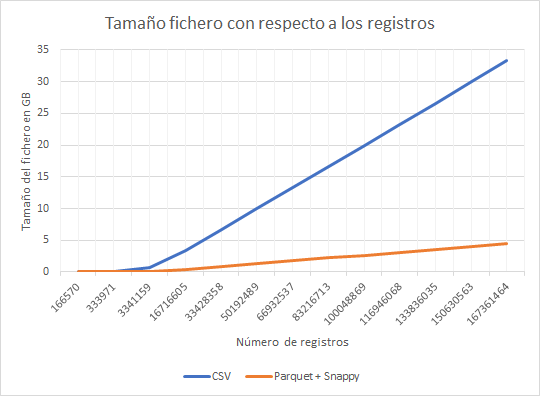
\includegraphics[scale=1]{graficas/espacioFichero}
\end{figure}

\section{Eficiencia de la infraestructura}
Una vez comentados los resultados obtenidos y las pruebas realizadas sobre los ficheros de datos, vamos a proceder a analizar el rendimiento del sistema \textit{big data} con las diferentes configuraciones implementadas. 

Primero comentaremos los resultados obtenidos en el clúster doméstico y, posteriormente, pasaremos a analizar los resultados en el clúster universitario, que son más representativos al tener mayor similitud con un sistema más realista.

En ambos realizaremos todas las pruebas, primero el procesamiento del fichero de datos en los diferentes tamaños (tabla \ref{ficherosCSV}), donde se realizará los cálculos y la limpieza necesaria, y, posteriormente, con los diferentes archivos ya procesados (tabla \ref{ficherosParquet}) realizaremos las cuatro consultas desarrolladas para este trabajo, explicadas en el apartado \ref{impConsultas}.

Para el desarrollo de estas pruebas nos fijaremos en tres aspectos claves para entender el rendimiento del sistema \textit{bigdata}. Estos serán:

\begin{itemize}
	\item \textbf{Tiempo:} Que será el tiempo en realizar la tarea en segundos.
	\item \textbf{Velocidad:} Que será el número de registros procesados por el sistema entre el tiempo en realizar la tarea. $velocidad = \dfrac{nº \; de \; registros \; a \; procesar}{tiempo \; de \; ejecuci\acute{o}n}$
	\item \textbf{Eficiencia:} Que será la velocidad entre el número de núcleos de procesamiento del sistema \textit{big data} \cite{eficiencia}. $eficiencia = \dfrac{velocidad}{nº \; de \; n\acute{u}cleos}$
\end{itemize}

\subsection{Clúster doméstico}
En este apartado, se analizarán y estudiaran los resultados obtenidos por el clúster doméstico tanto en modo pseudo-distribuido, con un solo ordenador, como en el modo multinodo, con un ordenador maestro-esclavo y dos esclavos.

\subsubsection{Procesamiento de datos}
\begin{figure}[htp!]
	\centering
	\caption{Gráfica comparativa del tiempo de procesamiento de los datos por el clúster doméstico}
	\label{gra:tiemProcDom}
	\vspace{5pt}
	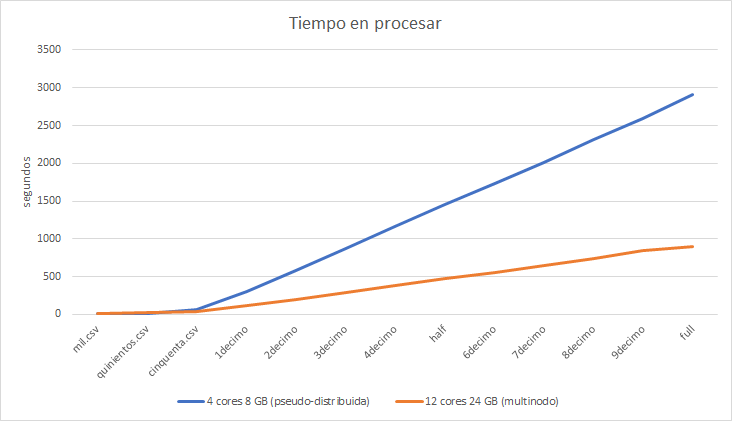
\includegraphics[scale=0.8]{graficas/tpdom}
\end{figure}
\begin{figure}[htp!]
	\centering
	\caption{Gráfica comparativa de la velocidad en el procesamiento de los datos por el clúster doméstico}
	\label{gra:velProcDom}
	\vspace{5pt}
	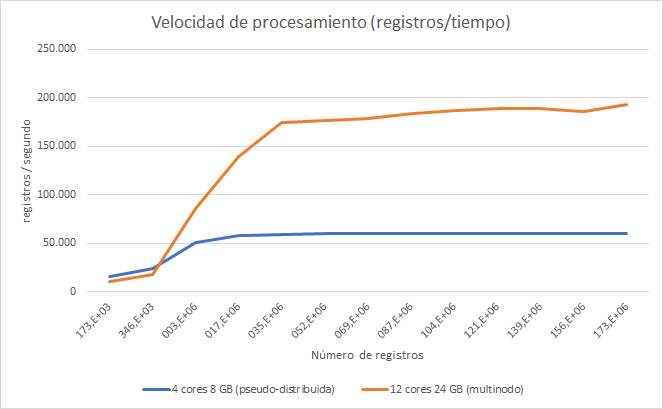
\includegraphics[scale=0.85]{graficas/vpdom}
\end{figure}

En la figura \ref{gra:tiemProcDom} podemos encontrar el tiempo de procesamiento para cada fichero de datos con los que se realizan las pruebas, tanto para el modo pseudo-distribuido (línea azul) como para el modo multinodo (línea naranja). De la misma forma, en la figura \ref{gra:velProcDom} podemos encontrar una gráfica similar pero comparando los registros por segundo que procesa cada configuración.

Ambos resultados resultan acordes con lo esperado, primero, con la propia definición del \textit{big data}, donde estos sistemas no resultan rentables hasta que el volumen de datos es bastante alto. Esto se puede apreciar en ambas gráficas, tanto la de tiempo, como en mayor manera en la de velocidad, donde hasta que no se pasa del millón de registros (a partir del fichero ``cinquenta.csv'') los resultados de ambas configuraciones son muy similares, incluso siendo peor en el caso del multinodo. 

Estos peores resultados en el caso de los ficheros pequeños se puede explicar por el hecho de que el maestro tiene que hacer las distribuciones de los datos entre los tres nodos. Esta transmisión junto con el corto tiempo de ejecución necesario para procesar los mismos hace que la ventaja de añadir capacidad de procesamiento acabe siendo una desventaja al no poder aprovecharse y añadirse al proceso los tiempos de envío de datos.

Sin embargo, es a partir del umbral indicado cuando la velocidad sube en gran manera y se reduce el tiempo de ejecución. Si observamos ambas gráficas, especialmente con el fichero completo, podemos ver que la proporción de tiempo y de registros por segundo es muy similar a la proporción de núcleos de procesamiento de las configuraciones, donde la multinodo tienes tres veces más \gls{CPU}s que la pseudo-distribuida.

Es decir, el tiempo requerido para el procesamiento de la ejecución pseudo-distribuida es casi tres veces mayor que la multinodo. Por otro lado, la cantidad de registros por segundo que procesa la configuración multinodo también es cerca de tres veces mayor. Esto hace pensar que el número de \gls{CPU}s será el factor que influencie los resultados, más que la \gls{RAM}, aunque habrá que confirmarlo con los resultados de las consultas y del clúster universitario.

\begin{figure}[htp!]
	\centering
	\caption{Gráfica comparativa de la eficiencia en el procesamiento de los datos por el clúster doméstico}
	\label{gra:efiProcDom}
	\vspace{5pt}
	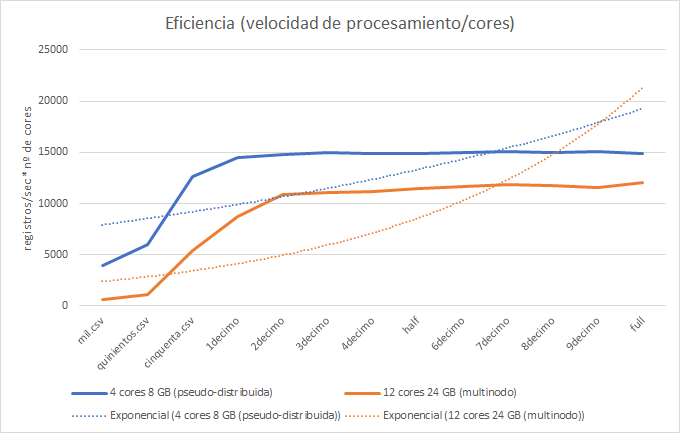
\includegraphics[scale=0.85]{graficas/epdom}
\end{figure}

La figura \ref{gra:efiProcDom} muestra la eficiencia del clúster doméstico en ambas configuraciones. Como se ha explicado anteriormente, la eficiencia es el número de registros que el sistema es capaz de procesar entre el número de \gls{CPU}s de la configuración. En este caso, aparte de apreciar los datos reales, también se ha añadido dos líneas de tendencia para esbozar lo que sucedería si se contase con más datos.

Como apreciamos en la gráfica, vemos como en eficiencia es la configuración pseudo-distribuida la que se muestra por encima en todo momento, queriendo decir que cada núcleo de esta configuración es capaz de procesar más registros por segundo que en el caso de la multinodo. 

Sin embargo, si nos fijamos en la línea de tendencia, vemos como finalmente la configuración multinodo acabaría superando en eficiencia con ficheros con más registros. Este detalle también se puede apreciar con los datos reales, ya que la ejecución pseudo-distribuida se queda estancada a partir del fichero ``2 decimo'' (más de 30 millones de registros) mientras que la multinodo sigue aumentando su eficiencia de forma reducida.

Esto se puede explicar por el proceso de partición de tareas y transmisión de datos, que hace que el sistema tenga que dedicar parte del tiempo de ejecución a establecer las tareas de cada núcleo y a reunir los resultados del procesamiento, haciendo que una configuración donde solo exista un núcleo que tenga que hacer el trabajo sería mejor que otra donde los núcleos se tengan que repartir el trabajo, más si los núcleos están en diferentes computadoras, debido a la latencia de red.

Este efecto solo podría ser contrarrestado, en condiciones normales (donde la partición de tareas y transmisión de datos tomen su tiempo), si la memoria \gls{RAM} dedicada a cada núcleo fuese lo suficientemente grande para albergar todos los datos a procesar y el fichero fuese lo suficientemente grande o si la tarea a realizar necesitase de gran potencia de cálculo.

\subsubsection{Rutas frecuentes}
Para las consultas de rutas frecuentes, como se ha explicado anteriormente (apartado \ref{impConsultas}), existen dos formas de calcularlas. La primera, donde solo se tiene en cuenta la franja de tiempo del día especificado y, otra, donde se da más importancia al día indicado pero también se tienen en cuenta los días iguales cercanos a la fecha introducida, es decir, si se consulta por un viernes, se tienen en cuenta otros viernes cercanos para hacer el cálculo.

\begin{figure}[htp!]
	\centering
	\caption{Gráfica comparativa del tiempo en completar la consulta de rutas frecuentes por el clúster doméstico}
	\label{gra:tiemFreqDom}
	\vspace{5pt}
	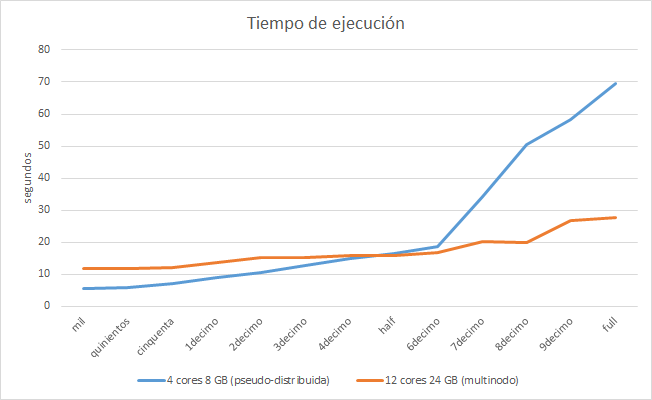
\includegraphics[scale=0.8]{graficas/tfdom}
\end{figure}
\begin{figure}[htp!]
	\centering
	\caption{Gráfica comparativa del tiempo en completar la consulta de rutas frecuentes teniendo en cuenta la estacionalidad por el clúster doméstico}
	\label{gra:tiemFreqDayDom}
	\vspace{5pt}
	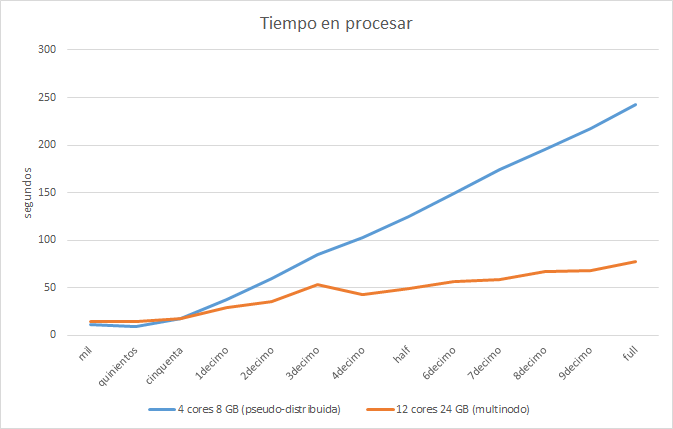
\includegraphics[scale=0.9]{graficas/tfddom}
\end{figure}
\begin{figure}[htp!]
	\centering
	\caption{Gráfica comparativa de la velocidad durante la consulta de rutas frecuentes por el clúster doméstico}
	\label{gra:velFreqDom}
	\vspace{5pt}
	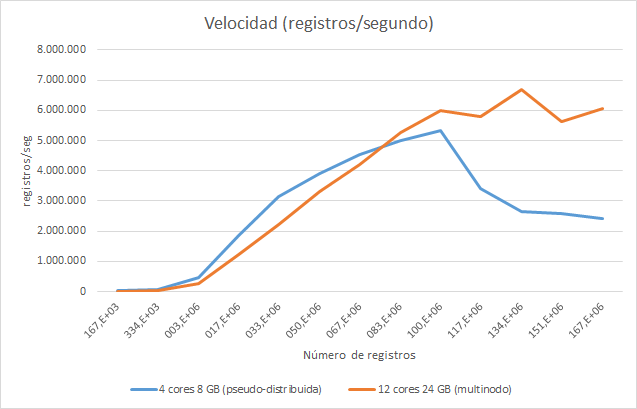
\includegraphics[scale=0.9]{graficas/vfdom}
\end{figure}
\begin{figure}[htp!]
	\centering
	\caption{Gráfica comparativa de la velocidad durante la consulta de rutas frecuentes teniendo en cuenta la estacionalidad por el clúster doméstico}
	\label{gra:velFreqDayDom}
	\vspace{5pt}
	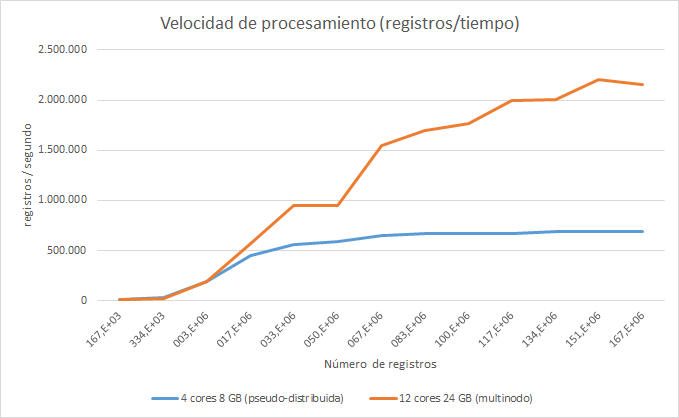
\includegraphics[scale=0.9]{graficas/vfddom}
\end{figure}

La principal diferencia entre estas consultas es el uso de \gls{CPU} necesario, es decir, es la cantidad de cálculos necesarios para obtener los resultados. Aunque ambas realizan un filtrado y una selección, la segunda consulta, al tener en cuenta la estacionalidad, tiene que ponderar las rutas frecuentes de días cercanos, realizando operaciones en como flotante que requieren más cálculos en un ordenador.

Los resultados de tiempo para la primera consulta se pueden apreciar en la figura \ref{gra:tiemFreqDom}, mientras que para la segunda consulta obtenemos los de la figura \ref{gra:tiemFreqDayDom}. Con respecto a la cantidad de registros por segundo de cada consulta, los resultados de la primera se pueden observar en la figura \ref{gra:velFreqDom}, mientras que, los de la segunda están en la figura \ref{gra:velFreqDayDom}.

Si nos paramos a analizar los resultados, la diferencia entre las dos clases es notable, requiriendo bastante menos tiempo la primera consulta, especialmente en el modo pseudo-distribuido. Esto, que arroja una gráfica muy interesante en la figura \ref{gra:tiemFreqDom}, es debido a lo indicado anteriormente sobre los cálculos necesarios para obtener los resultados. En el caso indicado, hasta que no se pasa de los cien millones de registros (fichero ``6decimo'') no es rentable usar una arquitectura \textit{big data} para procesar los datos.

Por otro lado, un aspecto curioso de estas gráficas se encuentra en la figura \ref{gra:velFreqDom} donde la velocidad de la configuración pseudo-distribuida empieza a disminuir a partir de los cien millones de registros en el conjunto de datos, coincidiendo donde empieza a ser rentable el uso de un sistema \textit{big data}. Esta caída del rendimiento es debida a la falta de memoria para almacenar todos los datos en la memoria \gls{RAM} teniendo que acceder al disco para obtener más y, por tanto, produciéndose una ralentización en el proceso. Es aquí donde se puede apreciar de forma clara el efecto de las limitaciones de \gls{RAM}.

Por último, y, en relación a la comparación entre los ficheros \gls{CSV} y los \textit{Parquet} (apartado \ref{compFichDatos}), si comparamos las gráficas de velocidad de estas consultas (figuras \ref{gra:velFreqDom} y \ref{gra:velFreqDayDom}), donde se utiliza \textit{Parquet}, a la de procesamiento de datos (figura \ref{gra:velProcDom}), que lee los \gls{CSV}s originales, se confirma la mayor velocidad de lectura del almacenamiento columnar.

Con respecto a la eficiencia de estas dos consultas, los resultados de la primera se pueden encontrar en la figura \ref{gra:efiFreqDom}, mientras que los de la consulta que tiene en cuenta la estacionalidad se encuentran en la figura \ref{gra:efiFreqDayDom}.

En este caso, para la primera consulta sigue siendo más eficiente el sistema pseudo-distribuido, sin embargo, vemos que para el caso de la segunda consulta esta tendencia cambia a partir del fichero ``8decimo'' que tiene más de 133 millones de registros. Este cambio de tendencia que se produce a partir de este fichero no es debido al tamaño del mismo, si no, como se indicó anteriormente, a la necesidad de cálculo de la consulta para obtener los resultados, que hace que resulte más rentable tener más unidades de procesamiento.

\begin{figure}[htp!]
	\centering
	\caption{Gráfica comparativa de la eficiencia durante la consulta de rutas frecuentes por el clúster doméstico}
	\label{gra:efiFreqDom}
	\vspace{5pt}
	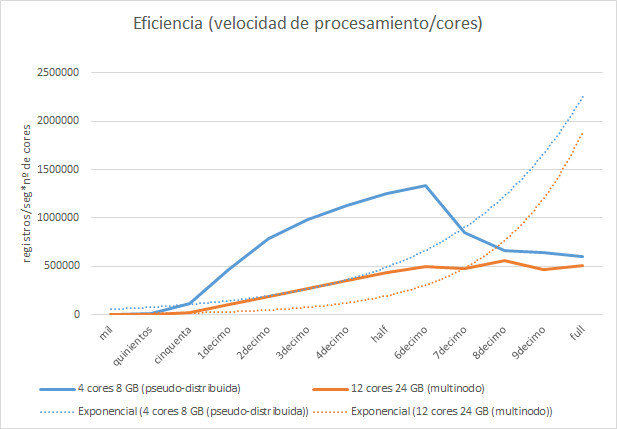
\includegraphics[scale=0.9]{graficas/efdom}
\end{figure}
\begin{figure}[htp!]
	\centering
	\caption{Gráfica comparativa de la eficiencia durante la consulta de rutas frecuentes teniendo en cuenta la estacionalidad por el clúster doméstico}
	\label{gra:efiFreqDayDom}
	\vspace{5pt}
	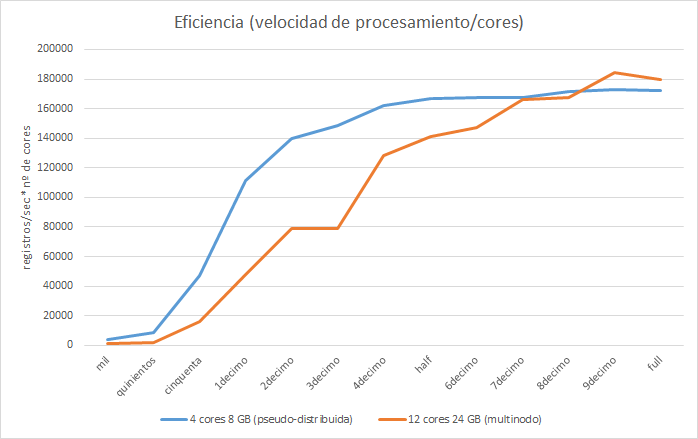
\includegraphics[scale=0.85]{graficas/efddom}
\end{figure}

\subsubsection{Zonas que aportan más beneficios}
Con esta consulta, que calcula las zonas que más beneficios pueden procurarle al taxista a partir de ciertos factores (apartado \ref{profSinExplicacion}), pasa lo mismo que con la consulta de las rutas más frecuentes. Para este trabajo, se han desarrollado dos formas de calcular los datos, la primera teniendo en cuenta solo el día solicitado mientras que, la segunda, tiene en cuenta la estacionalidad.

Estas consultas, que requieren más cálculos que la anterior, acentuará los efectos anteriormente explicados sobre la \gls{CPU}. Además, es este caso, la consulta que tiene en cuenta la estacionalidad es la que más cálculos necesita de las cuatro existentes, representando un ejemplo de uso en un sistema \textit{big data} con gran cantidad de datos e intenso en cálculos.

\begin{figure}[htp!]
	\centering
	\caption{Gráfica comparativa del tiempo en completar la consulta de zonas que reportan más beneficio por el clúster doméstico}
	\label{gra:tiemProDom}
	\vspace{5pt}
	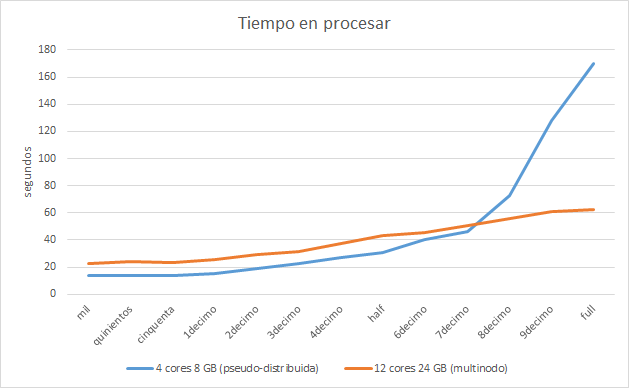
\includegraphics[scale=0.9]{graficas/tbdom}
\end{figure}
\begin{figure}[htp!]
	\centering
	\caption{Gráfica comparativa del tiempo en completar la consulta de zonas que reportan más beneficio teniendo en cuenta la estacionalidad por el clúster doméstico}
	\label{gra:tiemProDayDom}
	\vspace{5pt}
	\includegraphics[scale=0.9]{graficas/tbddom}
\end{figure}
\begin{figure}[htp!]
	\centering
	\caption{Gráfica comparativa de la velocidad durante la consulta de zonas que reportan más beneficio por el clúster doméstico}
	\label{gra:velProDom}
	\vspace{5pt}
	\includegraphics[scale=0.9]{graficas/vbdom}
\end{figure}
\begin{figure}[htp!]
	\centering
	\caption{Gráfica comparativa de la velocidad durante la consulta de zonas que reportan más beneficio teniendo en cuenta la estacionalidad por el clúster doméstico}
	\label{gra:velProDayDom}
	\vspace{5pt}
	\includegraphics[scale=0.9]{graficas/vbddom}
\end{figure}

En la figuras \ref{gra:tiemProDom} y \ref{gra:velProDom} se pueden observar los resultados de tiempo y velocidad de procesamiento de la primera consulta. Por otro lado, en las figuras \ref{gra:tiemProDayDom} y \ref{gra:velProDayDom} se pueden ver las mismas gráficas para la segunda consulta, que tiene en cuenta la estacionalidad.

Como se ha comentado anteriormente, la segunda consulta es la que más tiempo en realizarse requiere, llegando a necesitar más de dos horas en ejecutarse para la configuración pseudo-distribuida, por el poco más de media hora que requiere hacerlo por la multinodo. Es decir, es en este tipo de tareas tan intensas en cálculo y cantidad de datos donde contar con el extra de \gls{CPU} y memoria \gls{RAM} marcan la diferencia.

Si nos fijamos en la figura \ref{gra:velProDayDom}, donde se representa la velocidad de procesamiento de ambas configuraciones, se puede apreciar que la ejecución multinodo es más veloz desde el comienzo de las pruebas, es decir, con el fichero más pequeño, y, la diferencia entre ambas, comienza a ser notable desde los trescientos mil registros. Esto indica el gran número de operaciones que se realizan para calcular los resultados, al contrario que en los resultados anteriores.

Por otro lado, si nos fijamos en las figuras \ref{gra:tiemFreqDom} y \ref{gra:velFreqDom} que son los resultados de tiempo y velocidad de procesamiento de la consulta que no tiene en cuenta la estacionalidad, al igual que en el caso de las rutas frecuentes, vemos que, a partir del archivo ``6decimo'' que tiene cien millones de registros el tiempo empieza a aumentar de forma brusca y la velocidad se reduce en gran manera.

Esto, al igual que lo explicado anteriormente, pone de manifiesto la importancia de contar con la mayor cantidad de \gls{RAM} posible para evitar los accesos a disco, que bajan el rendimiento en gran manera. En este caso la pérdida de velocidad es de un 60\%, haciendo que el rendimiento del sistema se resienta y los tiempos de ejecución aumenten en una media de dos segundo cada diez millones de registros.

Con respecto a la eficiencia, en la figura \ref{gra:efiFreqDom} se pueden observar los resultados para la primera consulta sobre los beneficios de las zonas y, en la figura \ref{gra:efiFreqDayDom} los de la segunda.

Los resultados obtenidos, en el caso de la primera, se mantienen como en la mayoría de consultas anteriores, donde es más eficiente la configuración pseudo-distribuida para todos los ficheros probados aunque la diferencia al final es reducida y se intuye un cambio de tendencia a mayor número de registros en los datos.

Con respecto a la consulta que tiene en cuenta la estacionalidad, como se intuía en las gráficas anteriores y, debido al alto de número de cálculos que realiza y la gran cantidad de datos a procesar, por primera vez, resulta más rentable la configuración multinodo en la mayoría de los archivos probados.

\begin{figure}[htp!]
	\centering
	\caption{Gráfica comparativa de la eficiencia durante la consulta de zonas que reportan más beneficio por el clúster doméstico}
	\label{gra:efiProDom}
	\vspace{5pt}
	\includegraphics[scale=0.85]{graficas/ebdom}
\end{figure}
\begin{figure}[htp!]
	\centering
	\caption{Gráfica comparativa de la eficiencia durante la consulta de zonas que reportan más beneficio teniendo en cuenta la estacionalidad por el clúster doméstico}
	\label{gra:efiProDayDom}
	\vspace{5pt}
	\includegraphics[scale=0.9]{graficas/ebddom}
\end{figure}

\subsection{Clúster universitario}
Tras analizar los resultados del clúster doméstico, en este apartado, se analizarán y estudiaran los resultados obtenidos por el clúster universitario tanto en modo pseudo-distribuido como en el modo multinodo, con las configuraciones indicadas en el apartado \ref{clusterUni}.

Como en el caso anterior, se han realizado las mismas pruebas con los mismos ficheros. La única diferencia es que la prueba de procesamiento de los datos no cuenta con la elaboración de los dos últimos ficheros más grandes, los ficheros ``9decimo'' y ``full'', debido a las limitaciones de cuota de la universidad en los laboratorios.

El punto positivo de este clúster es la homogeneidad de los ordenadores sobre los que se realiza las pruebas, estos, al ser todos iguales, nos permiten realizar pruebas de escalado más precisas, al poder aumentar y reducir las prestaciones del sistema de forma lineal.

En este apartado, las gráficas de eficiencia serán diferentes a las anteriores. Para las realizadas de aquí en adelante se tomaran tres archivos representativos, uno con pocos registros (350.000), otro mediano (51.955.527) y otro más grande (138.548.072), y se comparará la capacidad de procesamiento, en registros por segundo de cada core (velocidad de cada núcleo), para las diferentes configuraciones del multinodo.

Es decir, en el eje $X$ de la gráfica encontraremos el número de cores y, en el eje $Y$, el número de registros por segundo que cada core es capaz de procesar en la configuración. Sin embargo, las gráficas como las del apartado del clúster doméstico estarán situadas en el apéndice \ref{apenEficiencia}. 

\subsubsection{Procesado de datos}
\begin{figure}[htp!]
	\centering
	\caption{Gráfica comparativa del tiempo de procesamiento de los datos por el clúster universitario}
	\label{gra:tiemProcUni}
	\vspace{5pt}
	\includegraphics[scale=0.8]{graficas/tpuni}
\end{figure}
\begin{figure}[htp!]
	\centering
	\caption{Gráfica comparativa de la velocidad en el procesamiento de los datos por el clúster universitario}
	\label{gra:velProcUni}
	\vspace{5pt}
	\includegraphics[scale=0.85]{graficas/vpuni}
\end{figure}

Para el procesamiento de datos, como se ha comentado, no se han podido hacer las pruebas con todos los archivos preparados. En este caso, en la figura \ref{gra:tiemProcUni} podemos encontrar los tiempos de ejecución de las diferentes configuraciones utilizadas y, en la figura \ref{gra:velProcUni}, la velocidad de procesamiento.

Primero, si nos fijamos en los tiempos de procesamiento de las diferentes configuraciones podemos apreciar con claridad el efecto, comentado anteriormente, que produce la transmisión de los datos entre los dispositivos del clúster. Es decir, el cuello de botella que produce la transmisión de las tareas por la red, que hace que los tiempos no se reduzcan proporcionalmente a la potencia.

En este caso, para más de 130 millones de registros, podemos observar que al pasar de la configuración pseudo-distribuida, 4 cores y 8 \gls{GB}, a la primera multinodo, 8 cores y 16 \gls{GB}, el tiempo de la tarea se reduce prácticamente a la mitad, de los 1800 segundos a poco más de 900. En el paso de esta primera configuración a la segunda, 16 cores y 32 GB, también reduce prácticamente a la mitad del tiempo, de 900 segundos a cerca de 500.

Sin embargo, a partir de este momento, la capacidad de procesamiento añadida por el resto de configuraciones no compensa al efecto producido por la comunicación entre los nodos. Especial ejemplo de esto es la diferencia casi nula entre los tiempos de la configuración con 8 y 16 nodos.

Este efecto también se puede apreciar en la figura \ref{gra:velProcUni}, que muestra la velocidad de procesamiento, donde, aunque la capacidad aumenta con cada configuración con más nodo, esta en ningún caso llega al teórico caso de doblar su potencia. 

\begin{figure}[htp!]
	\centering
	\caption{Gráfica comparativa de la eficiencia en el procesamiento de los datos por el clúster universitario}
	\label{gra:efiProcUni}
	\vspace{5pt}
	\includegraphics[scale=0.85]{graficas/epuni2}
\end{figure}

Con respecto a la eficiencia de las diferentes configuraciones, podemos apreciar los resultados en la figura \ref{gra:efiProcUni}, donde se puede comparar la velocidad de cada core para las diferentes configuraciones multinodo. En ella podemos apreciar, de nuevo, que añadir más cores al sistema no implica una mayor capacidad de procesamiento debido al coste de la transmisión de datos.

\subsubsection{Rutas más frecuentes}
\begin{figure}[htp!]
	\centering
	\caption{Gráfica comparativa del tiempo en completar la consulta de rutas frecuentes por el clúster universitario}
	\label{gra:tiemFreqUni}
	\vspace{5pt}
	\includegraphics[scale=0.85]{graficas/tfuni}
\end{figure}
\begin{figure}[htp!]
	\centering
	\caption{Gráfica comparativa del tiempo en completar la consulta de rutas frecuentes teniendo en cuenta la estacionalidad por el clúster universitario}
	\label{gra:tiemFreqDayUni}
	\vspace{5pt}
	\includegraphics[scale=0.85]{graficas/tfduni}
\end{figure}
\begin{figure}[htp!]
	\centering
	\caption{Gráfica comparativa de la velocidad durante la consulta de rutas frecuentes por el clúster universitario}
	\label{gra:velFreqUni}
	\vspace{5pt}
	\includegraphics[scale=0.8]{graficas/vfuni}
\end{figure}
\begin{figure}[htp!]
	\centering
	\caption{Gráfica comparativa de la velocidad durante la consulta de rutas frecuentes teniendo en cuenta la estacionalidad por el clúster universitario}
	\label{gra:velFreqDayUni}
	\vspace{5pt}
	\includegraphics[scale=0.9]{graficas/vfduni}
\end{figure}

Para el clúster universitario, igual que para el doméstico, también se ejecutarán las dos consultas que devuelven la información de las rutas frecuentes. La gráfica con los resultados de tiempos se pueden observar en la figura \ref{gra:tiemFreqUni} para la primera consulta y en la figura \ref{gra:tiemFreqDayUni} para la segunda. Con respecto a la de velocidad de procesamiento, la figura \ref{gra:velFreqUni} para la primera consulta y, para la que tiene en cuenta la estacionalidad, en la figura \ref{gra:velFreqDayUni}.

Si comenzamos analizando la gráfica de tiempos de la primera consulta, figura \ref{gra:tiemFreqUni}, se ve con mayor claridad lo ya explicado anteriormente sobre esta consulta. Al tratarse de un simple filtrado de registros dentro de un franja horaria, para archivos de datos pequeños la configuración pseudo-distribuida es más rápida que cualquiera multinodo, debido al coste de la distribución de las tareas y datos por la red. Sin embargo, vemos como que para archivos mayores esta tendencia cambia y las configuraciones multinodo son el doble de rápidas. Para el archivo ``full'', cerca de 60 segundos para la configuración pseudo-distribuida por los poco más de 20 segundos de la peor multinodo.

La naturaleza de la consulta y el coste de la comunicación entre los nodos es también la culpable de que todas las configuraciones multinodo estén en un rango de 10 segundos [23,34 seg - 16,54 seg] no resultando efectivo añadir más cores al sistema. Esta similitud de procesamiento también se puede apreciar en la figura \ref{gra:velFreqUni}, que muestra como la configuración con dos nodos es superior a la de cuatro en velocidad de procesamiento.

Con respecto a la segunda consulta, cuyos datos se pueden encontrar en las figuras \ref{gra:tiemFreqDayUni} y \ref{gra:velFreqDayUni}, apreciamos que se cumple lo explicado en los resultados del clúster doméstico. Debido a la mayor cantidad de cálculos necesarios por esta, los tiempos de procesamiento son mayores que en la otra consulta y, por ello, la diferencia entre las configuraciones es más notable, produciéndose mejorías cercanas al 50\% hasta las dos últimas, con 8 y 16 nodos, donde la diferencia es de 5 segundos.

\begin{figure}[htp!]
	\centering
	\caption{Gráfica comparativa de la eficiencia durante la consulta de rutas frecuentes por el clúster universitario}
	\label{gra:efiFreqUni}
	\vspace{5pt}
	\includegraphics[scale=0.9]{graficas/efuni2}
\end{figure}
\begin{figure}[htp!]
	\centering
	\caption{Gráfica comparativa de la eficiencia durante la consulta de rutas frecuentes teniendo en cuenta la estacionalidad por el clúster universitario}
	\label{gra:efiFreqDayUni}
	\vspace{5pt}
	\includegraphics[scale=0.9]{graficas/efduni2}
\end{figure}

En cuanto a la eficiencia, en la figura \ref{gra:efiFreqUni} se pueden observar los datos con respecto al número de cores de las configuraciones probadas de la primera consulta. En este caso, lo más interesante de la gráfica se produce para la configuración de dos nodos (ocho cores) para el archivo completo, donde se produce una subida de la eficiencia, en discordancia con lo visto hasta ahora.

Este detalle concuerda con los resultados obtenidos en las figura \ref{gra:tiemFreqUni} y \ref{gra:velFreqUni}, donde se observa que la configuración de 2 nodos es superior a la de 4 en ficheros grandes. Esto puede deberse a que la partición de datos entre los nodos aprovecha de forma optima la memoria \gls{RAM} del sistema y obtiene buenos resultados debido a la minimización que se produce sobre el coste de la comunicación en red.

Con respecto a la segunda consulta, los resultados obtenidos se pueden encontrar en la figura \ref{gra:efiFreqDayUni}, que mantiene lo explicado anteriormente.

\subsubsection{Zonas que aportan más beneficios}
\begin{figure}[htp!]
	\centering
	\caption{Gráfica comparativa del tiempo en completar la consulta de zonas que reportan más beneficio por el clúster universitario}
	\label{gra:tiemProUni}
	\vspace{5pt}
	\includegraphics[scale=0.85]{graficas/tbuni}
\end{figure}
\begin{figure}[htp!]
	\centering
	\caption{Gráfica comparativa del tiempo en completar la consulta de zonas que reportan más beneficio teniendo en cuenta la estacionalidad por el clúster universitario}
	\label{gra:tiemProDayUni}
	\vspace{5pt}
	\includegraphics[scale=0.85]{graficas/tbduni}
\end{figure}
\begin{figure}[htp!]
	\centering
	\caption{Gráfica comparativa de la velocidad durante la consulta de zonas que reportan más beneficio por el clúster universitario}
	\label{gra:velProUni}
	\vspace{5pt}
	\includegraphics[scale=0.85]{graficas/vbuni}
\end{figure}
\begin{figure}[htp!]
	\centering
	\caption{Gráfica comparativa de la velocidad durante la consulta de zonas que reportan más beneficio teniendo en cuenta la estacionalidad por el clúster universitario}
	\label{gra:velProDayUni}
	\vspace{5pt}
	\includegraphics[scale=0.85]{graficas/vbduni}
\end{figure}

En este caso, como con el clúster doméstico, se han ejecutado las dos consultas para obtener las zonas que más beneficio pueden aportar al taxista. Los tiempos de ejecución de la primera, que solo tiene en cuenta la franja horaria deseada, obtiene los tiempos de ejecución que se pueden observar en la figura \ref{gra:tiemProUni}.

Si analizamos estos resultados, vemos que son muy similares a los obtenidos por el clúster doméstico (figura \ref{gra:tiemFreqDom}) donde la diferencia de tiempos entre el modo pseudo-distribuido y el multinodo es casi nula hasta el fichero ``6decimo'' y, tras este, la diferencia se vuelve muy abrupta. Esto también se puede apreciar en la tabla de resultados de la velocidad de procesamiento, figura \ref{gra:velProUni}.

Como se explicó en aquel caso, esto es debido a la falta de memoria \gls{RAM} para almacenar los datos completos, haciendo que sea necesario el acceso a disco y, por tanto, reduciendo la capacidad del sistema. Con respecto a las diferentes configuraciones multinodo, estas mantienen resultados de tiempo y velocidad de procesamiento muy similares, indicando que el uso de \gls{CPU} para cálculo no es suficiente para contrarrestar el coste de la comunicación entre los nodos.

Esto último cambia en el caso de la segunda consulta, donde si se tiene en cuenta la estacionalidad y, por tanto, el número de cálculos necesarios para obtener los resultados es mucho mayor, como se vio en el clúster doméstico. En este caso, los resultados se puede encontrar en la figura \ref{gra:tiemProDayUni} en el caso del tiempo de ejecución y, en la figura \ref{gra:velProDayUni}, para la velocidad de procesamiento.

En este caso, como en el caso del clúster doméstico, es donde se saca el mayor rendimiento a la arquitectura \textit{big data}. Si observamos la tabla \ref{t:tiemfull}, que contiene los tiempos de cada configuración del clúster junto con la diferencia de tiempo con respecto a la configuración anterior en potencia, podemos observar como los tiempos se reducen en más de un 50\% con respecto a su predecesor en potencia.

\begin{table}[htp!]
	\centering
	\caption{Tiempos clúster universitario para archivo ``full'' y diferencia con respecto a la anterior configuración menos potente}
	\label{t:tiemfull}
	\begin{tabular}{|c|c|c|}
		\hline
		\multicolumn{1}{|l|}{}   & \textbf{Tiempo} & \textbf{Diferencia} \\ \hline
		\textbf{4 cores 8 GB}    & 4924,275306     & 100                 \\ \hline
		\textbf{8 cores 16 GB}   & 2566,806429     & 52,1255671          \\ \hline
		\textbf{16 cores 32 GB}  & 1398,539243     & 54,48557504         \\ \hline
		\textbf{32 cores 64 GB}  & 814,9681364     & 58,27281147         \\ \hline
		\textbf{64 cores 128 GB} & 493,53187       & 60,55842529         \\ \hline
	\end{tabular}
\end{table}

Esto resultados representan el funcionamiento ideal de la arquitectura \textit{big data} y se producen debido al alto requerimiento en potencia de cálculo de esta consulta, que realiza varios \textit{joins} de tablas entre los cálculos parciales que efectúa, siendo esta operación muy costosa y consiguiendo contrarrestar, en parte, el coste de la comunicación y envío de los datos por la red.

\begin{figure}[htp!]
	\centering
	\caption{Gráfica comparativa de la eficiencia durante la consulta de zonas que reportan más beneficio por el clúster universitario}
	\label{gra:efiProUni}
	\vspace{5pt}
	\includegraphics[scale=0.85]{graficas/ebuni2}
\end{figure}
\begin{figure}[htp!]
	\centering
	\caption{Gráfica comparativa de la eficiencia durante la consulta de zonas que reportan más beneficio teniendo en cuenta la estacionalidad por el clúster universitario}
	\label{gra:efiProDayUni}
	\vspace{5pt}
	\includegraphics[scale=0.9]{graficas/ebduni2}
\end{figure}

Con respecto a la eficiencia, en el caso de la primera consulta, cuyos resultados se pueden observar en la figura \ref{gra:efiProUni}, son muy similares a lo visto anteriormente, teniendo gran similitud con los resultados obtenidos en la primera consulta de las rutas más frecuentes (figura \ref{gra:efiFreqUni}).

En cuanto a la segunda consulta, cuyos resultados se encuentran en la figura \ref{gra:efiFreqDayUni}, podemos observar como realmente el coste de la transmisión de los datos no es contrarrestado totalmente por la cantidad de cálculos de la consulta, ya que, es más eficiente la configuración pseudo-distribuida en cuanto al procesamiento de registros por segundo en cada core.

Sin embargo, comparado con los resultados obtenidos hasta ahora en cuanto a eficiencia, sí se puede observar el menor grado de la pendiente entre configuraciones con más cores, es decir, la potencia perdida es menor en este caso, debido a la alta cantidad de cálculos que hay que llevar a cabo.

\subsection{Conclusiones sobre el rendimiento}
Tras haber realizado las pruebas en ambos clústeres y analizar los resultados, podemos extraer varias conclusiones. La primera es que hay que tener en cuenta la latencia de red para el diseño del sistema \textit{big data}, ya que, no siempre tener mayor potencia bruta (más núcleos y memoria RAM) implica una mejor respuesta en cuanto a capacidad de procesamiento.

Es decir, hemos visto como, dependiendo de la naturaleza, era hasta negativo añadir más nodos al sistema. Por ello, hay que buscar un equilibrio entre la latencia introducida por la transmisión de los datos en la red y la capacidad de procesamiento añadida de los nodos.

Por otro lado, debido a las decisiones de diseño tomadas en la creación de este sistema \textit{big data}, hemos observado como el número de núcleos resultaba siendo más determinante que la cantidad de memoria \gls{RAM}. Esto se ha debido al mecanismo de compresión utilizado, que, por un lado, requería capacidad de procesamiento para las tareas de descompresión de los ficheros de datos y, por otro, reducía el tamaño de los ficheros de datos, que se podían mantener comprimidos en la memoria \gls{RAM} de los equipos al ser de menor tamaño que sus capacidad total.

Sin embargo, hemos visto como la \gls{RAM} hubiese sido determinante si el tamaño de los datos hubiera sido mayor, ya que en casos como los analizados en la figura \ref{gra:tiemProUni}, en cuanto el sistema se quedaba sin espacio para almacenar los datos y los resultados intermedios en la \gls{RAM}, el rendimiento del sistema se veía fuertemente castigado por los accesos a disco, que son mucho más lentos.

Por tanto, tras expuesto anteriormente, en el proceso de diseño e implementación de un sistema \textit{big data} una de las tareas más importantes es analizar la naturaleza de la tarea que se realizará para poder establecer un equilibrio eficiente entre la capacidad de cómputo de los nodos y la latencia de red. Además, se debe procurar aprovechar al máximo la memoria \gls{RAM} y evitar los accesos a discos, ya sea introduciendo grandes cantidades de \gls{RAM} al sistema o mediante mecanismos de compresión, si la capacidad de cómputo del sistema es suficiente.


%
% Conclusiones
%
\chapter{Conclusiones\label{sec:conclusiones}}

\section{Conclusiones}
El objetivo de este Trabajo de Fin de Grado era el diseño e implementación de una arquitectura \textit{big data} basada en \textit{Apache Spark} que permitiera al usuario la carga, almacenamiento, procesamiento, análisis y la obtención de resultados, sobre unas consultas establecidas, de datos. En esta ocasión, los datos eran el conjunto de todos los viajes de taxi que se realizaron en la ciudad de Nueva York en el año 2013.

Lo que se pretendía con el diseño de la arquitectura es que esta fuese adaptable a las diferentes situaciones en las que se implementaría, también se buscaba que fuese escalable con facilidad y que fuese eficiente, es decir, que hubiese mejoría en los tiempos de procesamiento con las mejoras del sistema \textit{big data}.

Tras la realización del diseño, la implementación y las pruebas de rendimiento sobre esta arquitectura se puede confirmar que se han logrado los objetivos propuestos. Contándose con un sistema \textit{big data} fácilmente adaptable a los diferentes entornos utilizados. También es un sistema escalable, resultando una tarea sencilla la modificación del número de nodos conectados al sistema, y eficiente, logrando resultados en tiempos aceptables para todas las configuraciones y que mejoran con la adición de nodos al mismo.

Además, se ha logrado la implementación de las consultas que se establecieron como objetivo, consiguiendo que el sistema sea capaz de analizar los datos y obtener información útil de los mismos gracias al uso de \textit{Apache Spark}.

Finalmente, la ejecución de las pruebas sobre la arquitectura nos ha permitido confirmar los resultados que se esperaban obtener con las diferentes configuraciones de nodos. Asimismo, estas pruebas nos han permitido conocer los límites y visualizarlos en el conjunto de gráficas, pudiendo conocer las tendencias de comportamiento de las diferentes configuraciones.

\section{Futuras líneas de trabajo}
Existen diversas posibilidades líneas de trabajo para desarrollar este proyecto en el futuro, algunas de estas son:

\begin{itemize}
\item Desarrollo de una herramienta de visualización gráfica de los datos obtenidos por las consultas. Esto llevaría al sistema a estado más cercano para la implementación y uso realista del mismo, al poder permitir a usuarios ajenos entender los datos de una forma sencilla.

\item Creación de una interfaz para el sistema \textit{big data}, que permita la fácil manipulación de la misma, de una forma más amigable para el usuario. Esta línea estaría relacionada con la anterior siendo ambas necesarias para la implantación del sistema.

\item Adaptación del sistema para la aceptación de los datos de otros años \cite{taxiTrips}, de ciudades diferentes, de medios de transporte similares como Uber o Cabify o de datos no relacionados con el transporte como condiciones meteorológicas o eventos en la ciudad. 

\item Adaptación del sistema para la aceptación de datos en tiempo real y uso de algoritmos de inteligencia artificial para predecir los resultados de las consultas y mejorar el conocimiento del taxista.

\item Implementación y despliegue del sistema en servicios en la nube como \gls{AWS} con ajustes de escalabilidad automática en base al uso del sistema.
\end{itemize} 

%
% Planificacion
%
\chapter{Planificación \label{sec:planificación}}
En este apartado se detallará la planificación del proyecto, indicando las diferentes fases del mismo, el desglose de las tareas que las componen y la duración de las mismas.

La planificación para el desarrollo del proyecto establece la duración del mismo en cinco meses, iniciándose este a principios de febrero y finalizando a mediados de junio, para la entrega del mismo y cumplir, así, la fecha de presentación del mismo establecida por la universidad Carlos III de Madrid.

\section{Fases de desarrollo}
En este apartado se describirán las fases en las que se ha dividido el trabajo y el tiempo de dedicado a ellas. Estas serán:

\begin{enumerate}
\item \textbf{Entendimiento del problema e identificación de las necesidades:}
El objetivo de esta fase es el análisis del problema para identificar las necesidades y pasos necesarios para solucionarlo. Se realiza el planteamiento del problema y se deciden las tecnologías a utilizar durante el proyecto y los entornos donde se realizará la implementación.

\begin{itemize}
\item Tiempo de ejecución: 7 días.
\end{itemize}

\clearpage
\item \textbf{Estudio de las tecnologías a utilizar:}
Se estudia el funcionamiento de las tecnologías a utilizar. Se analiza la documentación de \textit{Apache Spark} y se realizan diferentes cursos sobre la tecnología. Durante esta fase se analiza la inclusión de \textit{Apache Hadoop} y \textit{Apache Parquet}, que se acaban aceptando y se realiza su estudio.

\begin{itemize}
\item Tiempo de ejecución: 13 días.
\end{itemize}

\item \textbf{Diseño del sistema:}

Desarrollo teórico de las distintas posibilidades soluciones al problema planteado con las tecnologías establecidas. En esta parte, durante el análisis de las consultas a implementar, se añaden las modificaciones desarrolladas.

\begin{itemize}
\item Tiempo de ejecución: 15 días.
\end{itemize}

\item \textbf{Implementación del sistema en el entorno doméstico:}
Preparación del entorno de implantación y desarrollo del código necesario para desplegar el sistema en el entorno doméstico.
 
\begin{itemize}
\item Tiempo de ejecución: 17 días.
\end{itemize}

\item \textbf{Ejecución de pruebas y evaluación del entorno doméstico:}
En esta fase se produce la realización de la batería de pruebas establecidas para todos los componentes del sistema \textit{big data} en el entorno doméstico para ambas configuraciones. Tras la finalización se comprueban los resultados buscando errores y se repiten las pruebas necesarias.

\begin{itemize}
\item Tiempo de ejecución: 10 días.
\end{itemize}

\item \textbf{Implementación del sistema en el entorno universitario:}
En esta fase se produce el despliegue del sistema \textit{big data} para el entorno universitario. Al ser una adecuación del implementado en el doméstico, la principal tarea es la  del adaptación del sistema a los equipos.

\begin{itemize}
\item Tiempo de ejecución: 5 días.
\end{itemize}

\item \textbf{Ejecución de pruebas y evaluación del entorno universitario:}
En esta fase se produce la realización de la batería de pruebas establecidas para todos los componentes del sistema \textit{big data} en el entorno universitario para ambas configuraciones. Tras la finalización se comprueban los resultados buscando errores y se repiten las pruebas necesarias.

\begin{itemize}
\item Tiempo de ejecución: 7 días.
\end{itemize}

\item \textbf{Análisis de resultados:}
En este proceso se analizan todos los resultados obtenidos de las pruebas, se transforman los datos a un formato cómodo para su manipulación y se realizan las gráficas que se utilizarán en la memoria.

\begin{itemize}
\item Tiempo de ejecución: 9 días.
\end{itemize}

\item \textbf{Elaboración de la memoria:}
Documentación de todo el trabajo realizado en las fases anteriores.

\begin{itemize}
\item Tiempo de ejecución: 15 días.
\end{itemize}
\end{enumerate}

\section{Diagrama de fases de ejecución}
En la figura \ref{fig:ganttdelproyecto} podemos encontrar el diagrama Gantt del proyecto, donde se representan las fases nombradas anteriormente y su duración en el tiempo.

\begin{figure}[htp!]
\centering
\caption{Diagrama Gantt del proyecto}
\label{fig:ganttdelproyecto}
\includegraphics[scale=0.55]{graphics/gantDelProyecto}
\end{figure} 

%
% Presupuesto
%
\chapter{Impacto socioeconómico y presupuesto del proyecto \label{sec:presupuesto}}
En este apartado se va a proceder a realizar un análisis de lo que supondría la aplicación del \textit{big data} en el caso del sector del taxi y, posteriormente, se elaborará el presupuesto del proyecto.

Con respecto al presupuesto, se van a analizar los costes de realización que han supuesto la realización de este Trabajo de Fin de Grado. En este, se tendrán en cuenta los medios empleados durante el desarrollo del proyecto para la elaboración de un presupuesto.

\section{Impacto socieconómico}
Durante este documento se ha comentado en varias ocasiones las bondades del \textit{big data} y el positivo impacto que este produce y producirá en la sociedad. En este apartado, vamos a centrarnos en el tema principal de este proyecto, el estudio de los viajes de los taxis, para analizar el impacto la inclusión de estas tecnologías tendrían en el sector.

En este aspecto, ciudades como Nueva York \cite{taxiTrips} o Estocolmo \cite{impacto1} llevan recogiendo datos de los recorridos de taxis para poder realizar análisis sobre estos datos desde hace varios años.

Los posibles usos de estos datos son muy amplios, yendo desde la mejora del tráfico en las ciudades a la de los beneficios del taxista, como en el caso de la segunda consulta. También existes proyectos más enfocados al usuario, como OpenStreetCab \cite{openstreetcab}, que utiliza los datos abiertos de los servicios de taxis de Nueva York y Londres para ofrecer los proveedores más baratos en la situación deseada.

Por tanto, aunque las aplicaciones \textit{big data} implementadas en la realidad son escasas actualmente, existen proyectos de futuras implementaciones que tendrán un impacto positivo tanto en la calidad del servicio como económicamente para todos los participantes, tanto taxistas como para usuarios o para la administración.

Un aplicación que se está estudiando, es la unión de esta información junto con otros datos abiertos de las ciudades, como la meteorología, la agenda de eventos, el estado de otros métodos de transporte y de las carreteras y ciudades para facilitar a las administraciones el control sobre la ciudad y, así, poder destinar recursos para evitar congestiones.

Por otro lado, la apertura de estos datos, también permite que los individuos interesados puedan hacer estudios sobre los datos donde se obtengan resultados beneficiosos para la sociedad. Un ejemplo de este caso, es el estudio sobre el comportamiento de los taxistas en los aeropuertos de Nueva York \cite{aeropuerto} donde se concluye que es mejor esperar a un nuevo cliente que abandonar el aeropuerto.

Por último, un claro ejemplo de éxito de la aplicación del \textit{big data} lo podemos ver en compañias como Uber \cite{uber} o Lyft, que usan análisis en tiempo real para ajustar los precios de los trayectos. También iniciativas como UberPool que, mediante el procesamiento en tiempo real, es capaz de buscar personas que harán trayectos similares a los que hará el usuario y, así, poder compartir taxi.

\section{Presupuesto del proyecto}
\subsection{Medio empleados}
Los medios empleados en el proyecto serán los siguientes:

\begin{itemize}
\item \textbf{Recursos humanos:} Referidos a las personas que han participado en la elaboración del proyecto.
\begin{itemize}
\item \textbf{1 ingeniero junior:} Adrián Rodríguez Grillo.
\item \textbf{1 ingeniero senior:} Pablo Basanta Val.
\end{itemize}

\item \textbf{Medios materiales:} Referidos a los recursos materiales que se utilizan en durante la elaboración del proyecto.
\begin{itemize}
\item 1 ordenador portátil Acer Aspire V5-572PG.
\item 1 ordenador portátil Acer Aspire E5-575G.
\item 1 ordenador de sobremesa Acer VM661-UQ6600C.
\item 1 memoria \gls{USB} Kingstom 16 GB.
\end{itemize}

\clearpage
\item \textbf{Software y licencias:} Referidos a los programas utilizados durante la elaboración del proyecto, tanto con licencia como de código abierto.
\begin{itemize}
\item 3 Ubuntu 16.10.
\item 1 TeXstudio.
\item 1 Microsoft Office 365 Universitario.
\item 1 Apache Spark 2.1.
\item 1 Apache Hadoop 2.7.3.
\item 1 Visual Studio Code.
\end{itemize}

\item \textbf{Medios inmateriales:}
\begin{itemize}
\item Uso del aula de telemática UC3M (40 horas).
\item Conexión a Internet (5 meses).
\end{itemize}
\end{itemize}

\subsection{Presupuesto del trabajo}
Tras especificar los medios utilizados durante la elaboración del proyecto, en este apartado se realizará el desglose de los gastos para elaborar un presupuesto.

\subsubsection{Recursos humanos}
En la elaboración de este proyecto participan dos personas, con diferente posición en el dentro del mismo, por lo que el salario será diferente para cada caso. Se toman como sueldos brutos los siguientes:

\begin{itemize}
\item \textbf{Sueldo ingeniero junior / hora:} 15 euros.
\item \textbf{Sueldo ingeniero senior / hora:} 30 euros.
\end{itemize}

En la tabla \ref{tab:horasRec} se hace un desglose de las horas de dedicación por tarea de los ingenieros que han trabajado en el proyecto y se calculan las horas totales de cada uno. Tras esto, en la tabla \ref{tab:sueldo}, se calcula el coste del trabajo realizado por cada trabajador y el total de ambos sueldos.

\begin{table}[htp!]
\centering
\caption{Desglose de horas de dedicación de los ingenieros implicados en el proyecto}
\label{tab:horasRec}
\begin{tabular}{|l|r|r|r|}
\hline
\multicolumn{1}{|c|}{\textbf{FASE DEL DESAROLLO}}                                                        & \multicolumn{1}{c|}{\textbf{DIAS}} & \multicolumn{1}{c|}{\textbf{\begin{tabular}[c]{@{}c@{}}HORAS \\ INGENIERO \\ JUNIOR\end{tabular}}} & \multicolumn{1}{c|}{\textbf{\begin{tabular}[c]{@{}c@{}}HORAS \\ INGENIERO \\ SENIOR\end{tabular}}} \\ \hline
\begin{tabular}[c]{@{}l@{}}Entendimiento del problema e\\ identificación de las necesidades\end{tabular} & 7                                  & 30                                                                                                 & 5                                                                                                  \\ \hline
Estudio de las tecnologías a utilizar                                                                    & 13                                 & 100                                                                                                & 2                                                                                                  \\ \hline
Diseño del sistema                                                                                       & 15                                 & 80                                                                                                 & 10                                                                                                 \\ \hline
\begin{tabular}[c]{@{}l@{}}Implementación del sistema \\ en el entorno doméstico\end{tabular}            & 17                                 & 90                                                                                                 & 15                                                                                                 \\ \hline
\begin{tabular}[c]{@{}l@{}}Ejecución de pruebas y evaluación \\ del entorno doméstico\end{tabular}       & 10                                 & 40                                                                                                 & 0                                                                                                  \\ \hline
\begin{tabular}[c]{@{}l@{}}Implementación del sistema \\ en el entorno universitario\end{tabular}        & 5                                  & 20                                                                                                 & 15                                                                                                 \\ \hline
\begin{tabular}[c]{@{}l@{}}Ejecución de pruebas y evaluación \\ del entorno universitario\end{tabular}   & 7                                  & 30                                                                                                 & 5                                                                                                  \\ \hline
Análisis de resultados                                                                                   & 9                                  & 40                                                                                                 & 5                                                                                                  \\ \hline
Elaboración de la memoria                                                                                & 15                                 & 60                                                                                                 & 10                                                                                                 \\ \hline
\multicolumn{1}{|r|}{\textbf{TOTAL}}                                                                     & 98                                 & 490                                                                                                & 67                                                                                                 \\ \hline
\end{tabular}
\end{table}

\begin{table}[htp!]
\centering
\caption{Coste total de los recursos humanos}
\label{tab:sueldo}
\begin{tabular}{|l|l|l|l|l|}
\hline
\multicolumn{1}{|c|}{\textbf{CONCEPTO}} & \multicolumn{1}{c|}{\textbf{CANTIDAD}} & \multicolumn{1}{c|}{\textbf{\begin{tabular}[c]{@{}c@{}}HORAS \\ TRABAJADAS\end{tabular}}} & \multicolumn{1}{c|}{\textbf{\begin{tabular}[c]{@{}c@{}}COSTE POR \\ HORA (€)\end{tabular}}} & \multicolumn{1}{c|}{\textbf{\begin{tabular}[c]{@{}c@{}}COSTE \\ TOTAL (€)\end{tabular}}} \\ \hline
Ingeniero junior                        & 1                                      & 490                                                                                       & 15                                                                                          & 7350                                                                                     \\ \hline
Ingeniero senior                        & 1                                      & 67                                                                                        & 30                                                                                          & 2010                                                                                     \\ \hline
\multicolumn{4}{|r|}{\textbf{TOTAL}}                                                                                                                                                                                                                                       & 9360                                                                                     \\ \hline
\end{tabular}
\end{table}

\clearpage
\subsubsection{Medios materiales}
Para este apartado, los valores de la tasa de depreciación se han obtenido de la página de la Agencia Tributaria Española \cite{depreciacion}.

\begin{table}[htp!]
\centering
\caption{Costes de los medios materiales}
\label{costeMediosMateriales}
\begin{tabular}{|l|l|l|l|l|l|}
\hline
\multicolumn{1}{|c|}{\textbf{CONCEPTO}}                         & \multicolumn{1}{c|}{\textbf{\begin{tabular}[c]{@{}c@{}}CAN-\\ TIDAD\end{tabular}}} & \multicolumn{1}{c|}{\textbf{\begin{tabular}[c]{@{}c@{}}PRECIO \\ (€)\end{tabular}}} & \multicolumn{1}{c|}{\textbf{\begin{tabular}[c]{@{}c@{}}PERIODO \\ DE USO\\ (MESES)\end{tabular}}} & \multicolumn{1}{c|}{\textbf{\begin{tabular}[c]{@{}c@{}}TASA \\ DE \\ DEPRECIACIÓN\end{tabular}}} & \multicolumn{1}{c|}{\textbf{\begin{tabular}[c]{@{}c@{}}COSTE \\ TOTAL \\ (€)\end{tabular}}} \\ \hline
\begin{tabular}[c]{@{}l@{}}Acer Aspire \\ V5-572PG\end{tabular} & 1                                                                                  & 750                                                                                 & 5                                                                                                 & 25,00 \%                                                                                         & 112,5                                                                                       \\ \hline
\begin{tabular}[c]{@{}l@{}}Acer Aspire \\ E5-575G\end{tabular}  & 1                                                                                  & 550                                                                                 & 5                                                                                                 & 25,00 \%                                                                                         & 82,5                                                                                        \\ \hline
\begin{tabular}[c]{@{}l@{}}Acer \\ VM661-UQ6600C\end{tabular}   & 1                                                                                  & 599                                                                                 & 5                                                                                                 & 25,00 \%                                                                                         & 89,85                                                                                       \\ \hline
\begin{tabular}[c]{@{}l@{}}USB Kingstom \\ 16 GB\end{tabular}   & 1                                                                                  & 12                                                                                  & 5                                                                                                 & 30,00 \%                                                                                         & 1,68                                                                                        \\ \hline
\multicolumn{5}{|r|}{\textbf{TOTAL}}                                                                                                                                                                                                                                                                                                                                                                                                              & 286,53                                                                                      \\ \hline
\end{tabular}
\end{table}

\subsubsection{Software y licencias}
Para este apartado, los valores de la tasa de depreciación se han obtenido de la página de la Agencia Tributaria Española \cite{depreciacion}.
\begin{table}[htp!]
\centering
\caption{Coste del software y las licencias}
\label{software}
\begin{tabular}{|l|l|l|l|l|l|}
\hline
\multicolumn{1}{|c|}{\textbf{CONCEPTO}}                                      & \multicolumn{1}{c|}{\textbf{\begin{tabular}[c]{@{}c@{}}CAN-\\ TIDAD\end{tabular}}} & \multicolumn{1}{c|}{\textbf{\begin{tabular}[c]{@{}c@{}}PRECIO\\ (€)\end{tabular}}} & \multicolumn{1}{c|}{\textbf{\begin{tabular}[c]{@{}c@{}}PERIODO \\ DE\\ USO\\ (MESES)\end{tabular}}} & \multicolumn{1}{c|}{\textbf{AMORTIZACIÓN}} & \multicolumn{1}{c|}{\textbf{\begin{tabular}[c]{@{}c@{}}COSTE\\ TOTAL \\ (€)\end{tabular}}} \\ \hline
Ubuntu 16.10                                                                 & 3                                                                                  & 0                                                                                  & 5                                                                                                   & 33,00 \%                                   & 0                                                                                          \\ \hline
TeXstudio                                                                    & 1                                                                                  & 0                                                                                  & 5                                                                                                   & 33,00 \%                                   & 0                                                                                          \\ \hline
\begin{tabular}[c]{@{}l@{}}Microsoft Office\\ 365 Universitario\end{tabular} & 1                                                                                  & 0                                                                                  & 5                                                                                                   & 33,00 \%                                   & 0                                                                                          \\ \hline
\begin{tabular}[c]{@{}l@{}}Apache Spark \\ 2.1\end{tabular}                  & 1                                                                                  & 0                                                                                  & 5                                                                                                   & 33,00 \%                                   & 0                                                                                          \\ \hline
\begin{tabular}[c]{@{}l@{}}Apache Hadoop\\ 2.7.3\end{tabular}                & 1                                                                                  & 0                                                                                  & 5                                                                                                   & 33,00 \%                                   & 0                                                                                          \\ \hline
\begin{tabular}[c]{@{}l@{}}Visual Studio\\ Code\end{tabular}                 & 1                                                                                  & 0                                                                                  & 5                                                                                                   & 33,00 \%                                   & 0                                                                                          \\ \hline
\multicolumn{5}{|r|}{\textbf{TOTAL}}                                                                                                                                                                                                                                                                                                                                                                      & 0                                                                                          \\ \hline
\end{tabular}
\end{table}

\clearpage
\subsubsection{Medios inmateriales}
\begin{table}[htp!]
\centering
\caption{Costes de los medios inmateriales}
\label{inmateriales}
\begin{tabular}{|l|l|l|l|l|}
\hline
\multicolumn{1}{|c|}{\textbf{CONCEPTO}} & \multicolumn{1}{c|}{\textbf{CANTIDAD}} & \multicolumn{1}{c|}{\textbf{\begin{tabular}[c]{@{}c@{}}TIEMPO \\ DE\\ USO\end{tabular}}} & \multicolumn{1}{c|}{\textbf{\begin{tabular}[c]{@{}c@{}}COSTE\\ (€)\end{tabular}}} & \multicolumn{1}{c|}{\textbf{\begin{tabular}[c]{@{}c@{}}COSTE\\ TOTAL\\ (€)\end{tabular}}} \\ \hline
Aula telemática                         & 1                                      & 40 horas                                                                                 & 0                                                                                 & 0                                                                                         \\ \hline
Conexión a Internet                     & 1                                      & 5 meses                                                                                  & 45 €/mes                                                                          & 225                                                                                       \\ \hline
\multicolumn{4}{|r|}{\textbf{TOTAL}}                                                                                                                                                                                                                            & 225                                                                                       \\ \hline
\end{tabular}
\end{table}

\subsubsection{Coste total}
\begin{table}[htp!]
\centering
\caption{Coste total del proyecto}
\label{costeTotal}
\begin{tabular}{|l|l|}
\hline
\multicolumn{1}{|c|}{\textbf{CONCEPTO}} & \multicolumn{1}{c|}{\textbf{COSTE (€)}} \\ \hline
Recursos humanos                        & 9360                                    \\ \hline
Medios materiales                       & 286,53                                  \\ \hline
Software y licencias                    & 0                                       \\ \hline
Otros medios                            & 225                                     \\ \hline
\multicolumn{1}{|r|}{\textbf{TOTAL}}    & 9871,53                                 \\ \hline
\end{tabular}
\end{table}

El coste total del proyecto será la suma de los gastos de diferentes tipos de medios. Este coste quedará fijado en 9871.53€ (Nueve mil ochocientos setenta y un euros con cincuenta y tres céntimos) y este se puede encontrar en la table \ref{costeTotal}. 

%
% Presupuesto
%
\chapter{Extended abstract \label{sec:resumenIngles}}

Because of the digital transformation process that is happening nowadays in the society, specially, in the business world, data generation and traffic has grown very abruptly. Every day, millions of Terabytes of new data are generated \cite{BDStats}.

The origin of this data is very varied but the main reason of this exponential growth is the irruption of the connected devices in the daily life of the people. Specifically, the increase in the numbers of the smartphones in use \cite{phoneGrowth} and, more recently, the apparition of the Internet of the Things (IOT) and the wearables, are the main drivers in this growth of the quantity of data generated.

This great volume of data makes the processing task a very costly operation in perspective with the past. Moreover, the use of different sources makes the data structure heterogeneous, increasing the complexity of the processing job. This two issues has made necessary the development of new tools that achieve this task, known as \textit{big data}.

The objective that business and organizations has with the use of this technology is to get valuable information for them that help to structure their market strategy and take some advantage from their competitors. But there are also organizations and public actors that are using these tools to improve the efficiency of some systems. Real time analysis is gaining special relevance nowadays for this optimizing task, for example in traffic systems.

In this Final Degree Project, we are going to take as starting point the challenge gave during the 2015 \gls{DEBS} Grand Challenge. We are going to work with all the traces of the trips made during 2013 by the New York City taxis, which were more than 170 million of trips, and we will do some queries in them, measuring the efficiency of the systems used. There will be two queries, one that search the top ten frequent routes and the top ten profitable areas for the taxi driver, both of them taking in consideration a time window to do it.

In this document we will present the designs of the \textit{big data} architecture implemented. This architecture will be based and developed in \textit{Apache Spark} \cite{spark} in all of its implementations and the distributed file system of \textit{Apache Hadoop} \cite{hadoop} in some. \textit{Apache Parquet} \cite{parquet} will be used for the files to save the processed data as a file type.

To obtain the required results, the user will have to interact with the \textit{big data} system. The first step, after getting the data, will be loading the data. This data will be processed by the system to accommodate the data to the requirements of the challenge. The last step will be the data analysis of the processed data to obtain the results of the queries.

\section{Objetives}
The main objective of this project is the design and implementation of a scalable and efficient \textit{big data} system that address the queries proposed in the \gls{DEBS} Grand Challenge of 2015. To achieve this goal, the project will have the next work phases:

\begin{itemize}
\item Analysis and study of \textit{big data} paradigm and tools available nowadays.

\item Study of the problem to solve, both the data given and the questions to solve.
	
\item Design of the \textit{big data} architecture for the different configurations and situations that are going to be tested.
	
\item Implementation of the different versions of the \textit{big data} architecture designed for the environments that will be tested.
	
\item Design and implementation of the classes and scripts that are going to be responsible of the data processing and the execution of the queries.
	
\item Execution of the scripts developed to make the test and obtain the results both the data and the execution time and system efficiency.
	
\item Analysis of the results, comparing the designs tested in varied environments and configurations.
	
\item Starting off the analysis of the results, conclusions and future lines of work.
\end{itemize}

\section{State of the art}
In this section, the context and the state of the technologies that will be used in this project will be analysed. To do so, we are going to describe the actual situation of open data, \textit{big data} and the tools Apache Spark, Hadoop and Parquet.

\subsection{Open Data} 
In this project, we are going to use the traces of all the trips done in 2013 by all the yellow cabs of New York city. This data is available because of a \Gls{FOIL} petition that Chris Whong made. Nowadays, this tendency is changing and more data is being uploaded for free by organizations and governmental organisms.

This kind of data is called open data, it is information that is available for everyone without any kind of limitations like copyright, patents or other type of control mechanism. This data could be used and distributed with total freedom by anyone \cite{opendata}.

This movement that is being held for a great number of governmental and no-governmental organisms \cite{onudata} \cite{datosMadrid} has some good consequences. There are estimations that say that more than 3 billion of dollars could be generated because of the data opening process \cite{revenueOpenData}. In Europe case, it is estimated that more than 1.7 billion of Euros will be saved by the public administration with this movement.

\subsection{Big data}
\textit{Big data} is defined as a paradigm for enabling the collection, storage, management, analysis and visualization, potentially under real-time constraints, of extensive datasets with heterogeneous characteristics \cite{estandar}. This definition has been made by an agency of the UN dedicated to the study of the technologies of the information.

Another thing that defines this paradigm is the \textit{big data} V’s that have changing in number during the last years \cite{ayuso} \cite{4v} \cite{monse} \cite{soriano}, but there are four V’s that fit perfectly for this definition and are the following:

\begin{itemize}
\item \textbf{Volume:} Referred to data size and quantity. There is not any limit stablished but these quantities grow every day.
\item \textbf{Velocity:} Referred to the speed to access to data, a real-time analysis is the objective stablished.
\item \textbf{Variety:} Referred to the number of different sources of data used. \textit{Big data} systems need to be able to process data with diverse origins and structures.
\item \textbf{Veracity:} Referred to the certainty that the data in the system have are reliable. \textit{Big data} systems should attempt to exclude all the false information to not loose efficiency. 
\end{itemize}

\textit{Big data} is being used by a lot of big enterprises and business, but the success of their use is making that everyone is trying to use it, being a growing market nowadays. Organizations use these systems to extract valuable information of all their data with the objective of get some advantage over their opponent.

\textit{Big data} is also a growing market with growing estimations between 4\% and 15\% per year, generating more than 18 billion dollars in 2014 and with an estimation of being more than 92 billion dollars in 2020 \cite{forecast}. One kind of business that is taking strength is the \gls{BDaaS}, companies that offer to other companies an specialised big data service to analyse their data. 

\subsection{Distributed systems}
Distributed computation is a model of computation where there are some computers that are connected, but they do not share their physical location, with the end of sharing the task and complete them in less time. So, it is a network of autonomous computers that talk between them to achieve an objective, this kind of systems are called clusters \cite{computacionDistribuidad}.

This model of computation offers some advantages like shared resources, scalability, fault-tolerance, concurrence and variety of hardware and software. But it also have some disadvantages like the complexity of the systems, the possibility of have security problems and disparity in the behaviour and the results obtained depending of the situation.

\begin{figure}[htp!]
	\centering
	\caption{Distributed computation scheme \cite{fotodistribuida}}
	\label{distribuidaEng}
	\vspace{5pt}
	\includegraphics[scale=0.3]{graphics/computaciondistribuida}
\end{figure}

There are two main type of configurations on this system, the client-server, where there is a node which offers all the contents to other computers (the clients) which connect to the first one. This mode is used in the World Wide Web, but it has important problems, one produced when the server goes off, that the contents become unreachable and, other, when the server has a lot of connections stablished, because the performance is reduced.

The other mode is the peer-to-peer where all the computers of the network share the work between them and all the machines contribute with their memory and computation power. There is a variation of this configuration where there is a machine that control the network and the rest are the ones that make the work, this relation is called master-slave and it is the one which is going to be used in this project.

\subsection{Apache Spark}
\textit{Apache Spark} \cite{spark} is an open-source \gls{framework} that allows distributed data computation. It is developed in Scala \cite{scala}, but has support for Java, Python and R and it offers an \gls{API} to create distributed systems and deploy them to process data.

This \gls{API} is based in a data structure called Resilient Distributed Dataset (\gls{RDD}) where the data is stored, it has some qualities like its immutability, partitioning capacity and changes history that allows its parallel modification and to recover from failures. The framework uses the \gls{RAM} memory to store the data, being very quick the access to it. That makes \textit{Apache Spark} very good doing iterative jobs with the data.

\begin{figure}[htp!]
	\centering
	\caption{\textit{Apache Spark} components \cite{partsSpark}}
	\label{partSparkEng}
	\vspace{5pt}
	\includegraphics[scale=0.31]{graphics/partSpark}
\end{figure}

Other advantages of using \textit{Apache Spark} is its capacity to use most of file types to storage data and its integration with storage systems that facilitates the task of introducing data in the system. The framework also has some built-in libraries to do different task, these are:

\begin{itemize}
\item \textbf{Spark SQL:} That allows the use of structured and semi-structured data and the use of the SQL language to modify it.
\item \textbf{Spark Streaming:} That allows the analysis of real-time data with use of mini-batches generated with this data.
\item \textbf{MLib:} It is a machine learning library that allows the system to do different kind of analysis like clustering, classifications, regressions, etc.
\item \textbf{GraphX:} Allows parallel graph computation. Because of the immutability of the \gls{RDD}s it is not suitable for graphs that get updates.
\end{itemize}

\subsection{Apache Hadoop}
\textit{Apache Hadoop} \cite{hadoop} is another open-source \gls{framework} which enables the treatment of large datasets in a distributed way. Developed in Java it is used to manage distributed systems, being the fault-tolerance one of its most important qualities. 

It has four main modules, the Hadoop Common which supports the rest of them, the Hadoop Distributed File System (\gls{HDFS}) which is a distributed file system, Hadoop YARN which is a framework to manage the works of the nodes and Hadoop Mapreduce, based in YARN, it is used for parallel processing. In this project only the HDFS will be used, to replicate the data in the distributed configuration in the domestic cluster.

\gls{HDFS} is a distributed file system that gives to the system some important qualities in like replication of the data in the different nodes, fault-tolerance support and a way to save very large files. It uses a master-slave architecture.

\begin{figure}[htp!]
	\centering
	\caption{\gls{HDFS} architecture \cite{hadoop}}
	\label{hdfsarchitectureEng}
	\vspace{5pt}
	\includegraphics[scale=0.6]{graphics/hdfsarchitecture}
\end{figure}

\subsection{Apache Parquet}
\textit{Apache Parquet} \cite{parquet} is an open-source column-oriented file type of the Hadoop ecosystem, compatible with \textit{Apache Hadoop} and \textit{Spark}. It provides an efficient model of storage with an effective compression and codification system.

The columnar storage way saves the data table in columns rather than in rows being faster to access the data as it is not necessary to discard attributes to get the desired one. It is also better to store the data, especially in the case when the values repeat in some records.

In this project \textit{Snappy} \cite{snappyLib} will be used as the library to compress the data files, it fits very well because of the native support of the file type. This library doesn’t seek for the minimum file size, its best quality is its compression and extraction speed.

\begin{figure}[htp!]
	\centering
	\caption{Row and columnar storage models \cite{column}}
	\label{columnEng}
	\vspace{5pt}
	\includegraphics[scale=0.7]{graphics/column}
\end{figure}

\section{Design}
As it have been said, the goal of this project is the design and the implementation of a \textit{big data} architecture to process the traces of the taxi trips in New York city. Also, as another objective is to detect the limitations of the system in different environments, the implementation will be done in domestic and university ones that will make that the design suffers from some modifications depending of the execution environment.

The system will count with an only role, the administrator, that will be capable of doing all the task that the architecture will do, which are the load of the data, the process task of the data, the execution of the queries and the access to the results. For doing so, the system will count with three modules, described below:

\begin{itemize}
\item \textbf{Data loading and storage:} This module will take care of the data available in the system, will allow the user to upload the original traces of the challenge and, also, will be on charge of the data generated by the other modules.
\item \textbf{Data processing:} This module will be in charge of the data cleaning, eliminating the records with bad information, and of the data transformation, some attributes will change to adapt to the challenge rules.
\item \textbf{Query execution:} This module will provide the results to the problem through the execution of the queries exposed in the challenge.
\end{itemize}

These modules will interact among them and with the user to provide all the functionality of the system. 

On the other hand, as to the architecture of the system as it was said it will be implemented in two environments, the domestic and the university ones, and it also will allow two modes of execution, the pseudo-distributed where only one computer will be used and the distributed one, where there will be some machines.

As it was said, the pseudo-distributed system will count only with one computer. Thus, the jobs will be shared between the cores of the \gls{CPU}, one process will be the master of the rest and they will use de \gls{CPU} as needed. This kind of system have some advantages as they are easy to implement and to maintain but, on the other hand, it computational capacity is low compared with the distributed configuration.

\begin{figure}[htp!]
	\centering
	\caption{\textit{Apache Spark} distributed mode \cite{clusterfoto}}
	\label{fig:clusterSparkEN}
	\includegraphics[scale=0.6]{graphics/sparkCluster}
\end{figure} 

In the figure \ref{fig:clusterSparkEN} we can find the structure of a distributed system mounted with \textit{Apache Spark}, this will be the aspect of the multimode configuration on our system. As we can see, the master node will contain the \textit{SparkContext} job and will control the rest of the nodes.

This distributed system will count with two different implementations as two different environments will be used, these two designs will be:

\begin{itemize}
\item \textbf{Domestic cluster:} Will count with two laptops and one tower pc so the limit here will be the specs of the system, as the computers are low-tier ones. The main difference with the other cluster is the use of \gls{HDFS} to replicate the data between the computers, to eliminate big quantity data sending during the execution of the job. Figure \ref{domEN}
 
\item \textbf{University cluster:} In this case, the system count with a \gls{NFS} so the data is accessible by all the nodes of the architecture without doing any extra effort. This design is very similar to the pseudo-distributed one but using more machines. In this case, two, four, eight and sixteen nodes will be used. Figure \ref{uniEN}.
\end{itemize}

\begin{figure}[htp!]
\centering
\caption{Domestic cluster architecture}
\label{domEN}
\includegraphics[scale=0.3]{graphics/DomENG}
\end{figure}

\begin{figure}[htp!]
\centering
\caption{University cluster architecture}
\label{uniEN}
\includegraphics[scale=0.25]{graphics/uniEN}
\end{figure}

\section{Implementation}
Three different configurations of the architecture will be implemented and tested in the two different environments commented. Although the core of the system will be the same for the three configurations, they will be based in \textit{Apache Spark}, the module of data processing and queries will be the same and they will be use \textit{Apache Parquet} as file type to save the data. These three configurations will be:

\begin{itemize}
\item Pseudo-distributed: This configuration will be tested in both environments and it has the easier configuration as it formed by one computer.
\item Domestic cluster: This configuration will be tested in the domestic environment with the configuration explained in the figure \ref{domEN}. It will use \textit{Apache Hadoop} as a data replication system is needed to make the data available in the slaves.
\item University cluster: This configuration will be tested in the university environment with the configuration explained in the figure \ref{uniEN}. It will use the \gls{NFS} available in the laboratory, so the data will be in each node without the necessity of a replication system.
\end{itemize}

To deploy the \textit{big data} system some steps will be needed before its implementation, this steps are the installation of Linux in the machines that will be used, the installation of Java, Scala, Python and \gls{SSH}, \textit{Apache Spark} and \textit{Apache Hadoop} (where is needed) in every machine utilised during this project. It is also required the configuration of the operating system, to stablish user groups and paths to avoid permission and execution problems, and the configuration of the technologies used to create the connections among the machines.

After this first steps, the implementation will require some steps to get a working system:

\begin{enumerate}
\item Obtaining the data.
\item Data loading.
\item Data analysis and processing.
\item Queries implementation.
\end{enumerate}

\subsection{Obtaining the data}
The file with all the taxi trips of Ney York city during 2013 is a 33 \gls{GB} \gls{CSV} file that can be downloaded from the webpage of the competition \cite{G
grandChallenge}. This file is called ``sorted\_data\_full.csv’’ and will be the base file for all the future work. It will be renamed to ```full.csv’’ and twelve more data files will be created from parts of its data, following the table \ref{ficherosCSV}.

\subsection{Data loading}
In this part, the data generated in the last step will be loaded in to the system to make it available for all the nodes of the system. In the case of the domestic cluster the data will be loaded through the command write in the code fragment \ref{cargaFicheroHDFS}

\subsection{Data analysis and processing}
In this step, after the analysis of the traces of the trip, the component in charge of cleaning and process the data will be developed. For the cleaning process, this module will remove from the data the records that have any kind of attribute with a wrong value, for example values with 0, and it also will check that the coordinates correspond with the city of New York, deleting the records that start or finish out of the city.

In the case of the processing task, the module will transform the data in different ways. First, for the correct implementation of the queries, the coordinates will be transformed to a grid with cells \ref{cuadricula}. Moreover, a new attribute with the day of the week of the trip will be added to facilitate filtering. Secondly, some attributes with no use in the queries will be deleted saving disk space.

\subsection{Implementation of the queries}
The challenge asked for two queries over the data given, but for this project, the final number of queries implemented is four because a modification over the original queries have been made to take seasonality of the data in mind, increasing the computational needs. 

These modifications have been made to test the capacity of the system when a lot of operations are needed to obtain the results, as an influence factor have been added to calculate the influence of the trips depending of the date. In summary, these modifications take in consideration all the trips of the data file and make float operations to calculate the influence in the final results, needing more resources to be executed than the originals, which limit the data to a time window.

The queries implemented had been:

\begin{itemize}
\item \textbf{Frequent routes:} This query return the top 10 most frequent routes during the last 30 minutes. 
\item \textbf{Frequent routes with seasonality:} This query return the top 10 most frequent routes taking in mind a time window of thirty minutes and the day of the week. This query search in all the trips that adjust to these attributes and calculate its influence depending of the difference of dates.
\item \textbf{Profitable areas:} This query return the top ten areas that are currently most profitable for taxi drivers. The profitability of a zone its calculated with the price paid for the trips started in the zona during the last 15 minutes divided for the number of free taxis in the zone.
\item \textbf{Profitable areas with seasonality:} This query return the top ten areas that are currently most profitable for taxi drivers. As the other query with seasonality it takes in consideration all the trips made during the day of the week and the time window stablished.
\end{itemize}

\section{Results}
In this section, we will analyse the results obtained after making the test to the different configurations of the system and environments. This test will focus in two factors, first, the number of nodes of the system, comparing the results of the different numbers. Secondly, the size of the dataset, comparing the results using different sizes of the file with the trips.

\subsection{Test environments}
As it has been said, there will be two main modes of execution in the system, the pseudo-distributed and the distributed, and, also, there are two environments, the domestic and the university one.

The pseudo-distributed mode will we tried in every environment and will be used as guide to comparing the time with the distributed time. In the case of the distributed mode, there are different implementations for each environment. The university cluster will count with more test as the number of nodes will change to compare the scalability of the architecture.

The pseudo-distributed configuration will count with the computer of the table \ref{maestroDomestico} whereas in the university will be the computer of the table \ref{equipoUniversitario}. In the case of the distributed configuration, in the domestic cluster the master will be the computer of the table \ref{maestroDomestico} and the slaves will be the ones on the tables \ref{esclavo1} and \ref{esclavo2}. In the university lab all the machines are the same, the one of the table \ref{equipoUniversitario}.

\subsection{Data files}
As it was commented during the implementation phase, the system will use \textit{Apache Parquet} to save the clean and processed data. The decision was taken because this file type had better read speeds and because of its compression system, that allow us to compress the 33 \gls{GB} file to another of less than 5 GB.

The speed and size comparison could be seen in the tables \ref{velocidadCSVEN} and \ref{velocidadParquetEN}.

\begin{table}[htp!]
	\centering
	\caption{Files and read test for \gls{CSV}}
	\label{velocidadCSVEN}
	\begin{tabular}{|l|l|l|l|l|}
		\hline
		\multicolumn{5}{|c|}{\textbf{CSV}}                                                                               \\ \hline
		\textbf{Filename} & \textbf{Records} & \textbf{Size (GB)} & \textbf{Time (seg)} & \textbf{Records/seg} \\ \hline
		mil.csv         & 173185             & 0,032519531     & 0,99720043                 & 173671                     \\ \hline
		quinientos.csv  & 346370             & 0,065039063     & 1,959946904                & 176724                     \\ \hline
		cinquenta.csv   & 3463702            & 0,649707031     & 15,24788392                & 227159                     \\ \hline
		1decimo.csv     & 17318509           & 3,3             & 494,5507809                & 35018                      \\ \hline
		2decimo.csv     & 34637018           & 6,7             & 389,0821234                & 89022                      \\ \hline
		3decimo.csv     & 51955527           & 10              & 291,1400167                & 178455                     \\ \hline
		4decimo.csv     & 69274036           & 13,3            & 182,5482055                & 379483                     \\ \hline
		half.csv        & 86592546           & 16,6            & 86,86696803                & 996840                     \\ \hline
		6decimo.csv     & 103911055          & 20              & 585,2277942                & 177556                     \\ \hline
		7decimo.csv     & 121229563          & 23,3            & 703,9244393                & 172219                     \\ \hline
		8decimo.csv     & 138548072          & 26,6            & 827,5500103                & 167419                     \\ \hline
		9decimo.csv     & 155866581          & 30              & 952,5683697                & 163627                     \\ \hline
		full.csv        & 173185091          & 33,3            & 978,0770412                & 177066                     \\ \hline
		&                    &                      & \textbf{Tiempo total (seg)} & \textbf{Media reg/seg}     \\ \hline
		&                    &                 & 5509,740781                & 239558,3846                \\ \hline
	\end{tabular}
\end{table}

\begin{table}[htp!]
	\centering
	\caption{Files and read test for \textit{Parquet}}
	\label{velocidadParquetEN}
	\begin{tabular}{|l|l|l|l|l|}
		\hline
		\multicolumn{5}{|c|}{\textbf{PARQUET + SNAPPY}}                                                                          \\ \hline
		\textbf{Filename} & \textbf{Records} & \textbf{Size (GB)} & \textbf{Time (seg)} & \textbf{Records/seg} \\ \hline
		mil.parquet        & 166570             & 0,0078125            & 0,088930148                 & 1873043                    \\ \hline
		quinientos.parquet & 333971             & 0,012304688          & 0,10375922                  & 3218711                    \\ \hline
		cinquenta.parquet  & 3341159            & 0,089160156          & 0,13233389                  & 25247946                   \\ \hline
		1decimo.parquet    & 16716605           & 0,44140625           & 0,533758281                 & 31318680                   \\ \hline
		2decimo.parquet    & 33428358           & 0,883789063          & 1,172321222                 & 28514674                   \\ \hline
		3decimo.parquet    & 50192489           & 1,32                 & 1,802668324                 & 27843440                   \\ \hline
		4decimo.parquet    & 66932537           & 1,76                 & 2,563482635                 & 26110002                   \\ \hline
		half.parquet       & 83216713           & 2,2                  & 3,21071474                  & 25918438                   \\ \hline
		6decimo.parquet    & 100048869          & 2,65                 & 3,437491023                 & 29105201                   \\ \hline
		7decimo.parquet    & 116946068          & 3,11                 & 6,598058132                 & 17724316                   \\ \hline
		8decimo.parquet    & 133836035          & 3,56                 & 10,72142728                 & 12483042                   \\ \hline
		9decimo.parquet    & 150630563          & 4,01                 & 8,413226073                 & 17904019                   \\ \hline
		full.parquet       & 167361464          & 4,46                 & 19,46584598                 & 8597697                    \\ \hline
		                   &                    &                      & \textbf{Tiempo total (seg)} & \textbf{Media reg/seg}     \\ \hline
						   &                    &                      & 58,24401784                 & 19681477,62                \\ \hline
	\end{tabular}
\end{table}

\subsection{Architecture performance}
In this chapter, the results obtained with the different configurations of the system will be analysed, first, the ones obtained in the domestic environment and then, the ones obtained in the university environment, which represents better a real situation as all the machines has the same specs.

The test made measure three aspects of the systems, related among them, but necessary to understand the performance. This three aspects are:

\begin{itemize}
	\item \textbf{Time:} Elapsed time to complete the task in seconds.
	\item \textbf{Speed:} Quantity of records processed per second during the realisation of the task $speed = \dfrac{nº \; of \; records}{execution \; time}$
	\item \textbf{Efficiency:} Speed divide by the system cores. \cite{eficiencia}. $efficiency = \dfrac{speed}{nº \; of \; cores}$
\end{itemize}

The obtained results could be seen in the following graphs. If we look to the results, the first thing that one notice is that the distributed configurations are less time efficient than the pseudo-distributed one until the size of the file is big enough. This is one of the premises of \textit{big data}. This problem is bigger in the queries that don’t require a lot of computation, because the threshold is higher in these cases. This is caused because of the time lost in the distribution of the task between the nodes.

Other visible aspect, especially in the university cluster where the configurations follow a linear incrementation of the resources, is that the time required for finishing the task is inversely proportional to the increase in specs of the cluster. In other words, if the specs of one configuration is the double to the specs of other, the execution time will be nearly the half of the time.

This aspect, although it is true for configurations with low number of nodes, for example, going from two to four nodes, in the case of big numbers it is not always true, for example, from eight to sixteen nodes. This is caused because at that levels the specs increase provided do not worth the latency time between the nodes.

Thus, a balance between the number of nodes and the latency between them should be seek for the most efficient system. Another conclusion that we can extract from the results obtained is that in this architecture the number of cores in the system were more determining than the \gls{RAM}. This was caused because of the compression of the data, as we have the data compressed the \gls{CPU} were more necessary to get access the data. 

Nevertheless, it could be seen how having limited memory affects to the system, loosing efficiency as disk accesses were necessary, which is a slower operation compared with the access to \gls{RAM} memory.


\subsubsection{Domestic cluster}
\begin{figure}[htp!]
	\centering
	\caption{Data processing time domestic cluster}
	\label{tpd}
	\vspace{5pt}
	\includegraphics[scale=0.8]{geng/tpd}
\end{figure}
\begin{figure}[htp!]
	\centering
	\caption{Data processing speed domestic cluster}
	\label{spd}
	\vspace{5pt}
	\includegraphics[scale=0.85]{geng/spd}
\end{figure}
\begin{figure}[htp!]
	\centering
	\caption{Data processing efficiency domestic cluster}
	\label{epd}
	\vspace{5pt}
	\includegraphics[scale=0.85]{geng/epd}
\end{figure}

\begin{figure}[htp!]
	\centering
	\caption{Frequent routes time domestic cluster}
	\label{tfd}
	\vspace{5pt}
	\includegraphics[scale=0.8]{geng/tfd}
\end{figure}
\begin{figure}[htp!]
	\centering
	\caption{Frequent routes speed domestic cluster}
	\label{sfd}
	\vspace{5pt}
	\includegraphics[scale=0.85]{geng/sfd}
\end{figure}
\begin{figure}[htp!]
	\centering
	\caption{Frequent routes efficiency domestic cluster}
	\label{efd}
	\vspace{5pt}
	\includegraphics[scale=0.85]{geng/efd}
\end{figure}

\begin{figure}[htp!]
	\centering
	\caption{Frequent routes with seasonality time domestic cluster}
	\label{tfdd}
	\vspace{5pt}
	\includegraphics[scale=0.8]{geng/tfdd}
\end{figure}
\begin{figure}[htp!]
	\centering
	\caption{Frequent routes with seasonality speed domestic cluster}
	\label{sfdd}
	\vspace{5pt}
	\includegraphics[scale=0.85]{geng/sfdd}
\end{figure}
\begin{figure}[htp!]
	\centering
	\caption{Frequent routes with seasonality domestic cluster}
	\label{efdd}
	\vspace{5pt}
	\includegraphics[scale=0.85]{geng/efdd}
\end{figure}

\begin{figure}[htp!]
	\centering
	\caption{Profitable zones time domestic cluster}
	\label{tprd}
	\vspace{5pt}
	\includegraphics[scale=0.8]{geng/tprd}
\end{figure}
\begin{figure}[htp!]
	\centering
	\caption{Profitable zones speed domestic cluster}
	\label{sprd}
	\vspace{5pt}
	\includegraphics[scale=0.85]{geng/sprd}
\end{figure}
\begin{figure}[htp!]
	\centering
	\caption{Profitable zones efficiency domestic cluster}
	\label{eprd}
	\vspace{5pt}
	\includegraphics[scale=0.85]{geng/eprd}
\end{figure}

\begin{figure}[htp!]
	\centering
	\caption{Profitable zones with seasonality time domestic cluster}
	\label{tpdd}
	\vspace{5pt}
	\includegraphics[scale=0.8]{geng/tpdd}
\end{figure}
\begin{figure}[htp!]
	\centering
	\caption{Profitable zones with seasonality speed domestic cluster}
	\label{spdd}
	\vspace{5pt}
	\includegraphics[scale=0.85]{geng/spdd}
\end{figure}
\begin{figure}[htp!]
	\centering
	\caption{Profitable zones with seasonality efficiency domestic cluster}
	\label{epdd}
	\vspace{5pt}
	\includegraphics[scale=0.85]{geng/epdd}
\end{figure}

\subsubsection{University cluster}
\begin{figure}[htp!]
	\centering
	\caption{Data processing time university cluster}
	\label{tpu}
	\vspace{5pt}
	\includegraphics[scale=0.8]{geng/tpu}
\end{figure}
\begin{figure}[htp!]
	\centering
	\caption{Data processing speed university cluster}
	\label{spu}
	\vspace{5pt}
	\includegraphics[scale=0.85]{geng/spu}
\end{figure}
\begin{figure}[htp!]
	\centering
	\caption{Data processing efficiency university cluster}
	\label{epu}
	\vspace{5pt}
	\includegraphics[scale=0.85]{geng/epu}
\end{figure}

\begin{figure}[htp!]
	\centering
	\caption{Frequent routes time university cluster}
	\label{tfu}
	\vspace{5pt}
	\includegraphics[scale=0.8]{geng/tfu}
\end{figure}
\begin{figure}[htp!]
	\centering
	\caption{Frequent routes speed university cluster}
	\label{sfu}
	\vspace{5pt}
	\includegraphics[scale=0.85]{geng/sfu}
\end{figure}
\begin{figure}[htp!]
	\centering
	\caption{Frequent routes efficiency university cluster}
	\label{efu}
	\vspace{5pt}
	\includegraphics[scale=0.85]{geng/efu}
\end{figure}

\begin{figure}[htp!]
	\centering
	\caption{Frequent routes with seasonality time university cluster}
	\label{tfdu}
	\vspace{5pt}
	\includegraphics[scale=0.8]{geng/tfdu}
\end{figure}
\begin{figure}[htp!]
	\centering
	\caption{Frequent routes with seasonality speed university cluster}
	\label{sfdu}
	\vspace{5pt}
	\includegraphics[scale=0.85]{geng/sfdu}
\end{figure}
\begin{figure}[htp!]
	\centering
	\caption{Frequent routes with seasonality university cluster}
	\label{efdu}
	\vspace{5pt}
	\includegraphics[scale=0.85]{geng/efdu}
\end{figure}

\begin{figure}[htp!]
	\centering
	\caption{Profitable zones time university cluster}
	\label{tpru}
	\vspace{5pt}
	\includegraphics[scale=0.8]{geng/tpru}
\end{figure}
\begin{figure}[htp!]
	\centering
	\caption{Profitable zones speed university cluster}
	\label{spru}
	\vspace{5pt}
	\includegraphics[scale=0.85]{geng/spru}
\end{figure}
\begin{figure}[htp!]
	\centering
	\caption{Profitable zones efficiency university cluster}
	\label{epru}
	\vspace{5pt}
	\includegraphics[scale=0.85]{geng/epru}
\end{figure}

\begin{figure}[htp!]
	\centering
	\caption{Profitable zones with seasonality time university cluster}
	\label{tpdu}
	\vspace{5pt}
	\includegraphics[scale=0.8]{geng/tpdu}
\end{figure}
\begin{figure}[htp!]
	\centering
	\caption{Profitable zones with seasonality speed university cluster}
	\label{spdu}
	\vspace{5pt}
	\includegraphics[scale=0.85]{geng/spdu}
\end{figure}
\begin{figure}[htp!]
	\centering
	\caption{Profitable zones with seasonality efficiency university cluster}
	\label{epdu}
	\vspace{5pt}
	\includegraphics[scale=0.85]{geng/epdu}
\end{figure} 

%
% Página en blanco
%
\cleardoublepage

%
% Bibliografía
%
\printbibliography[heading=bibintoc]

% No expandir elementos para llenar toda la página
\raggedbottom

%
% Apéndices
%
\appendix
\cleardoublepage
\addappheadtotoc
\appendixpage

%
% TODO: Apéndices del TFG
%
\chapter{Gráficas de eficiencia clúster universitario \label{apenEficiencia}}
\section{Procesamiento de datos}
\begin{figure}[htp!]
	\centering
	\caption{Gráfica comparativa de la eficiencia en el procesamiento de los datos por el clúster universitario.}
	\label{gra:efiProcUniApen}
	\vspace{5pt}
	\includegraphics[scale=0.9]{graficas/epuni}
\end{figure}
\section{Rutas más frecuentes}
\begin{figure}[htp!]
	\centering
	\caption{Gráfica comparativa de la eficiencia durante la consulta de rutas frecuentes por el clúster universitario.}
	\label{gra:efiFreqUniApen}
	\vspace{5pt}
	\includegraphics[scale=0.8]{graficas/efuni}
\end{figure}
\begin{figure}[htp!]
	\centering
	\caption{Gráfica comparativa de la eficiencia durante la consulta de rutas frecuentes teniendo en cuenta la estacionalidad por el clúster universitario.}
	\label{gra:efiFreqDayUniApen}
	\vspace{5pt}
	\includegraphics[scale=0.8]{graficas/efduni}
\end{figure}
\section{Zonas que más beneficios reportan}
\begin{figure}[htp!]
	\centering
	\caption{Gráfica comparativa de la eficiencia durante la consulta de zonas que reportan más beneficio por el clúster universitario.}
	\label{gra:efiProUniApen}
	\vspace{5pt}
	\includegraphics[scale=0.8]{graficas/ebuni}
\end{figure}
\begin{figure}[htp!]
	\centering
	\caption{Gráfica comparativa de la eficiencia durante la consulta de zonas que reportan más beneficio teniendo en cuenta la estacionalidad por el clúster universitario.}
	\label{gra:efiProDayUniApen}
	\vspace{5pt}
	\includegraphics[scale=0.8]{graficas/ebduni}
\end{figure}

\chapter{Fichero ``slaves'' para las diferentes configuraciones del clúster universitario \label{slavesUni}}
\begin{lstlisting}[label=2nodos,language=C,frame=single,caption=Fichero ``slaves'' para configuración con dos nodos]
lm001.lab.it.uc3m.es
lm002.lab.it.uc3m.es
\end{lstlisting}
\begin{lstlisting}[label=4nodos,language=C,frame=single,caption=Fichero ``slaves'' para configuración con cuatro nodos]
lm001.lab.it.uc3m.es
lm002.lab.it.uc3m.es
lm003.lab.it.uc3m.es
lm004.lab.it.uc3m.es
\end{lstlisting}
\begin{lstlisting}[label=8nodos,language=C,frame=single,caption=Fichero ``slaves'' para configuración con ocho nodos]
lm001.lab.it.uc3m.es
lm002.lab.it.uc3m.es
lm003.lab.it.uc3m.es
lm004.lab.it.uc3m.es
lm005.lab.it.uc3m.es
lm006.lab.it.uc3m.es
lm007.lab.it.uc3m.es
lm008.lab.it.uc3m.es
\end{lstlisting}
\clearpage
\begin{lstlisting}[label=16nodos,language=C,frame=single,caption=Fichero ``slaves'' para configuración con dieciseis nodos]
lm001.lab.it.uc3m.es
lm002.lab.it.uc3m.es
lm003.lab.it.uc3m.es
lm004.lab.it.uc3m.es
lm005.lab.it.uc3m.es
lm006.lab.it.uc3m.es
lm007.lab.it.uc3m.es
lm008.lab.it.uc3m.es
lm009.lab.it.uc3m.es
lm010.lab.it.uc3m.es
it002.lab.it.uc3m.es
it003.lab.it.uc3m.es
it004.lab.it.uc3m.es
it005.lab.it.uc3m.es
it006.lab.it.uc3m.es
it007.lab.it.uc3m.es
\end{lstlisting}


\chapter{Sistema de celdas del mapa \label{cuadricula}}
\section{Características}
Las características del mapa de la ciudad y de las cuadrículas son las siguientes:

\begin{itemize}
\item El mapa está compuesto de 300 cuadrículas de alto por 300 de ancho (300x300).
\item Cada cuadrícula corresponde a 0,5 km de ancho y de alto. Esto corresponde a 0,004491556 en latitud y 0,005986 en longitud.
\item La cuadrícula del mapa empieza en la celda (1,1) cuyo centro se sitúa en la posición 41.474937 de latitud y -74.913585 de longitud, que se encuentra en Barryville. (41.474937, -74.913585)
\item Los números de las celdas se expanden hacia el este y el sur, donde el este es la primer componente de la posición y, el sur, la segunda. \textbf{Posición -> (X,Y) donde X = Este, Y = Sur}
\item El mapa se expandirá 150 kilómetros al este y sur, suponiendo la celda (300,300) la máxima amplitud.
\item No se tendrán en cuenta los viajes que empiecen o terminen fuera de las celdas indexadas.
\end{itemize}


\section{Tratamiento de las celdas}

El mapa lo guardaremos en una lista que contendrá la información de cada cuadrícula del mapa. Esta información consistirá en una tupla que contendrá los siguientes datos:

\begin{itemize}
\item Coordenadas de la casilla. (X,Y).
\item Posición esquina superior izquierda (latitud, longitud).
\end{itemize}

Estos datos serán inmutables y, por razones de velocidad de acceso, serán guardados en tuplas de Python.

\section{Primera celda}

Como se ha indicado anteriormente, la primera celda (1,1) tiene el punto central en las coordenadas (41.474937, -74.913585), por lo que hay que calcular la posición de la esquina superior izquierda de esta primera para posteriormente calcular la posición del resto de las cuadrículas del mapa. Por tanto:

\begin{itemize}
\item Latitud de la esquina superior izquierda -> 41.474937 + 0,004491556/2 = 41.477182778.
\item Longitud esquina superior izquierda -> -74.913585 - 0.005986/2 = -74.916578
\end{itemize}
    
La posición de la esquina superior de la cuadrícula (1,1) es (41.477182778,-74.916578). Por tanto, cada cuadrícula tendrá la siguiente forma:

\begin{verbatim}
punto = (X, Y, latitudEsqIzqSup, longitudEsqIzqSup)
\end{verbatim}

\begin{lstlisting}[label=cuadriculaCSV,language=Python,frame=single,caption=Código para crear fichero con las coordenadas de cada cuadrícula]
from settings import *
import numpy as np
import pandas as pd

p = (1, 1, 41.477182778, -74.916578)
mapa = []
for y in range(MAPSIZE):
    for x in range(MAPSIZE):
        mapa.append((p[0]+x, p[1]+y, p[2]-(y*LATITUDE), p[3]+(x*LONGITUDE)))
fichero = pd.DataFrame(data=mapa,columns=["X", "Y", "LATITUD", "LONGITUD"])
fichero.to_csv("CuadriculaMapa.csv")
\end{lstlisting}

El código para crear un fichero \gls{CSV} con el índice de cuadrículas y sus coordenadas se puede encontrar en el fragmento \ref{cuadriculaCSV}.

% Fin del documento
\end{document}
